\documentclass[twoside]{book}

% Packages required by doxygen
\usepackage{fixltx2e}
\usepackage{calc}
\usepackage{doxygen}
\usepackage[export]{adjustbox} % also loads graphicx
\usepackage{graphicx}
\usepackage[utf8]{inputenc}
\usepackage{makeidx}
\usepackage{multicol}
\usepackage{multirow}
\PassOptionsToPackage{warn}{textcomp}
\usepackage{textcomp}
\usepackage[nointegrals]{wasysym}
\usepackage[table]{xcolor}

% Font selection
\usepackage[T1]{fontenc}
\usepackage[scaled=.90]{helvet}
\usepackage{courier}
\usepackage{amssymb}
\usepackage{sectsty}
\renewcommand{\familydefault}{\sfdefault}
\allsectionsfont{%
  \fontseries{bc}\selectfont%
  \color{darkgray}%
}
\renewcommand{\DoxyLabelFont}{%
  \fontseries{bc}\selectfont%
  \color{darkgray}%
}
\newcommand{\+}{\discretionary{\mbox{\scriptsize$\hookleftarrow$}}{}{}}

% Page & text layout
\usepackage{geometry}
\geometry{%
  a4paper,%
  top=2.5cm,%
  bottom=2.5cm,%
  left=2.5cm,%
  right=2.5cm%
}
\tolerance=750
\hfuzz=15pt
\hbadness=750
\setlength{\emergencystretch}{15pt}
\setlength{\parindent}{0cm}
\setlength{\parskip}{3ex plus 2ex minus 2ex}
\makeatletter
\renewcommand{\paragraph}{%
  \@startsection{paragraph}{4}{0ex}{-1.0ex}{1.0ex}{%
    \normalfont\normalsize\bfseries\SS@parafont%
  }%
}
\renewcommand{\subparagraph}{%
  \@startsection{subparagraph}{5}{0ex}{-1.0ex}{1.0ex}{%
    \normalfont\normalsize\bfseries\SS@subparafont%
  }%
}
\makeatother

% Headers & footers
\usepackage{fancyhdr}
\pagestyle{fancyplain}
\fancyhead[LE]{\fancyplain{}{\bfseries\thepage}}
\fancyhead[CE]{\fancyplain{}{}}
\fancyhead[RE]{\fancyplain{}{\bfseries\leftmark}}
\fancyhead[LO]{\fancyplain{}{\bfseries\rightmark}}
\fancyhead[CO]{\fancyplain{}{}}
\fancyhead[RO]{\fancyplain{}{\bfseries\thepage}}
\fancyfoot[LE]{\fancyplain{}{}}
\fancyfoot[CE]{\fancyplain{}{}}
\fancyfoot[RE]{\fancyplain{}{\bfseries\scriptsize Generated by Doxygen }}
\fancyfoot[LO]{\fancyplain{}{\bfseries\scriptsize Generated by Doxygen }}
\fancyfoot[CO]{\fancyplain{}{}}
\fancyfoot[RO]{\fancyplain{}{}}
\renewcommand{\footrulewidth}{0.4pt}
\renewcommand{\chaptermark}[1]{%
  \markboth{#1}{}%
}
\renewcommand{\sectionmark}[1]{%
  \markright{\thesection\ #1}%
}

% Indices & bibliography
\usepackage{natbib}
\usepackage[titles]{tocloft}
\setcounter{tocdepth}{3}
\setcounter{secnumdepth}{5}
\makeindex

% Hyperlinks (required, but should be loaded last)
\usepackage{ifpdf}
\ifpdf
  \usepackage[pdftex,pagebackref=true]{hyperref}
\else
  \usepackage[ps2pdf,pagebackref=true]{hyperref}
\fi
\hypersetup{%
  colorlinks=true,%
  linkcolor=blue,%
  citecolor=blue,%
  unicode%
}

% Custom commands
\newcommand{\clearemptydoublepage}{%
  \newpage{\pagestyle{empty}\cleardoublepage}%
}

\usepackage{caption}
\captionsetup{labelsep=space,justification=centering,font={bf},singlelinecheck=off,skip=4pt,position=top}

%===== C O N T E N T S =====

\begin{document}

% Titlepage & ToC
\hypersetup{pageanchor=false,
             bookmarksnumbered=true,
             pdfencoding=unicode
            }
\pagenumbering{alph}
\begin{titlepage}
\vspace*{7cm}
\begin{center}%
{\Large D\+IY Auto-\/\+Correlator \\[1ex]\large 1.\+0 }\\
\vspace*{1cm}
{\large Generated by Doxygen 1.8.13}\\
\end{center}
\end{titlepage}
\clearemptydoublepage
\pagenumbering{roman}
\tableofcontents
\clearemptydoublepage
\pagenumbering{arabic}
\hypersetup{pageanchor=true}

%--- Begin generated contents ---
\chapter{D\+IY Teensy Correlator Project Repository}
\label{index}\hypertarget{index}{}Online {\itshape doxygen} documentation Link\+: \href{https://yatharthb97.github.io/Correlator/index.html}{\tt https\+://yatharthb97.\+github.\+io/\+Correlator/index.\+html}

\subsection*{Software}

This folder contains the implementation of the software correlator that will be used on Teensy. The file descriptions are as follows\+:


\begin{DoxyItemize}
\item {\ttfamily Lin\+\_\+\+A\+Corr\+\_\+\+R\+T\+\_\+\+Base.\+hpp} -\/ Base (Interface) for Linear Correlators
\item {\ttfamily \hyperlink{Lin__ACorr__RT__Teensy_8hpp}{Lin\+\_\+\+A\+Corr\+\_\+\+R\+T\+\_\+\+Teensy.\+hpp}} -\/ Implementation specific to Teensy
\item {\ttfamily \hyperlink{multi__tau_8hpp}{multi\+\_\+tau.\+hpp}} -\/ Teensy specific implementation of multi-\/tau Auto-\/correlator
\item {\ttfamily \hyperlink{accumulator_8hpp}{accumulator.\+hpp}} -\/ Adapter object used by Multi Tau A\+Corr
\item {\ttfamily \hyperlink{discarder_8hpp}{discarder.\+hpp}} -\/ Adapter object used by Multi Tau A\+Corr
\item {\ttfamily \hyperlink{simpler__circular__buffer_8hpp}{simpler\+\_\+circular\+\_\+buffer.\+hpp}} -\/ Simple circlar buffer used for storing the cout values.
\item {\ttfamily \hyperlink{types_8hpp}{types.\+hpp}} -\/ Contains the {\ttfamily typedef} of the abstracted typenames
\begin{DoxyItemize}
\item {\ttfamily counter\+\_\+t} -\/ Type returned by the Counter module
\item {\ttfamily index\+\_\+t} -\/ Type used to index arrays and buffers in the implementation
\end{DoxyItemize}
\item {\ttfamily test.\+cpp} -\/ File used for tsting
\item {\ttfamily circlar\+\_\+buffer.\+hpp} -\/ Another implementation of circular buffer (unsued right now)
\item {\ttfamily Lin\+\_\+\+Cross\+Corr\+\_\+\+R\+T\+\_\+\+Base.\+hpp} -\/ Base interface for Linear Cross Correlators
\item {\ttfamily \hyperlink{Lin__CrossCorr__RT__Teensy_8hpp}{Lin\+\_\+\+Cross\+Corr\+\_\+\+R\+T\+\_\+\+Teensy.\+hpp}} -\/ Teensy specific Liner Cross Correlator interface
\end{DoxyItemize}

\subsection*{Hardware}

File descriptions\+:


\begin{DoxyItemize}
\item {\ttfamily \hyperlink{pit_8hpp}{pit.\+hpp}} -\/ Defines {\ttfamily class \hyperlink{classPITController}{P\+I\+T\+Controller}} that provides an abstraction layer on the P\+IT timer controls.
\item {\ttfamily \hyperlink{qtmr1_8hpp}{qtmr1.\+hpp}} -\/ Defines \textquotesingle{}class Q\+T\+M\+R1\+Controller\textquotesingle{} that provides an abstraction layer on the Q\+T\+M\+R1 timer controls.
\item {\ttfamily \hyperlink{lifetime__timer_8hpp}{lifetime\+\_\+timer.\+hpp}} -\/ Interface for using P\+IT timers in chained mode to create a 64-\/bit lifetime counter
\end{DoxyItemize}

\subsection*{Common Interface}


\begin{DoxyItemize}
\item {\ttfamily modules.\+hpp} -\/ Defines functions that represent highest-\/abstracted modules in the system.
\item {\ttfamily \hyperlink{errors_8hpp}{errors.\+hpp}} -\/ Defines common error codes and error generating functions.
\item {\ttfamily \hyperlink{utilities_8hpp}{utilities.\+hpp}} -\/ Contains some utility functions
\end{DoxyItemize}

\subsection*{Standard Flushing Procedure for U\+SB Serial on Teensy\+:}


\begin{DoxyItemize}
\item Libraries will use {\ttfamily Serial.\+write(buffer, bytes);} for all outputs.
\item For line buffered outputs, at the end, user calls\+: 
\begin{DoxyCode}
Serial.write('\(\backslash\)n');
Serial.flush(); // Which is an alias of usb\_serial::flush()
\end{DoxyCode}

\item Note\+: The libraries are not allowed to use endlines on output calls. This also solves the \char`\"{}`\textbackslash{}r\textbackslash{}n`\char`\"{} problem of using {\ttfamily Serial.\+println()}.
\item Both {\ttfamily Serial.\+flush()} and {\ttfamily Serial.\+send\+\_\+now()} wrap {\ttfamily usb\+\_\+serial\+\_\+flush\+\_\+output();}. Reference 
\end{DoxyItemize}

\subsection*{S\+L\+OC as on 28/08/21}

--- Result --- 
\begin{DoxyCode}
            Physical :  1873
              Source :  1093
             Comment :  503
 Single-line comment :  284
       Block comment :  223
               Mixed :  132
 Empty block comment :  0
               Empty :  409
               To Do :  0

Number of files read :  23
\end{DoxyCode}


 
\chapter{Software}
\label{md_code_software_README}
\Hypertarget{md_code_software_README}
This folder contains software specific libraries. Mostly Correlator module implementations. 
\chapter{Hardware}
\label{md_code_hardware_README}
\Hypertarget{md_code_hardware_README}
This folder contains hardware libraries that are specific to {\itshape Teensy 4.\+1 microcontrollers.} 
\chapter{Todo List}
\label{todo}
\Hypertarget{todo}

\begin{DoxyRefList}
\item[\label{todo__todo000001}%
\Hypertarget{todo__todo000001}%
Member \hyperlink{classErrors_a8578169dc7b56d2080f07a0647f627e1}{Errors\+:\+:Auto\+\_\+\+Multi\+Tau\+\_\+\+Input\+\_\+\+Validator} ()]Change name to indicate {\itshape Auto} Correlator link.  
\item[\label{todo__todo000002}%
\Hypertarget{todo__todo000002}%
Class \hyperlink{classPIT__LifetimeTimer}{P\+I\+T\+\_\+\+Lifetime\+Timer} ]Resolve Singleton template -\/ constexpr static issue. 
\end{DoxyRefList}
\chapter{Namespace Index}
\section{Namespace List}
Here is a list of all namespaces with brief descriptions\+:\begin{DoxyCompactList}
\item\contentsline{section}{\hyperlink{namespaceconfig}{config} }{\pageref{namespaceconfig}}{}
\item\contentsline{section}{\hyperlink{namespaceErrors}{Errors} }{\pageref{namespaceErrors}}{}
\item\contentsline{section}{\hyperlink{namespacemultitau}{multitau} }{\pageref{namespacemultitau}}{}
\item\contentsline{section}{\hyperlink{namespacepost__upload__actions}{post\+\_\+upload\+\_\+actions} }{\pageref{namespacepost__upload__actions}}{}
\item\contentsline{section}{\hyperlink{namespacepre__build__actions}{pre\+\_\+build\+\_\+actions} }{\pageref{namespacepre__build__actions}}{}
\item\contentsline{section}{\hyperlink{namespaceutilities}{utilities} }{\pageref{namespaceutilities}}{}
\end{DoxyCompactList}

\chapter{Hierarchical Index}
\section{Class Hierarchy}
This inheritance list is sorted roughly, but not completely, alphabetically\+:\begin{DoxyCompactList}
\item \contentsline{section}{Accumulator}{\pageref{classAccumulator}}{}
\item \contentsline{section}{Discarder\+Teensy$<$ Series\+\_\+size, Front, End $>$}{\pageref{classDiscarderTeensy}}{}
\item \contentsline{section}{Discarder\+Teensy$<$ Series\+\_\+size, int(Series\+\_\+size/\+Bin\+\_\+\+Ratio), 0 $>$}{\pageref{classDiscarderTeensy}}{}
\item \contentsline{section}{Errors}{\pageref{classErrors}}{}
\item \contentsline{section}{Inter\+Arrival\+Time$<$ Counter\+Type, C\+P\+U\+Tick\+Type $>$}{\pageref{classInterArrivalTime}}{}
\item \contentsline{section}{L\+E\+D\+Set$<$ S\+E\+T\+\_\+\+S\+I\+ZE $>$}{\pageref{classLEDSet}}{}
\item Lin\+\_\+\+Cross\+Corr\+\_\+\+R\+T\+\_\+\+Base\begin{DoxyCompactList}
\item \contentsline{section}{Lin\+\_\+\+Cross\+Corr\+\_\+\+R\+T\+\_\+\+Teensy$<$ Series\+\_\+size $>$}{\pageref{classLin__CrossCorr__RT__Teensy}}{}
\end{DoxyCompactList}
\item \contentsline{section}{Lin\+A\+Corr\+R\+T\+Teensy$<$ Series\+\_\+\+Size, has\+Monitor\+Channel $>$}{\pageref{classLinACorrRTTeensy}}{}
\item \contentsline{section}{Lin\+A\+Corr\+R\+T\+Teensy$<$ Series\+\_\+size, false $>$}{\pageref{classLinACorrRTTeensy}}{}
\item \contentsline{section}{Monitor\+Channel$<$ Mean\+Channel $>$}{\pageref{classMonitorChannel}}{}
\item \contentsline{section}{Monitor\+Channel$<$ false $>$}{\pageref{classMonitorChannel_3_01false_01_4}}{}
\item \contentsline{section}{Monitor\+Channel$<$ true $>$}{\pageref{classMonitorChannel_3_01true_01_4}}{}
\item \contentsline{section}{Multi\+Tau\+A\+Corr\+R\+T\+Teensy$<$ Lin\+\_\+channels, Series\+\_\+size, Bin\+\_\+\+Ratio $>$}{\pageref{classMultiTauACorrRTTeensy}}{}
\item \contentsline{section}{normalizer.\+Normalizer}{\pageref{classnormalizer_1_1Normalizer}}{}
\item \contentsline{section}{P\+C\+Histogram$<$ Bin\+Type, Bins $>$}{\pageref{classPCHistogram}}{}
\item \contentsline{section}{Perf\+Counter}{\pageref{classPerfCounter}}{}
\item \contentsline{section}{P\+I\+T\+\_\+\+Lifetime\+Timer}{\pageref{classPIT__LifetimeTimer}}{}
\item \contentsline{section}{P\+I\+T\+Controller$<$ Ch\+ID $>$}{\pageref{classPITController}}{}
\item \contentsline{section}{live\+\_\+graph.\+P\+Stat\+Live\+Graph}{\pageref{classlive__graph_1_1PStatLiveGraph}}{}
\item \contentsline{section}{R\+T\+Coarse\+Grainer}{\pageref{classRTCoarseGrainer}}{}
\item \contentsline{section}{Simpler\+\_\+\+Circular\+\_\+\+Buffer$<$ Type, Max\+Size $>$}{\pageref{classSimpler__Circular__Buffer}}{}
\item \contentsline{section}{Simpler\+\_\+\+Circular\+\_\+\+Buffer$<$ counter\+\_\+t, Series\+\_\+\+Size $>$}{\pageref{classSimpler__Circular__Buffer}}{}
\item \contentsline{section}{Simpler\+\_\+\+Circular\+\_\+\+Buffer$<$ counter\+\_\+t, Series\+\_\+size $>$}{\pageref{classSimpler__Circular__Buffer}}{}
\item \contentsline{section}{statmethods.\+Stat\+Methods}{\pageref{classstatmethods_1_1StatMethods}}{}
\item \contentsline{section}{T\+M\+R1\+Controller}{\pageref{classTMR1Controller}}{}
\item \contentsline{section}{Zero\+Lag\+Monitor}{\pageref{classZeroLagMonitor}}{}
\end{DoxyCompactList}

\chapter{Class Index}
\section{Class List}
Here are the classes, structs, unions and interfaces with brief descriptions\+:\begin{DoxyCompactList}
\item\contentsline{section}{\hyperlink{classAccumulator}{Accumulator} \\*Adapter object responsible for accumulating the points and coarsening the time-\/series as per the relavent linear-\/correlator time-\/resolution }{\pageref{classAccumulator}}{}
\item\contentsline{section}{\hyperlink{classdevice__mode_1_1DataStore}{device\+\_\+mode.\+Data\+Store} }{\pageref{classdevice__mode_1_1DataStore}}{}
\item\contentsline{section}{\hyperlink{classDiscarderTeensy}{Discarder\+Teensy$<$ Channel\+Size, Front, End $>$} \\*Teensy specific Front back discarder implementation }{\pageref{classDiscarderTeensy}}{}
\item\contentsline{section}{\hyperlink{classErrors}{Errors} }{\pageref{classErrors}}{}
\item\contentsline{section}{\hyperlink{classFakeChannel}{Fake\+Channel$<$ Series\+\_\+\+Size, has\+Monitor\+Channel $>$} \\*This is an {\itshape duck typed} implementaion of a {\itshape Linear Correlator} that returns linearly increasing values for correlation }{\pageref{classFakeChannel}}{}
\item\contentsline{section}{\hyperlink{classdevice__mode_1_1FeatureLine}{device\+\_\+mode.\+Feature\+Line} }{\pageref{classdevice__mode_1_1FeatureLine}}{}
\item\contentsline{section}{\hyperlink{classInterArrivalTime}{Inter\+Arrival\+Time$<$ Counter\+Type, C\+P\+U\+Tick\+Type $>$} }{\pageref{classInterArrivalTime}}{}
\item\contentsline{section}{\hyperlink{classLEDSet}{L\+E\+D\+Set$<$ S\+E\+T\+\_\+\+S\+I\+Z\+E $>$} }{\pageref{classLEDSet}}{}
\item\contentsline{section}{\hyperlink{classLin__CrossCorr__RT__Teensy}{Lin\+\_\+\+Cross\+Corr\+\_\+\+R\+T\+\_\+\+Teensy$<$ Series\+\_\+size $>$} \\*This is an implementation of Lin\+\_\+\+A\+Corr\+\_\+\+R\+T\+\_\+\+Base for Teensy with {\bfseries }(No normalisation or baseline subtraction.) }{\pageref{classLin__CrossCorr__RT__Teensy}}{}
\item\contentsline{section}{\hyperlink{classLinACorrRTTeensy}{Lin\+A\+Corr\+R\+T\+Teensy$<$ Series\+\_\+\+Size, has\+Monitor\+Channel $>$} \\*This is an implementation of Lin\+\_\+\+A\+Corr\+\_\+\+R\+T\+\_\+\+Base for Teensy with {\bfseries }(No normalisation or baseline subtraction.) }{\pageref{classLinACorrRTTeensy}}{}
\item\contentsline{section}{\hyperlink{classMonitorChannel}{Monitor\+Channel$<$ Mean\+Channel $>$} \\*A simple Averager Class that calculates the estimated mean. Template parameter {\ttfamily Construct} specifies a template specialization that either constructs a functional object when it is {\ttfamily true} or constructs a near zerp-\/signature {\bfseries dummy object} when set to {\ttfamily false} }{\pageref{classMonitorChannel}}{}
\item\contentsline{section}{\hyperlink{classMonitorChannel_3_01false_01_4}{Monitor\+Channel$<$ false $>$} \\*Specialization -\/$>$ Counter Monitor (degenerated mean monitor) }{\pageref{classMonitorChannel_3_01false_01_4}}{}
\item\contentsline{section}{\hyperlink{classMonitorChannel_3_01true_01_4}{Monitor\+Channel$<$ true $>$} \\*Template specialization }{\pageref{classMonitorChannel_3_01true_01_4}}{}
\item\contentsline{section}{\hyperlink{classMultiTauACorrRTTeensy}{Multi\+Tau\+A\+Corr\+R\+T\+Teensy$<$ Lin\+\_\+channels, Series\+\_\+size, Bin\+\_\+\+Ratio $>$} \\*Multi\+Tau Auto-\/\+Correlator object that is composed of multiple linear -\/ autocorrelators. Specialised for teensy }{\pageref{classMultiTauACorrRTTeensy}}{}
\item\contentsline{section}{\hyperlink{classnormalizer_1_1Normalizer}{normalizer.\+Normalizer} }{\pageref{classnormalizer_1_1Normalizer}}{}
\item\contentsline{section}{\hyperlink{classutilities_1_1OffsetTracker}{utilities.\+Offset\+Tracker} }{\pageref{classutilities_1_1OffsetTracker}}{}
\item\contentsline{section}{\hyperlink{classnew__app_1_1ParamStruct}{new\+\_\+app.\+Param\+Struct} }{\pageref{classnew__app_1_1ParamStruct}}{}
\item\contentsline{section}{\hyperlink{classPCHistogram}{P\+C\+Histogram$<$ Bin\+Type, Bins $>$} \\*Photon Counting Histogram module for Real time calculation on {\itshape Teensy 4.\+1 microcontrollers} }{\pageref{classPCHistogram}}{}
\item\contentsline{section}{\hyperlink{classPerfCounter}{Perf\+Counter} \\*Performance Counter class for teensy 4.\+1 microcontrollers }{\pageref{classPerfCounter}}{}
\item\contentsline{section}{\hyperlink{classPIT__LifetimeTimer}{P\+I\+T\+\_\+\+Lifetime\+Timer} \\*Interface for using the \char`\"{}\+Life Time T\+Imer\char`\"{} functionality of the Periodic Interrut Timer on Teensy 4.\+x microcontrollers. The module uses Channel 0 and 1 of the 4 P\+IT channels }{\pageref{classPIT__LifetimeTimer}}{}
\item\contentsline{section}{\hyperlink{classPITController}{P\+I\+T\+Controller$<$ Ch\+I\+D $>$} \\*Interface for P\+IT timers on Teensy 4.\+x microcontrollers }{\pageref{classPITController}}{}
\item\contentsline{section}{\hyperlink{classlive__graph_1_1PStatLiveGraph}{live\+\_\+graph.\+P\+Stat\+Live\+Graph} }{\pageref{classlive__graph_1_1PStatLiveGraph}}{}
\item\contentsline{section}{\hyperlink{classRTCoarseGrainer}{R\+T\+Coarse\+Grainer} \\*An object that can accumulate data into a fixed size bin before changing its output value }{\pageref{classRTCoarseGrainer}}{}
\item\contentsline{section}{\hyperlink{classSimpler__Circular__Buffer}{Simpler\+\_\+\+Circular\+\_\+\+Buffer$<$ Type, Max\+Size $>$} }{\pageref{classSimpler__Circular__Buffer}}{}
\item\contentsline{section}{\hyperlink{classstatmethods_1_1StatMethods}{statmethods.\+Stat\+Methods} }{\pageref{classstatmethods_1_1StatMethods}}{}
\item\contentsline{section}{\hyperlink{classdevice__mode_1_1StructParsar}{device\+\_\+mode.\+Struct\+Parsar} }{\pageref{classdevice__mode_1_1StructParsar}}{}
\item\contentsline{section}{\hyperlink{classTMR1Controller}{T\+M\+R1\+Controller} \\*Templated interface for Quad Timer 1 channels for Gate Counting. The module uses the macro {\ttfamily \+\_\+\+T\+M\+R1\+\_\+\+C\+O\+N\+T\+R\+O\+L\+L\+E\+R\+\_\+\+C\+H\+\_\+} to identify the main channel and then assigns the next channel\textquotesingle{}s ({\itshape T\+M\+R1\+\_\+\+C\+O\+N\+T\+R\+O\+L\+L\+E\+R\+\_\+\+CH} + 1) external pin to the {\itshape T\+M\+R1\+\_\+\+C\+O\+N\+T\+R\+O\+L\+L\+E\+R\+\_\+\+CH} as the \char`\"{}\+Capture Pin\char`\"{} or the \char`\"{}\+Secondary Count Source\char`\"{} }{\pageref{classTMR1Controller}}{}
\item\contentsline{section}{\hyperlink{classZeroLagMonitor}{Zero\+Lag\+Monitor} \\*Measures the zeroth auto-\/correlation, which is equal to the second moment of the sampled time series. This object was intended for experimentation with Linear-\/autocorrelators, which start from lag1, instead of lag0 }{\pageref{classZeroLagMonitor}}{}
\end{DoxyCompactList}

\chapter{File Index}
\section{File List}
Here is a list of all files with brief descriptions\+:\begin{DoxyCompactList}
\item\contentsline{section}{code/\hyperlink{types_8hpp}{types.\+hpp} }{\pageref{types_8hpp}}{}
\item\contentsline{section}{code/hardware/\hyperlink{errors_8hpp}{errors.\+hpp} }{\pageref{errors_8hpp}}{}
\item\contentsline{section}{code/hardware/\hyperlink{interarrival_8hpp}{interarrival.\+hpp} }{\pageref{interarrival_8hpp}}{}
\item\contentsline{section}{code/hardware/\hyperlink{ledpanel_8hpp}{ledpanel.\+hpp} }{\pageref{ledpanel_8hpp}}{}
\item\contentsline{section}{code/hardware/\hyperlink{ledset_8hpp}{ledset.\+hpp} }{\pageref{ledset_8hpp}}{}
\item\contentsline{section}{code/hardware/\hyperlink{lifetime__timer_8hpp}{lifetime\+\_\+timer.\+hpp} }{\pageref{lifetime__timer_8hpp}}{}
\item\contentsline{section}{code/hardware/\hyperlink{perf__counter_8hpp}{perf\+\_\+counter.\+hpp} }{\pageref{perf__counter_8hpp}}{}
\item\contentsline{section}{code/hardware/\hyperlink{pins_8hpp}{pins.\+hpp} }{\pageref{pins_8hpp}}{}
\item\contentsline{section}{code/hardware/\hyperlink{pit_8hpp}{pit.\+hpp} }{\pageref{pit_8hpp}}{}
\item\contentsline{section}{code/hardware/\hyperlink{qtmr1_8hpp}{qtmr1.\+hpp} }{\pageref{qtmr1_8hpp}}{}
\item\contentsline{section}{code/hardware/\hyperlink{utilities_8hpp}{utilities.\+hpp} }{\pageref{utilities_8hpp}}{}
\item\contentsline{section}{code/pc\+\_\+app/\hyperlink{config_8py}{config.\+py} }{\pageref{config_8py}}{}
\item\contentsline{section}{code/pc\+\_\+app/\hyperlink{device__mode_8py}{device\+\_\+mode.\+py} }{\pageref{device__mode_8py}}{}
\item\contentsline{section}{code/pc\+\_\+app/\hyperlink{live__graph_8py}{live\+\_\+graph.\+py} }{\pageref{live__graph_8py}}{}
\item\contentsline{section}{code/pc\+\_\+app/\hyperlink{livegraph_8py}{livegraph.\+py} }{\pageref{livegraph_8py}}{}
\item\contentsline{section}{code/pc\+\_\+app/\hyperlink{multitau_8py}{multitau.\+py} }{\pageref{multitau_8py}}{}
\item\contentsline{section}{code/pc\+\_\+app/\hyperlink{new__app_8py}{new\+\_\+app.\+py} }{\pageref{new__app_8py}}{}
\item\contentsline{section}{code/pc\+\_\+app/\hyperlink{normalizer_8py}{normalizer.\+py} }{\pageref{normalizer_8py}}{}
\item\contentsline{section}{code/pc\+\_\+app/\hyperlink{photon__statistics_8py}{photon\+\_\+statistics.\+py} }{\pageref{photon__statistics_8py}}{}
\item\contentsline{section}{code/pc\+\_\+app/\hyperlink{statmethods_8py}{statmethods.\+py} }{\pageref{statmethods_8py}}{}
\item\contentsline{section}{code/pc\+\_\+app/\hyperlink{test_8py}{test.\+py} }{\pageref{test_8py}}{}
\item\contentsline{section}{code/pc\+\_\+app/\hyperlink{utilities_8py}{utilities.\+py} }{\pageref{utilities_8py}}{}
\item\contentsline{section}{code/software/\hyperlink{accumulator_8hpp}{accumulator.\+hpp} }{\pageref{accumulator_8hpp}}{}
\item\contentsline{section}{code/software/\hyperlink{discarder_8hpp}{discarder.\+hpp} }{\pageref{discarder_8hpp}}{}
\item\contentsline{section}{code/software/\hyperlink{fakechannel_8hpp}{fakechannel.\+hpp} }{\pageref{fakechannel_8hpp}}{}
\item\contentsline{section}{code/software/\hyperlink{histogram_8hpp}{histogram.\+hpp} }{\pageref{histogram_8hpp}}{}
\item\contentsline{section}{code/software/\hyperlink{Lin__ACorr__RT__Teensy_8hpp}{Lin\+\_\+\+A\+Corr\+\_\+\+R\+T\+\_\+\+Teensy.\+hpp} }{\pageref{Lin__ACorr__RT__Teensy_8hpp}}{}
\item\contentsline{section}{code/software/\hyperlink{Lin__CrossCorr__RT__Teensy_8hpp}{Lin\+\_\+\+Cross\+Corr\+\_\+\+R\+T\+\_\+\+Teensy.\+hpp} }{\pageref{Lin__CrossCorr__RT__Teensy_8hpp}}{}
\item\contentsline{section}{code/software/\hyperlink{monitor__channel_8hpp}{monitor\+\_\+channel.\+hpp} }{\pageref{monitor__channel_8hpp}}{}
\item\contentsline{section}{code/software/\hyperlink{multi__tau_8hpp}{multi\+\_\+tau.\+hpp} }{\pageref{multi__tau_8hpp}}{}
\item\contentsline{section}{code/software/\hyperlink{pseudoSerial_8cpp}{pseudo\+Serial.\+cpp} }{\pageref{pseudoSerial_8cpp}}{}
\item\contentsline{section}{code/software/\hyperlink{pseudoSerial_8hpp}{pseudo\+Serial.\+hpp} }{\pageref{pseudoSerial_8hpp}}{}
\item\contentsline{section}{code/software/\hyperlink{simpler__circular__buffer_8hpp}{simpler\+\_\+circular\+\_\+buffer.\+hpp} }{\pageref{simpler__circular__buffer_8hpp}}{}
\item\contentsline{section}{code/software/\hyperlink{test_8cpp}{test.\+cpp} }{\pageref{test_8cpp}}{}
\item\contentsline{section}{src/\hyperlink{featureline1_8hpp}{featureline1.\+hpp} }{\pageref{featureline1_8hpp}}{}
\item\contentsline{section}{src/\hyperlink{featureline2_8hpp}{featureline2.\+hpp} }{\pageref{featureline2_8hpp}}{}
\item\contentsline{section}{src/\hyperlink{featureline3_8hpp}{featureline3.\+hpp} }{\pageref{featureline3_8hpp}}{}
\item\contentsline{section}{src/\hyperlink{global_8cpp}{global.\+cpp} }{\pageref{global_8cpp}}{}
\item\contentsline{section}{src/\hyperlink{global_8hpp}{global.\+hpp} }{\pageref{global_8hpp}}{}
\item\contentsline{section}{src/\hyperlink{ledpanel_8cpp}{ledpanel.\+cpp} }{\pageref{ledpanel_8cpp}}{}
\item\contentsline{section}{src/\hyperlink{main_8cpp}{main.\+cpp} }{\pageref{main_8cpp}}{}
\item\contentsline{section}{src/\hyperlink{utilities_8cpp}{utilities.\+cpp} }{\pageref{utilities_8cpp}}{}
\end{DoxyCompactList}

\chapter{Namespace Documentation}
\hypertarget{namespaceconfig}{}\section{config Namespace Reference}
\label{namespaceconfig}\index{config@{config}}
\subsection*{Functions}
\begin{DoxyCompactItemize}
\item 
def \hyperlink{namespaceconfig_a8e5e09166a67c11eb868143f4e85607f}{generate\+\_\+config\+\_\+file} ()
\item 
def \hyperlink{namespaceconfig_ab97d69eb9e4097d1e43e248b73676d6a}{validate\+\_\+config\+\_\+file} (config\+\_\+file)
\end{DoxyCompactItemize}
\subsection*{Variables}
\begin{DoxyCompactItemize}
\item 
dictionary \hyperlink{namespaceconfig_ac321195dcb6ced179a85db093e63a1c9}{default\+\_\+config}
\end{DoxyCompactItemize}


\subsection{Function Documentation}
\mbox{\Hypertarget{namespaceconfig_a8e5e09166a67c11eb868143f4e85607f}\label{namespaceconfig_a8e5e09166a67c11eb868143f4e85607f}} 
\index{config@{config}!generate\+\_\+config\+\_\+file@{generate\+\_\+config\+\_\+file}}
\index{generate\+\_\+config\+\_\+file@{generate\+\_\+config\+\_\+file}!config@{config}}
\subsubsection{\texorpdfstring{generate\+\_\+config\+\_\+file()}{generate\_config\_file()}}
{\footnotesize\ttfamily def config.\+generate\+\_\+config\+\_\+file (\begin{DoxyParamCaption}{ }\end{DoxyParamCaption})}

\begin{DoxyVerb}Generates the json configuration file in the current working directory \end{DoxyVerb}
 \mbox{\Hypertarget{namespaceconfig_ab97d69eb9e4097d1e43e248b73676d6a}\label{namespaceconfig_ab97d69eb9e4097d1e43e248b73676d6a}} 
\index{config@{config}!validate\+\_\+config\+\_\+file@{validate\+\_\+config\+\_\+file}}
\index{validate\+\_\+config\+\_\+file@{validate\+\_\+config\+\_\+file}!config@{config}}
\subsubsection{\texorpdfstring{validate\+\_\+config\+\_\+file()}{validate\_config\_file()}}
{\footnotesize\ttfamily def config.\+validate\+\_\+config\+\_\+file (\begin{DoxyParamCaption}\item[{}]{config\+\_\+file }\end{DoxyParamCaption})}

\begin{DoxyVerb}Checks for missing fields in the configuration file and adds default values, if missing fields are found.\end{DoxyVerb}
 

\subsection{Variable Documentation}
\mbox{\Hypertarget{namespaceconfig_ac321195dcb6ced179a85db093e63a1c9}\label{namespaceconfig_ac321195dcb6ced179a85db093e63a1c9}} 
\index{config@{config}!default\+\_\+config@{default\+\_\+config}}
\index{default\+\_\+config@{default\+\_\+config}!config@{config}}
\subsubsection{\texorpdfstring{default\+\_\+config}{default\_config}}
{\footnotesize\ttfamily dictionary config.\+default\+\_\+config}

{\bfseries Initial value\+:}
\begin{DoxyCode}
1 =   \{ \textcolor{stringliteral}{"GateTime\_us"}: 5,
2                     \textcolor{stringliteral}{"AllowedGateTimeError\_us"}: 0.1,
3                     \textcolor{stringliteral}{"LinCorrs"}: 9,
4                     \textcolor{stringliteral}{"SeriesSize"}: 27,
5                     \textcolor{stringliteral}{"BinRatio"}: 3,
6                     \textcolor{stringliteral}{"LiveGraph"}: \textcolor{keyword}{False},
7                     \textcolor{stringliteral}{"SamplingDelay\_ms"}: 50,
8                     \textcolor{stringliteral}{"Baud"}: 9600,
9                     \textcolor{stringliteral}{"Port"}: \textcolor{stringliteral}{""},
10                     \textcolor{stringliteral}{"ISRPinToggle"}: \textcolor{keyword}{True},
11                     \textcolor{stringliteral}{"AbortOnError"}: \textcolor{keyword}{True},
12                     \textcolor{stringliteral}{"//# Comment"}  : \textcolor{stringliteral}{"Missing fields will generate warnings and a default value will be
       added to the configuration."}
13                      \}
\end{DoxyCode}

\hypertarget{namespacedevice__mode}{}\section{device\+\_\+mode Namespace Reference}
\label{namespacedevice__mode}\index{device\+\_\+mode@{device\+\_\+mode}}
\subsection*{Classes}
\begin{DoxyCompactItemize}
\item 
class \hyperlink{classdevice__mode_1_1DataStore}{Data\+Store}
\item 
class \hyperlink{classdevice__mode_1_1FeatureLine}{Feature\+Line}
\item 
class \hyperlink{classdevice__mode_1_1StructParsar}{Struct\+Parsar}
\end{DoxyCompactItemize}

\hypertarget{namespacelive__graph}{}\section{live\+\_\+graph Namespace Reference}
\label{namespacelive__graph}\index{live\+\_\+graph@{live\+\_\+graph}}
\subsection*{Classes}
\begin{DoxyCompactItemize}
\item 
class \hyperlink{classlive__graph_1_1PStatLiveGraph}{P\+Stat\+Live\+Graph}
\end{DoxyCompactItemize}

\hypertarget{namespacelivegraph}{}\section{livegraph Namespace Reference}
\label{namespacelivegraph}\index{livegraph@{livegraph}}
\subsection*{Functions}
\begin{DoxyCompactItemize}
\item 
def \hyperlink{namespacelivegraph_aee36bd101e4ca90cf4635c2c7f3da10e}{Live\+Graph} (x\+Range=None, y\+Range=None, kwargs)
\end{DoxyCompactItemize}


\subsection{Function Documentation}
\mbox{\Hypertarget{namespacelivegraph_aee36bd101e4ca90cf4635c2c7f3da10e}\label{namespacelivegraph_aee36bd101e4ca90cf4635c2c7f3da10e}} 
\index{livegraph@{livegraph}!Live\+Graph@{Live\+Graph}}
\index{Live\+Graph@{Live\+Graph}!livegraph@{livegraph}}
\subsubsection{\texorpdfstring{Live\+Graph()}{LiveGraph()}}
{\footnotesize\ttfamily def livegraph.\+Live\+Graph (\begin{DoxyParamCaption}\item[{}]{x\+Range = {\ttfamily None},  }\item[{}]{y\+Range = {\ttfamily None},  }\item[{}]{kwargs }\end{DoxyParamCaption})}


\hypertarget{namespacemultitau}{}\section{multitau Namespace Reference}
\label{namespacemultitau}\index{multitau@{multitau}}
\subsection*{Functions}
\begin{DoxyCompactItemize}
\item 
def \hyperlink{namespacemultitau_a1022c52950a892396ac45e7de5379e12}{channel\+\_\+size} (lin\+\_\+corrs, series\+\_\+size, bin\+\_\+ratio)
\item 
def \hyperlink{namespacemultitau_a775aea685fe55a6707400660fadf9c35}{x\+\_\+tics} (lin\+\_\+corrs, series\+\_\+size, bin\+\_\+ratio)
\item 
def \hyperlink{namespacemultitau_a265372a8ef814094424e2d787eb6304f}{points\+\_\+scale\+\_\+template} (lin\+\_\+corrs, series\+\_\+size, bin\+\_\+ratio)
\item 
def \hyperlink{namespacemultitau_a40d600d74abad18e71cccd90988a5cd7}{bin\+\_\+ratio\+\_\+scale} (lin\+\_\+corrs, series\+\_\+size, bin\+\_\+ratio)
\item 
def \hyperlink{namespacemultitau_a9516fc9217f79f4dc1c4f2dfb28c9b7a}{tau\+\_\+max} (lin\+\_\+corrs, series\+\_\+size, bin\+\_\+ratio)
\item 
def \hyperlink{namespacemultitau_aa907c1cffb653422b45f46332192b2a4}{time\+\_\+axis\+\_\+s} (tau\+\_\+axis, gate\+\_\+time\+\_\+ms)
\item 
def \hyperlink{namespacemultitau_a89bb2627a88498b04ebd436250310d71}{points\+\_\+norm} (lin\+\_\+corrs, series\+\_\+size, bin\+\_\+ratio, L\+C0\+\_\+points)
\end{DoxyCompactItemize}


\subsection{Function Documentation}
\mbox{\Hypertarget{namespacemultitau_a40d600d74abad18e71cccd90988a5cd7}\label{namespacemultitau_a40d600d74abad18e71cccd90988a5cd7}} 
\index{multitau@{multitau}!bin\+\_\+ratio\+\_\+scale@{bin\+\_\+ratio\+\_\+scale}}
\index{bin\+\_\+ratio\+\_\+scale@{bin\+\_\+ratio\+\_\+scale}!multitau@{multitau}}
\subsubsection{\texorpdfstring{bin\+\_\+ratio\+\_\+scale()}{bin\_ratio\_scale()}}
{\footnotesize\ttfamily def multitau.\+bin\+\_\+ratio\+\_\+scale (\begin{DoxyParamCaption}\item[{}]{lin\+\_\+corrs,  }\item[{}]{series\+\_\+size,  }\item[{}]{bin\+\_\+ratio }\end{DoxyParamCaption})}

\begin{DoxyVerb}Returns an array of size `channel_size` that scales as per the `multitau scheme` bin ratio.
\end{DoxyVerb}
 \mbox{\Hypertarget{namespacemultitau_a1022c52950a892396ac45e7de5379e12}\label{namespacemultitau_a1022c52950a892396ac45e7de5379e12}} 
\index{multitau@{multitau}!channel\+\_\+size@{channel\+\_\+size}}
\index{channel\+\_\+size@{channel\+\_\+size}!multitau@{multitau}}
\subsubsection{\texorpdfstring{channel\+\_\+size()}{channel\_size()}}
{\footnotesize\ttfamily def multitau.\+channel\+\_\+size (\begin{DoxyParamCaption}\item[{}]{lin\+\_\+corrs,  }\item[{}]{series\+\_\+size,  }\item[{}]{bin\+\_\+ratio }\end{DoxyParamCaption})}

\begin{DoxyVerb}Returns the expected channel size based on the multi-tau parameters.
\end{DoxyVerb}
 \mbox{\Hypertarget{namespacemultitau_a89bb2627a88498b04ebd436250310d71}\label{namespacemultitau_a89bb2627a88498b04ebd436250310d71}} 
\index{multitau@{multitau}!points\+\_\+norm@{points\+\_\+norm}}
\index{points\+\_\+norm@{points\+\_\+norm}!multitau@{multitau}}
\subsubsection{\texorpdfstring{points\+\_\+norm()}{points\_norm()}}
{\footnotesize\ttfamily def multitau.\+points\+\_\+norm (\begin{DoxyParamCaption}\item[{}]{lin\+\_\+corrs,  }\item[{}]{series\+\_\+size,  }\item[{}]{bin\+\_\+ratio,  }\item[{}]{L\+C0\+\_\+points }\end{DoxyParamCaption})}

\begin{DoxyVerb}Generates and returns a list of normalisation values based on the data points fed to 
the 0th Linear Correlator.
\end{DoxyVerb}
 \mbox{\Hypertarget{namespacemultitau_a265372a8ef814094424e2d787eb6304f}\label{namespacemultitau_a265372a8ef814094424e2d787eb6304f}} 
\index{multitau@{multitau}!points\+\_\+scale\+\_\+template@{points\+\_\+scale\+\_\+template}}
\index{points\+\_\+scale\+\_\+template@{points\+\_\+scale\+\_\+template}!multitau@{multitau}}
\subsubsection{\texorpdfstring{points\+\_\+scale\+\_\+template()}{points\_scale\_template()}}
{\footnotesize\ttfamily def multitau.\+points\+\_\+scale\+\_\+template (\begin{DoxyParamCaption}\item[{}]{lin\+\_\+corrs,  }\item[{}]{series\+\_\+size,  }\item[{}]{bin\+\_\+ratio }\end{DoxyParamCaption})}

\begin{DoxyVerb}Generates and returns a list of normalisation values, which when multiplied by the points
fed to the 0th linear Correlator - gives a list of points normalization values for all
the tau values.
\end{DoxyVerb}
 \mbox{\Hypertarget{namespacemultitau_a9516fc9217f79f4dc1c4f2dfb28c9b7a}\label{namespacemultitau_a9516fc9217f79f4dc1c4f2dfb28c9b7a}} 
\index{multitau@{multitau}!tau\+\_\+max@{tau\+\_\+max}}
\index{tau\+\_\+max@{tau\+\_\+max}!multitau@{multitau}}
\subsubsection{\texorpdfstring{tau\+\_\+max()}{tau\_max()}}
{\footnotesize\ttfamily def multitau.\+tau\+\_\+max (\begin{DoxyParamCaption}\item[{}]{lin\+\_\+corrs,  }\item[{}]{series\+\_\+size,  }\item[{}]{bin\+\_\+ratio }\end{DoxyParamCaption})}

\begin{DoxyVerb}Returns the maximum tau-value for the given multi-tau configuration.
\end{DoxyVerb}
 \mbox{\Hypertarget{namespacemultitau_aa907c1cffb653422b45f46332192b2a4}\label{namespacemultitau_aa907c1cffb653422b45f46332192b2a4}} 
\index{multitau@{multitau}!time\+\_\+axis\+\_\+s@{time\+\_\+axis\+\_\+s}}
\index{time\+\_\+axis\+\_\+s@{time\+\_\+axis\+\_\+s}!multitau@{multitau}}
\subsubsection{\texorpdfstring{time\+\_\+axis\+\_\+s()}{time\_axis\_s()}}
{\footnotesize\ttfamily def multitau.\+time\+\_\+axis\+\_\+s (\begin{DoxyParamCaption}\item[{}]{tau\+\_\+axis,  }\item[{}]{gate\+\_\+time\+\_\+ms }\end{DoxyParamCaption})}

\begin{DoxyVerb}Returns the converted time axis in seconds based 
on gate_time(minimum resolution) in microseconds.
\end{DoxyVerb}
 \mbox{\Hypertarget{namespacemultitau_a775aea685fe55a6707400660fadf9c35}\label{namespacemultitau_a775aea685fe55a6707400660fadf9c35}} 
\index{multitau@{multitau}!x\+\_\+tics@{x\+\_\+tics}}
\index{x\+\_\+tics@{x\+\_\+tics}!multitau@{multitau}}
\subsubsection{\texorpdfstring{x\+\_\+tics()}{x\_tics()}}
{\footnotesize\ttfamily def multitau.\+x\+\_\+tics (\begin{DoxyParamCaption}\item[{}]{lin\+\_\+corrs,  }\item[{}]{series\+\_\+size,  }\item[{}]{bin\+\_\+ratio }\end{DoxyParamCaption})}

\begin{DoxyVerb}Generates and returns a list of x-ticks that can be used for plotting, using the 
multi-tau parameters.
\end{DoxyVerb}
 
\hypertarget{namespacenew__app}{}\section{new\+\_\+app Namespace Reference}
\label{namespacenew__app}\index{new\+\_\+app@{new\+\_\+app}}
\subsection*{Classes}
\begin{DoxyCompactItemize}
\item 
class \hyperlink{classnew__app_1_1ParamStruct}{Param\+Struct}
\end{DoxyCompactItemize}
\subsection*{Functions}
\begin{DoxyCompactItemize}
\item 
def \hyperlink{namespacenew__app_a3861515cd807c9fe679ffb2c2ac7e208}{update\+\_\+fn} ()
\end{DoxyCompactItemize}
\subsection*{Variables}
\begin{DoxyCompactItemize}
\item 
\hyperlink{namespacenew__app_a18f2d0f3bfc48f8054be097380e3e91f}{stop\+\_\+code\+\_\+asserted}
\end{DoxyCompactItemize}


\subsection{Function Documentation}
\mbox{\Hypertarget{namespacenew__app_a3861515cd807c9fe679ffb2c2ac7e208}\label{namespacenew__app_a3861515cd807c9fe679ffb2c2ac7e208}} 
\index{new\+\_\+app@{new\+\_\+app}!update\+\_\+fn@{update\+\_\+fn}}
\index{update\+\_\+fn@{update\+\_\+fn}!new\+\_\+app@{new\+\_\+app}}
\subsubsection{\texorpdfstring{update\+\_\+fn()}{update\_fn()}}
{\footnotesize\ttfamily def new\+\_\+app.\+update\+\_\+fn (\begin{DoxyParamCaption}{ }\end{DoxyParamCaption})}



\subsection{Variable Documentation}
\mbox{\Hypertarget{namespacenew__app_a18f2d0f3bfc48f8054be097380e3e91f}\label{namespacenew__app_a18f2d0f3bfc48f8054be097380e3e91f}} 
\index{new\+\_\+app@{new\+\_\+app}!stop\+\_\+code\+\_\+asserted@{stop\+\_\+code\+\_\+asserted}}
\index{stop\+\_\+code\+\_\+asserted@{stop\+\_\+code\+\_\+asserted}!new\+\_\+app@{new\+\_\+app}}
\subsubsection{\texorpdfstring{stop\+\_\+code\+\_\+asserted}{stop\_code\_asserted}}
{\footnotesize\ttfamily new\+\_\+app.\+stop\+\_\+code\+\_\+asserted}


\hypertarget{namespacenormalizer}{}\section{normalizer Namespace Reference}
\label{namespacenormalizer}\index{normalizer@{normalizer}}
\subsection*{Classes}
\begin{DoxyCompactItemize}
\item 
class \hyperlink{classnormalizer_1_1Normalizer}{Normalizer}
\end{DoxyCompactItemize}

\hypertarget{namespacephoton__statistics}{}\section{photon\+\_\+statistics Namespace Reference}
\label{namespacephoton__statistics}\index{photon\+\_\+statistics@{photon\+\_\+statistics}}
\subsection*{Functions}
\begin{DoxyCompactItemize}
\item 
def \hyperlink{namespacephoton__statistics_ad67c22ae3d8b73d690282b77915fa984}{update\+\_\+fn} ()
\item 
def \hyperlink{namespacephoton__statistics_a3d8a4bcc1566dd71aab0925749e1416f}{periodic\+\_\+callback\+\_\+fn} (period\+\_\+ms=\hyperlink{namespacephoton__statistics_ab809da8a53764aea064814bd4abdba42}{measurement\+\_\+sampling\+\_\+delay})
\end{DoxyCompactItemize}
\subsection*{Variables}
\begin{DoxyCompactItemize}
\item 
\hyperlink{namespacephoton__statistics_a729c361165a662402f88b585477d2ee6}{name\+\_\+} = sys.\+argv\mbox{[}1\mbox{]}
\item 
\hyperlink{namespacephoton__statistics_a4176c548148b1c86da6ddf320ab00e90}{config} = json.\+load(f)
\item 
list \hyperlink{namespacephoton__statistics_a3c57d728c4b1cdcb2b6ca63bc6adfc4d}{multitau\+\_\+param\+\_\+set} = \mbox{[}\hyperlink{namespacephoton__statistics_a4176c548148b1c86da6ddf320ab00e90}{config}\mbox{[}\textquotesingle{}MT Linear Correlators(L\+Cs)\textquotesingle{}\mbox{]}, \hyperlink{namespacephoton__statistics_a4176c548148b1c86da6ddf320ab00e90}{config}\mbox{[}\textquotesingle{}MT LC Series Size\textquotesingle{}\mbox{]}, \hyperlink{namespacephoton__statistics_a4176c548148b1c86da6ddf320ab00e90}{config}\mbox{[}\textquotesingle{}MT Bin Ratio\textquotesingle{}\mbox{]}\mbox{]}
\item 
\hyperlink{namespacephoton__statistics_a397f80b778ada9e9d514e3ed06936540}{this\+\_\+channel\+\_\+size} = \hyperlink{namespacemultitau_a1022c52950a892396ac45e7de5379e12}{multitau.\+channel\+\_\+size}($\ast$\hyperlink{namespacephoton__statistics_a3c57d728c4b1cdcb2b6ca63bc6adfc4d}{multitau\+\_\+param\+\_\+set})
\item 
int \hyperlink{namespacephoton__statistics_a12cca295f67eb3583c567d9907a3fe4f}{byte\+\_\+size} = 4
\item 
tuple \hyperlink{namespacephoton__statistics_aa8b4fc62029e126fa660593daaa282f8}{total\+\_\+struct\+\_\+size}
\item 
bool \hyperlink{namespacephoton__statistics_ae06425daaa0688ab0ff42c7619615e1d}{stop\+\_\+code\+\_\+asserted} = False
\item 
int \hyperlink{namespacephoton__statistics_aa0ea01ea8f5c4844ed6c10dbe51d0497}{update\+\_\+id} = 0
\item 
list \hyperlink{namespacephoton__statistics_ad632a8023bd406f2a2486a1c5d3e7832}{openfilelist} = \mbox{[}$\,$\mbox{]}
\item 
string \hyperlink{namespacephoton__statistics_a255f06b87745f05837e1623b921ae692}{parent\+\_\+dir} = \char`\"{}./runs/\char`\"{}
\item 
string \hyperlink{namespacephoton__statistics_ab381c3496e1a3a8d6dae99e66447c10c}{D\+A\+T\+A\+S\+EP} = \textquotesingle{},\textquotesingle{}
\item 
\hyperlink{namespacephoton__statistics_a421423fcce411e182e41fde2e450d2d9}{now\+\_\+tmp} = time.\+perf\+\_\+counter()
\item 
\hyperlink{namespacephoton__statistics_a2c4e09ca6009ec89417e7fb1842dc290}{update\+\_\+time\+\_\+start} = \hyperlink{namespacephoton__statistics_a421423fcce411e182e41fde2e450d2d9}{now\+\_\+tmp}
\item 
\hyperlink{namespacephoton__statistics_a1353da1c17a4f960cbacf200dcf13d4f}{update\+\_\+time\+\_\+stop} = \hyperlink{namespacephoton__statistics_a421423fcce411e182e41fde2e450d2d9}{now\+\_\+tmp}
\item 
\hyperlink{namespacephoton__statistics_a5c7400e3258e9336ce831f0fbda24f33}{measure\+\_\+clock\+\_\+start} = \hyperlink{namespacephoton__statistics_a421423fcce411e182e41fde2e450d2d9}{now\+\_\+tmp}
\item 
\hyperlink{namespacephoton__statistics_a328243354a643086bd68145d804782d0}{measure\+\_\+clock\+\_\+stop} = \hyperlink{namespacephoton__statistics_a421423fcce411e182e41fde2e450d2d9}{now\+\_\+tmp}
\item 
\hyperlink{namespacephoton__statistics_a930bc99eb656180a9ae6318b16d77976}{x\+\_\+tau\+\_\+values} = \hyperlink{namespacemultitau_a775aea685fe55a6707400660fadf9c35}{multitau.\+x\+\_\+tics}($\ast$\hyperlink{namespacephoton__statistics_a3c57d728c4b1cdcb2b6ca63bc6adfc4d}{multitau\+\_\+param\+\_\+set})
\item 
\hyperlink{namespacephoton__statistics_a4476861cf199e5ef481ee4bc15e08847}{normalizer} = \hyperlink{classnormalizer_1_1Normalizer}{Normalizer}($\ast$\hyperlink{namespacephoton__statistics_a3c57d728c4b1cdcb2b6ca63bc6adfc4d}{multitau\+\_\+param\+\_\+set})
\item 
tuple \hyperlink{namespacephoton__statistics_a28a89caae4538b504046ed301158e677}{norm\+\_\+mode} = (\char`\"{}no\char`\"{} $\ast$ (not \hyperlink{namespacephoton__statistics_a4176c548148b1c86da6ddf320ab00e90}{config}\mbox{[}\char`\"{}Enable Points Norm\char`\"{}\mbox{]})) + (\char`\"{}points\char`\"{} $\ast$ (not \hyperlink{namespacephoton__statistics_a4176c548148b1c86da6ddf320ab00e90}{config}\mbox{[}\char`\"{}Enable Mean Norm\char`\"{}\mbox{]}) $\ast$ config\mbox{[}\char`\"{}Enable Points Norm\char`\"{}\mbox{]}) + (\char`\"{}mean\char`\"{} $\ast$ config\mbox{[}\char`\"{}Enable Mean Norm\char`\"{}\mbox{]} $\ast$ config\mbox{[}\char`\"{}Enable Points Norm\char`\"{}\mbox{]})
\item 
list \hyperlink{namespacephoton__statistics_af558fed5a93a7b134efea382f1ad4007}{norm\+\_\+args} = \mbox{[}$\,$\mbox{]}
\item 
\hyperlink{namespacephoton__statistics_a1a182b084119bc408c9fbae7b462acc3}{struct\+\_\+rep} = Struct\+Representation(\hyperlink{namespacephoton__statistics_a4176c548148b1c86da6ddf320ab00e90}{config})
\item 
\hyperlink{namespacephoton__statistics_a718548ec119098f106f9ff9f31b409bf}{time\+\_\+x} = deque(maxlen = 100)
\item 
\hyperlink{namespacephoton__statistics_a9939968ed5be4ad1c5c6264ed0a875e9}{count\+\_\+rate\+\_\+y} = deque(maxlen = 100)
\item 
\hyperlink{namespacephoton__statistics_a5394aea076650f9894b4cb28977546d5}{mean\+\_\+int\+\_\+y} = deque(maxlen = 100)
\item 
\hyperlink{namespacephoton__statistics_a397e27175ec763175de0a4b04e9beb75}{pf\+\_\+serial\+\_\+y} = deque(maxlen = 100)
\item 
\hyperlink{namespacephoton__statistics_ada08824fb72ac8fb00ca57eb5ffa0a59}{pf\+\_\+acf\+\_\+y} = deque(maxlen = 100)
\item 
string \hyperlink{namespacephoton__statistics_af562d689a2b300926d155fb601e925ae}{y\+\_\+file\+\_\+name} = f\char`\"{}\{name\+\_\+\}\+\_\+y.\+dat\char`\"{}
\item 
string \hyperlink{namespacephoton__statistics_ac46f5d89cfe3237a86a586214643616d}{x\+\_\+file\+\_\+name} = f\char`\"{}\{name\+\_\+\}\+\_\+x\+\_\+taus.\+dat\char`\"{}
\item 
\hyperlink{namespacephoton__statistics_a0e1aee8b528dd37bb27185509aa5af09}{fmt}
\item 
\hyperlink{namespacephoton__statistics_a6c6d01b62f113634193642d2dda3124a}{newline}
\item 
\hyperlink{namespacephoton__statistics_ad37c8420c6a43ec4997809c4c236b145}{acffile} = open(os.\+path.\+join(\hyperlink{namespacephoton__statistics_a255f06b87745f05837e1623b921ae692}{parent\+\_\+dir}, \hyperlink{namespacephoton__statistics_af562d689a2b300926d155fb601e925ae}{y\+\_\+file\+\_\+name}), \textquotesingle{}a\textquotesingle{})
\item 
string \hyperlink{namespacephoton__statistics_aefac3a6449e578f00a5870a4249bf7ea}{count\+\_\+file\+\_\+name} = f\char`\"{}\{name\+\_\+\}\+\_\+countrate.\+dat\char`\"{}
\item 
\hyperlink{namespacephoton__statistics_af015eefc8f4b272cae12b376618be9dc}{countratefile} = open(os.\+path.\+join(\hyperlink{namespacephoton__statistics_a255f06b87745f05837e1623b921ae692}{parent\+\_\+dir}, \hyperlink{namespacephoton__statistics_aefac3a6449e578f00a5870a4249bf7ea}{count\+\_\+file\+\_\+name}), \textquotesingle{}w\textquotesingle{})
\item 
string \hyperlink{namespacephoton__statistics_a86328a634773cdedebc0fd4be6a8a068}{mean\+\_\+file\+\_\+name} = f\char`\"{}\{name\+\_\+\}\+\_\+meanintensity.\+dat\char`\"{}
\item 
\hyperlink{namespacephoton__statistics_a39901f127e13a9b2adb1e3624e51cdc9}{meanfile} = open(os.\+path.\+join(\hyperlink{namespacephoton__statistics_a255f06b87745f05837e1623b921ae692}{parent\+\_\+dir}, \hyperlink{namespacephoton__statistics_a86328a634773cdedebc0fd4be6a8a068}{mean\+\_\+file\+\_\+name}), \textquotesingle{}w\textquotesingle{})
\item 
\hyperlink{namespacephoton__statistics_a75ad62bb71f891a32137fe2fd41d40d9}{live\+\_\+graph} = Live\+Graph(x\+Range=\hyperlink{namespacephoton__statistics_a930bc99eb656180a9ae6318b16d77976}{x\+\_\+tau\+\_\+values}\mbox{[}-\/1\mbox{]}, \hyperlink{namespacephoton__statistics_a09fecae480663af684a1d523466242a4}{port}=\hyperlink{namespacephoton__statistics_a4176c548148b1c86da6ddf320ab00e90}{config}\mbox{[}\textquotesingle{}Port\textquotesingle{}\mbox{]}, \hyperlink{namespacephoton__statistics_a76d9f47b30df749d7d370e77849ca649}{title}=\char`\"{}Auto-\/Correlation Function\char`\"{}, x\+\_\+label = \char`\"{}Lag\char`\"{}, y\+\_\+label=\char`\"{}A\+CF\char`\"{}, x\+\_\+units=\char`\"{}Tau\char`\"{}, y\+\_\+units=\char`\"{}G(Tau)\char`\"{}, config=\hyperlink{namespacephoton__statistics_a4176c548148b1c86da6ddf320ab00e90}{config} )
\item 
\hyperlink{namespacephoton__statistics_a76d9f47b30df749d7d370e77849ca649}{title}
\item 
\hyperlink{namespacephoton__statistics_a98d62096339004a1f6b233c2df89b3ba}{row}
\item 
\hyperlink{namespacephoton__statistics_a01b8c2da7bc3f1dd415a4c956cd2cd29}{col}
\item 
\hyperlink{namespacephoton__statistics_a01caa0fce4e95b6469fea2c15dec86b6}{rowspan}
\item 
\hyperlink{namespacephoton__statistics_a39fd907fbedfc2f81f1fdf9e6a29631a}{pen}
\item 
\hyperlink{namespacephoton__statistics_a5b8d0a21492531701eaab526f8d6ffda}{symbol\+Brush}
\item 
\hyperlink{namespacephoton__statistics_a31d8b2d681ba8e84148ca5a7a7d97829}{symbol\+Size}
\item 
\hyperlink{namespacephoton__statistics_a09fecae480663af684a1d523466242a4}{port} = Serial(port=\hyperlink{namespacephoton__statistics_a4176c548148b1c86da6ddf320ab00e90}{config}\mbox{[}\char`\"{}Port\char`\"{}\mbox{]}, baudrate=\hyperlink{namespacephoton__statistics_a4176c548148b1c86da6ddf320ab00e90}{config}\mbox{[}\char`\"{}Baud\char`\"{}\mbox{]}, timeout=None)
\item 
\hyperlink{namespacephoton__statistics_ab809da8a53764aea064814bd4abdba42}{measurement\+\_\+sampling\+\_\+delay} = int(\hyperlink{namespacephoton__statistics_a4176c548148b1c86da6ddf320ab00e90}{config}\mbox{[}\textquotesingle{}Sampling Delay ms\textquotesingle{}\mbox{]}/2)
\item 
\hyperlink{namespacephoton__statistics_a826b8bcc70f5721cbb6036088fa1ed01}{measurement\+\_\+thread} = Qt\+Core.\+Q\+Timer()
\item 
tuple \hyperlink{namespacephoton__statistics_a17e0852f9ef02250d5e11c55b45dcbf6}{received\+\_\+data\+\_\+estimate} = \hyperlink{namespacephoton__statistics_aa8b4fc62029e126fa660593daaa282f8}{total\+\_\+struct\+\_\+size} $\ast$ \hyperlink{namespacephoton__statistics_aa0ea01ea8f5c4844ed6c10dbe51d0497}{update\+\_\+id}
\end{DoxyCompactItemize}


\subsection{Function Documentation}
\mbox{\Hypertarget{namespacephoton__statistics_a3d8a4bcc1566dd71aab0925749e1416f}\label{namespacephoton__statistics_a3d8a4bcc1566dd71aab0925749e1416f}} 
\index{photon\+\_\+statistics@{photon\+\_\+statistics}!periodic\+\_\+callback\+\_\+fn@{periodic\+\_\+callback\+\_\+fn}}
\index{periodic\+\_\+callback\+\_\+fn@{periodic\+\_\+callback\+\_\+fn}!photon\+\_\+statistics@{photon\+\_\+statistics}}
\subsubsection{\texorpdfstring{periodic\+\_\+callback\+\_\+fn()}{periodic\_callback\_fn()}}
{\footnotesize\ttfamily def photon\+\_\+statistics.\+periodic\+\_\+callback\+\_\+fn (\begin{DoxyParamCaption}\item[{}]{period\+\_\+ms = {\ttfamily \hyperlink{namespacephoton__statistics_ab809da8a53764aea064814bd4abdba42}{measurement\+\_\+sampling\+\_\+delay}} }\end{DoxyParamCaption})}

\mbox{\Hypertarget{namespacephoton__statistics_ad67c22ae3d8b73d690282b77915fa984}\label{namespacephoton__statistics_ad67c22ae3d8b73d690282b77915fa984}} 
\index{photon\+\_\+statistics@{photon\+\_\+statistics}!update\+\_\+fn@{update\+\_\+fn}}
\index{update\+\_\+fn@{update\+\_\+fn}!photon\+\_\+statistics@{photon\+\_\+statistics}}
\subsubsection{\texorpdfstring{update\+\_\+fn()}{update\_fn()}}
{\footnotesize\ttfamily def photon\+\_\+statistics.\+update\+\_\+fn (\begin{DoxyParamCaption}{ }\end{DoxyParamCaption})}



\subsection{Variable Documentation}
\mbox{\Hypertarget{namespacephoton__statistics_ad37c8420c6a43ec4997809c4c236b145}\label{namespacephoton__statistics_ad37c8420c6a43ec4997809c4c236b145}} 
\index{photon\+\_\+statistics@{photon\+\_\+statistics}!acffile@{acffile}}
\index{acffile@{acffile}!photon\+\_\+statistics@{photon\+\_\+statistics}}
\subsubsection{\texorpdfstring{acffile}{acffile}}
{\footnotesize\ttfamily photon\+\_\+statistics.\+acffile = open(os.\+path.\+join(\hyperlink{namespacephoton__statistics_a255f06b87745f05837e1623b921ae692}{parent\+\_\+dir}, \hyperlink{namespacephoton__statistics_af562d689a2b300926d155fb601e925ae}{y\+\_\+file\+\_\+name}), \textquotesingle{}a\textquotesingle{})}

\mbox{\Hypertarget{namespacephoton__statistics_a12cca295f67eb3583c567d9907a3fe4f}\label{namespacephoton__statistics_a12cca295f67eb3583c567d9907a3fe4f}} 
\index{photon\+\_\+statistics@{photon\+\_\+statistics}!byte\+\_\+size@{byte\+\_\+size}}
\index{byte\+\_\+size@{byte\+\_\+size}!photon\+\_\+statistics@{photon\+\_\+statistics}}
\subsubsection{\texorpdfstring{byte\+\_\+size}{byte\_size}}
{\footnotesize\ttfamily int photon\+\_\+statistics.\+byte\+\_\+size = 4}

\mbox{\Hypertarget{namespacephoton__statistics_a01b8c2da7bc3f1dd415a4c956cd2cd29}\label{namespacephoton__statistics_a01b8c2da7bc3f1dd415a4c956cd2cd29}} 
\index{photon\+\_\+statistics@{photon\+\_\+statistics}!col@{col}}
\index{col@{col}!photon\+\_\+statistics@{photon\+\_\+statistics}}
\subsubsection{\texorpdfstring{col}{col}}
{\footnotesize\ttfamily photon\+\_\+statistics.\+col}

\mbox{\Hypertarget{namespacephoton__statistics_a4176c548148b1c86da6ddf320ab00e90}\label{namespacephoton__statistics_a4176c548148b1c86da6ddf320ab00e90}} 
\index{photon\+\_\+statistics@{photon\+\_\+statistics}!config@{config}}
\index{config@{config}!photon\+\_\+statistics@{photon\+\_\+statistics}}
\subsubsection{\texorpdfstring{config}{config}}
{\footnotesize\ttfamily photon\+\_\+statistics.\+config = json.\+load(f)}

\mbox{\Hypertarget{namespacephoton__statistics_aefac3a6449e578f00a5870a4249bf7ea}\label{namespacephoton__statistics_aefac3a6449e578f00a5870a4249bf7ea}} 
\index{photon\+\_\+statistics@{photon\+\_\+statistics}!count\+\_\+file\+\_\+name@{count\+\_\+file\+\_\+name}}
\index{count\+\_\+file\+\_\+name@{count\+\_\+file\+\_\+name}!photon\+\_\+statistics@{photon\+\_\+statistics}}
\subsubsection{\texorpdfstring{count\+\_\+file\+\_\+name}{count\_file\_name}}
{\footnotesize\ttfamily string photon\+\_\+statistics.\+count\+\_\+file\+\_\+name = f\char`\"{}\{name\+\_\+\}\+\_\+countrate.\+dat\char`\"{}}

\mbox{\Hypertarget{namespacephoton__statistics_a9939968ed5be4ad1c5c6264ed0a875e9}\label{namespacephoton__statistics_a9939968ed5be4ad1c5c6264ed0a875e9}} 
\index{photon\+\_\+statistics@{photon\+\_\+statistics}!count\+\_\+rate\+\_\+y@{count\+\_\+rate\+\_\+y}}
\index{count\+\_\+rate\+\_\+y@{count\+\_\+rate\+\_\+y}!photon\+\_\+statistics@{photon\+\_\+statistics}}
\subsubsection{\texorpdfstring{count\+\_\+rate\+\_\+y}{count\_rate\_y}}
{\footnotesize\ttfamily photon\+\_\+statistics.\+count\+\_\+rate\+\_\+y = deque(maxlen = 100)}

\mbox{\Hypertarget{namespacephoton__statistics_af015eefc8f4b272cae12b376618be9dc}\label{namespacephoton__statistics_af015eefc8f4b272cae12b376618be9dc}} 
\index{photon\+\_\+statistics@{photon\+\_\+statistics}!countratefile@{countratefile}}
\index{countratefile@{countratefile}!photon\+\_\+statistics@{photon\+\_\+statistics}}
\subsubsection{\texorpdfstring{countratefile}{countratefile}}
{\footnotesize\ttfamily photon\+\_\+statistics.\+countratefile = open(os.\+path.\+join(\hyperlink{namespacephoton__statistics_a255f06b87745f05837e1623b921ae692}{parent\+\_\+dir}, \hyperlink{namespacephoton__statistics_aefac3a6449e578f00a5870a4249bf7ea}{count\+\_\+file\+\_\+name}), \textquotesingle{}w\textquotesingle{})}

\mbox{\Hypertarget{namespacephoton__statistics_ab381c3496e1a3a8d6dae99e66447c10c}\label{namespacephoton__statistics_ab381c3496e1a3a8d6dae99e66447c10c}} 
\index{photon\+\_\+statistics@{photon\+\_\+statistics}!D\+A\+T\+A\+S\+EP@{D\+A\+T\+A\+S\+EP}}
\index{D\+A\+T\+A\+S\+EP@{D\+A\+T\+A\+S\+EP}!photon\+\_\+statistics@{photon\+\_\+statistics}}
\subsubsection{\texorpdfstring{D\+A\+T\+A\+S\+EP}{DATASEP}}
{\footnotesize\ttfamily string photon\+\_\+statistics.\+D\+A\+T\+A\+S\+EP = \textquotesingle{},\textquotesingle{}}

\mbox{\Hypertarget{namespacephoton__statistics_a0e1aee8b528dd37bb27185509aa5af09}\label{namespacephoton__statistics_a0e1aee8b528dd37bb27185509aa5af09}} 
\index{photon\+\_\+statistics@{photon\+\_\+statistics}!fmt@{fmt}}
\index{fmt@{fmt}!photon\+\_\+statistics@{photon\+\_\+statistics}}
\subsubsection{\texorpdfstring{fmt}{fmt}}
{\footnotesize\ttfamily photon\+\_\+statistics.\+fmt}

\mbox{\Hypertarget{namespacephoton__statistics_a75ad62bb71f891a32137fe2fd41d40d9}\label{namespacephoton__statistics_a75ad62bb71f891a32137fe2fd41d40d9}} 
\index{photon\+\_\+statistics@{photon\+\_\+statistics}!live\+\_\+graph@{live\+\_\+graph}}
\index{live\+\_\+graph@{live\+\_\+graph}!photon\+\_\+statistics@{photon\+\_\+statistics}}
\subsubsection{\texorpdfstring{live\+\_\+graph}{live\_graph}}
{\footnotesize\ttfamily photon\+\_\+statistics.\+live\+\_\+graph = Live\+Graph(x\+Range=\hyperlink{namespacephoton__statistics_a930bc99eb656180a9ae6318b16d77976}{x\+\_\+tau\+\_\+values}\mbox{[}-\/1\mbox{]}, \hyperlink{namespacephoton__statistics_a09fecae480663af684a1d523466242a4}{port}=\hyperlink{namespacephoton__statistics_a4176c548148b1c86da6ddf320ab00e90}{config}\mbox{[}\textquotesingle{}Port\textquotesingle{}\mbox{]}, \hyperlink{namespacephoton__statistics_a76d9f47b30df749d7d370e77849ca649}{title}=\char`\"{}Auto-\/Correlation Function\char`\"{}, x\+\_\+label = \char`\"{}Lag\char`\"{}, y\+\_\+label=\char`\"{}A\+CF\char`\"{}, x\+\_\+units=\char`\"{}Tau\char`\"{}, y\+\_\+units=\char`\"{}G(Tau)\char`\"{}, config=\hyperlink{namespacephoton__statistics_a4176c548148b1c86da6ddf320ab00e90}{config} )}

\mbox{\Hypertarget{namespacephoton__statistics_a86328a634773cdedebc0fd4be6a8a068}\label{namespacephoton__statistics_a86328a634773cdedebc0fd4be6a8a068}} 
\index{photon\+\_\+statistics@{photon\+\_\+statistics}!mean\+\_\+file\+\_\+name@{mean\+\_\+file\+\_\+name}}
\index{mean\+\_\+file\+\_\+name@{mean\+\_\+file\+\_\+name}!photon\+\_\+statistics@{photon\+\_\+statistics}}
\subsubsection{\texorpdfstring{mean\+\_\+file\+\_\+name}{mean\_file\_name}}
{\footnotesize\ttfamily string photon\+\_\+statistics.\+mean\+\_\+file\+\_\+name = f\char`\"{}\{name\+\_\+\}\+\_\+meanintensity.\+dat\char`\"{}}

\mbox{\Hypertarget{namespacephoton__statistics_a5394aea076650f9894b4cb28977546d5}\label{namespacephoton__statistics_a5394aea076650f9894b4cb28977546d5}} 
\index{photon\+\_\+statistics@{photon\+\_\+statistics}!mean\+\_\+int\+\_\+y@{mean\+\_\+int\+\_\+y}}
\index{mean\+\_\+int\+\_\+y@{mean\+\_\+int\+\_\+y}!photon\+\_\+statistics@{photon\+\_\+statistics}}
\subsubsection{\texorpdfstring{mean\+\_\+int\+\_\+y}{mean\_int\_y}}
{\footnotesize\ttfamily photon\+\_\+statistics.\+mean\+\_\+int\+\_\+y = deque(maxlen = 100)}

\mbox{\Hypertarget{namespacephoton__statistics_a39901f127e13a9b2adb1e3624e51cdc9}\label{namespacephoton__statistics_a39901f127e13a9b2adb1e3624e51cdc9}} 
\index{photon\+\_\+statistics@{photon\+\_\+statistics}!meanfile@{meanfile}}
\index{meanfile@{meanfile}!photon\+\_\+statistics@{photon\+\_\+statistics}}
\subsubsection{\texorpdfstring{meanfile}{meanfile}}
{\footnotesize\ttfamily photon\+\_\+statistics.\+meanfile = open(os.\+path.\+join(\hyperlink{namespacephoton__statistics_a255f06b87745f05837e1623b921ae692}{parent\+\_\+dir}, \hyperlink{namespacephoton__statistics_a86328a634773cdedebc0fd4be6a8a068}{mean\+\_\+file\+\_\+name}), \textquotesingle{}w\textquotesingle{})}

\mbox{\Hypertarget{namespacephoton__statistics_a5c7400e3258e9336ce831f0fbda24f33}\label{namespacephoton__statistics_a5c7400e3258e9336ce831f0fbda24f33}} 
\index{photon\+\_\+statistics@{photon\+\_\+statistics}!measure\+\_\+clock\+\_\+start@{measure\+\_\+clock\+\_\+start}}
\index{measure\+\_\+clock\+\_\+start@{measure\+\_\+clock\+\_\+start}!photon\+\_\+statistics@{photon\+\_\+statistics}}
\subsubsection{\texorpdfstring{measure\+\_\+clock\+\_\+start}{measure\_clock\_start}}
{\footnotesize\ttfamily photon\+\_\+statistics.\+measure\+\_\+clock\+\_\+start = \hyperlink{namespacephoton__statistics_a421423fcce411e182e41fde2e450d2d9}{now\+\_\+tmp}}

\mbox{\Hypertarget{namespacephoton__statistics_a328243354a643086bd68145d804782d0}\label{namespacephoton__statistics_a328243354a643086bd68145d804782d0}} 
\index{photon\+\_\+statistics@{photon\+\_\+statistics}!measure\+\_\+clock\+\_\+stop@{measure\+\_\+clock\+\_\+stop}}
\index{measure\+\_\+clock\+\_\+stop@{measure\+\_\+clock\+\_\+stop}!photon\+\_\+statistics@{photon\+\_\+statistics}}
\subsubsection{\texorpdfstring{measure\+\_\+clock\+\_\+stop}{measure\_clock\_stop}}
{\footnotesize\ttfamily photon\+\_\+statistics.\+measure\+\_\+clock\+\_\+stop = \hyperlink{namespacephoton__statistics_a421423fcce411e182e41fde2e450d2d9}{now\+\_\+tmp}}

\mbox{\Hypertarget{namespacephoton__statistics_ab809da8a53764aea064814bd4abdba42}\label{namespacephoton__statistics_ab809da8a53764aea064814bd4abdba42}} 
\index{photon\+\_\+statistics@{photon\+\_\+statistics}!measurement\+\_\+sampling\+\_\+delay@{measurement\+\_\+sampling\+\_\+delay}}
\index{measurement\+\_\+sampling\+\_\+delay@{measurement\+\_\+sampling\+\_\+delay}!photon\+\_\+statistics@{photon\+\_\+statistics}}
\subsubsection{\texorpdfstring{measurement\+\_\+sampling\+\_\+delay}{measurement\_sampling\_delay}}
{\footnotesize\ttfamily photon\+\_\+statistics.\+measurement\+\_\+sampling\+\_\+delay = int(\hyperlink{namespacephoton__statistics_a4176c548148b1c86da6ddf320ab00e90}{config}\mbox{[}\textquotesingle{}Sampling Delay ms\textquotesingle{}\mbox{]}/2)}

\mbox{\Hypertarget{namespacephoton__statistics_a826b8bcc70f5721cbb6036088fa1ed01}\label{namespacephoton__statistics_a826b8bcc70f5721cbb6036088fa1ed01}} 
\index{photon\+\_\+statistics@{photon\+\_\+statistics}!measurement\+\_\+thread@{measurement\+\_\+thread}}
\index{measurement\+\_\+thread@{measurement\+\_\+thread}!photon\+\_\+statistics@{photon\+\_\+statistics}}
\subsubsection{\texorpdfstring{measurement\+\_\+thread}{measurement\_thread}}
{\footnotesize\ttfamily photon\+\_\+statistics.\+measurement\+\_\+thread = Qt\+Core.\+Q\+Timer()}

\mbox{\Hypertarget{namespacephoton__statistics_a3c57d728c4b1cdcb2b6ca63bc6adfc4d}\label{namespacephoton__statistics_a3c57d728c4b1cdcb2b6ca63bc6adfc4d}} 
\index{photon\+\_\+statistics@{photon\+\_\+statistics}!multitau\+\_\+param\+\_\+set@{multitau\+\_\+param\+\_\+set}}
\index{multitau\+\_\+param\+\_\+set@{multitau\+\_\+param\+\_\+set}!photon\+\_\+statistics@{photon\+\_\+statistics}}
\subsubsection{\texorpdfstring{multitau\+\_\+param\+\_\+set}{multitau\_param\_set}}
{\footnotesize\ttfamily list photon\+\_\+statistics.\+multitau\+\_\+param\+\_\+set = \mbox{[}\hyperlink{namespacephoton__statistics_a4176c548148b1c86da6ddf320ab00e90}{config}\mbox{[}\textquotesingle{}MT Linear Correlators(L\+Cs)\textquotesingle{}\mbox{]}, \hyperlink{namespacephoton__statistics_a4176c548148b1c86da6ddf320ab00e90}{config}\mbox{[}\textquotesingle{}MT LC Series Size\textquotesingle{}\mbox{]}, \hyperlink{namespacephoton__statistics_a4176c548148b1c86da6ddf320ab00e90}{config}\mbox{[}\textquotesingle{}MT Bin Ratio\textquotesingle{}\mbox{]}\mbox{]}}

\mbox{\Hypertarget{namespacephoton__statistics_a729c361165a662402f88b585477d2ee6}\label{namespacephoton__statistics_a729c361165a662402f88b585477d2ee6}} 
\index{photon\+\_\+statistics@{photon\+\_\+statistics}!name\+\_\+@{name\+\_\+}}
\index{name\+\_\+@{name\+\_\+}!photon\+\_\+statistics@{photon\+\_\+statistics}}
\subsubsection{\texorpdfstring{name\+\_\+}{name\_}}
{\footnotesize\ttfamily photon\+\_\+statistics.\+name\+\_\+ = sys.\+argv\mbox{[}1\mbox{]}}

\mbox{\Hypertarget{namespacephoton__statistics_a6c6d01b62f113634193642d2dda3124a}\label{namespacephoton__statistics_a6c6d01b62f113634193642d2dda3124a}} 
\index{photon\+\_\+statistics@{photon\+\_\+statistics}!newline@{newline}}
\index{newline@{newline}!photon\+\_\+statistics@{photon\+\_\+statistics}}
\subsubsection{\texorpdfstring{newline}{newline}}
{\footnotesize\ttfamily photon\+\_\+statistics.\+newline}

\mbox{\Hypertarget{namespacephoton__statistics_af558fed5a93a7b134efea382f1ad4007}\label{namespacephoton__statistics_af558fed5a93a7b134efea382f1ad4007}} 
\index{photon\+\_\+statistics@{photon\+\_\+statistics}!norm\+\_\+args@{norm\+\_\+args}}
\index{norm\+\_\+args@{norm\+\_\+args}!photon\+\_\+statistics@{photon\+\_\+statistics}}
\subsubsection{\texorpdfstring{norm\+\_\+args}{norm\_args}}
{\footnotesize\ttfamily list photon\+\_\+statistics.\+norm\+\_\+args = \mbox{[}$\,$\mbox{]}}

\mbox{\Hypertarget{namespacephoton__statistics_a28a89caae4538b504046ed301158e677}\label{namespacephoton__statistics_a28a89caae4538b504046ed301158e677}} 
\index{photon\+\_\+statistics@{photon\+\_\+statistics}!norm\+\_\+mode@{norm\+\_\+mode}}
\index{norm\+\_\+mode@{norm\+\_\+mode}!photon\+\_\+statistics@{photon\+\_\+statistics}}
\subsubsection{\texorpdfstring{norm\+\_\+mode}{norm\_mode}}
{\footnotesize\ttfamily tuple photon\+\_\+statistics.\+norm\+\_\+mode = (\char`\"{}no\char`\"{} $\ast$ (not \hyperlink{namespacephoton__statistics_a4176c548148b1c86da6ddf320ab00e90}{config}\mbox{[}\char`\"{}Enable Points Norm\char`\"{}\mbox{]})) + (\char`\"{}points\char`\"{} $\ast$ (not \hyperlink{namespacephoton__statistics_a4176c548148b1c86da6ddf320ab00e90}{config}\mbox{[}\char`\"{}Enable Mean Norm\char`\"{}\mbox{]}) $\ast$ config\mbox{[}\char`\"{}Enable Points Norm\char`\"{}\mbox{]}) + (\char`\"{}mean\char`\"{} $\ast$ config\mbox{[}\char`\"{}Enable Mean Norm\char`\"{}\mbox{]} $\ast$ config\mbox{[}\char`\"{}Enable Points Norm\char`\"{}\mbox{]})}

\mbox{\Hypertarget{namespacephoton__statistics_a4476861cf199e5ef481ee4bc15e08847}\label{namespacephoton__statistics_a4476861cf199e5ef481ee4bc15e08847}} 
\index{photon\+\_\+statistics@{photon\+\_\+statistics}!normalizer@{normalizer}}
\index{normalizer@{normalizer}!photon\+\_\+statistics@{photon\+\_\+statistics}}
\subsubsection{\texorpdfstring{normalizer}{normalizer}}
{\footnotesize\ttfamily photon\+\_\+statistics.\+normalizer = \hyperlink{classnormalizer_1_1Normalizer}{Normalizer}($\ast$\hyperlink{namespacephoton__statistics_a3c57d728c4b1cdcb2b6ca63bc6adfc4d}{multitau\+\_\+param\+\_\+set})}

\mbox{\Hypertarget{namespacephoton__statistics_a421423fcce411e182e41fde2e450d2d9}\label{namespacephoton__statistics_a421423fcce411e182e41fde2e450d2d9}} 
\index{photon\+\_\+statistics@{photon\+\_\+statistics}!now\+\_\+tmp@{now\+\_\+tmp}}
\index{now\+\_\+tmp@{now\+\_\+tmp}!photon\+\_\+statistics@{photon\+\_\+statistics}}
\subsubsection{\texorpdfstring{now\+\_\+tmp}{now\_tmp}}
{\footnotesize\ttfamily photon\+\_\+statistics.\+now\+\_\+tmp = time.\+perf\+\_\+counter()}

\mbox{\Hypertarget{namespacephoton__statistics_ad632a8023bd406f2a2486a1c5d3e7832}\label{namespacephoton__statistics_ad632a8023bd406f2a2486a1c5d3e7832}} 
\index{photon\+\_\+statistics@{photon\+\_\+statistics}!openfilelist@{openfilelist}}
\index{openfilelist@{openfilelist}!photon\+\_\+statistics@{photon\+\_\+statistics}}
\subsubsection{\texorpdfstring{openfilelist}{openfilelist}}
{\footnotesize\ttfamily list photon\+\_\+statistics.\+openfilelist = \mbox{[}$\,$\mbox{]}}

\mbox{\Hypertarget{namespacephoton__statistics_a255f06b87745f05837e1623b921ae692}\label{namespacephoton__statistics_a255f06b87745f05837e1623b921ae692}} 
\index{photon\+\_\+statistics@{photon\+\_\+statistics}!parent\+\_\+dir@{parent\+\_\+dir}}
\index{parent\+\_\+dir@{parent\+\_\+dir}!photon\+\_\+statistics@{photon\+\_\+statistics}}
\subsubsection{\texorpdfstring{parent\+\_\+dir}{parent\_dir}}
{\footnotesize\ttfamily string photon\+\_\+statistics.\+parent\+\_\+dir = \char`\"{}./runs/\char`\"{}}

\mbox{\Hypertarget{namespacephoton__statistics_a39fd907fbedfc2f81f1fdf9e6a29631a}\label{namespacephoton__statistics_a39fd907fbedfc2f81f1fdf9e6a29631a}} 
\index{photon\+\_\+statistics@{photon\+\_\+statistics}!pen@{pen}}
\index{pen@{pen}!photon\+\_\+statistics@{photon\+\_\+statistics}}
\subsubsection{\texorpdfstring{pen}{pen}}
{\footnotesize\ttfamily photon\+\_\+statistics.\+pen}

\mbox{\Hypertarget{namespacephoton__statistics_ada08824fb72ac8fb00ca57eb5ffa0a59}\label{namespacephoton__statistics_ada08824fb72ac8fb00ca57eb5ffa0a59}} 
\index{photon\+\_\+statistics@{photon\+\_\+statistics}!pf\+\_\+acf\+\_\+y@{pf\+\_\+acf\+\_\+y}}
\index{pf\+\_\+acf\+\_\+y@{pf\+\_\+acf\+\_\+y}!photon\+\_\+statistics@{photon\+\_\+statistics}}
\subsubsection{\texorpdfstring{pf\+\_\+acf\+\_\+y}{pf\_acf\_y}}
{\footnotesize\ttfamily photon\+\_\+statistics.\+pf\+\_\+acf\+\_\+y = deque(maxlen = 100)}

\mbox{\Hypertarget{namespacephoton__statistics_a397e27175ec763175de0a4b04e9beb75}\label{namespacephoton__statistics_a397e27175ec763175de0a4b04e9beb75}} 
\index{photon\+\_\+statistics@{photon\+\_\+statistics}!pf\+\_\+serial\+\_\+y@{pf\+\_\+serial\+\_\+y}}
\index{pf\+\_\+serial\+\_\+y@{pf\+\_\+serial\+\_\+y}!photon\+\_\+statistics@{photon\+\_\+statistics}}
\subsubsection{\texorpdfstring{pf\+\_\+serial\+\_\+y}{pf\_serial\_y}}
{\footnotesize\ttfamily photon\+\_\+statistics.\+pf\+\_\+serial\+\_\+y = deque(maxlen = 100)}

\mbox{\Hypertarget{namespacephoton__statistics_a09fecae480663af684a1d523466242a4}\label{namespacephoton__statistics_a09fecae480663af684a1d523466242a4}} 
\index{photon\+\_\+statistics@{photon\+\_\+statistics}!port@{port}}
\index{port@{port}!photon\+\_\+statistics@{photon\+\_\+statistics}}
\subsubsection{\texorpdfstring{port}{port}}
{\footnotesize\ttfamily photon\+\_\+statistics.\+port = Serial(port=\hyperlink{namespacephoton__statistics_a4176c548148b1c86da6ddf320ab00e90}{config}\mbox{[}\char`\"{}Port\char`\"{}\mbox{]}, baudrate=\hyperlink{namespacephoton__statistics_a4176c548148b1c86da6ddf320ab00e90}{config}\mbox{[}\char`\"{}Baud\char`\"{}\mbox{]}, timeout=None)}

\mbox{\Hypertarget{namespacephoton__statistics_a17e0852f9ef02250d5e11c55b45dcbf6}\label{namespacephoton__statistics_a17e0852f9ef02250d5e11c55b45dcbf6}} 
\index{photon\+\_\+statistics@{photon\+\_\+statistics}!received\+\_\+data\+\_\+estimate@{received\+\_\+data\+\_\+estimate}}
\index{received\+\_\+data\+\_\+estimate@{received\+\_\+data\+\_\+estimate}!photon\+\_\+statistics@{photon\+\_\+statistics}}
\subsubsection{\texorpdfstring{received\+\_\+data\+\_\+estimate}{received\_data\_estimate}}
{\footnotesize\ttfamily tuple photon\+\_\+statistics.\+received\+\_\+data\+\_\+estimate = \hyperlink{namespacephoton__statistics_aa8b4fc62029e126fa660593daaa282f8}{total\+\_\+struct\+\_\+size} $\ast$ \hyperlink{namespacephoton__statistics_aa0ea01ea8f5c4844ed6c10dbe51d0497}{update\+\_\+id}}

\mbox{\Hypertarget{namespacephoton__statistics_a98d62096339004a1f6b233c2df89b3ba}\label{namespacephoton__statistics_a98d62096339004a1f6b233c2df89b3ba}} 
\index{photon\+\_\+statistics@{photon\+\_\+statistics}!row@{row}}
\index{row@{row}!photon\+\_\+statistics@{photon\+\_\+statistics}}
\subsubsection{\texorpdfstring{row}{row}}
{\footnotesize\ttfamily photon\+\_\+statistics.\+row}

\mbox{\Hypertarget{namespacephoton__statistics_a01caa0fce4e95b6469fea2c15dec86b6}\label{namespacephoton__statistics_a01caa0fce4e95b6469fea2c15dec86b6}} 
\index{photon\+\_\+statistics@{photon\+\_\+statistics}!rowspan@{rowspan}}
\index{rowspan@{rowspan}!photon\+\_\+statistics@{photon\+\_\+statistics}}
\subsubsection{\texorpdfstring{rowspan}{rowspan}}
{\footnotesize\ttfamily photon\+\_\+statistics.\+rowspan}

\mbox{\Hypertarget{namespacephoton__statistics_ae06425daaa0688ab0ff42c7619615e1d}\label{namespacephoton__statistics_ae06425daaa0688ab0ff42c7619615e1d}} 
\index{photon\+\_\+statistics@{photon\+\_\+statistics}!stop\+\_\+code\+\_\+asserted@{stop\+\_\+code\+\_\+asserted}}
\index{stop\+\_\+code\+\_\+asserted@{stop\+\_\+code\+\_\+asserted}!photon\+\_\+statistics@{photon\+\_\+statistics}}
\subsubsection{\texorpdfstring{stop\+\_\+code\+\_\+asserted}{stop\_code\_asserted}}
{\footnotesize\ttfamily bool photon\+\_\+statistics.\+stop\+\_\+code\+\_\+asserted = False}

\mbox{\Hypertarget{namespacephoton__statistics_a1a182b084119bc408c9fbae7b462acc3}\label{namespacephoton__statistics_a1a182b084119bc408c9fbae7b462acc3}} 
\index{photon\+\_\+statistics@{photon\+\_\+statistics}!struct\+\_\+rep@{struct\+\_\+rep}}
\index{struct\+\_\+rep@{struct\+\_\+rep}!photon\+\_\+statistics@{photon\+\_\+statistics}}
\subsubsection{\texorpdfstring{struct\+\_\+rep}{struct\_rep}}
{\footnotesize\ttfamily photon\+\_\+statistics.\+struct\+\_\+rep = Struct\+Representation(\hyperlink{namespacephoton__statistics_a4176c548148b1c86da6ddf320ab00e90}{config})}

\mbox{\Hypertarget{namespacephoton__statistics_a5b8d0a21492531701eaab526f8d6ffda}\label{namespacephoton__statistics_a5b8d0a21492531701eaab526f8d6ffda}} 
\index{photon\+\_\+statistics@{photon\+\_\+statistics}!symbol\+Brush@{symbol\+Brush}}
\index{symbol\+Brush@{symbol\+Brush}!photon\+\_\+statistics@{photon\+\_\+statistics}}
\subsubsection{\texorpdfstring{symbol\+Brush}{symbolBrush}}
{\footnotesize\ttfamily photon\+\_\+statistics.\+symbol\+Brush}

\mbox{\Hypertarget{namespacephoton__statistics_a31d8b2d681ba8e84148ca5a7a7d97829}\label{namespacephoton__statistics_a31d8b2d681ba8e84148ca5a7a7d97829}} 
\index{photon\+\_\+statistics@{photon\+\_\+statistics}!symbol\+Size@{symbol\+Size}}
\index{symbol\+Size@{symbol\+Size}!photon\+\_\+statistics@{photon\+\_\+statistics}}
\subsubsection{\texorpdfstring{symbol\+Size}{symbolSize}}
{\footnotesize\ttfamily photon\+\_\+statistics.\+symbol\+Size}

\mbox{\Hypertarget{namespacephoton__statistics_a397f80b778ada9e9d514e3ed06936540}\label{namespacephoton__statistics_a397f80b778ada9e9d514e3ed06936540}} 
\index{photon\+\_\+statistics@{photon\+\_\+statistics}!this\+\_\+channel\+\_\+size@{this\+\_\+channel\+\_\+size}}
\index{this\+\_\+channel\+\_\+size@{this\+\_\+channel\+\_\+size}!photon\+\_\+statistics@{photon\+\_\+statistics}}
\subsubsection{\texorpdfstring{this\+\_\+channel\+\_\+size}{this\_channel\_size}}
{\footnotesize\ttfamily photon\+\_\+statistics.\+this\+\_\+channel\+\_\+size = \hyperlink{namespacemultitau_a1022c52950a892396ac45e7de5379e12}{multitau.\+channel\+\_\+size}($\ast$\hyperlink{namespacephoton__statistics_a3c57d728c4b1cdcb2b6ca63bc6adfc4d}{multitau\+\_\+param\+\_\+set})}

\mbox{\Hypertarget{namespacephoton__statistics_a718548ec119098f106f9ff9f31b409bf}\label{namespacephoton__statistics_a718548ec119098f106f9ff9f31b409bf}} 
\index{photon\+\_\+statistics@{photon\+\_\+statistics}!time\+\_\+x@{time\+\_\+x}}
\index{time\+\_\+x@{time\+\_\+x}!photon\+\_\+statistics@{photon\+\_\+statistics}}
\subsubsection{\texorpdfstring{time\+\_\+x}{time\_x}}
{\footnotesize\ttfamily photon\+\_\+statistics.\+time\+\_\+x = deque(maxlen = 100)}

\mbox{\Hypertarget{namespacephoton__statistics_a76d9f47b30df749d7d370e77849ca649}\label{namespacephoton__statistics_a76d9f47b30df749d7d370e77849ca649}} 
\index{photon\+\_\+statistics@{photon\+\_\+statistics}!title@{title}}
\index{title@{title}!photon\+\_\+statistics@{photon\+\_\+statistics}}
\subsubsection{\texorpdfstring{title}{title}}
{\footnotesize\ttfamily photon\+\_\+statistics.\+title}

\mbox{\Hypertarget{namespacephoton__statistics_aa8b4fc62029e126fa660593daaa282f8}\label{namespacephoton__statistics_aa8b4fc62029e126fa660593daaa282f8}} 
\index{photon\+\_\+statistics@{photon\+\_\+statistics}!total\+\_\+struct\+\_\+size@{total\+\_\+struct\+\_\+size}}
\index{total\+\_\+struct\+\_\+size@{total\+\_\+struct\+\_\+size}!photon\+\_\+statistics@{photon\+\_\+statistics}}
\subsubsection{\texorpdfstring{total\+\_\+struct\+\_\+size}{total\_struct\_size}}
{\footnotesize\ttfamily int photon\+\_\+statistics.\+total\+\_\+struct\+\_\+size}

{\bfseries Initial value\+:}
\begin{DoxyCode}
1 =  (    (config[\textcolor{stringliteral}{'Enable ACF'}] * this\_channel\_size) + 
2                             config[\textcolor{stringliteral}{'Enable Count Rate(CR)'}] +
3                             config[\textcolor{stringliteral}{'Enable Points Norm'}] +
4                             config[\textcolor{stringliteral}{'Enable Sync Check'}] +
5                             config[\textcolor{stringliteral}{'Enable Mean Norm'}] + 
6                             config[\textcolor{stringliteral}{'Enable Photon Count Histogram'}] * config[\textcolor{stringliteral}{'PC Histogram Bins'}] +
7                             ((config[\textcolor{stringliteral}{'Enable ACF'}] + 1) * config[\textcolor{stringliteral}{'Enable Performance Counters'}])
8                         ) * byte\_size
\end{DoxyCode}
\mbox{\Hypertarget{namespacephoton__statistics_aa0ea01ea8f5c4844ed6c10dbe51d0497}\label{namespacephoton__statistics_aa0ea01ea8f5c4844ed6c10dbe51d0497}} 
\index{photon\+\_\+statistics@{photon\+\_\+statistics}!update\+\_\+id@{update\+\_\+id}}
\index{update\+\_\+id@{update\+\_\+id}!photon\+\_\+statistics@{photon\+\_\+statistics}}
\subsubsection{\texorpdfstring{update\+\_\+id}{update\_id}}
{\footnotesize\ttfamily int photon\+\_\+statistics.\+update\+\_\+id = 0}

\mbox{\Hypertarget{namespacephoton__statistics_a2c4e09ca6009ec89417e7fb1842dc290}\label{namespacephoton__statistics_a2c4e09ca6009ec89417e7fb1842dc290}} 
\index{photon\+\_\+statistics@{photon\+\_\+statistics}!update\+\_\+time\+\_\+start@{update\+\_\+time\+\_\+start}}
\index{update\+\_\+time\+\_\+start@{update\+\_\+time\+\_\+start}!photon\+\_\+statistics@{photon\+\_\+statistics}}
\subsubsection{\texorpdfstring{update\+\_\+time\+\_\+start}{update\_time\_start}}
{\footnotesize\ttfamily photon\+\_\+statistics.\+update\+\_\+time\+\_\+start = \hyperlink{namespacephoton__statistics_a421423fcce411e182e41fde2e450d2d9}{now\+\_\+tmp}}

\mbox{\Hypertarget{namespacephoton__statistics_a1353da1c17a4f960cbacf200dcf13d4f}\label{namespacephoton__statistics_a1353da1c17a4f960cbacf200dcf13d4f}} 
\index{photon\+\_\+statistics@{photon\+\_\+statistics}!update\+\_\+time\+\_\+stop@{update\+\_\+time\+\_\+stop}}
\index{update\+\_\+time\+\_\+stop@{update\+\_\+time\+\_\+stop}!photon\+\_\+statistics@{photon\+\_\+statistics}}
\subsubsection{\texorpdfstring{update\+\_\+time\+\_\+stop}{update\_time\_stop}}
{\footnotesize\ttfamily photon\+\_\+statistics.\+update\+\_\+time\+\_\+stop = \hyperlink{namespacephoton__statistics_a421423fcce411e182e41fde2e450d2d9}{now\+\_\+tmp}}

\mbox{\Hypertarget{namespacephoton__statistics_ac46f5d89cfe3237a86a586214643616d}\label{namespacephoton__statistics_ac46f5d89cfe3237a86a586214643616d}} 
\index{photon\+\_\+statistics@{photon\+\_\+statistics}!x\+\_\+file\+\_\+name@{x\+\_\+file\+\_\+name}}
\index{x\+\_\+file\+\_\+name@{x\+\_\+file\+\_\+name}!photon\+\_\+statistics@{photon\+\_\+statistics}}
\subsubsection{\texorpdfstring{x\+\_\+file\+\_\+name}{x\_file\_name}}
{\footnotesize\ttfamily string photon\+\_\+statistics.\+x\+\_\+file\+\_\+name = f\char`\"{}\{name\+\_\+\}\+\_\+x\+\_\+taus.\+dat\char`\"{}}

\mbox{\Hypertarget{namespacephoton__statistics_a930bc99eb656180a9ae6318b16d77976}\label{namespacephoton__statistics_a930bc99eb656180a9ae6318b16d77976}} 
\index{photon\+\_\+statistics@{photon\+\_\+statistics}!x\+\_\+tau\+\_\+values@{x\+\_\+tau\+\_\+values}}
\index{x\+\_\+tau\+\_\+values@{x\+\_\+tau\+\_\+values}!photon\+\_\+statistics@{photon\+\_\+statistics}}
\subsubsection{\texorpdfstring{x\+\_\+tau\+\_\+values}{x\_tau\_values}}
{\footnotesize\ttfamily photon\+\_\+statistics.\+x\+\_\+tau\+\_\+values = \hyperlink{namespacemultitau_a775aea685fe55a6707400660fadf9c35}{multitau.\+x\+\_\+tics}($\ast$\hyperlink{namespacephoton__statistics_a3c57d728c4b1cdcb2b6ca63bc6adfc4d}{multitau\+\_\+param\+\_\+set})}

\mbox{\Hypertarget{namespacephoton__statistics_af562d689a2b300926d155fb601e925ae}\label{namespacephoton__statistics_af562d689a2b300926d155fb601e925ae}} 
\index{photon\+\_\+statistics@{photon\+\_\+statistics}!y\+\_\+file\+\_\+name@{y\+\_\+file\+\_\+name}}
\index{y\+\_\+file\+\_\+name@{y\+\_\+file\+\_\+name}!photon\+\_\+statistics@{photon\+\_\+statistics}}
\subsubsection{\texorpdfstring{y\+\_\+file\+\_\+name}{y\_file\_name}}
{\footnotesize\ttfamily string photon\+\_\+statistics.\+y\+\_\+file\+\_\+name = f\char`\"{}\{name\+\_\+\}\+\_\+y.\+dat\char`\"{}}


\hypertarget{namespacestatmethods}{}\section{statmethods Namespace Reference}
\label{namespacestatmethods}\index{statmethods@{statmethods}}
\subsection*{Classes}
\begin{DoxyCompactItemize}
\item 
class \hyperlink{classstatmethods_1_1StatMethods}{Stat\+Methods}
\end{DoxyCompactItemize}

\hypertarget{namespacetest}{}\section{test Namespace Reference}
\label{namespacetest}\index{test@{test}}
\subsection*{Variables}
\begin{DoxyCompactItemize}
\item 
\hyperlink{namespacetest_accf9c2b29590b2e2d68bb2614364444e}{x} = np.\+load(\textquotesingle{}acf\+\_\+x.\+npy\textquotesingle{})
\item 
\hyperlink{namespacetest_a8e35cd41a1bbd5493b663b19c9df1d1d}{y} = np.\+load(\textquotesingle{}acf\+\_\+y.\+npy\textquotesingle{})
\item 
\hyperlink{namespacetest_a87d947ef7b0fcf728e1e7d6ec65c865f}{lg} = Live\+Graph(y\+Range=0.\+04)
\end{DoxyCompactItemize}


\subsection{Variable Documentation}
\mbox{\Hypertarget{namespacetest_a87d947ef7b0fcf728e1e7d6ec65c865f}\label{namespacetest_a87d947ef7b0fcf728e1e7d6ec65c865f}} 
\index{test@{test}!lg@{lg}}
\index{lg@{lg}!test@{test}}
\subsubsection{\texorpdfstring{lg}{lg}}
{\footnotesize\ttfamily test.\+lg = Live\+Graph(y\+Range=0.\+04)}

\mbox{\Hypertarget{namespacetest_accf9c2b29590b2e2d68bb2614364444e}\label{namespacetest_accf9c2b29590b2e2d68bb2614364444e}} 
\index{test@{test}!x@{x}}
\index{x@{x}!test@{test}}
\subsubsection{\texorpdfstring{x}{x}}
{\footnotesize\ttfamily test.\+x = np.\+load(\textquotesingle{}acf\+\_\+x.\+npy\textquotesingle{})}

\mbox{\Hypertarget{namespacetest_a8e35cd41a1bbd5493b663b19c9df1d1d}\label{namespacetest_a8e35cd41a1bbd5493b663b19c9df1d1d}} 
\index{test@{test}!y@{y}}
\index{y@{y}!test@{test}}
\subsubsection{\texorpdfstring{y}{y}}
{\footnotesize\ttfamily test.\+y = np.\+load(\textquotesingle{}acf\+\_\+y.\+npy\textquotesingle{})}


\hypertarget{namespaceutilities}{}\section{utilities Namespace Reference}
\label{namespaceutilities}\index{utilities@{utilities}}
\subsection*{Functions}
\begin{DoxyCompactItemize}
\item 
def \hyperlink{namespaceutilities_a85150e8e264f76b149785770210a7f1a}{Pseudo\+Console} ()
\end{DoxyCompactItemize}


\subsection{Function Documentation}
\mbox{\Hypertarget{namespaceutilities_a85150e8e264f76b149785770210a7f1a}\label{namespaceutilities_a85150e8e264f76b149785770210a7f1a}} 
\index{utilities@{utilities}!Pseudo\+Console@{Pseudo\+Console}}
\index{Pseudo\+Console@{Pseudo\+Console}!utilities@{utilities}}
\subsubsection{\texorpdfstring{Pseudo\+Console()}{PseudoConsole()}}
{\footnotesize\ttfamily def utilities.\+Pseudo\+Console (\begin{DoxyParamCaption}{ }\end{DoxyParamCaption})}


\chapter{Class Documentation}
\hypertarget{classAccumulator}{}\section{Accumulator Class Reference}
\label{classAccumulator}\index{Accumulator@{Accumulator}}


Adapter object responsible for accumulating the points and coarsening the time-\/series as per the relavent linear-\/correlator time-\/resolution.  




{\ttfamily \#include $<$accumulator.\+hpp$>$}

\subsection*{Public Member Functions}
\begin{DoxyCompactItemize}
\item 
void \hyperlink{classAccumulator_adab342ee6d376a45ed38fe1e1679a1e2}{do\+\_\+accumulate} (unsigned int buffer\+\_\+cnt)
\begin{DoxyCompactList}\small\item\em Sets the number of points to buffer(accumulate) before pushing to Correlator object. \end{DoxyCompactList}\item 
{\footnotesize template$<$typename Lin\+Corr\+Type $>$ }\\void \hyperlink{classAccumulator_aa7494b569b7f4f2d2ab115e623ab135d}{pipe} (Lin\+Corr\+Type \&channel, const \hyperlink{types_8hpp_a22f279793847eba127de149437848c48}{counter\+\_\+t} datum)
\begin{DoxyCompactList}\small\item\em Accumulates data points until the Buffer\+Points criteria is satisfied, after which the points are pushed to the channel. \end{DoxyCompactList}\end{DoxyCompactItemize}
\subsection*{Public Attributes}
\begin{DoxyCompactItemize}
\item 
unsigned int \hyperlink{classAccumulator_a6e4595169413a77122fe56cdd39137ae}{Buffer\+\_\+count} = 0
\begin{DoxyCompactList}\small\item\em Number of points accumulated and binned together. \end{DoxyCompactList}\end{DoxyCompactItemize}
\subsection*{Private Attributes}
\begin{DoxyCompactItemize}
\item 
\hyperlink{types_8hpp_a22f279793847eba127de149437848c48}{counter\+\_\+t} \hyperlink{classAccumulator_a8e615af8b85dd2c8500d1f8c473879ab}{Accumulate} = 0
\begin{DoxyCompactList}\small\item\em Stores the value of the accumulate. \end{DoxyCompactList}\item 
unsigned int \hyperlink{classAccumulator_afb010cbe82265d22e5d577033574a16b}{Update\+\_\+count} = 0
\begin{DoxyCompactList}\small\item\em Maintains a counter of the items to accumuate. \end{DoxyCompactList}\end{DoxyCompactItemize}


\subsection{Detailed Description}
Adapter object responsible for accumulating the points and coarsening the time-\/series as per the relavent linear-\/correlator time-\/resolution. 

\subsection{Member Function Documentation}
\mbox{\Hypertarget{classAccumulator_adab342ee6d376a45ed38fe1e1679a1e2}\label{classAccumulator_adab342ee6d376a45ed38fe1e1679a1e2}} 
\index{Accumulator@{Accumulator}!do\+\_\+accumulate@{do\+\_\+accumulate}}
\index{do\+\_\+accumulate@{do\+\_\+accumulate}!Accumulator@{Accumulator}}
\subsubsection{\texorpdfstring{do\+\_\+accumulate()}{do\_accumulate()}}
{\footnotesize\ttfamily void Accumulator\+::do\+\_\+accumulate (\begin{DoxyParamCaption}\item[{unsigned int}]{buffer\+\_\+cnt }\end{DoxyParamCaption})\hspace{0.3cm}{\ttfamily [inline]}}



Sets the number of points to buffer(accumulate) before pushing to Correlator object. 

\mbox{\Hypertarget{classAccumulator_aa7494b569b7f4f2d2ab115e623ab135d}\label{classAccumulator_aa7494b569b7f4f2d2ab115e623ab135d}} 
\index{Accumulator@{Accumulator}!pipe@{pipe}}
\index{pipe@{pipe}!Accumulator@{Accumulator}}
\subsubsection{\texorpdfstring{pipe()}{pipe()}}
{\footnotesize\ttfamily template$<$typename Lin\+Corr\+Type $>$ \\
void Accumulator\+::pipe (\begin{DoxyParamCaption}\item[{Lin\+Corr\+Type \&}]{channel,  }\item[{const \hyperlink{types_8hpp_a22f279793847eba127de149437848c48}{counter\+\_\+t}}]{datum }\end{DoxyParamCaption})\hspace{0.3cm}{\ttfamily [inline]}}



Accumulates data points until the Buffer\+Points criteria is satisfied, after which the points are pushed to the channel. 



\subsection{Member Data Documentation}
\mbox{\Hypertarget{classAccumulator_a8e615af8b85dd2c8500d1f8c473879ab}\label{classAccumulator_a8e615af8b85dd2c8500d1f8c473879ab}} 
\index{Accumulator@{Accumulator}!Accumulate@{Accumulate}}
\index{Accumulate@{Accumulate}!Accumulator@{Accumulator}}
\subsubsection{\texorpdfstring{Accumulate}{Accumulate}}
{\footnotesize\ttfamily \hyperlink{types_8hpp_a22f279793847eba127de149437848c48}{counter\+\_\+t} Accumulator\+::\+Accumulate = 0\hspace{0.3cm}{\ttfamily [private]}}



Stores the value of the accumulate. 

\mbox{\Hypertarget{classAccumulator_a6e4595169413a77122fe56cdd39137ae}\label{classAccumulator_a6e4595169413a77122fe56cdd39137ae}} 
\index{Accumulator@{Accumulator}!Buffer\+\_\+count@{Buffer\+\_\+count}}
\index{Buffer\+\_\+count@{Buffer\+\_\+count}!Accumulator@{Accumulator}}
\subsubsection{\texorpdfstring{Buffer\+\_\+count}{Buffer\_count}}
{\footnotesize\ttfamily unsigned int Accumulator\+::\+Buffer\+\_\+count = 0}



Number of points accumulated and binned together. 

\mbox{\Hypertarget{classAccumulator_afb010cbe82265d22e5d577033574a16b}\label{classAccumulator_afb010cbe82265d22e5d577033574a16b}} 
\index{Accumulator@{Accumulator}!Update\+\_\+count@{Update\+\_\+count}}
\index{Update\+\_\+count@{Update\+\_\+count}!Accumulator@{Accumulator}}
\subsubsection{\texorpdfstring{Update\+\_\+count}{Update\_count}}
{\footnotesize\ttfamily unsigned int Accumulator\+::\+Update\+\_\+count = 0\hspace{0.3cm}{\ttfamily [private]}}



Maintains a counter of the items to accumuate. 



The documentation for this class was generated from the following file\+:\begin{DoxyCompactItemize}
\item 
code/software/\hyperlink{accumulator_8hpp}{accumulator.\+hpp}\end{DoxyCompactItemize}

\hypertarget{classdevice__mode_1_1DataStore}{}\section{device\+\_\+mode.\+Data\+Store Class Reference}
\label{classdevice__mode_1_1DataStore}\index{device\+\_\+mode.\+Data\+Store@{device\+\_\+mode.\+Data\+Store}}
\subsection*{Public Member Functions}
\begin{DoxyCompactItemize}
\item 
def \hyperlink{classdevice__mode_1_1DataStore_a641442fc9847435e17d158c22864b698}{\+\_\+\+\_\+init\+\_\+\+\_\+} (self, parent\+\_\+path=\char`\"{}.\char`\"{}, session\+\_\+name=None, save\+\_\+to\+\_\+file=True, force=False, test\+\_\+dirs=False)
\end{DoxyCompactItemize}
\subsection*{Public Attributes}
\begin{DoxyCompactItemize}
\item 
\hyperlink{classdevice__mode_1_1DataStore_ae6213989655f77d563bf81a9f31d3a40}{name\+\_\+}
\item 
\hyperlink{classdevice__mode_1_1DataStore_a2bca6bb04f95cf5118e60cec9db643fe}{session\+\_\+path}
\item 
\hyperlink{classdevice__mode_1_1DataStore_aa2653d93b009e041c921f2dff7df7710}{datasets}
\end{DoxyCompactItemize}
\subsection*{Static Public Attributes}
\begin{DoxyCompactItemize}
\item 
\hyperlink{classdevice__mode_1_1DataStore_addd44f969caf158960b867e638909560}{class\+\_\+lock}
\end{DoxyCompactItemize}


\subsection{Detailed Description}
\begin{DoxyVerb}Data Store is an object that manages creation of a session directory, 
and maintains a dictionary of references of objects in its scope.
\end{DoxyVerb}
 

\subsection{Constructor \& Destructor Documentation}
\mbox{\Hypertarget{classdevice__mode_1_1DataStore_a641442fc9847435e17d158c22864b698}\label{classdevice__mode_1_1DataStore_a641442fc9847435e17d158c22864b698}} 
\index{device\+\_\+mode\+::\+Data\+Store@{device\+\_\+mode\+::\+Data\+Store}!\+\_\+\+\_\+init\+\_\+\+\_\+@{\+\_\+\+\_\+init\+\_\+\+\_\+}}
\index{\+\_\+\+\_\+init\+\_\+\+\_\+@{\+\_\+\+\_\+init\+\_\+\+\_\+}!device\+\_\+mode\+::\+Data\+Store@{device\+\_\+mode\+::\+Data\+Store}}
\subsubsection{\texorpdfstring{\+\_\+\+\_\+init\+\_\+\+\_\+()}{\_\_init\_\_()}}
{\footnotesize\ttfamily def device\+\_\+mode.\+Data\+Store.\+\_\+\+\_\+init\+\_\+\+\_\+ (\begin{DoxyParamCaption}\item[{}]{self,  }\item[{}]{parent\+\_\+path = {\ttfamily \char`\"{}.\char`\"{}},  }\item[{}]{session\+\_\+name = {\ttfamily None},  }\item[{}]{save\+\_\+to\+\_\+file = {\ttfamily True},  }\item[{}]{force = {\ttfamily False},  }\item[{}]{test\+\_\+dirs = {\ttfamily False} }\end{DoxyParamCaption})}



\subsection{Member Data Documentation}
\mbox{\Hypertarget{classdevice__mode_1_1DataStore_addd44f969caf158960b867e638909560}\label{classdevice__mode_1_1DataStore_addd44f969caf158960b867e638909560}} 
\index{device\+\_\+mode\+::\+Data\+Store@{device\+\_\+mode\+::\+Data\+Store}!class\+\_\+lock@{class\+\_\+lock}}
\index{class\+\_\+lock@{class\+\_\+lock}!device\+\_\+mode\+::\+Data\+Store@{device\+\_\+mode\+::\+Data\+Store}}
\subsubsection{\texorpdfstring{class\+\_\+lock}{class\_lock}}
{\footnotesize\ttfamily device\+\_\+mode.\+Data\+Store.\+class\+\_\+lock\hspace{0.3cm}{\ttfamily [static]}}

\begin{DoxyVerb}Data Store is an object that manages creation of a session directory, 
and maintains a dictionary of references of objects in its scope.
\end{DoxyVerb}
 \mbox{\Hypertarget{classdevice__mode_1_1DataStore_aa2653d93b009e041c921f2dff7df7710}\label{classdevice__mode_1_1DataStore_aa2653d93b009e041c921f2dff7df7710}} 
\index{device\+\_\+mode\+::\+Data\+Store@{device\+\_\+mode\+::\+Data\+Store}!datasets@{datasets}}
\index{datasets@{datasets}!device\+\_\+mode\+::\+Data\+Store@{device\+\_\+mode\+::\+Data\+Store}}
\subsubsection{\texorpdfstring{datasets}{datasets}}
{\footnotesize\ttfamily device\+\_\+mode.\+Data\+Store.\+datasets}

\mbox{\Hypertarget{classdevice__mode_1_1DataStore_ae6213989655f77d563bf81a9f31d3a40}\label{classdevice__mode_1_1DataStore_ae6213989655f77d563bf81a9f31d3a40}} 
\index{device\+\_\+mode\+::\+Data\+Store@{device\+\_\+mode\+::\+Data\+Store}!name\+\_\+@{name\+\_\+}}
\index{name\+\_\+@{name\+\_\+}!device\+\_\+mode\+::\+Data\+Store@{device\+\_\+mode\+::\+Data\+Store}}
\subsubsection{\texorpdfstring{name\+\_\+}{name\_}}
{\footnotesize\ttfamily device\+\_\+mode.\+Data\+Store.\+name\+\_\+}

\mbox{\Hypertarget{classdevice__mode_1_1DataStore_a2bca6bb04f95cf5118e60cec9db643fe}\label{classdevice__mode_1_1DataStore_a2bca6bb04f95cf5118e60cec9db643fe}} 
\index{device\+\_\+mode\+::\+Data\+Store@{device\+\_\+mode\+::\+Data\+Store}!session\+\_\+path@{session\+\_\+path}}
\index{session\+\_\+path@{session\+\_\+path}!device\+\_\+mode\+::\+Data\+Store@{device\+\_\+mode\+::\+Data\+Store}}
\subsubsection{\texorpdfstring{session\+\_\+path}{session\_path}}
{\footnotesize\ttfamily device\+\_\+mode.\+Data\+Store.\+session\+\_\+path}



The documentation for this class was generated from the following file\+:\begin{DoxyCompactItemize}
\item 
code/pc\+\_\+app/\hyperlink{device__mode_8py}{device\+\_\+mode.\+py}\end{DoxyCompactItemize}

\hypertarget{classDiscarderTeensy}{}\section{Discarder\+Teensy$<$ Channel\+Size, Front, End $>$ Class Template Reference}
\label{classDiscarderTeensy}\index{Discarder\+Teensy$<$ Channel\+Size, Front, End $>$@{Discarder\+Teensy$<$ Channel\+Size, Front, End $>$}}


Teensy specific Front back discarder implementation.  




{\ttfamily \#include $<$discarder.\+hpp$>$}

\subsection*{Public Member Functions}
\begin{DoxyCompactItemize}
\item 
{\footnotesize template$<$typename Lin\+Corr\+Type $>$ }\\void \hyperlink{classDiscarderTeensy_a16d1489169e9cfae817c350604141826}{output} (const Lin\+Corr\+Type \&channel) const
\item 
unsigned int \hyperlink{classDiscarderTeensy_a8bf8936122ce65643c2079d2629aae9a}{discard\+\_\+count} () const
\begin{DoxyCompactList}\small\item\em Returns the number of elements discarded by the discarder object. \end{DoxyCompactList}\end{DoxyCompactItemize}


\subsection{Detailed Description}
\subsubsection*{template$<$unsigned int Channel\+Size, unsigned int Front, unsigned int End$>$\newline
class Discarder\+Teensy$<$ Channel\+Size, Front, End $>$}

Teensy specific Front back discarder implementation. 

\subsection{Member Function Documentation}
\mbox{\Hypertarget{classDiscarderTeensy_a8bf8936122ce65643c2079d2629aae9a}\label{classDiscarderTeensy_a8bf8936122ce65643c2079d2629aae9a}} 
\index{Discarder\+Teensy@{Discarder\+Teensy}!discard\+\_\+count@{discard\+\_\+count}}
\index{discard\+\_\+count@{discard\+\_\+count}!Discarder\+Teensy@{Discarder\+Teensy}}
\subsubsection{\texorpdfstring{discard\+\_\+count()}{discard\_count()}}
{\footnotesize\ttfamily template$<$unsigned int Channel\+Size, unsigned int Front, unsigned int End$>$ \\
unsigned int \hyperlink{classDiscarderTeensy}{Discarder\+Teensy}$<$ Channel\+Size, Front, End $>$\+::discard\+\_\+count (\begin{DoxyParamCaption}{ }\end{DoxyParamCaption}) const\hspace{0.3cm}{\ttfamily [inline]}}



Returns the number of elements discarded by the discarder object. 

\mbox{\Hypertarget{classDiscarderTeensy_a16d1489169e9cfae817c350604141826}\label{classDiscarderTeensy_a16d1489169e9cfae817c350604141826}} 
\index{Discarder\+Teensy@{Discarder\+Teensy}!output@{output}}
\index{output@{output}!Discarder\+Teensy@{Discarder\+Teensy}}
\subsubsection{\texorpdfstring{output()}{output()}}
{\footnotesize\ttfamily template$<$unsigned int Channel\+Size, unsigned int Front, unsigned int End$>$ \\
template$<$typename Lin\+Corr\+Type $>$ \\
void \hyperlink{classDiscarderTeensy}{Discarder\+Teensy}$<$ Channel\+Size, Front, End $>$\+::output (\begin{DoxyParamCaption}\item[{const Lin\+Corr\+Type \&}]{channel }\end{DoxyParamCaption}) const\hspace{0.3cm}{\ttfamily [inline]}}



The documentation for this class was generated from the following file\+:\begin{DoxyCompactItemize}
\item 
code/software/\hyperlink{discarder_8hpp}{discarder.\+hpp}\end{DoxyCompactItemize}

\hypertarget{classErrors}{}\section{Errors Class Reference}
\label{classErrors}\index{Errors@{Errors}}


{\ttfamily \#include $<$errors.\+hpp$>$}

\subsection*{Static Public Member Functions}
\begin{DoxyCompactItemize}
\item 
static void \hyperlink{classErrors_a9e43e14a2d0834f192b954cce71c387b}{Validate} (const \hyperlink{errors_8hpp_a4e8c0d09726859e3d3369c0da5a1aa7f}{Error\+\_\+t} error)
\begin{DoxyCompactList}\small\item\em Receives an error state and sets up the corresponding L\+ED indicator. \end{DoxyCompactList}\item 
static \hyperlink{errors_8hpp_a4e8c0d09726859e3d3369c0da5a1aa7f}{Error\+\_\+t} \hyperlink{classErrors_a1568635c69e70e2422a5a632d8d6809d}{Precison\+\_\+\+Threshold} (double error\+\_\+val, double error\+\_\+limit)
\begin{DoxyCompactList}\small\item\em Receives error value and error threshold and returns an appropriate error state. \end{DoxyCompactList}\item 
{\footnotesize template$<$unsigned int Lin\+\_\+channels, index\+\_\+t Series\+\_\+size, unsigned int Bin\+\_\+\+Ratio$>$ }\\static \hyperlink{errors_8hpp_a4e8c0d09726859e3d3369c0da5a1aa7f}{Error\+\_\+t} \hyperlink{classErrors_a8578169dc7b56d2080f07a0647f627e1}{Auto\+\_\+\+Multi\+Tau\+\_\+\+Input\+\_\+\+Validator} ()
\begin{DoxyCompactList}\small\item\em Input Validator for Multi\+Tau auto-\/correlator. \end{DoxyCompactList}\item 
static void \hyperlink{classErrors_a3618ed0e7aba69be0759fa821a987b3b}{\+\_\+assert\+\_\+} (bool expression, const char $\ast$\+\_\+\+\_\+attribute\+\_\+\+\_\+((unused)) message=\char`\"{}\char`\"{})
\begin{DoxyCompactList}\small\item\em Custom assertion function. \end{DoxyCompactList}\end{DoxyCompactItemize}


\subsection{Detailed Description}
Contains functions that handle errors of type {\ttfamily Error\+\_\+t}. 

\subsection{Member Function Documentation}
\mbox{\Hypertarget{classErrors_a3618ed0e7aba69be0759fa821a987b3b}\label{classErrors_a3618ed0e7aba69be0759fa821a987b3b}} 
\index{Errors@{Errors}!\+\_\+assert\+\_\+@{\+\_\+assert\+\_\+}}
\index{\+\_\+assert\+\_\+@{\+\_\+assert\+\_\+}!Errors@{Errors}}
\subsubsection{\texorpdfstring{\+\_\+assert\+\_\+()}{\_assert\_()}}
{\footnotesize\ttfamily static void Errors\+::\+\_\+assert\+\_\+ (\begin{DoxyParamCaption}\item[{bool}]{expression,  }\item[{const char $\ast$\+\_\+\+\_\+attribute\+\_\+\+\_\+((unused))}]{message = {\ttfamily \char`\"{}\char`\"{}} }\end{DoxyParamCaption})\hspace{0.3cm}{\ttfamily [inline]}, {\ttfamily [static]}}



Custom assertion function. 


\begin{DoxyParams}{Parameters}
{\em expression} & which must evaluate to false for the assertion to call abort. \\
\hline
{\em message} & which is ignored in the function, but helps with code redability \\
\hline
\end{DoxyParams}
\mbox{\Hypertarget{classErrors_a8578169dc7b56d2080f07a0647f627e1}\label{classErrors_a8578169dc7b56d2080f07a0647f627e1}} 
\index{Errors@{Errors}!Auto\+\_\+\+Multi\+Tau\+\_\+\+Input\+\_\+\+Validator@{Auto\+\_\+\+Multi\+Tau\+\_\+\+Input\+\_\+\+Validator}}
\index{Auto\+\_\+\+Multi\+Tau\+\_\+\+Input\+\_\+\+Validator@{Auto\+\_\+\+Multi\+Tau\+\_\+\+Input\+\_\+\+Validator}!Errors@{Errors}}
\subsubsection{\texorpdfstring{Auto\+\_\+\+Multi\+Tau\+\_\+\+Input\+\_\+\+Validator()}{Auto\_MultiTau\_Input\_Validator()}}
{\footnotesize\ttfamily template$<$unsigned int Lin\+\_\+channels, index\+\_\+t Series\+\_\+size, unsigned int Bin\+\_\+\+Ratio$>$ \\
static \hyperlink{errors_8hpp_a4e8c0d09726859e3d3369c0da5a1aa7f}{Error\+\_\+t} Errors\+::\+Auto\+\_\+\+Multi\+Tau\+\_\+\+Input\+\_\+\+Validator (\begin{DoxyParamCaption}{ }\end{DoxyParamCaption})\hspace{0.3cm}{\ttfamily [inline]}, {\ttfamily [static]}}



Input Validator for Multi\+Tau auto-\/correlator. 

\begin{DoxyRefDesc}{Todo}
\item[\hyperlink{todo__todo000001}{Todo}]Change name to indicate {\itshape Auto} Correlator link. \end{DoxyRefDesc}
\mbox{\Hypertarget{classErrors_a1568635c69e70e2422a5a632d8d6809d}\label{classErrors_a1568635c69e70e2422a5a632d8d6809d}} 
\index{Errors@{Errors}!Precison\+\_\+\+Threshold@{Precison\+\_\+\+Threshold}}
\index{Precison\+\_\+\+Threshold@{Precison\+\_\+\+Threshold}!Errors@{Errors}}
\subsubsection{\texorpdfstring{Precison\+\_\+\+Threshold()}{Precison\_Threshold()}}
{\footnotesize\ttfamily static \hyperlink{errors_8hpp_a4e8c0d09726859e3d3369c0da5a1aa7f}{Error\+\_\+t} Errors\+::\+Precison\+\_\+\+Threshold (\begin{DoxyParamCaption}\item[{double}]{error\+\_\+val,  }\item[{double}]{error\+\_\+limit }\end{DoxyParamCaption})\hspace{0.3cm}{\ttfamily [inline]}, {\ttfamily [static]}}



Receives error value and error threshold and returns an appropriate error state. 

\mbox{\Hypertarget{classErrors_a9e43e14a2d0834f192b954cce71c387b}\label{classErrors_a9e43e14a2d0834f192b954cce71c387b}} 
\index{Errors@{Errors}!Validate@{Validate}}
\index{Validate@{Validate}!Errors@{Errors}}
\subsubsection{\texorpdfstring{Validate()}{Validate()}}
{\footnotesize\ttfamily static void Errors\+::\+Validate (\begin{DoxyParamCaption}\item[{const \hyperlink{errors_8hpp_a4e8c0d09726859e3d3369c0da5a1aa7f}{Error\+\_\+t}}]{error }\end{DoxyParamCaption})\hspace{0.3cm}{\ttfamily [inline]}, {\ttfamily [static]}}



Receives an error state and sets up the corresponding L\+ED indicator. 



The documentation for this class was generated from the following file\+:\begin{DoxyCompactItemize}
\item 
code/hardware/\hyperlink{errors_8hpp}{errors.\+hpp}\end{DoxyCompactItemize}

\hypertarget{classFakeChannel}{}\section{Fake\+Channel$<$ Series\+\_\+\+Size, has\+Monitor\+Channel $>$ Class Template Reference}
\label{classFakeChannel}\index{Fake\+Channel$<$ Series\+\_\+\+Size, has\+Monitor\+Channel $>$@{Fake\+Channel$<$ Series\+\_\+\+Size, has\+Monitor\+Channel $>$}}


This is an {\itshape duck typed} implementaion of a {\itshape Linear Correlator} that returns linearly increasing values for correlation.  




{\ttfamily \#include $<$fakechannel.\+hpp$>$}

\subsection*{Public Member Functions}
\begin{DoxyCompactItemize}
\item 
\hyperlink{classFakeChannel_a7b6ecb79fe6460f07d395c4df4b30cda}{Fake\+Channel} ()
\begin{DoxyCompactList}\small\item\em Default Constructor. \end{DoxyCompactList}\item 
void \hyperlink{classFakeChannel_ad40cc96be3b22a6d0111b9cc8f30ffcf}{push\+\_\+datum} (\hyperlink{types_8hpp_a22f279793847eba127de149437848c48}{counter\+\_\+t} datum)
\begin{DoxyCompactList}\small\item\em Adds new {\itshape single} data point and processes it to the {\ttfamily Channel}. \end{DoxyCompactList}\item 
void \hyperlink{classFakeChannel_a0b367e4109f7143261f44e5fde277181}{push\+\_\+data} (const \hyperlink{types_8hpp_a22f279793847eba127de149437848c48}{counter\+\_\+t} $\ast$container, const \hyperlink{types_8hpp_ab41b824af8e088d090c0b9e60f536c9d}{index\+\_\+t} size) \+\_\+\+\_\+attribute\+\_\+\+\_\+((flatten))
\begin{DoxyCompactList}\small\item\em Repeatedly calls {\ttfamily \hyperlink{classFakeChannel_ad40cc96be3b22a6d0111b9cc8f30ffcf}{push\+\_\+datum()}} on the given container of values, one at a time. \end{DoxyCompactList}\item 
float\+\_\+t \hyperlink{classFakeChannel_a2c7edb717127d703f71e50df8a0b391c}{norm} (\hyperlink{types_8hpp_ab41b824af8e088d090c0b9e60f536c9d}{index\+\_\+t} lag)
\begin{DoxyCompactList}\small\item\em Returns the accumulate of the channel so far. \end{DoxyCompactList}\item 
void \hyperlink{classFakeChannel_a4690f6aaaeded8dd776aab720fdfbd8b}{ch\+\_\+out} () const \+\_\+\+\_\+attribute\+\_\+\+\_\+((always\+\_\+inline))
\begin{DoxyCompactList}\small\item\em Outputs the complete channel to the Serial port. \end{DoxyCompactList}\item 
void \hyperlink{classFakeChannel_a89dc67c3d19480927f1c07f7a96a1674}{ch\+\_\+out\+\_\+norm} () const \+\_\+\+\_\+attribute\+\_\+\+\_\+((flatten))
\begin{DoxyCompactList}\small\item\em Outputs the channel array to the Serial port after normalising it. \end{DoxyCompactList}\end{DoxyCompactItemize}
\subsection*{Public Attributes}
\begin{DoxyCompactItemize}
\item 
uint32\+\_\+t \hyperlink{classFakeChannel_a471a99ca4707397f949e6c26a3012ffe}{Series\+\_\+index} = 0
\item 
\hyperlink{types_8hpp_a9f8f935e7952f42d763385090e3404a5}{channel\+\_\+t} \hyperlink{classFakeChannel_a51f14eee081adbcd3db827b669e45749}{Channel\+\_\+array} \mbox{[}Series\+\_\+\+Size\mbox{]} = \{0\}
\begin{DoxyCompactList}\small\item\em Stores the Channel output. \end{DoxyCompactList}\end{DoxyCompactItemize}


\subsection{Detailed Description}
\subsubsection*{template$<$index\+\_\+t Series\+\_\+\+Size, bool has\+Monitor\+Channel$>$\newline
class Fake\+Channel$<$ Series\+\_\+\+Size, has\+Monitor\+Channel $>$}

This is an {\itshape duck typed} implementaion of a {\itshape Linear Correlator} that returns linearly increasing values for correlation. 

\subsection{Constructor \& Destructor Documentation}
\mbox{\Hypertarget{classFakeChannel_a7b6ecb79fe6460f07d395c4df4b30cda}\label{classFakeChannel_a7b6ecb79fe6460f07d395c4df4b30cda}} 
\index{Fake\+Channel@{Fake\+Channel}!Fake\+Channel@{Fake\+Channel}}
\index{Fake\+Channel@{Fake\+Channel}!Fake\+Channel@{Fake\+Channel}}
\subsubsection{\texorpdfstring{Fake\+Channel()}{FakeChannel()}}
{\footnotesize\ttfamily template$<$index\+\_\+t Series\+\_\+\+Size, bool has\+Monitor\+Channel$>$ \\
\hyperlink{classFakeChannel}{Fake\+Channel}$<$ Series\+\_\+\+Size, has\+Monitor\+Channel $>$\+::\hyperlink{classFakeChannel}{Fake\+Channel} (\begin{DoxyParamCaption}{ }\end{DoxyParamCaption})\hspace{0.3cm}{\ttfamily [inline]}}



Default Constructor. 



\subsection{Member Function Documentation}
\mbox{\Hypertarget{classFakeChannel_a4690f6aaaeded8dd776aab720fdfbd8b}\label{classFakeChannel_a4690f6aaaeded8dd776aab720fdfbd8b}} 
\index{Fake\+Channel@{Fake\+Channel}!ch\+\_\+out@{ch\+\_\+out}}
\index{ch\+\_\+out@{ch\+\_\+out}!Fake\+Channel@{Fake\+Channel}}
\subsubsection{\texorpdfstring{ch\+\_\+out()}{ch\_out()}}
{\footnotesize\ttfamily template$<$index\+\_\+t Series\+\_\+\+Size, bool has\+Monitor\+Channel$>$ \\
void \hyperlink{classFakeChannel}{Fake\+Channel}$<$ Series\+\_\+\+Size, has\+Monitor\+Channel $>$\+::ch\+\_\+out (\begin{DoxyParamCaption}{ }\end{DoxyParamCaption}) const\hspace{0.3cm}{\ttfamily [inline]}}



Outputs the complete channel to the Serial port. 

\mbox{\Hypertarget{classFakeChannel_a89dc67c3d19480927f1c07f7a96a1674}\label{classFakeChannel_a89dc67c3d19480927f1c07f7a96a1674}} 
\index{Fake\+Channel@{Fake\+Channel}!ch\+\_\+out\+\_\+norm@{ch\+\_\+out\+\_\+norm}}
\index{ch\+\_\+out\+\_\+norm@{ch\+\_\+out\+\_\+norm}!Fake\+Channel@{Fake\+Channel}}
\subsubsection{\texorpdfstring{ch\+\_\+out\+\_\+norm()}{ch\_out\_norm()}}
{\footnotesize\ttfamily template$<$index\+\_\+t Series\+\_\+\+Size, bool has\+Monitor\+Channel$>$ \\
void \hyperlink{classFakeChannel}{Fake\+Channel}$<$ Series\+\_\+\+Size, has\+Monitor\+Channel $>$\+::ch\+\_\+out\+\_\+norm (\begin{DoxyParamCaption}{ }\end{DoxyParamCaption}) const\hspace{0.3cm}{\ttfamily [inline]}}



Outputs the channel array to the Serial port after normalising it. 

\mbox{\Hypertarget{classFakeChannel_a2c7edb717127d703f71e50df8a0b391c}\label{classFakeChannel_a2c7edb717127d703f71e50df8a0b391c}} 
\index{Fake\+Channel@{Fake\+Channel}!norm@{norm}}
\index{norm@{norm}!Fake\+Channel@{Fake\+Channel}}
\subsubsection{\texorpdfstring{norm()}{norm()}}
{\footnotesize\ttfamily template$<$index\+\_\+t Series\+\_\+\+Size, bool has\+Monitor\+Channel$>$ \\
float\+\_\+t \hyperlink{classFakeChannel}{Fake\+Channel}$<$ Series\+\_\+\+Size, has\+Monitor\+Channel $>$\+::norm (\begin{DoxyParamCaption}\item[{\hyperlink{types_8hpp_ab41b824af8e088d090c0b9e60f536c9d}{index\+\_\+t}}]{lag }\end{DoxyParamCaption})\hspace{0.3cm}{\ttfamily [inline]}}



Returns the accumulate of the channel so far. 


\begin{DoxyParams}{Parameters}
{\em Lag} & time that is ignored by the function. \\
\hline
\end{DoxyParams}
\mbox{\Hypertarget{classFakeChannel_a0b367e4109f7143261f44e5fde277181}\label{classFakeChannel_a0b367e4109f7143261f44e5fde277181}} 
\index{Fake\+Channel@{Fake\+Channel}!push\+\_\+data@{push\+\_\+data}}
\index{push\+\_\+data@{push\+\_\+data}!Fake\+Channel@{Fake\+Channel}}
\subsubsection{\texorpdfstring{push\+\_\+data()}{push\_data()}}
{\footnotesize\ttfamily template$<$index\+\_\+t Series\+\_\+\+Size, bool has\+Monitor\+Channel$>$ \\
void \hyperlink{classFakeChannel}{Fake\+Channel}$<$ Series\+\_\+\+Size, has\+Monitor\+Channel $>$\+::push\+\_\+data (\begin{DoxyParamCaption}\item[{const \hyperlink{types_8hpp_a22f279793847eba127de149437848c48}{counter\+\_\+t} $\ast$}]{container,  }\item[{const \hyperlink{types_8hpp_ab41b824af8e088d090c0b9e60f536c9d}{index\+\_\+t}}]{size }\end{DoxyParamCaption})\hspace{0.3cm}{\ttfamily [inline]}}



Repeatedly calls {\ttfamily \hyperlink{classFakeChannel_ad40cc96be3b22a6d0111b9cc8f30ffcf}{push\+\_\+datum()}} on the given container of values, one at a time. 

\mbox{\Hypertarget{classFakeChannel_ad40cc96be3b22a6d0111b9cc8f30ffcf}\label{classFakeChannel_ad40cc96be3b22a6d0111b9cc8f30ffcf}} 
\index{Fake\+Channel@{Fake\+Channel}!push\+\_\+datum@{push\+\_\+datum}}
\index{push\+\_\+datum@{push\+\_\+datum}!Fake\+Channel@{Fake\+Channel}}
\subsubsection{\texorpdfstring{push\+\_\+datum()}{push\_datum()}}
{\footnotesize\ttfamily template$<$index\+\_\+t Series\+\_\+\+Size, bool has\+Monitor\+Channel$>$ \\
void \hyperlink{classFakeChannel}{Fake\+Channel}$<$ Series\+\_\+\+Size, has\+Monitor\+Channel $>$\+::push\+\_\+datum (\begin{DoxyParamCaption}\item[{\hyperlink{types_8hpp_a22f279793847eba127de149437848c48}{counter\+\_\+t}}]{datum }\end{DoxyParamCaption})\hspace{0.3cm}{\ttfamily [inline]}}



Adds new {\itshape single} data point and processes it to the {\ttfamily Channel}. 



\subsection{Member Data Documentation}
\mbox{\Hypertarget{classFakeChannel_a51f14eee081adbcd3db827b669e45749}\label{classFakeChannel_a51f14eee081adbcd3db827b669e45749}} 
\index{Fake\+Channel@{Fake\+Channel}!Channel\+\_\+array@{Channel\+\_\+array}}
\index{Channel\+\_\+array@{Channel\+\_\+array}!Fake\+Channel@{Fake\+Channel}}
\subsubsection{\texorpdfstring{Channel\+\_\+array}{Channel\_array}}
{\footnotesize\ttfamily template$<$index\+\_\+t Series\+\_\+\+Size, bool has\+Monitor\+Channel$>$ \\
\hyperlink{types_8hpp_a9f8f935e7952f42d763385090e3404a5}{channel\+\_\+t} \hyperlink{classFakeChannel}{Fake\+Channel}$<$ Series\+\_\+\+Size, has\+Monitor\+Channel $>$\+::Channel\+\_\+array\mbox{[}Series\+\_\+\+Size\mbox{]} = \{0\}}



Stores the Channel output. 

\mbox{\Hypertarget{classFakeChannel_a471a99ca4707397f949e6c26a3012ffe}\label{classFakeChannel_a471a99ca4707397f949e6c26a3012ffe}} 
\index{Fake\+Channel@{Fake\+Channel}!Series\+\_\+index@{Series\+\_\+index}}
\index{Series\+\_\+index@{Series\+\_\+index}!Fake\+Channel@{Fake\+Channel}}
\subsubsection{\texorpdfstring{Series\+\_\+index}{Series\_index}}
{\footnotesize\ttfamily template$<$index\+\_\+t Series\+\_\+\+Size, bool has\+Monitor\+Channel$>$ \\
uint32\+\_\+t \hyperlink{classFakeChannel}{Fake\+Channel}$<$ Series\+\_\+\+Size, has\+Monitor\+Channel $>$\+::Series\+\_\+index = 0}



The documentation for this class was generated from the following file\+:\begin{DoxyCompactItemize}
\item 
code/software/\hyperlink{fakechannel_8hpp}{fakechannel.\+hpp}\end{DoxyCompactItemize}

\hypertarget{classdevice__mode_1_1FeatureLine}{}\section{device\+\_\+mode.\+Feature\+Line Class Reference}
\label{classdevice__mode_1_1FeatureLine}\index{device\+\_\+mode.\+Feature\+Line@{device\+\_\+mode.\+Feature\+Line}}


Inheritance diagram for device\+\_\+mode.\+Feature\+Line\+:
\nopagebreak
\begin{figure}[H]
\begin{center}
\leavevmode
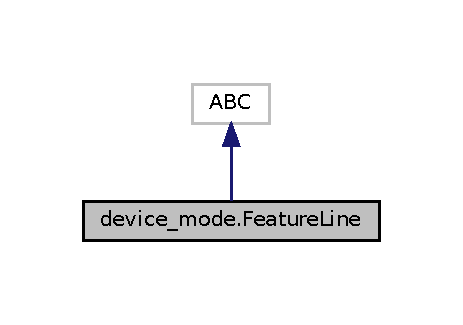
\includegraphics[width=222pt]{classdevice__mode_1_1FeatureLine__inherit__graph}
\end{center}
\end{figure}


Collaboration diagram for device\+\_\+mode.\+Feature\+Line\+:
\nopagebreak
\begin{figure}[H]
\begin{center}
\leavevmode
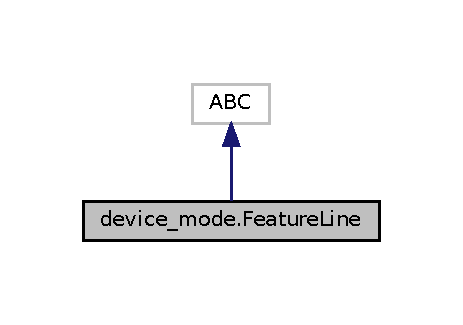
\includegraphics[width=222pt]{classdevice__mode_1_1FeatureLine__coll__graph}
\end{center}
\end{figure}
\subsection*{Public Member Functions}
\begin{DoxyCompactItemize}
\item 
def \hyperlink{classdevice__mode_1_1FeatureLine_a1abbb99081dc21c569cba237c859dae5}{generate\+\_\+data\+\_\+files} (self)
\item 
def \hyperlink{classdevice__mode_1_1FeatureLine_a6223a227b982c9eec4035c5d9f3f7e3c}{generate\+\_\+data\+\_\+fields} (self)
\item 
def \hyperlink{classdevice__mode_1_1FeatureLine_a6f2c5a624f255bd290ff74a9f3a29291}{get\+\_\+parsar} (self)
\item 
def \hyperlink{classdevice__mode_1_1FeatureLine_a828523120c977cfd677a8c5146906400}{get\+\_\+gui} (self)
\item 
def \hyperlink{classdevice__mode_1_1FeatureLine_a05270169f8fe514acc1238d70bde0f12}{get\+\_\+struct\+\_\+size} (self)
\item 
def \hyperlink{classdevice__mode_1_1FeatureLine_a2f9a39132e28fc061bb16c96f7e8177e}{generate\+\_\+struct\+\_\+repr} (self)
\end{DoxyCompactItemize}


\subsection{Detailed Description}
\begin{DoxyVerb}Abstract class that defines the implementation for 
describing a feature line for PC end software. 
\end{DoxyVerb}
 

\subsection{Member Function Documentation}
\mbox{\Hypertarget{classdevice__mode_1_1FeatureLine_a6223a227b982c9eec4035c5d9f3f7e3c}\label{classdevice__mode_1_1FeatureLine_a6223a227b982c9eec4035c5d9f3f7e3c}} 
\index{device\+\_\+mode\+::\+Feature\+Line@{device\+\_\+mode\+::\+Feature\+Line}!generate\+\_\+data\+\_\+fields@{generate\+\_\+data\+\_\+fields}}
\index{generate\+\_\+data\+\_\+fields@{generate\+\_\+data\+\_\+fields}!device\+\_\+mode\+::\+Feature\+Line@{device\+\_\+mode\+::\+Feature\+Line}}
\subsubsection{\texorpdfstring{generate\+\_\+data\+\_\+fields()}{generate\_data\_fields()}}
{\footnotesize\ttfamily def device\+\_\+mode.\+Feature\+Line.\+generate\+\_\+data\+\_\+fields (\begin{DoxyParamCaption}\item[{}]{self }\end{DoxyParamCaption})}

\mbox{\Hypertarget{classdevice__mode_1_1FeatureLine_a1abbb99081dc21c569cba237c859dae5}\label{classdevice__mode_1_1FeatureLine_a1abbb99081dc21c569cba237c859dae5}} 
\index{device\+\_\+mode\+::\+Feature\+Line@{device\+\_\+mode\+::\+Feature\+Line}!generate\+\_\+data\+\_\+files@{generate\+\_\+data\+\_\+files}}
\index{generate\+\_\+data\+\_\+files@{generate\+\_\+data\+\_\+files}!device\+\_\+mode\+::\+Feature\+Line@{device\+\_\+mode\+::\+Feature\+Line}}
\subsubsection{\texorpdfstring{generate\+\_\+data\+\_\+files()}{generate\_data\_files()}}
{\footnotesize\ttfamily def device\+\_\+mode.\+Feature\+Line.\+generate\+\_\+data\+\_\+files (\begin{DoxyParamCaption}\item[{}]{self }\end{DoxyParamCaption})}

\mbox{\Hypertarget{classdevice__mode_1_1FeatureLine_a2f9a39132e28fc061bb16c96f7e8177e}\label{classdevice__mode_1_1FeatureLine_a2f9a39132e28fc061bb16c96f7e8177e}} 
\index{device\+\_\+mode\+::\+Feature\+Line@{device\+\_\+mode\+::\+Feature\+Line}!generate\+\_\+struct\+\_\+repr@{generate\+\_\+struct\+\_\+repr}}
\index{generate\+\_\+struct\+\_\+repr@{generate\+\_\+struct\+\_\+repr}!device\+\_\+mode\+::\+Feature\+Line@{device\+\_\+mode\+::\+Feature\+Line}}
\subsubsection{\texorpdfstring{generate\+\_\+struct\+\_\+repr()}{generate\_struct\_repr()}}
{\footnotesize\ttfamily def device\+\_\+mode.\+Feature\+Line.\+generate\+\_\+struct\+\_\+repr (\begin{DoxyParamCaption}\item[{}]{self }\end{DoxyParamCaption})}

\mbox{\Hypertarget{classdevice__mode_1_1FeatureLine_a828523120c977cfd677a8c5146906400}\label{classdevice__mode_1_1FeatureLine_a828523120c977cfd677a8c5146906400}} 
\index{device\+\_\+mode\+::\+Feature\+Line@{device\+\_\+mode\+::\+Feature\+Line}!get\+\_\+gui@{get\+\_\+gui}}
\index{get\+\_\+gui@{get\+\_\+gui}!device\+\_\+mode\+::\+Feature\+Line@{device\+\_\+mode\+::\+Feature\+Line}}
\subsubsection{\texorpdfstring{get\+\_\+gui()}{get\_gui()}}
{\footnotesize\ttfamily def device\+\_\+mode.\+Feature\+Line.\+get\+\_\+gui (\begin{DoxyParamCaption}\item[{}]{self }\end{DoxyParamCaption})}

\mbox{\Hypertarget{classdevice__mode_1_1FeatureLine_a6f2c5a624f255bd290ff74a9f3a29291}\label{classdevice__mode_1_1FeatureLine_a6f2c5a624f255bd290ff74a9f3a29291}} 
\index{device\+\_\+mode\+::\+Feature\+Line@{device\+\_\+mode\+::\+Feature\+Line}!get\+\_\+parsar@{get\+\_\+parsar}}
\index{get\+\_\+parsar@{get\+\_\+parsar}!device\+\_\+mode\+::\+Feature\+Line@{device\+\_\+mode\+::\+Feature\+Line}}
\subsubsection{\texorpdfstring{get\+\_\+parsar()}{get\_parsar()}}
{\footnotesize\ttfamily def device\+\_\+mode.\+Feature\+Line.\+get\+\_\+parsar (\begin{DoxyParamCaption}\item[{}]{self }\end{DoxyParamCaption})}

\mbox{\Hypertarget{classdevice__mode_1_1FeatureLine_a05270169f8fe514acc1238d70bde0f12}\label{classdevice__mode_1_1FeatureLine_a05270169f8fe514acc1238d70bde0f12}} 
\index{device\+\_\+mode\+::\+Feature\+Line@{device\+\_\+mode\+::\+Feature\+Line}!get\+\_\+struct\+\_\+size@{get\+\_\+struct\+\_\+size}}
\index{get\+\_\+struct\+\_\+size@{get\+\_\+struct\+\_\+size}!device\+\_\+mode\+::\+Feature\+Line@{device\+\_\+mode\+::\+Feature\+Line}}
\subsubsection{\texorpdfstring{get\+\_\+struct\+\_\+size()}{get\_struct\_size()}}
{\footnotesize\ttfamily def device\+\_\+mode.\+Feature\+Line.\+get\+\_\+struct\+\_\+size (\begin{DoxyParamCaption}\item[{}]{self }\end{DoxyParamCaption})}



The documentation for this class was generated from the following file\+:\begin{DoxyCompactItemize}
\item 
code/pc\+\_\+app/\hyperlink{device__mode_8py}{device\+\_\+mode.\+py}\end{DoxyCompactItemize}

\hypertarget{classInterArrivalTime}{}\section{Inter\+Arrival\+Time$<$ Counter\+Type, C\+P\+U\+Tick\+Type $>$ Class Template Reference}
\label{classInterArrivalTime}\index{Inter\+Arrival\+Time$<$ Counter\+Type, C\+P\+U\+Tick\+Type $>$@{Inter\+Arrival\+Time$<$ Counter\+Type, C\+P\+U\+Tick\+Type $>$}}


{\ttfamily \#include $<$interarrival.\+hpp$>$}



Collaboration diagram for Inter\+Arrival\+Time$<$ Counter\+Type, C\+P\+U\+Tick\+Type $>$\+:
\nopagebreak
\begin{figure}[H]
\begin{center}
\leavevmode
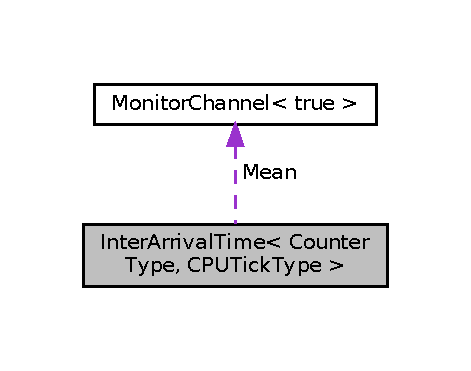
\includegraphics[width=226pt]{classInterArrivalTime__coll__graph}
\end{center}
\end{figure}
\subsection*{Public Member Functions}
\begin{DoxyCompactItemize}
\item 
constexpr \hyperlink{classInterArrivalTime_a2b5ea12da6c38e85b7e92403abcade5f}{Inter\+Arrival\+Time} (const Counter\+Type $\ast$cntr\+\_\+location)
\begin{DoxyCompactList}\small\item\em Constructor that accepts the counter location, that it frequently samples. It only accepts {\ttfamily unsigned int} types. \end{DoxyCompactList}\item 
void \hyperlink{classInterArrivalTime_a2da37f684151d0cfefb97b50fcffd9a0}{measure} () \+\_\+\+\_\+attribute\+\_\+\+\_\+((flatten))
\begin{DoxyCompactList}\small\item\em Measures the difference between two {\itshape observable} counts. If the mean is closer to 1, the pulse inter-\/arrival time will be implemented later using the C\+PU cycle count. \end{DoxyCompactList}\item 
void \hyperlink{classInterArrivalTime_a8a12081f1132d4a2c7a3898b01897c8d}{output} () \+\_\+\+\_\+attribute\+\_\+\+\_\+((always\+\_\+inline))
\begin{DoxyCompactList}\small\item\em Outputs the calculated statistics as a binary struct. \end{DoxyCompactList}\end{DoxyCompactItemize}
\subsection*{Public Attributes}
\begin{DoxyCompactItemize}
\item 
Counter\+Type $\ast$ \hyperlink{classInterArrivalTime_a6873d0052064c8db918fd0a813524c6f}{Cntr}
\begin{DoxyCompactList}\small\item\em Saves the address of the counter location. \end{DoxyCompactList}\item 
Counter\+Type \hyperlink{classInterArrivalTime_ac73e4d6bbfc5daea67b53723ede5e9fd}{Count\+Diff} = 0
\begin{DoxyCompactList}\small\item\em The difference between the arrival time of last two photons. \end{DoxyCompactList}\item 
Counter\+Type \hyperlink{classInterArrivalTime_a8a24e1acb445c45b2934955fb0dcc8f5}{Last\+Cntr} = 0
\begin{DoxyCompactList}\small\item\em Last Counter value recorded. \end{DoxyCompactList}\item 
Counter\+Type \hyperlink{classInterArrivalTime_aa0126b0de317f9b1b7660cfe305b5779}{Now} = 0
\begin{DoxyCompactList}\small\item\em Current Counter value storage. \end{DoxyCompactList}\item 
\hyperlink{classMonitorChannel}{Monitor\+Channel}$<$ true $>$ \hyperlink{classInterArrivalTime_a108e8d20e7a26f7b9b6ac75c38632cd0}{Mean}
\begin{DoxyCompactList}\small\item\em Mean Inter-\/arrival time. \end{DoxyCompactList}\end{DoxyCompactItemize}
\subsection*{Private Member Functions}
\begin{DoxyCompactItemize}
\item 
Counter\+Type \hyperlink{classInterArrivalTime_a64985dc80cad0a2e79718bad59ca7341}{get\+\_\+counter} () \+\_\+\+\_\+attribute\+\_\+\+\_\+((always\+\_\+inline))
\end{DoxyCompactItemize}


\subsection{Constructor \& Destructor Documentation}
\mbox{\Hypertarget{classInterArrivalTime_a2b5ea12da6c38e85b7e92403abcade5f}\label{classInterArrivalTime_a2b5ea12da6c38e85b7e92403abcade5f}} 
\index{Inter\+Arrival\+Time@{Inter\+Arrival\+Time}!Inter\+Arrival\+Time@{Inter\+Arrival\+Time}}
\index{Inter\+Arrival\+Time@{Inter\+Arrival\+Time}!Inter\+Arrival\+Time@{Inter\+Arrival\+Time}}
\subsubsection{\texorpdfstring{Inter\+Arrival\+Time()}{InterArrivalTime()}}
{\footnotesize\ttfamily template$<$typename Counter\+Type , typename C\+P\+U\+Tick\+Type $>$ \\
constexpr \hyperlink{classInterArrivalTime}{Inter\+Arrival\+Time}$<$ Counter\+Type, C\+P\+U\+Tick\+Type $>$\+::\hyperlink{classInterArrivalTime}{Inter\+Arrival\+Time} (\begin{DoxyParamCaption}\item[{const Counter\+Type $\ast$}]{cntr\+\_\+location }\end{DoxyParamCaption})\hspace{0.3cm}{\ttfamily [inline]}}



Constructor that accepts the counter location, that it frequently samples. It only accepts {\ttfamily unsigned int} types. 



\subsection{Member Function Documentation}
\mbox{\Hypertarget{classInterArrivalTime_a64985dc80cad0a2e79718bad59ca7341}\label{classInterArrivalTime_a64985dc80cad0a2e79718bad59ca7341}} 
\index{Inter\+Arrival\+Time@{Inter\+Arrival\+Time}!get\+\_\+counter@{get\+\_\+counter}}
\index{get\+\_\+counter@{get\+\_\+counter}!Inter\+Arrival\+Time@{Inter\+Arrival\+Time}}
\subsubsection{\texorpdfstring{get\+\_\+counter()}{get\_counter()}}
{\footnotesize\ttfamily template$<$typename Counter\+Type , typename C\+P\+U\+Tick\+Type $>$ \\
Counter\+Type \hyperlink{classInterArrivalTime}{Inter\+Arrival\+Time}$<$ Counter\+Type, C\+P\+U\+Tick\+Type $>$\+::get\+\_\+counter (\begin{DoxyParamCaption}{ }\end{DoxyParamCaption})\hspace{0.3cm}{\ttfamily [inline]}, {\ttfamily [private]}}

\mbox{\Hypertarget{classInterArrivalTime_a2da37f684151d0cfefb97b50fcffd9a0}\label{classInterArrivalTime_a2da37f684151d0cfefb97b50fcffd9a0}} 
\index{Inter\+Arrival\+Time@{Inter\+Arrival\+Time}!measure@{measure}}
\index{measure@{measure}!Inter\+Arrival\+Time@{Inter\+Arrival\+Time}}
\subsubsection{\texorpdfstring{measure()}{measure()}}
{\footnotesize\ttfamily template$<$typename Counter\+Type , typename C\+P\+U\+Tick\+Type $>$ \\
void \hyperlink{classInterArrivalTime}{Inter\+Arrival\+Time}$<$ Counter\+Type, C\+P\+U\+Tick\+Type $>$\+::measure (\begin{DoxyParamCaption}{ }\end{DoxyParamCaption})\hspace{0.3cm}{\ttfamily [inline]}}



Measures the difference between two {\itshape observable} counts. If the mean is closer to 1, the pulse inter-\/arrival time will be implemented later using the C\+PU cycle count. 

\mbox{\Hypertarget{classInterArrivalTime_a8a12081f1132d4a2c7a3898b01897c8d}\label{classInterArrivalTime_a8a12081f1132d4a2c7a3898b01897c8d}} 
\index{Inter\+Arrival\+Time@{Inter\+Arrival\+Time}!output@{output}}
\index{output@{output}!Inter\+Arrival\+Time@{Inter\+Arrival\+Time}}
\subsubsection{\texorpdfstring{output()}{output()}}
{\footnotesize\ttfamily template$<$typename Counter\+Type , typename C\+P\+U\+Tick\+Type $>$ \\
void \hyperlink{classInterArrivalTime}{Inter\+Arrival\+Time}$<$ Counter\+Type, C\+P\+U\+Tick\+Type $>$\+::output (\begin{DoxyParamCaption}{ }\end{DoxyParamCaption})\hspace{0.3cm}{\ttfamily [inline]}}



Outputs the calculated statistics as a binary struct. 



\subsection{Member Data Documentation}
\mbox{\Hypertarget{classInterArrivalTime_a6873d0052064c8db918fd0a813524c6f}\label{classInterArrivalTime_a6873d0052064c8db918fd0a813524c6f}} 
\index{Inter\+Arrival\+Time@{Inter\+Arrival\+Time}!Cntr@{Cntr}}
\index{Cntr@{Cntr}!Inter\+Arrival\+Time@{Inter\+Arrival\+Time}}
\subsubsection{\texorpdfstring{Cntr}{Cntr}}
{\footnotesize\ttfamily template$<$typename Counter\+Type , typename C\+P\+U\+Tick\+Type $>$ \\
Counter\+Type$\ast$ \hyperlink{classInterArrivalTime}{Inter\+Arrival\+Time}$<$ Counter\+Type, C\+P\+U\+Tick\+Type $>$\+::Cntr}



Saves the address of the counter location. 

\mbox{\Hypertarget{classInterArrivalTime_ac73e4d6bbfc5daea67b53723ede5e9fd}\label{classInterArrivalTime_ac73e4d6bbfc5daea67b53723ede5e9fd}} 
\index{Inter\+Arrival\+Time@{Inter\+Arrival\+Time}!Count\+Diff@{Count\+Diff}}
\index{Count\+Diff@{Count\+Diff}!Inter\+Arrival\+Time@{Inter\+Arrival\+Time}}
\subsubsection{\texorpdfstring{Count\+Diff}{CountDiff}}
{\footnotesize\ttfamily template$<$typename Counter\+Type , typename C\+P\+U\+Tick\+Type $>$ \\
Counter\+Type \hyperlink{classInterArrivalTime}{Inter\+Arrival\+Time}$<$ Counter\+Type, C\+P\+U\+Tick\+Type $>$\+::Count\+Diff = 0}



The difference between the arrival time of last two photons. 

\mbox{\Hypertarget{classInterArrivalTime_a8a24e1acb445c45b2934955fb0dcc8f5}\label{classInterArrivalTime_a8a24e1acb445c45b2934955fb0dcc8f5}} 
\index{Inter\+Arrival\+Time@{Inter\+Arrival\+Time}!Last\+Cntr@{Last\+Cntr}}
\index{Last\+Cntr@{Last\+Cntr}!Inter\+Arrival\+Time@{Inter\+Arrival\+Time}}
\subsubsection{\texorpdfstring{Last\+Cntr}{LastCntr}}
{\footnotesize\ttfamily template$<$typename Counter\+Type , typename C\+P\+U\+Tick\+Type $>$ \\
Counter\+Type \hyperlink{classInterArrivalTime}{Inter\+Arrival\+Time}$<$ Counter\+Type, C\+P\+U\+Tick\+Type $>$\+::Last\+Cntr = 0}



Last Counter value recorded. 

\mbox{\Hypertarget{classInterArrivalTime_a108e8d20e7a26f7b9b6ac75c38632cd0}\label{classInterArrivalTime_a108e8d20e7a26f7b9b6ac75c38632cd0}} 
\index{Inter\+Arrival\+Time@{Inter\+Arrival\+Time}!Mean@{Mean}}
\index{Mean@{Mean}!Inter\+Arrival\+Time@{Inter\+Arrival\+Time}}
\subsubsection{\texorpdfstring{Mean}{Mean}}
{\footnotesize\ttfamily template$<$typename Counter\+Type , typename C\+P\+U\+Tick\+Type $>$ \\
\hyperlink{classMonitorChannel}{Monitor\+Channel}$<$true$>$ \hyperlink{classInterArrivalTime}{Inter\+Arrival\+Time}$<$ Counter\+Type, C\+P\+U\+Tick\+Type $>$\+::Mean}



Mean Inter-\/arrival time. 

\mbox{\Hypertarget{classInterArrivalTime_aa0126b0de317f9b1b7660cfe305b5779}\label{classInterArrivalTime_aa0126b0de317f9b1b7660cfe305b5779}} 
\index{Inter\+Arrival\+Time@{Inter\+Arrival\+Time}!Now@{Now}}
\index{Now@{Now}!Inter\+Arrival\+Time@{Inter\+Arrival\+Time}}
\subsubsection{\texorpdfstring{Now}{Now}}
{\footnotesize\ttfamily template$<$typename Counter\+Type , typename C\+P\+U\+Tick\+Type $>$ \\
Counter\+Type \hyperlink{classInterArrivalTime}{Inter\+Arrival\+Time}$<$ Counter\+Type, C\+P\+U\+Tick\+Type $>$\+::Now = 0}



Current Counter value storage. 



The documentation for this class was generated from the following file\+:\begin{DoxyCompactItemize}
\item 
code/hardware/\hyperlink{interarrival_8hpp}{interarrival.\+hpp}\end{DoxyCompactItemize}

\hypertarget{classLEDSet}{}\section{L\+E\+D\+Set$<$ S\+E\+T\+\_\+\+S\+I\+ZE $>$ Class Template Reference}
\label{classLEDSet}\index{L\+E\+D\+Set$<$ S\+E\+T\+\_\+\+S\+I\+Z\+E $>$@{L\+E\+D\+Set$<$ S\+E\+T\+\_\+\+S\+I\+Z\+E $>$}}


{\ttfamily \#include $<$ledset.\+hpp$>$}

\subsection*{Public Types}
\begin{DoxyCompactItemize}
\item 
enum \hyperlink{classLEDSet_ae26a13b2d33c51351bc6d0acdf2a94a4}{ledstate\+\_\+t} \{ \hyperlink{classLEDSet_ae26a13b2d33c51351bc6d0acdf2a94a4a786545571f352fd284991e5fcdb79238}{O\+FF} = 0, 
\hyperlink{classLEDSet_ae26a13b2d33c51351bc6d0acdf2a94a4a1e073152d5525648a5bb26cf3eb98ea2}{ON} = 1, 
\hyperlink{classLEDSet_ae26a13b2d33c51351bc6d0acdf2a94a4a2c0806958e37c8d87bd57df8990b30eb}{Analog} = 2
 \}
\end{DoxyCompactItemize}
\subsection*{Public Member Functions}
\begin{DoxyCompactItemize}
\item 
\hyperlink{classLEDSet_a0d3339102ac73fb691f823bcd31a84b9}{L\+E\+D\+Set} (std\+::initializer\+\_\+list$<$ unsigned int $>$ pins)
\begin{DoxyCompactList}\small\item\em Constructor for \hyperlink{classLEDSet}{L\+E\+D\+Set} class. \end{DoxyCompactList}\item 
unsigned int \hyperlink{classLEDSet_a0d153646b1a750421af1f3617d90ad04}{size} () \+\_\+\+\_\+attribute\+\_\+\+\_\+((always\+\_\+inline))
\begin{DoxyCompactList}\small\item\em Returns the size of the led sets. \end{DoxyCompactList}\item 
void \hyperlink{classLEDSet_aae4545d8f8cb6e41a3c2960fb7369e48}{init} ()
\begin{DoxyCompactList}\small\item\em Sets up the pin mode of all L\+E\+Ds. \end{DoxyCompactList}\item 
void \hyperlink{classLEDSet_a520061aaf788486d2aa3aa3dfb3e32d6}{state\+\_\+reload} ()
\begin{DoxyCompactList}\small\item\em Sets the L\+E\+Ds based on the value of the corresponding state variable. This function is useful when the state is altered seperately from the digital\+Write calls. The function also calls pin\+Mode() which muxes the pins to gpio. For State == Analog\+: The state maintains the analog dim state. \end{DoxyCompactList}\item 
void \hyperlink{classLEDSet_a141bb664e7f58ae676455972ca9cd686}{O\+N\+\_\+todigital} ()
\begin{DoxyCompactList}\small\item\em Sets all leds with states (ON == 1) and (Analog == 2) to (ON == 1). \end{DoxyCompactList}\item 
void \hyperlink{classLEDSet_ae2bcd287ff637c2600603e83b0981c77}{toggle\+\_\+all} ()
\begin{DoxyCompactList}\small\item\em Toggles the state of all the L\+E\+Ds. This is a pure digital function and destroys all Analog dim states. \end{DoxyCompactList}\item 
void \hyperlink{classLEDSet_a6062da843aabdf8fbdcedb70fed00dec}{toggle\+\_\+twice} (int pin, double time\+\_\+ms)
\begin{DoxyCompactList}\small\item\em Toggles the state of a particular L\+ED. This is a pure digital function and destroys all Analog dim states. \end{DoxyCompactList}\item 
void \hyperlink{classLEDSet_a61cc024950a5b66dff34c449cc73787f}{toggle\+\_\+all\+\_\+routine} (int delay\+\_\+ms)
\item 
void \hyperlink{classLEDSet_a8a5ef40584236c3793e4274688eac379}{dim} (int pin, unsigned int analog\+\_\+val)
\begin{DoxyCompactList}\small\item\em dims a particular valid led pin. \end{DoxyCompactList}\item 
void \hyperlink{classLEDSet_ad8313aa0c4fc34cd3481db0fade6318c}{dim\+\_\+all} (unsigned int analog\+\_\+val)
\begin{DoxyCompactList}\small\item\em Dims the O\+N-\/\+L\+E\+Ds with the provided analog voltage. Only affects L\+E\+Ds that are ON or on Analog Mode. \end{DoxyCompactList}\item 
void \hyperlink{classLEDSet_a30c6efe7fc286c3d0a7e2ac210dd2c1e}{dim\+\_\+all\+\_\+routine} (unsigned int end\+\_\+analog\+\_\+val, double time\+\_\+s)
\item 
void \hyperlink{classLEDSet_a73dae073882d369a9cc9b9a93f446157}{max\+\_\+bright\+\_\+all} ()
\begin{DoxyCompactList}\small\item\em Sets maximum brightness for all O\+N-\/\+L\+E\+Ds. \end{DoxyCompactList}\item 
void \hyperlink{classLEDSet_a9479e36e91b5b1387cfc27722a4a6007}{min\+\_\+bright\+\_\+all} ()
\item 
void \hyperlink{classLEDSet_aaebfea59ba933621c4f7d7d405119702}{set\+\_\+all} () \+\_\+\+\_\+attribute\+\_\+\+\_\+((always\+\_\+inline))
\begin{DoxyCompactList}\small\item\em Turn on all available L\+E\+Ds. \end{DoxyCompactList}\item 
void \hyperlink{classLEDSet_aabff2609d8df733936dda53d60302b72}{unset\+\_\+all} () \+\_\+\+\_\+attribute\+\_\+\+\_\+((always\+\_\+inline))
\item 
void \hyperlink{classLEDSet_a8f5431c0b3c059c43353cf7e3d02ca62}{set} (int led\+\_\+pin) \+\_\+\+\_\+attribute\+\_\+\+\_\+((always\+\_\+inline))
\begin{DoxyCompactList}\small\item\em Turn-\/\+ON a particular L\+ED Pin. \end{DoxyCompactList}\item 
void \hyperlink{classLEDSet_aacc3566d74c4051350977b578ada3a4d}{unset} (int led\+\_\+pin) \+\_\+\+\_\+attribute\+\_\+\+\_\+((always\+\_\+inline))
\begin{DoxyCompactList}\small\item\em Turn-\/\+O\+FF a particular L\+ED Pin. \end{DoxyCompactList}\item 
void \hyperlink{classLEDSet_a9912385e65dddd78cf0f41cce4fbcba2}{set} (int led\+\_\+pin1, int led\+\_\+pin2) \+\_\+\+\_\+attribute\+\_\+\+\_\+((always\+\_\+inline))
\begin{DoxyCompactList}\small\item\em Turn-\/\+ON two L\+ED Pins simultaneously. The function only works if both the Pins are valid pins. \end{DoxyCompactList}\item 
void \hyperlink{classLEDSet_ac84aa5b9e72689bbfd71f556995dfe03}{unset} (int led\+\_\+pin1, int led\+\_\+pin2) \+\_\+\+\_\+attribute\+\_\+\+\_\+((always\+\_\+inline))
\begin{DoxyCompactList}\small\item\em Turn-\/\+O\+FF two L\+ED Pins simultaneously. \end{DoxyCompactList}\item 
void \hyperlink{classLEDSet_a5dba15c24ec18e11f82368d203ceb9f1}{set} (int led\+\_\+pin1, int led\+\_\+pin2, int led\+\_\+pin3) \+\_\+\+\_\+attribute\+\_\+\+\_\+((always\+\_\+inline))
\begin{DoxyCompactList}\small\item\em Turn-\/\+ON three L\+ED Pins simultaneously. \end{DoxyCompactList}\item 
void \hyperlink{classLEDSet_a1a6a52e4fd96dd8500861df0a9d0066d}{unset} (int led\+\_\+pin1, int led\+\_\+pin2, int led\+\_\+pin3) \+\_\+\+\_\+attribute\+\_\+\+\_\+((always\+\_\+inline))
\begin{DoxyCompactList}\small\item\em Turn-\/\+FF three L\+ED Pins simultaneously. \end{DoxyCompactList}\item 
void \hyperlink{classLEDSet_aa392b74b090de60a25f7577195327afd}{error} (int pin)
\begin{DoxyCompactList}\small\item\em Special function that sets a valid pin and sets the flag {\ttfamily Led\+Set\+::\+Error\+\_\+\+State} to true. This function also clears all L\+ED states prior to the Error State but does not modify states set after the error state. \end{DoxyCompactList}\item 
void \hyperlink{classLEDSet_aafb42531245febe55685c764c29d918f}{assert\+\_\+errors} ()
\begin{DoxyCompactList}\small\item\em Special function that initiates a special routine if the device is in the Error State. It also calls {\ttfamily abort()} , if that feature macro is enabled. \end{DoxyCompactList}\item 
bool \hyperlink{classLEDSet_ab3c7ec4740bab77f762dcd48fba26579}{is\+\_\+valid\+\_\+pin} (int pin)
\begin{DoxyCompactList}\small\item\em Returns whether the given pin is a \char`\"{}valid pin\char`\"{}. A valid pin is a pin that is registered with the \hyperlink{classLEDSet}{L\+E\+D\+Set}. \end{DoxyCompactList}\end{DoxyCompactItemize}
\subsection*{Public Attributes}
\begin{DoxyCompactItemize}
\item 
const int \hyperlink{classLEDSet_a76dfe34c89f6161184583a5ffdcad2e1}{L\+E\+Ds} \mbox{[}S\+E\+T\+\_\+\+S\+I\+ZE\mbox{]} = \{\hyperlink{pins_8hpp_a2b2fb4f846b45d396215a25f949a1bc7}{S\+A\+F\+E\+\_\+\+O\+U\+T\+P\+U\+T\+\_\+\+D\+U\+M\+P\+\_\+\+P\+IN}\}
\begin{DoxyCompactList}\small\item\em L\+ED pins. \end{DoxyCompactList}\item 
unsigned int \hyperlink{classLEDSet_a7185bf98d8866da93847fde7b2145cc4}{State} \mbox{[}S\+E\+T\+\_\+\+S\+I\+ZE\mbox{]}
\begin{DoxyCompactList}\small\item\em O\+N-\/\+O\+F\+F/\+Analog states for all L\+E\+Ds. \end{DoxyCompactList}\item 
bool \hyperlink{classLEDSet_af9c6ea1d0006d7427c82e8e56f9f2de5}{Error\+\_\+\+State} = false
\begin{DoxyCompactList}\small\item\em Whether the L\+ED Panel is in an error state. \end{DoxyCompactList}\end{DoxyCompactItemize}
\subsection*{Private Member Functions}
\begin{DoxyCompactItemize}
\item 
int \hyperlink{classLEDSet_a4ffb3b4a8a5cffdc03f4040ff67a33e9}{fetch\+\_\+index} (int pin) \+\_\+\+\_\+attribute\+\_\+\+\_\+((always\+\_\+inline))
\begin{DoxyCompactList}\small\item\em Retrive data structure index based on the pin number. Returns -\/1 if the pin was not found. \end{DoxyCompactList}\end{DoxyCompactItemize}


\subsection{Detailed Description}
\subsubsection*{template$<$unsigned int S\+E\+T\+\_\+\+S\+I\+ZE$>$\newline
class L\+E\+D\+Set$<$ S\+E\+T\+\_\+\+S\+I\+Z\+E $>$}

an interface for accessing the L\+E\+Ds on the dashboar. The object serves primarily as a bookeeping object, and hence, enables state conservation and switching, and automatically manages dimming, and complex routines. 

\subsection{Member Enumeration Documentation}
\mbox{\Hypertarget{classLEDSet_ae26a13b2d33c51351bc6d0acdf2a94a4}\label{classLEDSet_ae26a13b2d33c51351bc6d0acdf2a94a4}} 
\index{L\+E\+D\+Set@{L\+E\+D\+Set}!ledstate\+\_\+t@{ledstate\+\_\+t}}
\index{ledstate\+\_\+t@{ledstate\+\_\+t}!L\+E\+D\+Set@{L\+E\+D\+Set}}
\subsubsection{\texorpdfstring{ledstate\+\_\+t}{ledstate\_t}}
{\footnotesize\ttfamily template$<$unsigned int S\+E\+T\+\_\+\+S\+I\+ZE$>$ \\
enum \hyperlink{classLEDSet_ae26a13b2d33c51351bc6d0acdf2a94a4}{L\+E\+D\+Set\+::ledstate\+\_\+t}}

\begin{DoxyEnumFields}{Enumerator}
\raisebox{\heightof{T}}[0pt][0pt]{\index{O\+FF@{O\+FF}!L\+E\+D\+Set@{L\+E\+D\+Set}}\index{L\+E\+D\+Set@{L\+E\+D\+Set}!O\+FF@{O\+FF}}}\mbox{\Hypertarget{classLEDSet_ae26a13b2d33c51351bc6d0acdf2a94a4a786545571f352fd284991e5fcdb79238}\label{classLEDSet_ae26a13b2d33c51351bc6d0acdf2a94a4a786545571f352fd284991e5fcdb79238}} 
O\+FF&\\
\hline

\raisebox{\heightof{T}}[0pt][0pt]{\index{ON@{ON}!L\+E\+D\+Set@{L\+E\+D\+Set}}\index{L\+E\+D\+Set@{L\+E\+D\+Set}!ON@{ON}}}\mbox{\Hypertarget{classLEDSet_ae26a13b2d33c51351bc6d0acdf2a94a4a1e073152d5525648a5bb26cf3eb98ea2}\label{classLEDSet_ae26a13b2d33c51351bc6d0acdf2a94a4a1e073152d5525648a5bb26cf3eb98ea2}} 
ON&\\
\hline

\raisebox{\heightof{T}}[0pt][0pt]{\index{Analog@{Analog}!L\+E\+D\+Set@{L\+E\+D\+Set}}\index{L\+E\+D\+Set@{L\+E\+D\+Set}!Analog@{Analog}}}\mbox{\Hypertarget{classLEDSet_ae26a13b2d33c51351bc6d0acdf2a94a4a2c0806958e37c8d87bd57df8990b30eb}\label{classLEDSet_ae26a13b2d33c51351bc6d0acdf2a94a4a2c0806958e37c8d87bd57df8990b30eb}} 
Analog&\\
\hline

\end{DoxyEnumFields}


\subsection{Constructor \& Destructor Documentation}
\mbox{\Hypertarget{classLEDSet_a0d3339102ac73fb691f823bcd31a84b9}\label{classLEDSet_a0d3339102ac73fb691f823bcd31a84b9}} 
\index{L\+E\+D\+Set@{L\+E\+D\+Set}!L\+E\+D\+Set@{L\+E\+D\+Set}}
\index{L\+E\+D\+Set@{L\+E\+D\+Set}!L\+E\+D\+Set@{L\+E\+D\+Set}}
\subsubsection{\texorpdfstring{L\+E\+D\+Set()}{LEDSet()}}
{\footnotesize\ttfamily template$<$unsigned int S\+E\+T\+\_\+\+S\+I\+ZE$>$ \\
\hyperlink{classLEDSet}{L\+E\+D\+Set}$<$ S\+E\+T\+\_\+\+S\+I\+ZE $>$\+::\hyperlink{classLEDSet}{L\+E\+D\+Set} (\begin{DoxyParamCaption}\item[{std\+::initializer\+\_\+list$<$ unsigned int $>$}]{pins }\end{DoxyParamCaption})\hspace{0.3cm}{\ttfamily [inline]}}



Constructor for \hyperlink{classLEDSet}{L\+E\+D\+Set} class. 


\begin{DoxyParams}{Parameters}
{\em pins} & -\/ list of L\+ED pins. \\
\hline
\end{DoxyParams}


\subsection{Member Function Documentation}
\mbox{\Hypertarget{classLEDSet_aafb42531245febe55685c764c29d918f}\label{classLEDSet_aafb42531245febe55685c764c29d918f}} 
\index{L\+E\+D\+Set@{L\+E\+D\+Set}!assert\+\_\+errors@{assert\+\_\+errors}}
\index{assert\+\_\+errors@{assert\+\_\+errors}!L\+E\+D\+Set@{L\+E\+D\+Set}}
\subsubsection{\texorpdfstring{assert\+\_\+errors()}{assert\_errors()}}
{\footnotesize\ttfamily template$<$unsigned int S\+E\+T\+\_\+\+S\+I\+ZE$>$ \\
void \hyperlink{classLEDSet}{L\+E\+D\+Set}$<$ S\+E\+T\+\_\+\+S\+I\+ZE $>$\+::assert\+\_\+errors (\begin{DoxyParamCaption}{ }\end{DoxyParamCaption})\hspace{0.3cm}{\ttfamily [inline]}}



Special function that initiates a special routine if the device is in the Error State. It also calls {\ttfamily abort()} , if that feature macro is enabled. 

\mbox{\Hypertarget{classLEDSet_a8a5ef40584236c3793e4274688eac379}\label{classLEDSet_a8a5ef40584236c3793e4274688eac379}} 
\index{L\+E\+D\+Set@{L\+E\+D\+Set}!dim@{dim}}
\index{dim@{dim}!L\+E\+D\+Set@{L\+E\+D\+Set}}
\subsubsection{\texorpdfstring{dim()}{dim()}}
{\footnotesize\ttfamily template$<$unsigned int S\+E\+T\+\_\+\+S\+I\+ZE$>$ \\
void \hyperlink{classLEDSet}{L\+E\+D\+Set}$<$ S\+E\+T\+\_\+\+S\+I\+ZE $>$\+::dim (\begin{DoxyParamCaption}\item[{int}]{pin,  }\item[{unsigned int}]{analog\+\_\+val }\end{DoxyParamCaption})\hspace{0.3cm}{\ttfamily [inline]}}



dims a particular valid led pin. 

\mbox{\Hypertarget{classLEDSet_ad8313aa0c4fc34cd3481db0fade6318c}\label{classLEDSet_ad8313aa0c4fc34cd3481db0fade6318c}} 
\index{L\+E\+D\+Set@{L\+E\+D\+Set}!dim\+\_\+all@{dim\+\_\+all}}
\index{dim\+\_\+all@{dim\+\_\+all}!L\+E\+D\+Set@{L\+E\+D\+Set}}
\subsubsection{\texorpdfstring{dim\+\_\+all()}{dim\_all()}}
{\footnotesize\ttfamily template$<$unsigned int S\+E\+T\+\_\+\+S\+I\+ZE$>$ \\
void \hyperlink{classLEDSet}{L\+E\+D\+Set}$<$ S\+E\+T\+\_\+\+S\+I\+ZE $>$\+::dim\+\_\+all (\begin{DoxyParamCaption}\item[{unsigned int}]{analog\+\_\+val }\end{DoxyParamCaption})\hspace{0.3cm}{\ttfamily [inline]}}



Dims the O\+N-\/\+L\+E\+Ds with the provided analog voltage. Only affects L\+E\+Ds that are ON or on Analog Mode. 

\mbox{\Hypertarget{classLEDSet_a30c6efe7fc286c3d0a7e2ac210dd2c1e}\label{classLEDSet_a30c6efe7fc286c3d0a7e2ac210dd2c1e}} 
\index{L\+E\+D\+Set@{L\+E\+D\+Set}!dim\+\_\+all\+\_\+routine@{dim\+\_\+all\+\_\+routine}}
\index{dim\+\_\+all\+\_\+routine@{dim\+\_\+all\+\_\+routine}!L\+E\+D\+Set@{L\+E\+D\+Set}}
\subsubsection{\texorpdfstring{dim\+\_\+all\+\_\+routine()}{dim\_all\_routine()}}
{\footnotesize\ttfamily template$<$unsigned int S\+E\+T\+\_\+\+S\+I\+ZE$>$ \\
void \hyperlink{classLEDSet}{L\+E\+D\+Set}$<$ S\+E\+T\+\_\+\+S\+I\+ZE $>$\+::dim\+\_\+all\+\_\+routine (\begin{DoxyParamCaption}\item[{unsigned int}]{end\+\_\+analog\+\_\+val,  }\item[{double}]{time\+\_\+s }\end{DoxyParamCaption})\hspace{0.3cm}{\ttfamily [inline]}}

\mbox{\Hypertarget{classLEDSet_aa392b74b090de60a25f7577195327afd}\label{classLEDSet_aa392b74b090de60a25f7577195327afd}} 
\index{L\+E\+D\+Set@{L\+E\+D\+Set}!error@{error}}
\index{error@{error}!L\+E\+D\+Set@{L\+E\+D\+Set}}
\subsubsection{\texorpdfstring{error()}{error()}}
{\footnotesize\ttfamily template$<$unsigned int S\+E\+T\+\_\+\+S\+I\+ZE$>$ \\
void \hyperlink{classLEDSet}{L\+E\+D\+Set}$<$ S\+E\+T\+\_\+\+S\+I\+ZE $>$\+::error (\begin{DoxyParamCaption}\item[{int}]{pin }\end{DoxyParamCaption})\hspace{0.3cm}{\ttfamily [inline]}}



Special function that sets a valid pin and sets the flag {\ttfamily Led\+Set\+::\+Error\+\_\+\+State} to true. This function also clears all L\+ED states prior to the Error State but does not modify states set after the error state. 

\mbox{\Hypertarget{classLEDSet_a4ffb3b4a8a5cffdc03f4040ff67a33e9}\label{classLEDSet_a4ffb3b4a8a5cffdc03f4040ff67a33e9}} 
\index{L\+E\+D\+Set@{L\+E\+D\+Set}!fetch\+\_\+index@{fetch\+\_\+index}}
\index{fetch\+\_\+index@{fetch\+\_\+index}!L\+E\+D\+Set@{L\+E\+D\+Set}}
\subsubsection{\texorpdfstring{fetch\+\_\+index()}{fetch\_index()}}
{\footnotesize\ttfamily template$<$unsigned int S\+E\+T\+\_\+\+S\+I\+ZE$>$ \\
int \hyperlink{classLEDSet}{L\+E\+D\+Set}$<$ S\+E\+T\+\_\+\+S\+I\+ZE $>$\+::fetch\+\_\+index (\begin{DoxyParamCaption}\item[{int}]{pin }\end{DoxyParamCaption})\hspace{0.3cm}{\ttfamily [inline]}, {\ttfamily [private]}}



Retrive data structure index based on the pin number. Returns -\/1 if the pin was not found. 

\begin{DoxyReturn}{Returns}
Local array index of pin in the L\+E\+Ds array (bookeeping object). -\/1 if the search fails. 
\end{DoxyReturn}
\mbox{\Hypertarget{classLEDSet_aae4545d8f8cb6e41a3c2960fb7369e48}\label{classLEDSet_aae4545d8f8cb6e41a3c2960fb7369e48}} 
\index{L\+E\+D\+Set@{L\+E\+D\+Set}!init@{init}}
\index{init@{init}!L\+E\+D\+Set@{L\+E\+D\+Set}}
\subsubsection{\texorpdfstring{init()}{init()}}
{\footnotesize\ttfamily template$<$unsigned int S\+E\+T\+\_\+\+S\+I\+ZE$>$ \\
void \hyperlink{classLEDSet}{L\+E\+D\+Set}$<$ S\+E\+T\+\_\+\+S\+I\+ZE $>$\+::init (\begin{DoxyParamCaption}{ }\end{DoxyParamCaption})\hspace{0.3cm}{\ttfamily [inline]}}



Sets up the pin mode of all L\+E\+Ds. 

\mbox{\Hypertarget{classLEDSet_ab3c7ec4740bab77f762dcd48fba26579}\label{classLEDSet_ab3c7ec4740bab77f762dcd48fba26579}} 
\index{L\+E\+D\+Set@{L\+E\+D\+Set}!is\+\_\+valid\+\_\+pin@{is\+\_\+valid\+\_\+pin}}
\index{is\+\_\+valid\+\_\+pin@{is\+\_\+valid\+\_\+pin}!L\+E\+D\+Set@{L\+E\+D\+Set}}
\subsubsection{\texorpdfstring{is\+\_\+valid\+\_\+pin()}{is\_valid\_pin()}}
{\footnotesize\ttfamily template$<$unsigned int S\+E\+T\+\_\+\+S\+I\+ZE$>$ \\
bool \hyperlink{classLEDSet}{L\+E\+D\+Set}$<$ S\+E\+T\+\_\+\+S\+I\+ZE $>$\+::is\+\_\+valid\+\_\+pin (\begin{DoxyParamCaption}\item[{int}]{pin }\end{DoxyParamCaption})\hspace{0.3cm}{\ttfamily [inline]}}



Returns whether the given pin is a \char`\"{}valid pin\char`\"{}. A valid pin is a pin that is registered with the \hyperlink{classLEDSet}{L\+E\+D\+Set}. 

\mbox{\Hypertarget{classLEDSet_a73dae073882d369a9cc9b9a93f446157}\label{classLEDSet_a73dae073882d369a9cc9b9a93f446157}} 
\index{L\+E\+D\+Set@{L\+E\+D\+Set}!max\+\_\+bright\+\_\+all@{max\+\_\+bright\+\_\+all}}
\index{max\+\_\+bright\+\_\+all@{max\+\_\+bright\+\_\+all}!L\+E\+D\+Set@{L\+E\+D\+Set}}
\subsubsection{\texorpdfstring{max\+\_\+bright\+\_\+all()}{max\_bright\_all()}}
{\footnotesize\ttfamily template$<$unsigned int S\+E\+T\+\_\+\+S\+I\+ZE$>$ \\
void \hyperlink{classLEDSet}{L\+E\+D\+Set}$<$ S\+E\+T\+\_\+\+S\+I\+ZE $>$\+::max\+\_\+bright\+\_\+all (\begin{DoxyParamCaption}{ }\end{DoxyParamCaption})\hspace{0.3cm}{\ttfamily [inline]}}



Sets maximum brightness for all O\+N-\/\+L\+E\+Ds. 

\mbox{\Hypertarget{classLEDSet_a9479e36e91b5b1387cfc27722a4a6007}\label{classLEDSet_a9479e36e91b5b1387cfc27722a4a6007}} 
\index{L\+E\+D\+Set@{L\+E\+D\+Set}!min\+\_\+bright\+\_\+all@{min\+\_\+bright\+\_\+all}}
\index{min\+\_\+bright\+\_\+all@{min\+\_\+bright\+\_\+all}!L\+E\+D\+Set@{L\+E\+D\+Set}}
\subsubsection{\texorpdfstring{min\+\_\+bright\+\_\+all()}{min\_bright\_all()}}
{\footnotesize\ttfamily template$<$unsigned int S\+E\+T\+\_\+\+S\+I\+ZE$>$ \\
void \hyperlink{classLEDSet}{L\+E\+D\+Set}$<$ S\+E\+T\+\_\+\+S\+I\+ZE $>$\+::min\+\_\+bright\+\_\+all (\begin{DoxyParamCaption}{ }\end{DoxyParamCaption})\hspace{0.3cm}{\ttfamily [inline]}}

Sets the minimum brighness for all O\+N-\/\+L\+E\+Ds. \mbox{\Hypertarget{classLEDSet_a141bb664e7f58ae676455972ca9cd686}\label{classLEDSet_a141bb664e7f58ae676455972ca9cd686}} 
\index{L\+E\+D\+Set@{L\+E\+D\+Set}!O\+N\+\_\+todigital@{O\+N\+\_\+todigital}}
\index{O\+N\+\_\+todigital@{O\+N\+\_\+todigital}!L\+E\+D\+Set@{L\+E\+D\+Set}}
\subsubsection{\texorpdfstring{O\+N\+\_\+todigital()}{ON\_todigital()}}
{\footnotesize\ttfamily template$<$unsigned int S\+E\+T\+\_\+\+S\+I\+ZE$>$ \\
void \hyperlink{classLEDSet}{L\+E\+D\+Set}$<$ S\+E\+T\+\_\+\+S\+I\+ZE $>$\+::O\+N\+\_\+todigital (\begin{DoxyParamCaption}{ }\end{DoxyParamCaption})\hspace{0.3cm}{\ttfamily [inline]}}



Sets all leds with states (ON == 1) and (Analog == 2) to (ON == 1). 

\mbox{\Hypertarget{classLEDSet_a8f5431c0b3c059c43353cf7e3d02ca62}\label{classLEDSet_a8f5431c0b3c059c43353cf7e3d02ca62}} 
\index{L\+E\+D\+Set@{L\+E\+D\+Set}!set@{set}}
\index{set@{set}!L\+E\+D\+Set@{L\+E\+D\+Set}}
\subsubsection{\texorpdfstring{set()}{set()}\hspace{0.1cm}{\footnotesize\ttfamily [1/3]}}
{\footnotesize\ttfamily template$<$unsigned int S\+E\+T\+\_\+\+S\+I\+ZE$>$ \\
void \hyperlink{classLEDSet}{L\+E\+D\+Set}$<$ S\+E\+T\+\_\+\+S\+I\+ZE $>$\+::set (\begin{DoxyParamCaption}\item[{int}]{led\+\_\+pin }\end{DoxyParamCaption})\hspace{0.3cm}{\ttfamily [inline]}}



Turn-\/\+ON a particular L\+ED Pin. 

\mbox{\Hypertarget{classLEDSet_a9912385e65dddd78cf0f41cce4fbcba2}\label{classLEDSet_a9912385e65dddd78cf0f41cce4fbcba2}} 
\index{L\+E\+D\+Set@{L\+E\+D\+Set}!set@{set}}
\index{set@{set}!L\+E\+D\+Set@{L\+E\+D\+Set}}
\subsubsection{\texorpdfstring{set()}{set()}\hspace{0.1cm}{\footnotesize\ttfamily [2/3]}}
{\footnotesize\ttfamily template$<$unsigned int S\+E\+T\+\_\+\+S\+I\+ZE$>$ \\
void \hyperlink{classLEDSet}{L\+E\+D\+Set}$<$ S\+E\+T\+\_\+\+S\+I\+ZE $>$\+::set (\begin{DoxyParamCaption}\item[{int}]{led\+\_\+pin1,  }\item[{int}]{led\+\_\+pin2 }\end{DoxyParamCaption})\hspace{0.3cm}{\ttfamily [inline]}}



Turn-\/\+ON two L\+ED Pins simultaneously. The function only works if both the Pins are valid pins. 

\mbox{\Hypertarget{classLEDSet_a5dba15c24ec18e11f82368d203ceb9f1}\label{classLEDSet_a5dba15c24ec18e11f82368d203ceb9f1}} 
\index{L\+E\+D\+Set@{L\+E\+D\+Set}!set@{set}}
\index{set@{set}!L\+E\+D\+Set@{L\+E\+D\+Set}}
\subsubsection{\texorpdfstring{set()}{set()}\hspace{0.1cm}{\footnotesize\ttfamily [3/3]}}
{\footnotesize\ttfamily template$<$unsigned int S\+E\+T\+\_\+\+S\+I\+ZE$>$ \\
void \hyperlink{classLEDSet}{L\+E\+D\+Set}$<$ S\+E\+T\+\_\+\+S\+I\+ZE $>$\+::set (\begin{DoxyParamCaption}\item[{int}]{led\+\_\+pin1,  }\item[{int}]{led\+\_\+pin2,  }\item[{int}]{led\+\_\+pin3 }\end{DoxyParamCaption})\hspace{0.3cm}{\ttfamily [inline]}}



Turn-\/\+ON three L\+ED Pins simultaneously. 

\mbox{\Hypertarget{classLEDSet_aaebfea59ba933621c4f7d7d405119702}\label{classLEDSet_aaebfea59ba933621c4f7d7d405119702}} 
\index{L\+E\+D\+Set@{L\+E\+D\+Set}!set\+\_\+all@{set\+\_\+all}}
\index{set\+\_\+all@{set\+\_\+all}!L\+E\+D\+Set@{L\+E\+D\+Set}}
\subsubsection{\texorpdfstring{set\+\_\+all()}{set\_all()}}
{\footnotesize\ttfamily template$<$unsigned int S\+E\+T\+\_\+\+S\+I\+ZE$>$ \\
void \hyperlink{classLEDSet}{L\+E\+D\+Set}$<$ S\+E\+T\+\_\+\+S\+I\+ZE $>$\+::set\+\_\+all (\begin{DoxyParamCaption}{ }\end{DoxyParamCaption})\hspace{0.3cm}{\ttfamily [inline]}}



Turn on all available L\+E\+Ds. 

\mbox{\Hypertarget{classLEDSet_a0d153646b1a750421af1f3617d90ad04}\label{classLEDSet_a0d153646b1a750421af1f3617d90ad04}} 
\index{L\+E\+D\+Set@{L\+E\+D\+Set}!size@{size}}
\index{size@{size}!L\+E\+D\+Set@{L\+E\+D\+Set}}
\subsubsection{\texorpdfstring{size()}{size()}}
{\footnotesize\ttfamily template$<$unsigned int S\+E\+T\+\_\+\+S\+I\+ZE$>$ \\
unsigned int \hyperlink{classLEDSet}{L\+E\+D\+Set}$<$ S\+E\+T\+\_\+\+S\+I\+ZE $>$\+::size (\begin{DoxyParamCaption}{ }\end{DoxyParamCaption})\hspace{0.3cm}{\ttfamily [inline]}}



Returns the size of the led sets. 

\mbox{\Hypertarget{classLEDSet_a520061aaf788486d2aa3aa3dfb3e32d6}\label{classLEDSet_a520061aaf788486d2aa3aa3dfb3e32d6}} 
\index{L\+E\+D\+Set@{L\+E\+D\+Set}!state\+\_\+reload@{state\+\_\+reload}}
\index{state\+\_\+reload@{state\+\_\+reload}!L\+E\+D\+Set@{L\+E\+D\+Set}}
\subsubsection{\texorpdfstring{state\+\_\+reload()}{state\_reload()}}
{\footnotesize\ttfamily template$<$unsigned int S\+E\+T\+\_\+\+S\+I\+ZE$>$ \\
void \hyperlink{classLEDSet}{L\+E\+D\+Set}$<$ S\+E\+T\+\_\+\+S\+I\+ZE $>$\+::state\+\_\+reload (\begin{DoxyParamCaption}{ }\end{DoxyParamCaption})\hspace{0.3cm}{\ttfamily [inline]}}



Sets the L\+E\+Ds based on the value of the corresponding state variable. This function is useful when the state is altered seperately from the digital\+Write calls. The function also calls pin\+Mode() which muxes the pins to gpio. For State == Analog\+: The state maintains the analog dim state. 

\mbox{\Hypertarget{classLEDSet_ae2bcd287ff637c2600603e83b0981c77}\label{classLEDSet_ae2bcd287ff637c2600603e83b0981c77}} 
\index{L\+E\+D\+Set@{L\+E\+D\+Set}!toggle\+\_\+all@{toggle\+\_\+all}}
\index{toggle\+\_\+all@{toggle\+\_\+all}!L\+E\+D\+Set@{L\+E\+D\+Set}}
\subsubsection{\texorpdfstring{toggle\+\_\+all()}{toggle\_all()}}
{\footnotesize\ttfamily template$<$unsigned int S\+E\+T\+\_\+\+S\+I\+ZE$>$ \\
void \hyperlink{classLEDSet}{L\+E\+D\+Set}$<$ S\+E\+T\+\_\+\+S\+I\+ZE $>$\+::toggle\+\_\+all (\begin{DoxyParamCaption}{ }\end{DoxyParamCaption})\hspace{0.3cm}{\ttfamily [inline]}}



Toggles the state of all the L\+E\+Ds. This is a pure digital function and destroys all Analog dim states. 

\mbox{\Hypertarget{classLEDSet_a61cc024950a5b66dff34c449cc73787f}\label{classLEDSet_a61cc024950a5b66dff34c449cc73787f}} 
\index{L\+E\+D\+Set@{L\+E\+D\+Set}!toggle\+\_\+all\+\_\+routine@{toggle\+\_\+all\+\_\+routine}}
\index{toggle\+\_\+all\+\_\+routine@{toggle\+\_\+all\+\_\+routine}!L\+E\+D\+Set@{L\+E\+D\+Set}}
\subsubsection{\texorpdfstring{toggle\+\_\+all\+\_\+routine()}{toggle\_all\_routine()}}
{\footnotesize\ttfamily template$<$unsigned int S\+E\+T\+\_\+\+S\+I\+ZE$>$ \\
void \hyperlink{classLEDSet}{L\+E\+D\+Set}$<$ S\+E\+T\+\_\+\+S\+I\+ZE $>$\+::toggle\+\_\+all\+\_\+routine (\begin{DoxyParamCaption}\item[{int}]{delay\+\_\+ms }\end{DoxyParamCaption})\hspace{0.3cm}{\ttfamily [inline]}}

\mbox{\Hypertarget{classLEDSet_a6062da843aabdf8fbdcedb70fed00dec}\label{classLEDSet_a6062da843aabdf8fbdcedb70fed00dec}} 
\index{L\+E\+D\+Set@{L\+E\+D\+Set}!toggle\+\_\+twice@{toggle\+\_\+twice}}
\index{toggle\+\_\+twice@{toggle\+\_\+twice}!L\+E\+D\+Set@{L\+E\+D\+Set}}
\subsubsection{\texorpdfstring{toggle\+\_\+twice()}{toggle\_twice()}}
{\footnotesize\ttfamily template$<$unsigned int S\+E\+T\+\_\+\+S\+I\+ZE$>$ \\
void \hyperlink{classLEDSet}{L\+E\+D\+Set}$<$ S\+E\+T\+\_\+\+S\+I\+ZE $>$\+::toggle\+\_\+twice (\begin{DoxyParamCaption}\item[{int}]{pin,  }\item[{double}]{time\+\_\+ms }\end{DoxyParamCaption})\hspace{0.3cm}{\ttfamily [inline]}}



Toggles the state of a particular L\+ED. This is a pure digital function and destroys all Analog dim states. 

\mbox{\Hypertarget{classLEDSet_aacc3566d74c4051350977b578ada3a4d}\label{classLEDSet_aacc3566d74c4051350977b578ada3a4d}} 
\index{L\+E\+D\+Set@{L\+E\+D\+Set}!unset@{unset}}
\index{unset@{unset}!L\+E\+D\+Set@{L\+E\+D\+Set}}
\subsubsection{\texorpdfstring{unset()}{unset()}\hspace{0.1cm}{\footnotesize\ttfamily [1/3]}}
{\footnotesize\ttfamily template$<$unsigned int S\+E\+T\+\_\+\+S\+I\+ZE$>$ \\
void \hyperlink{classLEDSet}{L\+E\+D\+Set}$<$ S\+E\+T\+\_\+\+S\+I\+ZE $>$\+::unset (\begin{DoxyParamCaption}\item[{int}]{led\+\_\+pin }\end{DoxyParamCaption})\hspace{0.3cm}{\ttfamily [inline]}}



Turn-\/\+O\+FF a particular L\+ED Pin. 

\mbox{\Hypertarget{classLEDSet_ac84aa5b9e72689bbfd71f556995dfe03}\label{classLEDSet_ac84aa5b9e72689bbfd71f556995dfe03}} 
\index{L\+E\+D\+Set@{L\+E\+D\+Set}!unset@{unset}}
\index{unset@{unset}!L\+E\+D\+Set@{L\+E\+D\+Set}}
\subsubsection{\texorpdfstring{unset()}{unset()}\hspace{0.1cm}{\footnotesize\ttfamily [2/3]}}
{\footnotesize\ttfamily template$<$unsigned int S\+E\+T\+\_\+\+S\+I\+ZE$>$ \\
void \hyperlink{classLEDSet}{L\+E\+D\+Set}$<$ S\+E\+T\+\_\+\+S\+I\+ZE $>$\+::unset (\begin{DoxyParamCaption}\item[{int}]{led\+\_\+pin1,  }\item[{int}]{led\+\_\+pin2 }\end{DoxyParamCaption})\hspace{0.3cm}{\ttfamily [inline]}}



Turn-\/\+O\+FF two L\+ED Pins simultaneously. 

\mbox{\Hypertarget{classLEDSet_a1a6a52e4fd96dd8500861df0a9d0066d}\label{classLEDSet_a1a6a52e4fd96dd8500861df0a9d0066d}} 
\index{L\+E\+D\+Set@{L\+E\+D\+Set}!unset@{unset}}
\index{unset@{unset}!L\+E\+D\+Set@{L\+E\+D\+Set}}
\subsubsection{\texorpdfstring{unset()}{unset()}\hspace{0.1cm}{\footnotesize\ttfamily [3/3]}}
{\footnotesize\ttfamily template$<$unsigned int S\+E\+T\+\_\+\+S\+I\+ZE$>$ \\
void \hyperlink{classLEDSet}{L\+E\+D\+Set}$<$ S\+E\+T\+\_\+\+S\+I\+ZE $>$\+::unset (\begin{DoxyParamCaption}\item[{int}]{led\+\_\+pin1,  }\item[{int}]{led\+\_\+pin2,  }\item[{int}]{led\+\_\+pin3 }\end{DoxyParamCaption})\hspace{0.3cm}{\ttfamily [inline]}}



Turn-\/\+FF three L\+ED Pins simultaneously. 

\mbox{\Hypertarget{classLEDSet_aabff2609d8df733936dda53d60302b72}\label{classLEDSet_aabff2609d8df733936dda53d60302b72}} 
\index{L\+E\+D\+Set@{L\+E\+D\+Set}!unset\+\_\+all@{unset\+\_\+all}}
\index{unset\+\_\+all@{unset\+\_\+all}!L\+E\+D\+Set@{L\+E\+D\+Set}}
\subsubsection{\texorpdfstring{unset\+\_\+all()}{unset\_all()}}
{\footnotesize\ttfamily template$<$unsigned int S\+E\+T\+\_\+\+S\+I\+ZE$>$ \\
void \hyperlink{classLEDSet}{L\+E\+D\+Set}$<$ S\+E\+T\+\_\+\+S\+I\+ZE $>$\+::unset\+\_\+all (\begin{DoxyParamCaption}{ }\end{DoxyParamCaption})\hspace{0.3cm}{\ttfamily [inline]}}

Turn off all available L\+E\+Ds. 

\subsection{Member Data Documentation}
\mbox{\Hypertarget{classLEDSet_af9c6ea1d0006d7427c82e8e56f9f2de5}\label{classLEDSet_af9c6ea1d0006d7427c82e8e56f9f2de5}} 
\index{L\+E\+D\+Set@{L\+E\+D\+Set}!Error\+\_\+\+State@{Error\+\_\+\+State}}
\index{Error\+\_\+\+State@{Error\+\_\+\+State}!L\+E\+D\+Set@{L\+E\+D\+Set}}
\subsubsection{\texorpdfstring{Error\+\_\+\+State}{Error\_State}}
{\footnotesize\ttfamily template$<$unsigned int S\+E\+T\+\_\+\+S\+I\+ZE$>$ \\
bool \hyperlink{classLEDSet}{L\+E\+D\+Set}$<$ S\+E\+T\+\_\+\+S\+I\+ZE $>$\+::Error\+\_\+\+State = false}



Whether the L\+ED Panel is in an error state. 

\mbox{\Hypertarget{classLEDSet_a76dfe34c89f6161184583a5ffdcad2e1}\label{classLEDSet_a76dfe34c89f6161184583a5ffdcad2e1}} 
\index{L\+E\+D\+Set@{L\+E\+D\+Set}!L\+E\+Ds@{L\+E\+Ds}}
\index{L\+E\+Ds@{L\+E\+Ds}!L\+E\+D\+Set@{L\+E\+D\+Set}}
\subsubsection{\texorpdfstring{L\+E\+Ds}{LEDs}}
{\footnotesize\ttfamily template$<$unsigned int S\+E\+T\+\_\+\+S\+I\+ZE$>$ \\
const int \hyperlink{classLEDSet}{L\+E\+D\+Set}$<$ S\+E\+T\+\_\+\+S\+I\+ZE $>$\+::L\+E\+Ds\mbox{[}S\+E\+T\+\_\+\+S\+I\+ZE\mbox{]} = \{\hyperlink{pins_8hpp_a2b2fb4f846b45d396215a25f949a1bc7}{S\+A\+F\+E\+\_\+\+O\+U\+T\+P\+U\+T\+\_\+\+D\+U\+M\+P\+\_\+\+P\+IN}\}}



L\+ED pins. 

\mbox{\Hypertarget{classLEDSet_a7185bf98d8866da93847fde7b2145cc4}\label{classLEDSet_a7185bf98d8866da93847fde7b2145cc4}} 
\index{L\+E\+D\+Set@{L\+E\+D\+Set}!State@{State}}
\index{State@{State}!L\+E\+D\+Set@{L\+E\+D\+Set}}
\subsubsection{\texorpdfstring{State}{State}}
{\footnotesize\ttfamily template$<$unsigned int S\+E\+T\+\_\+\+S\+I\+ZE$>$ \\
unsigned int \hyperlink{classLEDSet}{L\+E\+D\+Set}$<$ S\+E\+T\+\_\+\+S\+I\+ZE $>$\+::State\mbox{[}S\+E\+T\+\_\+\+S\+I\+ZE\mbox{]}}



O\+N-\/\+O\+F\+F/\+Analog states for all L\+E\+Ds. 



The documentation for this class was generated from the following file\+:\begin{DoxyCompactItemize}
\item 
code/hardware/\hyperlink{ledset_8hpp}{ledset.\+hpp}\end{DoxyCompactItemize}

\hypertarget{classLin__CrossCorr__RT__Teensy}{}\section{Lin\+\_\+\+Cross\+Corr\+\_\+\+R\+T\+\_\+\+Teensy$<$ Series\+\_\+size $>$ Class Template Reference}
\label{classLin__CrossCorr__RT__Teensy}\index{Lin\+\_\+\+Cross\+Corr\+\_\+\+R\+T\+\_\+\+Teensy$<$ Series\+\_\+size $>$@{Lin\+\_\+\+Cross\+Corr\+\_\+\+R\+T\+\_\+\+Teensy$<$ Series\+\_\+size $>$}}


This is an implementation of Lin\+\_\+\+A\+Corr\+\_\+\+R\+T\+\_\+\+Base for Teensy with {\bfseries }(No normalisation or baseline subtraction.)  




{\ttfamily \#include $<$Lin\+\_\+\+Cross\+Corr\+\_\+\+R\+T\+\_\+\+Teensy.\+hpp$>$}



Inheritance diagram for Lin\+\_\+\+Cross\+Corr\+\_\+\+R\+T\+\_\+\+Teensy$<$ Series\+\_\+size $>$\+:\nopagebreak
\begin{figure}[H]
\begin{center}
\leavevmode
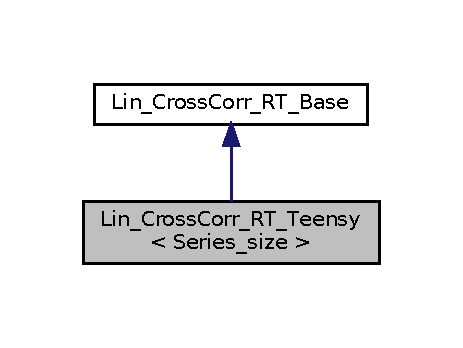
\includegraphics[width=222pt]{classLin__CrossCorr__RT__Teensy__inherit__graph}
\end{center}
\end{figure}


Collaboration diagram for Lin\+\_\+\+Cross\+Corr\+\_\+\+R\+T\+\_\+\+Teensy$<$ Series\+\_\+size $>$\+:\nopagebreak
\begin{figure}[H]
\begin{center}
\leavevmode
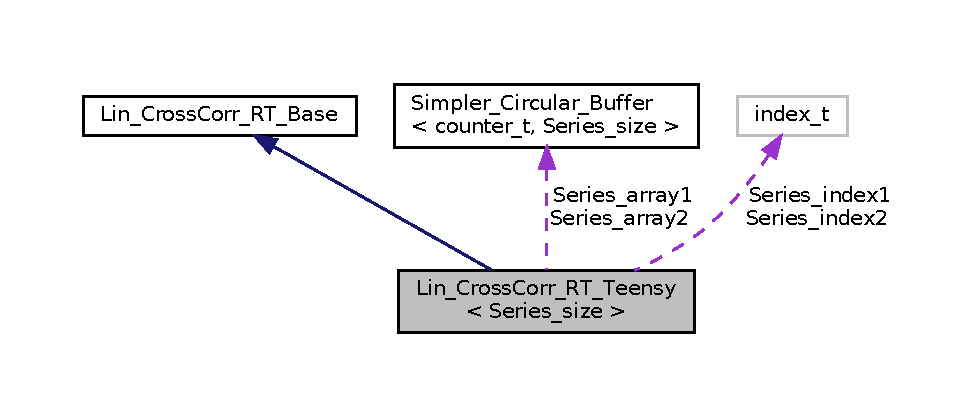
\includegraphics[width=350pt]{classLin__CrossCorr__RT__Teensy__coll__graph}
\end{center}
\end{figure}
\subsection*{Public Member Functions}
\begin{DoxyCompactItemize}
\item 
void \hyperlink{classLin__CrossCorr__RT__Teensy_a33f639fa3a6f025d5a9ebe60b969cc55}{\+\_\+\+\_\+attribute\+\_\+\+\_\+} ((flatten)) push\+\_\+datum(\hyperlink{types_8hpp_a22f279793847eba127de149437848c48}{counter\+\_\+t} datum1
\begin{DoxyCompactList}\small\item\em Stores the last active index → Post-\/increment. \end{DoxyCompactList}\item 
\hyperlink{classLin__CrossCorr__RT__Teensy_a509bcfdab5a3239a014f5805c388172a}{Series\+\_\+array2} \hyperlink{classLin__CrossCorr__RT__Teensy_af39e68107a612ca22a83046b10f52afb}{push\+\_\+back} (datum2)
\item 
\hyperlink{classLin__CrossCorr__RT__Teensy_aca7ed016d12272211206139cd120b359}{for} (unsigned int i=0;i$<$=Series\+\_\+size;i++)
\item 
void \hyperlink{classLin__CrossCorr__RT__Teensy_a1d3a4042f89c99d3705f50666fa7735c}{\+\_\+\+\_\+attribute\+\_\+\+\_\+} ((flatten)) push\+\_\+data(const \hyperlink{types_8hpp_a22f279793847eba127de149437848c48}{counter\+\_\+t} $\ast$container1
\end{DoxyCompactItemize}
\subsection*{Public Attributes}
\begin{DoxyCompactItemize}
\item 
\hyperlink{types_8hpp_a22f279793847eba127de149437848c48}{counter\+\_\+t} \hyperlink{classLin__CrossCorr__RT__Teensy_ad1a3471c7cbcee3bd9b800571cd2ae3d}{Channel\+\_\+array12} \mbox{[}Series\+\_\+size\mbox{]} = \{0\}
\item 
\hyperlink{types_8hpp_a22f279793847eba127de149437848c48}{counter\+\_\+t} \hyperlink{classLin__CrossCorr__RT__Teensy_a03a339977779908684cba60c8d3f9738}{Channel\+\_\+array21} \mbox{[}Series\+\_\+size\mbox{]} = \{0\}
\begin{DoxyCompactList}\small\item\em Stores the Channel output -\/ 12. \end{DoxyCompactList}\item 
\hyperlink{classSimpler__Circular__Buffer}{Simpler\+\_\+\+Circular\+\_\+\+Buffer}$<$ \hyperlink{types_8hpp_a22f279793847eba127de149437848c48}{counter\+\_\+t}, Series\+\_\+size $>$ \hyperlink{classLin__CrossCorr__RT__Teensy_a13307ad04080703e9ef8c0cd9794a6b0}{Series\+\_\+array1}
\begin{DoxyCompactList}\small\item\em Stores the Channel output -\/ 21. \end{DoxyCompactList}\item 
\hyperlink{classSimpler__Circular__Buffer}{Simpler\+\_\+\+Circular\+\_\+\+Buffer}$<$ \hyperlink{types_8hpp_a22f279793847eba127de149437848c48}{counter\+\_\+t}, Series\+\_\+size $>$ \hyperlink{classLin__CrossCorr__RT__Teensy_a509bcfdab5a3239a014f5805c388172a}{Series\+\_\+array2}
\item 
\hyperlink{types_8hpp_ab41b824af8e088d090c0b9e60f536c9d}{index\+\_\+t} \hyperlink{classLin__CrossCorr__RT__Teensy_afcf9512277d8bd2183ae44b8da1096df}{Series\+\_\+index1} = 0
\item 
\hyperlink{types_8hpp_ab41b824af8e088d090c0b9e60f536c9d}{index\+\_\+t} \hyperlink{classLin__CrossCorr__RT__Teensy_a945eda00978a28dd536e58e225821af6}{Series\+\_\+index2} = 0
\begin{DoxyCompactList}\small\item\em Stores the last active index → Post-\/increment. \end{DoxyCompactList}\item 
void \hyperlink{types_8hpp_a22f279793847eba127de149437848c48}{counter\+\_\+t} datum2 \hyperlink{classLin__CrossCorr__RT__Teensy_a5baab98aab70338799de9f82e7c7cc06}{override}
\item 
\hyperlink{classLin__CrossCorr__RT__Teensy_abefa188b0d61b97e915849fa8d11cc9f}{Series\+\_\+index1}
\item 
\hyperlink{classLin__CrossCorr__RT__Teensy_a4f84a456a7d6e90e8676e4c5ed059776}{Series\+\_\+index2}
\item 
void const \hyperlink{types_8hpp_a22f279793847eba127de149437848c48}{counter\+\_\+t} $\ast$ \hyperlink{classLin__CrossCorr__RT__Teensy_a9c49e09d3817e1f1344c51928e3afb57}{container2}
\end{DoxyCompactItemize}


\subsection{Detailed Description}
\subsubsection*{template$<$index\+\_\+t Series\+\_\+size$>$\newline
class Lin\+\_\+\+Cross\+Corr\+\_\+\+R\+T\+\_\+\+Teensy$<$ Series\+\_\+size $>$}

This is an implementation of Lin\+\_\+\+A\+Corr\+\_\+\+R\+T\+\_\+\+Base for Teensy with {\bfseries }(No normalisation or baseline subtraction.) 

\begin{DoxyNote}{Note}
\{ Template parameter -\/ Size of the Series and Channel array and indicates the maximum points that can be stored by the correlator object. The circuular buffer will then rewrite the older points to accomodate for the other points. \} 
\end{DoxyNote}


\subsection{Member Function Documentation}
\mbox{\Hypertarget{classLin__CrossCorr__RT__Teensy_a33f639fa3a6f025d5a9ebe60b969cc55}\label{classLin__CrossCorr__RT__Teensy_a33f639fa3a6f025d5a9ebe60b969cc55}} 
\index{Lin\+\_\+\+Cross\+Corr\+\_\+\+R\+T\+\_\+\+Teensy@{Lin\+\_\+\+Cross\+Corr\+\_\+\+R\+T\+\_\+\+Teensy}!\+\_\+\+\_\+attribute\+\_\+\+\_\+@{\+\_\+\+\_\+attribute\+\_\+\+\_\+}}
\index{\+\_\+\+\_\+attribute\+\_\+\+\_\+@{\+\_\+\+\_\+attribute\+\_\+\+\_\+}!Lin\+\_\+\+Cross\+Corr\+\_\+\+R\+T\+\_\+\+Teensy@{Lin\+\_\+\+Cross\+Corr\+\_\+\+R\+T\+\_\+\+Teensy}}
\subsubsection{\texorpdfstring{\+\_\+\+\_\+attribute\+\_\+\+\_\+()}{\_\_attribute\_\_()}\hspace{0.1cm}{\footnotesize\ttfamily [1/2]}}
{\footnotesize\ttfamily template$<$index\+\_\+t Series\+\_\+size$>$ \\
void \hyperlink{classLin__CrossCorr__RT__Teensy}{Lin\+\_\+\+Cross\+Corr\+\_\+\+R\+T\+\_\+\+Teensy}$<$ Series\+\_\+size $>$\+::\+\_\+\+\_\+attribute\+\_\+\+\_\+ (\begin{DoxyParamCaption}\item[{(flatten)}]{ }\end{DoxyParamCaption})}



Stores the last active index → Post-\/increment. 

\mbox{\Hypertarget{classLin__CrossCorr__RT__Teensy_a1d3a4042f89c99d3705f50666fa7735c}\label{classLin__CrossCorr__RT__Teensy_a1d3a4042f89c99d3705f50666fa7735c}} 
\index{Lin\+\_\+\+Cross\+Corr\+\_\+\+R\+T\+\_\+\+Teensy@{Lin\+\_\+\+Cross\+Corr\+\_\+\+R\+T\+\_\+\+Teensy}!\+\_\+\+\_\+attribute\+\_\+\+\_\+@{\+\_\+\+\_\+attribute\+\_\+\+\_\+}}
\index{\+\_\+\+\_\+attribute\+\_\+\+\_\+@{\+\_\+\+\_\+attribute\+\_\+\+\_\+}!Lin\+\_\+\+Cross\+Corr\+\_\+\+R\+T\+\_\+\+Teensy@{Lin\+\_\+\+Cross\+Corr\+\_\+\+R\+T\+\_\+\+Teensy}}
\subsubsection{\texorpdfstring{\+\_\+\+\_\+attribute\+\_\+\+\_\+()}{\_\_attribute\_\_()}\hspace{0.1cm}{\footnotesize\ttfamily [2/2]}}
{\footnotesize\ttfamily template$<$index\+\_\+t Series\+\_\+size$>$ \\
void \hyperlink{classLin__CrossCorr__RT__Teensy}{Lin\+\_\+\+Cross\+Corr\+\_\+\+R\+T\+\_\+\+Teensy}$<$ Series\+\_\+size $>$\+::\+\_\+\+\_\+attribute\+\_\+\+\_\+ (\begin{DoxyParamCaption}\item[{(flatten)}]{ }\end{DoxyParamCaption}) const}

\mbox{\Hypertarget{classLin__CrossCorr__RT__Teensy_aca7ed016d12272211206139cd120b359}\label{classLin__CrossCorr__RT__Teensy_aca7ed016d12272211206139cd120b359}} 
\index{Lin\+\_\+\+Cross\+Corr\+\_\+\+R\+T\+\_\+\+Teensy@{Lin\+\_\+\+Cross\+Corr\+\_\+\+R\+T\+\_\+\+Teensy}!for@{for}}
\index{for@{for}!Lin\+\_\+\+Cross\+Corr\+\_\+\+R\+T\+\_\+\+Teensy@{Lin\+\_\+\+Cross\+Corr\+\_\+\+R\+T\+\_\+\+Teensy}}
\subsubsection{\texorpdfstring{for()}{for()}}
{\footnotesize\ttfamily template$<$index\+\_\+t Series\+\_\+size$>$ \\
\hyperlink{classLin__CrossCorr__RT__Teensy}{Lin\+\_\+\+Cross\+Corr\+\_\+\+R\+T\+\_\+\+Teensy}$<$ Series\+\_\+size $>$\+::for (\begin{DoxyParamCaption}\item[{unsigned int}]{i = {\ttfamily 0;~i~$<$=~Series\+\_\+size;~i++} }\end{DoxyParamCaption})\hspace{0.3cm}{\ttfamily [inline]}}

\mbox{\Hypertarget{classLin__CrossCorr__RT__Teensy_af39e68107a612ca22a83046b10f52afb}\label{classLin__CrossCorr__RT__Teensy_af39e68107a612ca22a83046b10f52afb}} 
\index{Lin\+\_\+\+Cross\+Corr\+\_\+\+R\+T\+\_\+\+Teensy@{Lin\+\_\+\+Cross\+Corr\+\_\+\+R\+T\+\_\+\+Teensy}!push\+\_\+back@{push\+\_\+back}}
\index{push\+\_\+back@{push\+\_\+back}!Lin\+\_\+\+Cross\+Corr\+\_\+\+R\+T\+\_\+\+Teensy@{Lin\+\_\+\+Cross\+Corr\+\_\+\+R\+T\+\_\+\+Teensy}}
\subsubsection{\texorpdfstring{push\+\_\+back()}{push\_back()}}
{\footnotesize\ttfamily template$<$index\+\_\+t Series\+\_\+size$>$ \\
\hyperlink{classLin__CrossCorr__RT__Teensy_a509bcfdab5a3239a014f5805c388172a}{Series\+\_\+array2} \hyperlink{classLin__CrossCorr__RT__Teensy}{Lin\+\_\+\+Cross\+Corr\+\_\+\+R\+T\+\_\+\+Teensy}$<$ Series\+\_\+size $>$\+::push\+\_\+back (\begin{DoxyParamCaption}\item[{datum2}]{ }\end{DoxyParamCaption})}



\subsection{Member Data Documentation}
\mbox{\Hypertarget{classLin__CrossCorr__RT__Teensy_ad1a3471c7cbcee3bd9b800571cd2ae3d}\label{classLin__CrossCorr__RT__Teensy_ad1a3471c7cbcee3bd9b800571cd2ae3d}} 
\index{Lin\+\_\+\+Cross\+Corr\+\_\+\+R\+T\+\_\+\+Teensy@{Lin\+\_\+\+Cross\+Corr\+\_\+\+R\+T\+\_\+\+Teensy}!Channel\+\_\+array12@{Channel\+\_\+array12}}
\index{Channel\+\_\+array12@{Channel\+\_\+array12}!Lin\+\_\+\+Cross\+Corr\+\_\+\+R\+T\+\_\+\+Teensy@{Lin\+\_\+\+Cross\+Corr\+\_\+\+R\+T\+\_\+\+Teensy}}
\subsubsection{\texorpdfstring{Channel\+\_\+array12}{Channel\_array12}}
{\footnotesize\ttfamily template$<$index\+\_\+t Series\+\_\+size$>$ \\
\hyperlink{types_8hpp_a22f279793847eba127de149437848c48}{counter\+\_\+t} \hyperlink{classLin__CrossCorr__RT__Teensy}{Lin\+\_\+\+Cross\+Corr\+\_\+\+R\+T\+\_\+\+Teensy}$<$ Series\+\_\+size $>$\+::Channel\+\_\+array12\mbox{[}Series\+\_\+size\mbox{]} = \{0\}}

\mbox{\Hypertarget{classLin__CrossCorr__RT__Teensy_a03a339977779908684cba60c8d3f9738}\label{classLin__CrossCorr__RT__Teensy_a03a339977779908684cba60c8d3f9738}} 
\index{Lin\+\_\+\+Cross\+Corr\+\_\+\+R\+T\+\_\+\+Teensy@{Lin\+\_\+\+Cross\+Corr\+\_\+\+R\+T\+\_\+\+Teensy}!Channel\+\_\+array21@{Channel\+\_\+array21}}
\index{Channel\+\_\+array21@{Channel\+\_\+array21}!Lin\+\_\+\+Cross\+Corr\+\_\+\+R\+T\+\_\+\+Teensy@{Lin\+\_\+\+Cross\+Corr\+\_\+\+R\+T\+\_\+\+Teensy}}
\subsubsection{\texorpdfstring{Channel\+\_\+array21}{Channel\_array21}}
{\footnotesize\ttfamily template$<$index\+\_\+t Series\+\_\+size$>$ \\
\hyperlink{types_8hpp_a22f279793847eba127de149437848c48}{counter\+\_\+t} \hyperlink{classLin__CrossCorr__RT__Teensy}{Lin\+\_\+\+Cross\+Corr\+\_\+\+R\+T\+\_\+\+Teensy}$<$ Series\+\_\+size $>$\+::Channel\+\_\+array21\mbox{[}Series\+\_\+size\mbox{]} = \{0\}}



Stores the Channel output -\/ 12. 

\mbox{\Hypertarget{classLin__CrossCorr__RT__Teensy_a9c49e09d3817e1f1344c51928e3afb57}\label{classLin__CrossCorr__RT__Teensy_a9c49e09d3817e1f1344c51928e3afb57}} 
\index{Lin\+\_\+\+Cross\+Corr\+\_\+\+R\+T\+\_\+\+Teensy@{Lin\+\_\+\+Cross\+Corr\+\_\+\+R\+T\+\_\+\+Teensy}!container2@{container2}}
\index{container2@{container2}!Lin\+\_\+\+Cross\+Corr\+\_\+\+R\+T\+\_\+\+Teensy@{Lin\+\_\+\+Cross\+Corr\+\_\+\+R\+T\+\_\+\+Teensy}}
\subsubsection{\texorpdfstring{container2}{container2}}
{\footnotesize\ttfamily template$<$index\+\_\+t Series\+\_\+size$>$ \\
void const \hyperlink{types_8hpp_a22f279793847eba127de149437848c48}{counter\+\_\+t}$\ast$ \hyperlink{classLin__CrossCorr__RT__Teensy}{Lin\+\_\+\+Cross\+Corr\+\_\+\+R\+T\+\_\+\+Teensy}$<$ Series\+\_\+size $>$\+::container2}

\mbox{\Hypertarget{classLin__CrossCorr__RT__Teensy_a5baab98aab70338799de9f82e7c7cc06}\label{classLin__CrossCorr__RT__Teensy_a5baab98aab70338799de9f82e7c7cc06}} 
\index{Lin\+\_\+\+Cross\+Corr\+\_\+\+R\+T\+\_\+\+Teensy@{Lin\+\_\+\+Cross\+Corr\+\_\+\+R\+T\+\_\+\+Teensy}!override@{override}}
\index{override@{override}!Lin\+\_\+\+Cross\+Corr\+\_\+\+R\+T\+\_\+\+Teensy@{Lin\+\_\+\+Cross\+Corr\+\_\+\+R\+T\+\_\+\+Teensy}}
\subsubsection{\texorpdfstring{override}{override}}
{\footnotesize\ttfamily template$<$index\+\_\+t Series\+\_\+size$>$ \\
void \hyperlink{types_8hpp_a22f279793847eba127de149437848c48}{counter\+\_\+t} datum2 \hyperlink{classLin__CrossCorr__RT__Teensy}{Lin\+\_\+\+Cross\+Corr\+\_\+\+R\+T\+\_\+\+Teensy}$<$ Series\+\_\+size $>$\+::override}

{\bfseries Initial value\+:}
\begin{DoxyCode}
\{
    \hyperlink{classLin__CrossCorr__RT__Teensy_a13307ad04080703e9ef8c0cd9794a6b0}{Series\_array1}.\hyperlink{classSimpler__Circular__Buffer_af4bdd0a6d3fc7a8c06f62b0d996158f0}{push\_back}(datum1)
\end{DoxyCode}
\mbox{\Hypertarget{classLin__CrossCorr__RT__Teensy_a13307ad04080703e9ef8c0cd9794a6b0}\label{classLin__CrossCorr__RT__Teensy_a13307ad04080703e9ef8c0cd9794a6b0}} 
\index{Lin\+\_\+\+Cross\+Corr\+\_\+\+R\+T\+\_\+\+Teensy@{Lin\+\_\+\+Cross\+Corr\+\_\+\+R\+T\+\_\+\+Teensy}!Series\+\_\+array1@{Series\+\_\+array1}}
\index{Series\+\_\+array1@{Series\+\_\+array1}!Lin\+\_\+\+Cross\+Corr\+\_\+\+R\+T\+\_\+\+Teensy@{Lin\+\_\+\+Cross\+Corr\+\_\+\+R\+T\+\_\+\+Teensy}}
\subsubsection{\texorpdfstring{Series\+\_\+array1}{Series\_array1}}
{\footnotesize\ttfamily template$<$index\+\_\+t Series\+\_\+size$>$ \\
\hyperlink{classSimpler__Circular__Buffer}{Simpler\+\_\+\+Circular\+\_\+\+Buffer}$<$\hyperlink{types_8hpp_a22f279793847eba127de149437848c48}{counter\+\_\+t}, Series\+\_\+size$>$ \hyperlink{classLin__CrossCorr__RT__Teensy}{Lin\+\_\+\+Cross\+Corr\+\_\+\+R\+T\+\_\+\+Teensy}$<$ Series\+\_\+size $>$\+::Series\+\_\+array1}



Stores the Channel output -\/ 21. 

Stores the data points in a circular Buffer \mbox{\Hypertarget{classLin__CrossCorr__RT__Teensy_a509bcfdab5a3239a014f5805c388172a}\label{classLin__CrossCorr__RT__Teensy_a509bcfdab5a3239a014f5805c388172a}} 
\index{Lin\+\_\+\+Cross\+Corr\+\_\+\+R\+T\+\_\+\+Teensy@{Lin\+\_\+\+Cross\+Corr\+\_\+\+R\+T\+\_\+\+Teensy}!Series\+\_\+array2@{Series\+\_\+array2}}
\index{Series\+\_\+array2@{Series\+\_\+array2}!Lin\+\_\+\+Cross\+Corr\+\_\+\+R\+T\+\_\+\+Teensy@{Lin\+\_\+\+Cross\+Corr\+\_\+\+R\+T\+\_\+\+Teensy}}
\subsubsection{\texorpdfstring{Series\+\_\+array2}{Series\_array2}}
{\footnotesize\ttfamily template$<$index\+\_\+t Series\+\_\+size$>$ \\
\hyperlink{classSimpler__Circular__Buffer}{Simpler\+\_\+\+Circular\+\_\+\+Buffer}$<$\hyperlink{types_8hpp_a22f279793847eba127de149437848c48}{counter\+\_\+t}, Series\+\_\+size$>$ \hyperlink{classLin__CrossCorr__RT__Teensy}{Lin\+\_\+\+Cross\+Corr\+\_\+\+R\+T\+\_\+\+Teensy}$<$ Series\+\_\+size $>$\+::Series\+\_\+array2}

\mbox{\Hypertarget{classLin__CrossCorr__RT__Teensy_afcf9512277d8bd2183ae44b8da1096df}\label{classLin__CrossCorr__RT__Teensy_afcf9512277d8bd2183ae44b8da1096df}} 
\index{Lin\+\_\+\+Cross\+Corr\+\_\+\+R\+T\+\_\+\+Teensy@{Lin\+\_\+\+Cross\+Corr\+\_\+\+R\+T\+\_\+\+Teensy}!Series\+\_\+index1@{Series\+\_\+index1}}
\index{Series\+\_\+index1@{Series\+\_\+index1}!Lin\+\_\+\+Cross\+Corr\+\_\+\+R\+T\+\_\+\+Teensy@{Lin\+\_\+\+Cross\+Corr\+\_\+\+R\+T\+\_\+\+Teensy}}
\subsubsection{\texorpdfstring{Series\+\_\+index1}{Series\_index1}\hspace{0.1cm}{\footnotesize\ttfamily [1/2]}}
{\footnotesize\ttfamily template$<$index\+\_\+t Series\+\_\+size$>$ \\
\hyperlink{types_8hpp_ab41b824af8e088d090c0b9e60f536c9d}{index\+\_\+t} \hyperlink{classLin__CrossCorr__RT__Teensy}{Lin\+\_\+\+Cross\+Corr\+\_\+\+R\+T\+\_\+\+Teensy}$<$ Series\+\_\+size $>$\+::Series\+\_\+index1 = 0}

\mbox{\Hypertarget{classLin__CrossCorr__RT__Teensy_abefa188b0d61b97e915849fa8d11cc9f}\label{classLin__CrossCorr__RT__Teensy_abefa188b0d61b97e915849fa8d11cc9f}} 
\index{Lin\+\_\+\+Cross\+Corr\+\_\+\+R\+T\+\_\+\+Teensy@{Lin\+\_\+\+Cross\+Corr\+\_\+\+R\+T\+\_\+\+Teensy}!Series\+\_\+index1@{Series\+\_\+index1}}
\index{Series\+\_\+index1@{Series\+\_\+index1}!Lin\+\_\+\+Cross\+Corr\+\_\+\+R\+T\+\_\+\+Teensy@{Lin\+\_\+\+Cross\+Corr\+\_\+\+R\+T\+\_\+\+Teensy}}
\subsubsection{\texorpdfstring{Series\+\_\+index1}{Series\_index1}\hspace{0.1cm}{\footnotesize\ttfamily [2/2]}}
{\footnotesize\ttfamily template$<$index\+\_\+t Series\+\_\+size$>$ \\
\hyperlink{classLin__CrossCorr__RT__Teensy}{Lin\+\_\+\+Cross\+Corr\+\_\+\+R\+T\+\_\+\+Teensy}$<$ Series\+\_\+size $>$\+::Series\+\_\+index1}

\mbox{\Hypertarget{classLin__CrossCorr__RT__Teensy_a945eda00978a28dd536e58e225821af6}\label{classLin__CrossCorr__RT__Teensy_a945eda00978a28dd536e58e225821af6}} 
\index{Lin\+\_\+\+Cross\+Corr\+\_\+\+R\+T\+\_\+\+Teensy@{Lin\+\_\+\+Cross\+Corr\+\_\+\+R\+T\+\_\+\+Teensy}!Series\+\_\+index2@{Series\+\_\+index2}}
\index{Series\+\_\+index2@{Series\+\_\+index2}!Lin\+\_\+\+Cross\+Corr\+\_\+\+R\+T\+\_\+\+Teensy@{Lin\+\_\+\+Cross\+Corr\+\_\+\+R\+T\+\_\+\+Teensy}}
\subsubsection{\texorpdfstring{Series\+\_\+index2}{Series\_index2}\hspace{0.1cm}{\footnotesize\ttfamily [1/2]}}
{\footnotesize\ttfamily template$<$index\+\_\+t Series\+\_\+size$>$ \\
\hyperlink{types_8hpp_ab41b824af8e088d090c0b9e60f536c9d}{index\+\_\+t} \hyperlink{classLin__CrossCorr__RT__Teensy}{Lin\+\_\+\+Cross\+Corr\+\_\+\+R\+T\+\_\+\+Teensy}$<$ Series\+\_\+size $>$\+::Series\+\_\+index2 = 0}



Stores the last active index → Post-\/increment. 

\mbox{\Hypertarget{classLin__CrossCorr__RT__Teensy_a4f84a456a7d6e90e8676e4c5ed059776}\label{classLin__CrossCorr__RT__Teensy_a4f84a456a7d6e90e8676e4c5ed059776}} 
\index{Lin\+\_\+\+Cross\+Corr\+\_\+\+R\+T\+\_\+\+Teensy@{Lin\+\_\+\+Cross\+Corr\+\_\+\+R\+T\+\_\+\+Teensy}!Series\+\_\+index2@{Series\+\_\+index2}}
\index{Series\+\_\+index2@{Series\+\_\+index2}!Lin\+\_\+\+Cross\+Corr\+\_\+\+R\+T\+\_\+\+Teensy@{Lin\+\_\+\+Cross\+Corr\+\_\+\+R\+T\+\_\+\+Teensy}}
\subsubsection{\texorpdfstring{Series\+\_\+index2}{Series\_index2}\hspace{0.1cm}{\footnotesize\ttfamily [2/2]}}
{\footnotesize\ttfamily template$<$index\+\_\+t Series\+\_\+size$>$ \\
\hyperlink{classLin__CrossCorr__RT__Teensy}{Lin\+\_\+\+Cross\+Corr\+\_\+\+R\+T\+\_\+\+Teensy}$<$ Series\+\_\+size $>$\+::Series\+\_\+index2}



The documentation for this class was generated from the following file\+:\begin{DoxyCompactItemize}
\item 
code/software/\hyperlink{Lin__CrossCorr__RT__Teensy_8hpp}{Lin\+\_\+\+Cross\+Corr\+\_\+\+R\+T\+\_\+\+Teensy.\+hpp}\end{DoxyCompactItemize}

\hypertarget{classLinACorrRTTeensy}{}\section{Lin\+A\+Corr\+R\+T\+Teensy$<$ Series\+\_\+\+Size, has\+Monitor\+Channel $>$ Class Template Reference}
\label{classLinACorrRTTeensy}\index{Lin\+A\+Corr\+R\+T\+Teensy$<$ Series\+\_\+\+Size, has\+Monitor\+Channel $>$@{Lin\+A\+Corr\+R\+T\+Teensy$<$ Series\+\_\+\+Size, has\+Monitor\+Channel $>$}}


This is an implementation of Lin\+\_\+\+A\+Corr\+\_\+\+R\+T\+\_\+\+Base for Teensy with {\bfseries }(No normalisation or baseline subtraction.)  




{\ttfamily \#include $<$Lin\+\_\+\+A\+Corr\+\_\+\+R\+T\+\_\+\+Teensy.\+hpp$>$}



Collaboration diagram for Lin\+A\+Corr\+R\+T\+Teensy$<$ Series\+\_\+\+Size, has\+Monitor\+Channel $>$\+:
\nopagebreak
\begin{figure}[H]
\begin{center}
\leavevmode
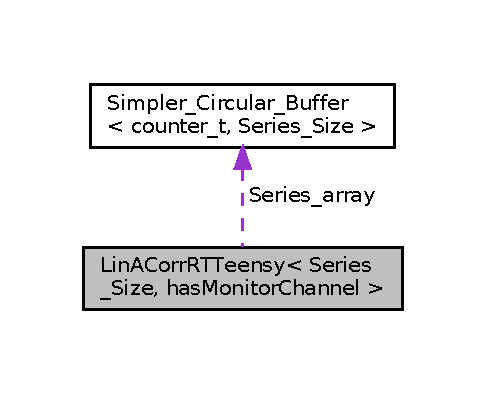
\includegraphics[width=233pt]{classLinACorrRTTeensy__coll__graph}
\end{center}
\end{figure}
\subsection*{Public Member Functions}
\begin{DoxyCompactItemize}
\item 
\hyperlink{classLinACorrRTTeensy_aebb83829899235fe5177de735a5367da}{Lin\+A\+Corr\+R\+T\+Teensy} ()
\begin{DoxyCompactList}\small\item\em Default Constructor. \end{DoxyCompactList}\item 
void \hyperlink{classLinACorrRTTeensy_aacc634aad2252efbb6ee3a4c2ac422dc}{push\+\_\+datum} (\hyperlink{types_8hpp_a22f279793847eba127de149437848c48}{counter\+\_\+t} datum)
\begin{DoxyCompactList}\small\item\em Adds new {\itshape single} data point and processes it to the {\ttfamily Channel}. \end{DoxyCompactList}\item 
void \hyperlink{classLinACorrRTTeensy_abf6a40dff92088469fbb8ceabf9da799}{push\+\_\+data} (const \hyperlink{types_8hpp_a22f279793847eba127de149437848c48}{counter\+\_\+t} $\ast$container, const \hyperlink{types_8hpp_a7c40bb931c31595ed6308605f4537447}{index\+\_\+t} size) \+\_\+\+\_\+attribute\+\_\+\+\_\+((flatten))
\begin{DoxyCompactList}\small\item\em Repeatedly calls {\ttfamily \hyperlink{classLinACorrRTTeensy_aacc634aad2252efbb6ee3a4c2ac422dc}{push\+\_\+datum()}} on the given container of values, one at a time. \end{DoxyCompactList}\item 
float\+\_\+t \hyperlink{classLinACorrRTTeensy_a98110e3b97a2300b9078a6e57a8234bc}{norm} ()
\begin{DoxyCompactList}\small\item\em Returns the accumulate of the channel so far. \end{DoxyCompactList}\item 
void \hyperlink{classLinACorrRTTeensy_a967f1b3ea7e6ebdae8c9bf7c2c641e49}{ch\+\_\+out} () const \+\_\+\+\_\+attribute\+\_\+\+\_\+((always\+\_\+inline))
\begin{DoxyCompactList}\small\item\em Outputs the complete channel to the Serial port. \end{DoxyCompactList}\item 
void \hyperlink{classLinACorrRTTeensy_a4d1be65472a058b056386286d093b847}{ch\+\_\+out\+\_\+norm} () const \+\_\+\+\_\+attribute\+\_\+\+\_\+((flatten))
\begin{DoxyCompactList}\small\item\em Outputs the channel array to the Serial port after normalising it. \end{DoxyCompactList}\end{DoxyCompactItemize}
\subsection*{Public Attributes}
\begin{DoxyCompactItemize}
\item 
channel\+\_\+t \hyperlink{classLinACorrRTTeensy_a3276cb9bb215af9676edc35958c889b8}{Channel\+\_\+array} \mbox{[}Series\+\_\+\+Size\mbox{]} = \{0\}
\begin{DoxyCompactList}\small\item\em Defines a run-\/time polymorphic \hyperlink{classMonitorChannel}{Monitor\+Channel} object, which decomposes to {\ttfamily ghost} channel (Unit\+Mean\+Channel) if {\ttfamily has\+Monitor\+Channel} is true. Basically {\ttfamily Unit\+Mean\+Channel} does nothing. \end{DoxyCompactList}\item 
\hyperlink{classSimpler__Circular__Buffer}{Simpler\+\_\+\+Circular\+\_\+\+Buffer}$<$ \hyperlink{types_8hpp_a22f279793847eba127de149437848c48}{counter\+\_\+t}, Series\+\_\+\+Size $>$ \hyperlink{classLinACorrRTTeensy_a5c4cc1fe032812d6290579c7c8b22e57}{Series\+\_\+array}
\begin{DoxyCompactList}\small\item\em Stores the data points in a circular Buffer. \end{DoxyCompactList}\item 
\hyperlink{types_8hpp_a7c40bb931c31595ed6308605f4537447}{index\+\_\+t} \hyperlink{classLinACorrRTTeensy_abe0523ada55375281deacb143b6055b7}{Series\+\_\+index} = 0
\begin{DoxyCompactList}\small\item\em Stores the last active index → Post-\/increment. \end{DoxyCompactList}\end{DoxyCompactItemize}


\subsection{Detailed Description}
\subsubsection*{template$<$index\+\_\+t Series\+\_\+\+Size, bool has\+Monitor\+Channel$>$\newline
class Lin\+A\+Corr\+R\+T\+Teensy$<$ Series\+\_\+\+Size, has\+Monitor\+Channel $>$}

This is an implementation of Lin\+\_\+\+A\+Corr\+\_\+\+R\+T\+\_\+\+Base for Teensy with {\bfseries }(No normalisation or baseline subtraction.) 

\begin{DoxyNote}{Note}
\{ Template parameter -\/ Size of the Series and Channel array and indicates the maximum points that can be stored by the correlator object. The circuular buffer will then rewrite the older points to accomodate for the other points. \} 
\end{DoxyNote}


\subsection{Constructor \& Destructor Documentation}
\mbox{\Hypertarget{classLinACorrRTTeensy_aebb83829899235fe5177de735a5367da}\label{classLinACorrRTTeensy_aebb83829899235fe5177de735a5367da}} 
\index{Lin\+A\+Corr\+R\+T\+Teensy@{Lin\+A\+Corr\+R\+T\+Teensy}!Lin\+A\+Corr\+R\+T\+Teensy@{Lin\+A\+Corr\+R\+T\+Teensy}}
\index{Lin\+A\+Corr\+R\+T\+Teensy@{Lin\+A\+Corr\+R\+T\+Teensy}!Lin\+A\+Corr\+R\+T\+Teensy@{Lin\+A\+Corr\+R\+T\+Teensy}}
\subsubsection{\texorpdfstring{Lin\+A\+Corr\+R\+T\+Teensy()}{LinACorrRTTeensy()}}
{\footnotesize\ttfamily template$<$index\+\_\+t Series\+\_\+\+Size, bool has\+Monitor\+Channel$>$ \\
\hyperlink{classLinACorrRTTeensy}{Lin\+A\+Corr\+R\+T\+Teensy}$<$ Series\+\_\+\+Size, has\+Monitor\+Channel $>$\+::\hyperlink{classLinACorrRTTeensy}{Lin\+A\+Corr\+R\+T\+Teensy} (\begin{DoxyParamCaption}{ }\end{DoxyParamCaption})\hspace{0.3cm}{\ttfamily [inline]}}



Default Constructor. 



\subsection{Member Function Documentation}
\mbox{\Hypertarget{classLinACorrRTTeensy_a967f1b3ea7e6ebdae8c9bf7c2c641e49}\label{classLinACorrRTTeensy_a967f1b3ea7e6ebdae8c9bf7c2c641e49}} 
\index{Lin\+A\+Corr\+R\+T\+Teensy@{Lin\+A\+Corr\+R\+T\+Teensy}!ch\+\_\+out@{ch\+\_\+out}}
\index{ch\+\_\+out@{ch\+\_\+out}!Lin\+A\+Corr\+R\+T\+Teensy@{Lin\+A\+Corr\+R\+T\+Teensy}}
\subsubsection{\texorpdfstring{ch\+\_\+out()}{ch\_out()}}
{\footnotesize\ttfamily template$<$index\+\_\+t Series\+\_\+\+Size, bool has\+Monitor\+Channel$>$ \\
void \hyperlink{classLinACorrRTTeensy}{Lin\+A\+Corr\+R\+T\+Teensy}$<$ Series\+\_\+\+Size, has\+Monitor\+Channel $>$\+::ch\+\_\+out (\begin{DoxyParamCaption}{ }\end{DoxyParamCaption}) const\hspace{0.3cm}{\ttfamily [inline]}}



Outputs the complete channel to the Serial port. 

\mbox{\Hypertarget{classLinACorrRTTeensy_a4d1be65472a058b056386286d093b847}\label{classLinACorrRTTeensy_a4d1be65472a058b056386286d093b847}} 
\index{Lin\+A\+Corr\+R\+T\+Teensy@{Lin\+A\+Corr\+R\+T\+Teensy}!ch\+\_\+out\+\_\+norm@{ch\+\_\+out\+\_\+norm}}
\index{ch\+\_\+out\+\_\+norm@{ch\+\_\+out\+\_\+norm}!Lin\+A\+Corr\+R\+T\+Teensy@{Lin\+A\+Corr\+R\+T\+Teensy}}
\subsubsection{\texorpdfstring{ch\+\_\+out\+\_\+norm()}{ch\_out\_norm()}}
{\footnotesize\ttfamily template$<$index\+\_\+t Series\+\_\+\+Size, bool has\+Monitor\+Channel$>$ \\
void \hyperlink{classLinACorrRTTeensy}{Lin\+A\+Corr\+R\+T\+Teensy}$<$ Series\+\_\+\+Size, has\+Monitor\+Channel $>$\+::ch\+\_\+out\+\_\+norm (\begin{DoxyParamCaption}{ }\end{DoxyParamCaption}) const\hspace{0.3cm}{\ttfamily [inline]}}



Outputs the channel array to the Serial port after normalising it. 

\mbox{\Hypertarget{classLinACorrRTTeensy_a98110e3b97a2300b9078a6e57a8234bc}\label{classLinACorrRTTeensy_a98110e3b97a2300b9078a6e57a8234bc}} 
\index{Lin\+A\+Corr\+R\+T\+Teensy@{Lin\+A\+Corr\+R\+T\+Teensy}!norm@{norm}}
\index{norm@{norm}!Lin\+A\+Corr\+R\+T\+Teensy@{Lin\+A\+Corr\+R\+T\+Teensy}}
\subsubsection{\texorpdfstring{norm()}{norm()}}
{\footnotesize\ttfamily template$<$index\+\_\+t Series\+\_\+\+Size, bool has\+Monitor\+Channel$>$ \\
float\+\_\+t \hyperlink{classLinACorrRTTeensy}{Lin\+A\+Corr\+R\+T\+Teensy}$<$ Series\+\_\+\+Size, has\+Monitor\+Channel $>$\+::norm (\begin{DoxyParamCaption}{ }\end{DoxyParamCaption})\hspace{0.3cm}{\ttfamily [inline]}}



Returns the accumulate of the channel so far. 


\begin{DoxyParams}{Parameters}
{\em Lag} & time that is ignored by the function. \\
\hline
\end{DoxyParams}
\mbox{\Hypertarget{classLinACorrRTTeensy_abf6a40dff92088469fbb8ceabf9da799}\label{classLinACorrRTTeensy_abf6a40dff92088469fbb8ceabf9da799}} 
\index{Lin\+A\+Corr\+R\+T\+Teensy@{Lin\+A\+Corr\+R\+T\+Teensy}!push\+\_\+data@{push\+\_\+data}}
\index{push\+\_\+data@{push\+\_\+data}!Lin\+A\+Corr\+R\+T\+Teensy@{Lin\+A\+Corr\+R\+T\+Teensy}}
\subsubsection{\texorpdfstring{push\+\_\+data()}{push\_data()}}
{\footnotesize\ttfamily template$<$index\+\_\+t Series\+\_\+\+Size, bool has\+Monitor\+Channel$>$ \\
void \hyperlink{classLinACorrRTTeensy}{Lin\+A\+Corr\+R\+T\+Teensy}$<$ Series\+\_\+\+Size, has\+Monitor\+Channel $>$\+::push\+\_\+data (\begin{DoxyParamCaption}\item[{const \hyperlink{types_8hpp_a22f279793847eba127de149437848c48}{counter\+\_\+t} $\ast$}]{container,  }\item[{const \hyperlink{types_8hpp_a7c40bb931c31595ed6308605f4537447}{index\+\_\+t}}]{size }\end{DoxyParamCaption})\hspace{0.3cm}{\ttfamily [inline]}}



Repeatedly calls {\ttfamily \hyperlink{classLinACorrRTTeensy_aacc634aad2252efbb6ee3a4c2ac422dc}{push\+\_\+datum()}} on the given container of values, one at a time. 

\mbox{\Hypertarget{classLinACorrRTTeensy_aacc634aad2252efbb6ee3a4c2ac422dc}\label{classLinACorrRTTeensy_aacc634aad2252efbb6ee3a4c2ac422dc}} 
\index{Lin\+A\+Corr\+R\+T\+Teensy@{Lin\+A\+Corr\+R\+T\+Teensy}!push\+\_\+datum@{push\+\_\+datum}}
\index{push\+\_\+datum@{push\+\_\+datum}!Lin\+A\+Corr\+R\+T\+Teensy@{Lin\+A\+Corr\+R\+T\+Teensy}}
\subsubsection{\texorpdfstring{push\+\_\+datum()}{push\_datum()}}
{\footnotesize\ttfamily template$<$index\+\_\+t Series\+\_\+\+Size, bool has\+Monitor\+Channel$>$ \\
void \hyperlink{classLinACorrRTTeensy}{Lin\+A\+Corr\+R\+T\+Teensy}$<$ Series\+\_\+\+Size, has\+Monitor\+Channel $>$\+::push\+\_\+datum (\begin{DoxyParamCaption}\item[{\hyperlink{types_8hpp_a22f279793847eba127de149437848c48}{counter\+\_\+t}}]{datum }\end{DoxyParamCaption})\hspace{0.3cm}{\ttfamily [inline]}}



Adds new {\itshape single} data point and processes it to the {\ttfamily Channel}. 



\subsection{Member Data Documentation}
\mbox{\Hypertarget{classLinACorrRTTeensy_a3276cb9bb215af9676edc35958c889b8}\label{classLinACorrRTTeensy_a3276cb9bb215af9676edc35958c889b8}} 
\index{Lin\+A\+Corr\+R\+T\+Teensy@{Lin\+A\+Corr\+R\+T\+Teensy}!Channel\+\_\+array@{Channel\+\_\+array}}
\index{Channel\+\_\+array@{Channel\+\_\+array}!Lin\+A\+Corr\+R\+T\+Teensy@{Lin\+A\+Corr\+R\+T\+Teensy}}
\subsubsection{\texorpdfstring{Channel\+\_\+array}{Channel\_array}}
{\footnotesize\ttfamily template$<$index\+\_\+t Series\+\_\+\+Size, bool has\+Monitor\+Channel$>$ \\
channel\+\_\+t \hyperlink{classLinACorrRTTeensy}{Lin\+A\+Corr\+R\+T\+Teensy}$<$ Series\+\_\+\+Size, has\+Monitor\+Channel $>$\+::Channel\+\_\+array\mbox{[}Series\+\_\+\+Size\mbox{]} = \{0\}}



Defines a run-\/time polymorphic \hyperlink{classMonitorChannel}{Monitor\+Channel} object, which decomposes to {\ttfamily ghost} channel (Unit\+Mean\+Channel) if {\ttfamily has\+Monitor\+Channel} is true. Basically {\ttfamily Unit\+Mean\+Channel} does nothing. 

Stores the Channel output \mbox{\Hypertarget{classLinACorrRTTeensy_a5c4cc1fe032812d6290579c7c8b22e57}\label{classLinACorrRTTeensy_a5c4cc1fe032812d6290579c7c8b22e57}} 
\index{Lin\+A\+Corr\+R\+T\+Teensy@{Lin\+A\+Corr\+R\+T\+Teensy}!Series\+\_\+array@{Series\+\_\+array}}
\index{Series\+\_\+array@{Series\+\_\+array}!Lin\+A\+Corr\+R\+T\+Teensy@{Lin\+A\+Corr\+R\+T\+Teensy}}
\subsubsection{\texorpdfstring{Series\+\_\+array}{Series\_array}}
{\footnotesize\ttfamily template$<$index\+\_\+t Series\+\_\+\+Size, bool has\+Monitor\+Channel$>$ \\
\hyperlink{classSimpler__Circular__Buffer}{Simpler\+\_\+\+Circular\+\_\+\+Buffer}$<$\hyperlink{types_8hpp_a22f279793847eba127de149437848c48}{counter\+\_\+t}, Series\+\_\+\+Size$>$ \hyperlink{classLinACorrRTTeensy}{Lin\+A\+Corr\+R\+T\+Teensy}$<$ Series\+\_\+\+Size, has\+Monitor\+Channel $>$\+::Series\+\_\+array}



Stores the data points in a circular Buffer. 

\mbox{\Hypertarget{classLinACorrRTTeensy_abe0523ada55375281deacb143b6055b7}\label{classLinACorrRTTeensy_abe0523ada55375281deacb143b6055b7}} 
\index{Lin\+A\+Corr\+R\+T\+Teensy@{Lin\+A\+Corr\+R\+T\+Teensy}!Series\+\_\+index@{Series\+\_\+index}}
\index{Series\+\_\+index@{Series\+\_\+index}!Lin\+A\+Corr\+R\+T\+Teensy@{Lin\+A\+Corr\+R\+T\+Teensy}}
\subsubsection{\texorpdfstring{Series\+\_\+index}{Series\_index}}
{\footnotesize\ttfamily template$<$index\+\_\+t Series\+\_\+\+Size, bool has\+Monitor\+Channel$>$ \\
\hyperlink{types_8hpp_a7c40bb931c31595ed6308605f4537447}{index\+\_\+t} \hyperlink{classLinACorrRTTeensy}{Lin\+A\+Corr\+R\+T\+Teensy}$<$ Series\+\_\+\+Size, has\+Monitor\+Channel $>$\+::Series\+\_\+index = 0}



Stores the last active index → Post-\/increment. 



The documentation for this class was generated from the following file\+:\begin{DoxyCompactItemize}
\item 
code/software/\hyperlink{Lin__ACorr__RT__Teensy_8hpp}{Lin\+\_\+\+A\+Corr\+\_\+\+R\+T\+\_\+\+Teensy.\+hpp}\end{DoxyCompactItemize}

\hypertarget{classMonitorChannel}{}\section{Monitor\+Channel$<$ Mean\+Channel $>$ Class Template Reference}
\label{classMonitorChannel}\index{Monitor\+Channel$<$ Mean\+Channel $>$@{Monitor\+Channel$<$ Mean\+Channel $>$}}


A simple Averager Class that calculates the estimated mean. Template parameter {\ttfamily Construct} specifies a template specialization that either constructs a functional object when it is {\ttfamily true} or constructs a near zerp-\/signature {\bfseries dummy object} when set to {\ttfamily false}.  




{\ttfamily \#include $<$monitor\+\_\+channel.\+hpp$>$}



\subsection{Detailed Description}
\subsubsection*{template$<$bool Mean\+Channel = true$>$\newline
class Monitor\+Channel$<$ Mean\+Channel $>$}

A simple Averager Class that calculates the estimated mean. Template parameter {\ttfamily Construct} specifies a template specialization that either constructs a functional object when it is {\ttfamily true} or constructs a near zerp-\/signature {\bfseries dummy object} when set to {\ttfamily false}. 

The documentation for this class was generated from the following file\+:\begin{DoxyCompactItemize}
\item 
code/software/\hyperlink{monitor__channel_8hpp}{monitor\+\_\+channel.\+hpp}\end{DoxyCompactItemize}

\hypertarget{classMonitorChannel_3_01false_01_4}{}\section{Monitor\+Channel$<$ false $>$ Class Template Reference}
\label{classMonitorChannel_3_01false_01_4}\index{Monitor\+Channel$<$ false $>$@{Monitor\+Channel$<$ false $>$}}


Specialization -\/$>$ Counter Monitor (degenerated mean monitor).  




{\ttfamily \#include $<$monitor\+\_\+channel.\+hpp$>$}



Collaboration diagram for Monitor\+Channel$<$ false $>$\+:
\nopagebreak
\begin{figure}[H]
\begin{center}
\leavevmode
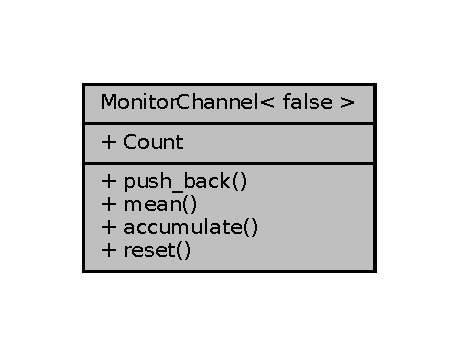
\includegraphics[width=220pt]{d0/de8/classMonitorChannel_3_01false_01_4__coll__graph}
\end{center}
\end{figure}
\subsection*{Public Types}
\begin{DoxyCompactItemize}
\item 
using \hyperlink{classMonitorChannel_3_01false_01_4_a72d6a503399e9e8e986f0258d508a1b2}{Accumulate\+Type} = uint32\+\_\+t
\end{DoxyCompactItemize}
\subsection*{Public Member Functions}
\begin{DoxyCompactItemize}
\item 
void \hyperlink{classMonitorChannel_3_01false_01_4_aec5ccac7dbda7816b5ddc163d6d4aa5b}{push\+\_\+back} () \+\_\+\+\_\+attribute\+\_\+\+\_\+((always\+\_\+inline))
\item 
float\+\_\+t \hyperlink{classMonitorChannel_3_01false_01_4_aff1c900b36c53bd674b53f94c3c2770b}{mean} () const \+\_\+\+\_\+attribute\+\_\+\+\_\+((always\+\_\+inline))
\item 
\hyperlink{classMonitorChannel_3_01false_01_4_a72d6a503399e9e8e986f0258d508a1b2}{Accumulate\+Type} \hyperlink{classMonitorChannel_3_01false_01_4_a55677fe669bca6b9382fc3baa73162b9}{accumulate} () const \+\_\+\+\_\+attribute\+\_\+\+\_\+((always\+\_\+inline))
\begin{DoxyCompactList}\small\item\em Returns the accumulate so far, which is the same as \textquotesingle{}Count`. \end{DoxyCompactList}\item 
void \hyperlink{classMonitorChannel_3_01false_01_4_a9310343e280b593894ac370932be4cbe}{reset} ()
\end{DoxyCompactItemize}
\subsection*{Public Attributes}
\begin{DoxyCompactItemize}
\item 
volatile uint32\+\_\+t \hyperlink{classMonitorChannel_3_01false_01_4_a9642a29309b4919130d0fb9573af3a05}{Count} = 0
\begin{DoxyCompactList}\small\item\em Count of the received values (Initialized to prevent Divide\+By\+Zero error) \end{DoxyCompactList}\end{DoxyCompactItemize}


\subsection{Detailed Description}
\subsubsection*{template$<$$>$\newline
class Monitor\+Channel$<$ false $>$}

Specialization -\/$>$ Counter Monitor (degenerated mean monitor). 

\subsection{Member Typedef Documentation}
\mbox{\Hypertarget{classMonitorChannel_3_01false_01_4_a72d6a503399e9e8e986f0258d508a1b2}\label{classMonitorChannel_3_01false_01_4_a72d6a503399e9e8e986f0258d508a1b2}} 
\index{Monitor\+Channel$<$ false $>$@{Monitor\+Channel$<$ false $>$}!Accumulate\+Type@{Accumulate\+Type}}
\index{Accumulate\+Type@{Accumulate\+Type}!Monitor\+Channel$<$ false $>$@{Monitor\+Channel$<$ false $>$}}
\subsubsection{\texorpdfstring{Accumulate\+Type}{AccumulateType}}
{\footnotesize\ttfamily using \hyperlink{classMonitorChannel}{Monitor\+Channel}$<$ false $>$\+::\hyperlink{classMonitorChannel_3_01false_01_4_a72d6a503399e9e8e986f0258d508a1b2}{Accumulate\+Type} =  uint32\+\_\+t}



\subsection{Member Function Documentation}
\mbox{\Hypertarget{classMonitorChannel_3_01false_01_4_a55677fe669bca6b9382fc3baa73162b9}\label{classMonitorChannel_3_01false_01_4_a55677fe669bca6b9382fc3baa73162b9}} 
\index{Monitor\+Channel$<$ false $>$@{Monitor\+Channel$<$ false $>$}!accumulate@{accumulate}}
\index{accumulate@{accumulate}!Monitor\+Channel$<$ false $>$@{Monitor\+Channel$<$ false $>$}}
\subsubsection{\texorpdfstring{accumulate()}{accumulate()}}
{\footnotesize\ttfamily \hyperlink{classMonitorChannel_3_01false_01_4_a72d6a503399e9e8e986f0258d508a1b2}{Accumulate\+Type} \hyperlink{classMonitorChannel}{Monitor\+Channel}$<$ false $>$\+::accumulate (\begin{DoxyParamCaption}{ }\end{DoxyParamCaption}) const\hspace{0.3cm}{\ttfamily [inline]}}



Returns the accumulate so far, which is the same as \textquotesingle{}Count`. 

\mbox{\Hypertarget{classMonitorChannel_3_01false_01_4_aff1c900b36c53bd674b53f94c3c2770b}\label{classMonitorChannel_3_01false_01_4_aff1c900b36c53bd674b53f94c3c2770b}} 
\index{Monitor\+Channel$<$ false $>$@{Monitor\+Channel$<$ false $>$}!mean@{mean}}
\index{mean@{mean}!Monitor\+Channel$<$ false $>$@{Monitor\+Channel$<$ false $>$}}
\subsubsection{\texorpdfstring{mean()}{mean()}}
{\footnotesize\ttfamily float\+\_\+t \hyperlink{classMonitorChannel}{Monitor\+Channel}$<$ false $>$\+::mean (\begin{DoxyParamCaption}{ }\end{DoxyParamCaption}) const\hspace{0.3cm}{\ttfamily [inline]}}

Returns a mean value of 1.\+0. \mbox{\Hypertarget{classMonitorChannel_3_01false_01_4_aec5ccac7dbda7816b5ddc163d6d4aa5b}\label{classMonitorChannel_3_01false_01_4_aec5ccac7dbda7816b5ddc163d6d4aa5b}} 
\index{Monitor\+Channel$<$ false $>$@{Monitor\+Channel$<$ false $>$}!push\+\_\+back@{push\+\_\+back}}
\index{push\+\_\+back@{push\+\_\+back}!Monitor\+Channel$<$ false $>$@{Monitor\+Channel$<$ false $>$}}
\subsubsection{\texorpdfstring{push\+\_\+back()}{push\_back()}}
{\footnotesize\ttfamily void \hyperlink{classMonitorChannel}{Monitor\+Channel}$<$ false $>$\+::push\+\_\+back (\begin{DoxyParamCaption}{ }\end{DoxyParamCaption})\hspace{0.3cm}{\ttfamily [inline]}}

Increments the {\ttfamily Count}. \mbox{\Hypertarget{classMonitorChannel_3_01false_01_4_a9310343e280b593894ac370932be4cbe}\label{classMonitorChannel_3_01false_01_4_a9310343e280b593894ac370932be4cbe}} 
\index{Monitor\+Channel$<$ false $>$@{Monitor\+Channel$<$ false $>$}!reset@{reset}}
\index{reset@{reset}!Monitor\+Channel$<$ false $>$@{Monitor\+Channel$<$ false $>$}}
\subsubsection{\texorpdfstring{reset()}{reset()}}
{\footnotesize\ttfamily void \hyperlink{classMonitorChannel}{Monitor\+Channel}$<$ false $>$\+::reset (\begin{DoxyParamCaption}{ }\end{DoxyParamCaption})\hspace{0.3cm}{\ttfamily [inline]}}



\subsection{Member Data Documentation}
\mbox{\Hypertarget{classMonitorChannel_3_01false_01_4_a9642a29309b4919130d0fb9573af3a05}\label{classMonitorChannel_3_01false_01_4_a9642a29309b4919130d0fb9573af3a05}} 
\index{Monitor\+Channel$<$ false $>$@{Monitor\+Channel$<$ false $>$}!Count@{Count}}
\index{Count@{Count}!Monitor\+Channel$<$ false $>$@{Monitor\+Channel$<$ false $>$}}
\subsubsection{\texorpdfstring{Count}{Count}}
{\footnotesize\ttfamily volatile uint32\+\_\+t \hyperlink{classMonitorChannel}{Monitor\+Channel}$<$ false $>$\+::Count = 0}



Count of the received values (Initialized to prevent Divide\+By\+Zero error) 



The documentation for this class was generated from the following file\+:\begin{DoxyCompactItemize}
\item 
code/software/\hyperlink{monitor__channel_8hpp}{monitor\+\_\+channel.\+hpp}\end{DoxyCompactItemize}

\hypertarget{classMonitorChannel_3_01true_01_4}{}\section{Monitor\+Channel$<$ true $>$ Class Template Reference}
\label{classMonitorChannel_3_01true_01_4}\index{Monitor\+Channel$<$ true $>$@{Monitor\+Channel$<$ true $>$}}


Template specialization.  




{\ttfamily \#include $<$monitor\+\_\+channel.\+hpp$>$}

\subsection*{Public Member Functions}
\begin{DoxyCompactItemize}
\item 
{\footnotesize template$<$typename Data\+Type $>$ }\\void \hyperlink{classMonitorChannel_3_01true_01_4_a5de2067c26c85de95bcaafe396a72471}{push\+\_\+back} (Data\+Type data)
\begin{DoxyCompactList}\small\item\em Adds datum to the channel. \end{DoxyCompactList}\item 
float\+\_\+t \hyperlink{classMonitorChannel_3_01true_01_4_a7b95a313ea0263842ff6190d38ff7d7f}{mean} () const \+\_\+\+\_\+attribute\+\_\+\+\_\+((always\+\_\+inline))
\begin{DoxyCompactList}\small\item\em Returns the estimated mean. \end{DoxyCompactList}\item 
\hyperlink{classMonitorChannel_3_01true_01_4_af2569e58417243595e129831ac287351}{Accumulate\+Type} \hyperlink{classMonitorChannel_3_01true_01_4_ade0e235d1f9f6f1624d898e8047b4026}{accumulate} () const \+\_\+\+\_\+attribute\+\_\+\+\_\+((always\+\_\+inline))
\begin{DoxyCompactList}\small\item\em Returns the {\ttfamily Accumulate} so far. \end{DoxyCompactList}\item 
void \hyperlink{classMonitorChannel_3_01true_01_4_a4d555de31d53efa329c4598538da59e7}{reset} ()
\end{DoxyCompactItemize}
\subsection*{Public Attributes}
\begin{DoxyCompactItemize}
\item 
volatile \hyperlink{classMonitorChannel_3_01true_01_4_af2569e58417243595e129831ac287351}{Accumulate\+Type} \hyperlink{classMonitorChannel_3_01true_01_4_a8453948b697c84ac31a0d3d6305e7e9a}{Accumulate} = 0.\+0
\begin{DoxyCompactList}\small\item\em Sum of the received values. \end{DoxyCompactList}\item 
volatile uint32\+\_\+t \hyperlink{classMonitorChannel_3_01true_01_4_a7c4f5908f8b795e1a951cc8224a68de7}{Count} = 0
\begin{DoxyCompactList}\small\item\em Count of the received values (Initialized to prevent Divide\+By\+Zero error) \end{DoxyCompactList}\end{DoxyCompactItemize}
\subsection*{Private Types}
\begin{DoxyCompactItemize}
\item 
using \hyperlink{classMonitorChannel_3_01true_01_4_af2569e58417243595e129831ac287351}{Accumulate\+Type} = float
\end{DoxyCompactItemize}


\subsection{Detailed Description}
\subsubsection*{template$<$$>$\newline
class Monitor\+Channel$<$ true $>$}

Template specialization. 

\subsection{Member Typedef Documentation}
\mbox{\Hypertarget{classMonitorChannel_3_01true_01_4_af2569e58417243595e129831ac287351}\label{classMonitorChannel_3_01true_01_4_af2569e58417243595e129831ac287351}} 
\index{Monitor\+Channel$<$ true $>$@{Monitor\+Channel$<$ true $>$}!Accumulate\+Type@{Accumulate\+Type}}
\index{Accumulate\+Type@{Accumulate\+Type}!Monitor\+Channel$<$ true $>$@{Monitor\+Channel$<$ true $>$}}
\subsubsection{\texorpdfstring{Accumulate\+Type}{AccumulateType}}
{\footnotesize\ttfamily using \hyperlink{classMonitorChannel}{Monitor\+Channel}$<$ true $>$\+::\hyperlink{classMonitorChannel_3_01true_01_4_af2569e58417243595e129831ac287351}{Accumulate\+Type} =  float\hspace{0.3cm}{\ttfamily [private]}}



\subsection{Member Function Documentation}
\mbox{\Hypertarget{classMonitorChannel_3_01true_01_4_ade0e235d1f9f6f1624d898e8047b4026}\label{classMonitorChannel_3_01true_01_4_ade0e235d1f9f6f1624d898e8047b4026}} 
\index{Monitor\+Channel$<$ true $>$@{Monitor\+Channel$<$ true $>$}!accumulate@{accumulate}}
\index{accumulate@{accumulate}!Monitor\+Channel$<$ true $>$@{Monitor\+Channel$<$ true $>$}}
\subsubsection{\texorpdfstring{accumulate()}{accumulate()}}
{\footnotesize\ttfamily \hyperlink{classMonitorChannel_3_01true_01_4_af2569e58417243595e129831ac287351}{Accumulate\+Type} \hyperlink{classMonitorChannel}{Monitor\+Channel}$<$ true $>$\+::accumulate (\begin{DoxyParamCaption}{ }\end{DoxyParamCaption}) const\hspace{0.3cm}{\ttfamily [inline]}}



Returns the {\ttfamily Accumulate} so far. 

\mbox{\Hypertarget{classMonitorChannel_3_01true_01_4_a7b95a313ea0263842ff6190d38ff7d7f}\label{classMonitorChannel_3_01true_01_4_a7b95a313ea0263842ff6190d38ff7d7f}} 
\index{Monitor\+Channel$<$ true $>$@{Monitor\+Channel$<$ true $>$}!mean@{mean}}
\index{mean@{mean}!Monitor\+Channel$<$ true $>$@{Monitor\+Channel$<$ true $>$}}
\subsubsection{\texorpdfstring{mean()}{mean()}}
{\footnotesize\ttfamily float\+\_\+t \hyperlink{classMonitorChannel}{Monitor\+Channel}$<$ true $>$\+::mean (\begin{DoxyParamCaption}{ }\end{DoxyParamCaption}) const\hspace{0.3cm}{\ttfamily [inline]}}



Returns the estimated mean. 

\mbox{\Hypertarget{classMonitorChannel_3_01true_01_4_a5de2067c26c85de95bcaafe396a72471}\label{classMonitorChannel_3_01true_01_4_a5de2067c26c85de95bcaafe396a72471}} 
\index{Monitor\+Channel$<$ true $>$@{Monitor\+Channel$<$ true $>$}!push\+\_\+back@{push\+\_\+back}}
\index{push\+\_\+back@{push\+\_\+back}!Monitor\+Channel$<$ true $>$@{Monitor\+Channel$<$ true $>$}}
\subsubsection{\texorpdfstring{push\+\_\+back()}{push\_back()}}
{\footnotesize\ttfamily template$<$typename Data\+Type $>$ \\
void \hyperlink{classMonitorChannel}{Monitor\+Channel}$<$ true $>$\+::push\+\_\+back (\begin{DoxyParamCaption}\item[{Data\+Type}]{data }\end{DoxyParamCaption})\hspace{0.3cm}{\ttfamily [inline]}}



Adds datum to the channel. 

\mbox{\Hypertarget{classMonitorChannel_3_01true_01_4_a4d555de31d53efa329c4598538da59e7}\label{classMonitorChannel_3_01true_01_4_a4d555de31d53efa329c4598538da59e7}} 
\index{Monitor\+Channel$<$ true $>$@{Monitor\+Channel$<$ true $>$}!reset@{reset}}
\index{reset@{reset}!Monitor\+Channel$<$ true $>$@{Monitor\+Channel$<$ true $>$}}
\subsubsection{\texorpdfstring{reset()}{reset()}}
{\footnotesize\ttfamily void \hyperlink{classMonitorChannel}{Monitor\+Channel}$<$ true $>$\+::reset (\begin{DoxyParamCaption}{ }\end{DoxyParamCaption})\hspace{0.3cm}{\ttfamily [inline]}}



\subsection{Member Data Documentation}
\mbox{\Hypertarget{classMonitorChannel_3_01true_01_4_a8453948b697c84ac31a0d3d6305e7e9a}\label{classMonitorChannel_3_01true_01_4_a8453948b697c84ac31a0d3d6305e7e9a}} 
\index{Monitor\+Channel$<$ true $>$@{Monitor\+Channel$<$ true $>$}!Accumulate@{Accumulate}}
\index{Accumulate@{Accumulate}!Monitor\+Channel$<$ true $>$@{Monitor\+Channel$<$ true $>$}}
\subsubsection{\texorpdfstring{Accumulate}{Accumulate}}
{\footnotesize\ttfamily volatile \hyperlink{classMonitorChannel_3_01true_01_4_af2569e58417243595e129831ac287351}{Accumulate\+Type} \hyperlink{classMonitorChannel}{Monitor\+Channel}$<$ true $>$\+::Accumulate = 0.\+0}



Sum of the received values. 

\mbox{\Hypertarget{classMonitorChannel_3_01true_01_4_a7c4f5908f8b795e1a951cc8224a68de7}\label{classMonitorChannel_3_01true_01_4_a7c4f5908f8b795e1a951cc8224a68de7}} 
\index{Monitor\+Channel$<$ true $>$@{Monitor\+Channel$<$ true $>$}!Count@{Count}}
\index{Count@{Count}!Monitor\+Channel$<$ true $>$@{Monitor\+Channel$<$ true $>$}}
\subsubsection{\texorpdfstring{Count}{Count}}
{\footnotesize\ttfamily volatile uint32\+\_\+t \hyperlink{classMonitorChannel}{Monitor\+Channel}$<$ true $>$\+::Count = 0}



Count of the received values (Initialized to prevent Divide\+By\+Zero error) 



The documentation for this class was generated from the following file\+:\begin{DoxyCompactItemize}
\item 
code/software/\hyperlink{monitor__channel_8hpp}{monitor\+\_\+channel.\+hpp}\end{DoxyCompactItemize}

\hypertarget{classMultiTauACorrRTTeensy}{}\section{Multi\+Tau\+A\+Corr\+R\+T\+Teensy$<$ Lin\+\_\+channels, Series\+\_\+size, Bin\+\_\+\+Ratio $>$ Class Template Reference}
\label{classMultiTauACorrRTTeensy}\index{Multi\+Tau\+A\+Corr\+R\+T\+Teensy$<$ Lin\+\_\+channels, Series\+\_\+size, Bin\+\_\+\+Ratio $>$@{Multi\+Tau\+A\+Corr\+R\+T\+Teensy$<$ Lin\+\_\+channels, Series\+\_\+size, Bin\+\_\+\+Ratio $>$}}


Multi\+Tau Auto-\/\+Correlator object that is composed of multiple linear -\/ autocorrelators. Specialised for teensy.  




{\ttfamily \#include $<$multi\+\_\+tau.\+hpp$>$}



Collaboration diagram for Multi\+Tau\+A\+Corr\+R\+T\+Teensy$<$ Lin\+\_\+channels, Series\+\_\+size, Bin\+\_\+\+Ratio $>$\+:
\nopagebreak
\begin{figure}[H]
\begin{center}
\leavevmode
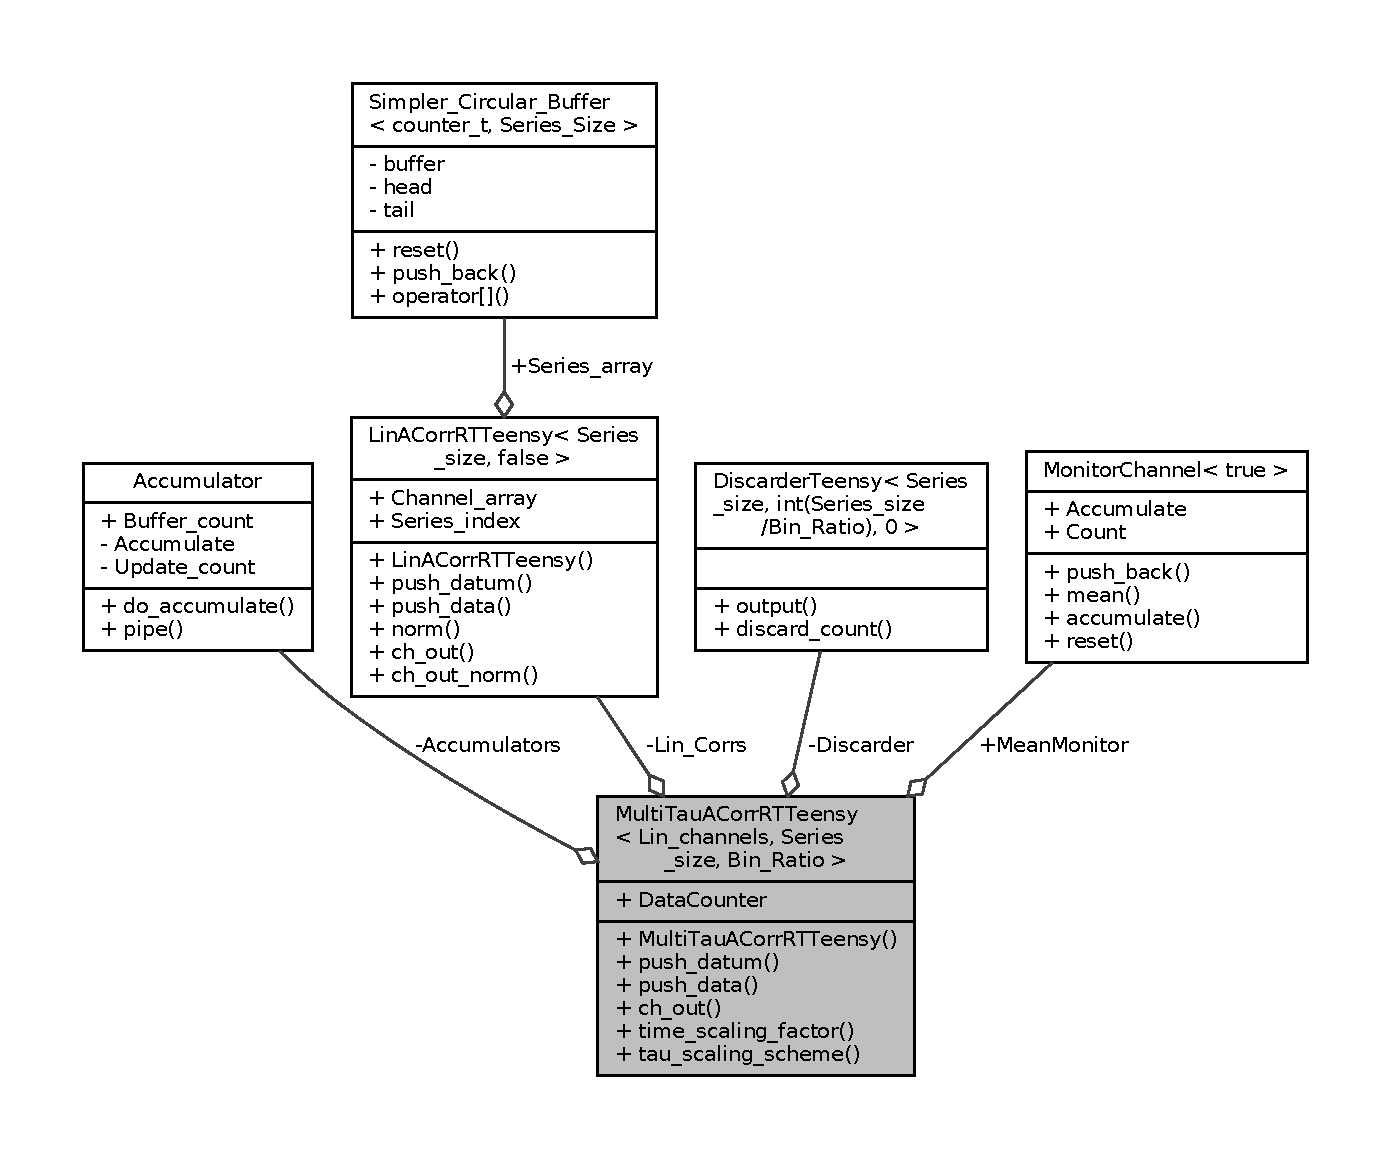
\includegraphics[width=350pt]{d8/d4e/classMultiTauACorrRTTeensy__coll__graph}
\end{center}
\end{figure}
\subsection*{Public Member Functions}
\begin{DoxyCompactItemize}
\item 
\hyperlink{classMultiTauACorrRTTeensy_a46b73c98f07f536603a8f5b2b3174d91}{Multi\+Tau\+A\+Corr\+R\+T\+Teensy} ()
\begin{DoxyCompactList}\small\item\em Counts the total number of data points sent to the counter. \end{DoxyCompactList}\item 
void \hyperlink{classMultiTauACorrRTTeensy_a85777a221b7a15de34b252ed804ab0f8}{push\+\_\+datum} (\hyperlink{types_8hpp_a22f279793847eba127de149437848c48}{counter\+\_\+t} datum) \+\_\+\+\_\+attribute\+\_\+\+\_\+((flatten))
\begin{DoxyCompactList}\small\item\em Pushes the datum to each of the Linear Correlators through the \hyperlink{classAccumulator}{Accumulator} adapter. \end{DoxyCompactList}\item 
void \hyperlink{classMultiTauACorrRTTeensy_ad3c078b834bb1682c93ba4cd5639d450}{push\+\_\+data} (const \hyperlink{types_8hpp_a22f279793847eba127de149437848c48}{counter\+\_\+t} $\ast$container, const \hyperlink{types_8hpp_ab41b824af8e088d090c0b9e60f536c9d}{index\+\_\+t} size) \+\_\+\+\_\+attribute\+\_\+\+\_\+((flatten))
\begin{DoxyCompactList}\small\item\em Repeatedly calls the Multi\+Tau\+\_\+\+A\+Corr\+\_\+\+R\+T\+::push\+\_\+datum() on the given container of counter values. \end{DoxyCompactList}\item 
void \hyperlink{classMultiTauACorrRTTeensy_af9ab6f055c1efc4a28c7c5bfa3aea074}{ch\+\_\+out} () const \+\_\+\+\_\+attribute\+\_\+\+\_\+((flatten))
\begin{DoxyCompactList}\small\item\em Outputs the Linear Correlator channels through the discarder adapter. \end{DoxyCompactList}\item 
\hyperlink{types_8hpp_ab41b824af8e088d090c0b9e60f536c9d}{index\+\_\+t} \hyperlink{classMultiTauACorrRTTeensy_a56fbc9bf757ac74e0dad862ec45def82}{time\+\_\+scaling\+\_\+factor} () const \+\_\+\+\_\+attribute\+\_\+\+\_\+((always\+\_\+inline))
\item 
\hyperlink{types_8hpp_ab41b824af8e088d090c0b9e60f536c9d}{index\+\_\+t} \hyperlink{classMultiTauACorrRTTeensy_a1a677c901b40aecdd00a4f2135d8c2bb}{tau\+\_\+scaling\+\_\+scheme} (unsigned int s) const \+\_\+\+\_\+attribute\+\_\+\+\_\+((always\+\_\+inline))
\begin{DoxyCompactList}\small\item\em Returns the relavent Tau scaling factor, based on the specialised scheme. It is used by the accumulator objects to set the Buffer\+Points attribute. \end{DoxyCompactList}\end{DoxyCompactItemize}
\subsection*{Public Attributes}
\begin{DoxyCompactItemize}
\item 
\hyperlink{classMonitorChannel}{Monitor\+Channel}$<$ true $>$ \hyperlink{classMultiTauACorrRTTeensy_a88f0486f59451fb97a787741c80badf9}{Mean\+Monitor}
\item 
uint32\+\_\+t \hyperlink{classMultiTauACorrRTTeensy_ab2fa5a0800fa7d9ee52900ced06ce935}{Data\+Counter} = 0
\end{DoxyCompactItemize}
\subsection*{Private Attributes}
\begin{DoxyCompactItemize}
\item 
\hyperlink{classAccumulator}{Accumulator} \hyperlink{classMultiTauACorrRTTeensy_aac3d87dfb6b995e83e20f444d3d5eb0d}{Accumulators} \mbox{[}Lin\+\_\+channels\mbox{]}
\begin{DoxyCompactList}\small\item\em \hyperlink{classAccumulator}{Accumulator} Objects for each channel (\hyperlink{classAccumulator}{Accumulator} \textquotesingle{}0\textquotesingle{} is redundant.) \end{DoxyCompactList}\item 
\hyperlink{classLinACorrRTTeensy}{Lin\+A\+Corr\+R\+T\+Teensy}$<$ Series\+\_\+size, false $>$ \hyperlink{classMultiTauACorrRTTeensy_abd0498010dea716140e242ccbf426174}{Lin\+\_\+\+Corrs} \mbox{[}Lin\+\_\+channels\mbox{]}
\begin{DoxyCompactList}\small\item\em Linear A\+Correlators. \end{DoxyCompactList}\item 
\hyperlink{classDiscarderTeensy}{Discarder\+Teensy}$<$ Series\+\_\+size, int(Series\+\_\+size/Bin\+\_\+\+Ratio), 0 $>$ \hyperlink{classMultiTauACorrRTTeensy_ad7bd7663180cdc3702ada3e726486311}{Discarder}
\begin{DoxyCompactList}\small\item\em Discarder that discards first \#\+Bin\+\_\+\+Ratio points. \end{DoxyCompactList}\end{DoxyCompactItemize}


\subsection{Detailed Description}
\subsubsection*{template$<$unsigned int Lin\+\_\+channels, index\+\_\+t Series\+\_\+size, unsigned int Bin\+\_\+\+Ratio$>$\newline
class Multi\+Tau\+A\+Corr\+R\+T\+Teensy$<$ Lin\+\_\+channels, Series\+\_\+size, Bin\+\_\+\+Ratio $>$}

Multi\+Tau Auto-\/\+Correlator object that is composed of multiple linear -\/ autocorrelators. Specialised for teensy. 

\subsection{Constructor \& Destructor Documentation}
\mbox{\Hypertarget{classMultiTauACorrRTTeensy_a46b73c98f07f536603a8f5b2b3174d91}\label{classMultiTauACorrRTTeensy_a46b73c98f07f536603a8f5b2b3174d91}} 
\index{Multi\+Tau\+A\+Corr\+R\+T\+Teensy@{Multi\+Tau\+A\+Corr\+R\+T\+Teensy}!Multi\+Tau\+A\+Corr\+R\+T\+Teensy@{Multi\+Tau\+A\+Corr\+R\+T\+Teensy}}
\index{Multi\+Tau\+A\+Corr\+R\+T\+Teensy@{Multi\+Tau\+A\+Corr\+R\+T\+Teensy}!Multi\+Tau\+A\+Corr\+R\+T\+Teensy@{Multi\+Tau\+A\+Corr\+R\+T\+Teensy}}
\subsubsection{\texorpdfstring{Multi\+Tau\+A\+Corr\+R\+T\+Teensy()}{MultiTauACorrRTTeensy()}}
{\footnotesize\ttfamily template$<$unsigned int Lin\+\_\+channels, index\+\_\+t Series\+\_\+size, unsigned int Bin\+\_\+\+Ratio$>$ \\
\hyperlink{classMultiTauACorrRTTeensy}{Multi\+Tau\+A\+Corr\+R\+T\+Teensy}$<$ Lin\+\_\+channels, Series\+\_\+size, Bin\+\_\+\+Ratio $>$\+::\hyperlink{classMultiTauACorrRTTeensy}{Multi\+Tau\+A\+Corr\+R\+T\+Teensy} (\begin{DoxyParamCaption}{ }\end{DoxyParamCaption})\hspace{0.3cm}{\ttfamily [inline]}}



Counts the total number of data points sent to the counter. 

Default Contructor -\/ Initalizes the Buffer\+Points attribute in the correlators. 

\subsection{Member Function Documentation}
\mbox{\Hypertarget{classMultiTauACorrRTTeensy_af9ab6f055c1efc4a28c7c5bfa3aea074}\label{classMultiTauACorrRTTeensy_af9ab6f055c1efc4a28c7c5bfa3aea074}} 
\index{Multi\+Tau\+A\+Corr\+R\+T\+Teensy@{Multi\+Tau\+A\+Corr\+R\+T\+Teensy}!ch\+\_\+out@{ch\+\_\+out}}
\index{ch\+\_\+out@{ch\+\_\+out}!Multi\+Tau\+A\+Corr\+R\+T\+Teensy@{Multi\+Tau\+A\+Corr\+R\+T\+Teensy}}
\subsubsection{\texorpdfstring{ch\+\_\+out()}{ch\_out()}}
{\footnotesize\ttfamily template$<$unsigned int Lin\+\_\+channels, index\+\_\+t Series\+\_\+size, unsigned int Bin\+\_\+\+Ratio$>$ \\
void \hyperlink{classMultiTauACorrRTTeensy}{Multi\+Tau\+A\+Corr\+R\+T\+Teensy}$<$ Lin\+\_\+channels, Series\+\_\+size, Bin\+\_\+\+Ratio $>$\+::ch\+\_\+out (\begin{DoxyParamCaption}{ }\end{DoxyParamCaption}) const\hspace{0.3cm}{\ttfamily [inline]}}



Outputs the Linear Correlator channels through the discarder adapter. 

\mbox{\Hypertarget{classMultiTauACorrRTTeensy_ad3c078b834bb1682c93ba4cd5639d450}\label{classMultiTauACorrRTTeensy_ad3c078b834bb1682c93ba4cd5639d450}} 
\index{Multi\+Tau\+A\+Corr\+R\+T\+Teensy@{Multi\+Tau\+A\+Corr\+R\+T\+Teensy}!push\+\_\+data@{push\+\_\+data}}
\index{push\+\_\+data@{push\+\_\+data}!Multi\+Tau\+A\+Corr\+R\+T\+Teensy@{Multi\+Tau\+A\+Corr\+R\+T\+Teensy}}
\subsubsection{\texorpdfstring{push\+\_\+data()}{push\_data()}}
{\footnotesize\ttfamily template$<$unsigned int Lin\+\_\+channels, index\+\_\+t Series\+\_\+size, unsigned int Bin\+\_\+\+Ratio$>$ \\
void \hyperlink{classMultiTauACorrRTTeensy}{Multi\+Tau\+A\+Corr\+R\+T\+Teensy}$<$ Lin\+\_\+channels, Series\+\_\+size, Bin\+\_\+\+Ratio $>$\+::push\+\_\+data (\begin{DoxyParamCaption}\item[{const \hyperlink{types_8hpp_a22f279793847eba127de149437848c48}{counter\+\_\+t} $\ast$}]{container,  }\item[{const \hyperlink{types_8hpp_ab41b824af8e088d090c0b9e60f536c9d}{index\+\_\+t}}]{size }\end{DoxyParamCaption})\hspace{0.3cm}{\ttfamily [inline]}}



Repeatedly calls the Multi\+Tau\+\_\+\+A\+Corr\+\_\+\+R\+T\+::push\+\_\+datum() on the given container of counter values. 

\mbox{\Hypertarget{classMultiTauACorrRTTeensy_a85777a221b7a15de34b252ed804ab0f8}\label{classMultiTauACorrRTTeensy_a85777a221b7a15de34b252ed804ab0f8}} 
\index{Multi\+Tau\+A\+Corr\+R\+T\+Teensy@{Multi\+Tau\+A\+Corr\+R\+T\+Teensy}!push\+\_\+datum@{push\+\_\+datum}}
\index{push\+\_\+datum@{push\+\_\+datum}!Multi\+Tau\+A\+Corr\+R\+T\+Teensy@{Multi\+Tau\+A\+Corr\+R\+T\+Teensy}}
\subsubsection{\texorpdfstring{push\+\_\+datum()}{push\_datum()}}
{\footnotesize\ttfamily template$<$unsigned int Lin\+\_\+channels, index\+\_\+t Series\+\_\+size, unsigned int Bin\+\_\+\+Ratio$>$ \\
void \hyperlink{classMultiTauACorrRTTeensy}{Multi\+Tau\+A\+Corr\+R\+T\+Teensy}$<$ Lin\+\_\+channels, Series\+\_\+size, Bin\+\_\+\+Ratio $>$\+::push\+\_\+datum (\begin{DoxyParamCaption}\item[{\hyperlink{types_8hpp_a22f279793847eba127de149437848c48}{counter\+\_\+t}}]{datum }\end{DoxyParamCaption})\hspace{0.3cm}{\ttfamily [inline]}}



Pushes the datum to each of the Linear Correlators through the \hyperlink{classAccumulator}{Accumulator} adapter. 

\mbox{\Hypertarget{classMultiTauACorrRTTeensy_a1a677c901b40aecdd00a4f2135d8c2bb}\label{classMultiTauACorrRTTeensy_a1a677c901b40aecdd00a4f2135d8c2bb}} 
\index{Multi\+Tau\+A\+Corr\+R\+T\+Teensy@{Multi\+Tau\+A\+Corr\+R\+T\+Teensy}!tau\+\_\+scaling\+\_\+scheme@{tau\+\_\+scaling\+\_\+scheme}}
\index{tau\+\_\+scaling\+\_\+scheme@{tau\+\_\+scaling\+\_\+scheme}!Multi\+Tau\+A\+Corr\+R\+T\+Teensy@{Multi\+Tau\+A\+Corr\+R\+T\+Teensy}}
\subsubsection{\texorpdfstring{tau\+\_\+scaling\+\_\+scheme()}{tau\_scaling\_scheme()}}
{\footnotesize\ttfamily template$<$unsigned int Lin\+\_\+channels, index\+\_\+t Series\+\_\+size, unsigned int Bin\+\_\+\+Ratio$>$ \\
\hyperlink{types_8hpp_ab41b824af8e088d090c0b9e60f536c9d}{index\+\_\+t} \hyperlink{classMultiTauACorrRTTeensy}{Multi\+Tau\+A\+Corr\+R\+T\+Teensy}$<$ Lin\+\_\+channels, Series\+\_\+size, Bin\+\_\+\+Ratio $>$\+::tau\+\_\+scaling\+\_\+scheme (\begin{DoxyParamCaption}\item[{unsigned int}]{s }\end{DoxyParamCaption}) const\hspace{0.3cm}{\ttfamily [inline]}}



Returns the relavent Tau scaling factor, based on the specialised scheme. It is used by the accumulator objects to set the Buffer\+Points attribute. 

\mbox{\Hypertarget{classMultiTauACorrRTTeensy_a56fbc9bf757ac74e0dad862ec45def82}\label{classMultiTauACorrRTTeensy_a56fbc9bf757ac74e0dad862ec45def82}} 
\index{Multi\+Tau\+A\+Corr\+R\+T\+Teensy@{Multi\+Tau\+A\+Corr\+R\+T\+Teensy}!time\+\_\+scaling\+\_\+factor@{time\+\_\+scaling\+\_\+factor}}
\index{time\+\_\+scaling\+\_\+factor@{time\+\_\+scaling\+\_\+factor}!Multi\+Tau\+A\+Corr\+R\+T\+Teensy@{Multi\+Tau\+A\+Corr\+R\+T\+Teensy}}
\subsubsection{\texorpdfstring{time\+\_\+scaling\+\_\+factor()}{time\_scaling\_factor()}}
{\footnotesize\ttfamily template$<$unsigned int Lin\+\_\+channels, index\+\_\+t Series\+\_\+size, unsigned int Bin\+\_\+\+Ratio$>$ \\
\hyperlink{types_8hpp_ab41b824af8e088d090c0b9e60f536c9d}{index\+\_\+t} \hyperlink{classMultiTauACorrRTTeensy}{Multi\+Tau\+A\+Corr\+R\+T\+Teensy}$<$ Lin\+\_\+channels, Series\+\_\+size, Bin\+\_\+\+Ratio $>$\+::time\+\_\+scaling\+\_\+factor (\begin{DoxyParamCaption}{ }\end{DoxyParamCaption}) const\hspace{0.3cm}{\ttfamily [inline]}}

Returns the number of data points after which, the timescale is scaled according to the Multi\+Tau\+\_\+\+A\+Corr\+\_\+\+R\+T\+::tau\+\_\+scaling\+\_\+scheme(). 

\subsection{Member Data Documentation}
\mbox{\Hypertarget{classMultiTauACorrRTTeensy_aac3d87dfb6b995e83e20f444d3d5eb0d}\label{classMultiTauACorrRTTeensy_aac3d87dfb6b995e83e20f444d3d5eb0d}} 
\index{Multi\+Tau\+A\+Corr\+R\+T\+Teensy@{Multi\+Tau\+A\+Corr\+R\+T\+Teensy}!Accumulators@{Accumulators}}
\index{Accumulators@{Accumulators}!Multi\+Tau\+A\+Corr\+R\+T\+Teensy@{Multi\+Tau\+A\+Corr\+R\+T\+Teensy}}
\subsubsection{\texorpdfstring{Accumulators}{Accumulators}}
{\footnotesize\ttfamily template$<$unsigned int Lin\+\_\+channels, index\+\_\+t Series\+\_\+size, unsigned int Bin\+\_\+\+Ratio$>$ \\
\hyperlink{classAccumulator}{Accumulator} \hyperlink{classMultiTauACorrRTTeensy}{Multi\+Tau\+A\+Corr\+R\+T\+Teensy}$<$ Lin\+\_\+channels, Series\+\_\+size, Bin\+\_\+\+Ratio $>$\+::Accumulators\mbox{[}Lin\+\_\+channels\mbox{]}\hspace{0.3cm}{\ttfamily [private]}}



\hyperlink{classAccumulator}{Accumulator} Objects for each channel (\hyperlink{classAccumulator}{Accumulator} \textquotesingle{}0\textquotesingle{} is redundant.) 

\mbox{\Hypertarget{classMultiTauACorrRTTeensy_ab2fa5a0800fa7d9ee52900ced06ce935}\label{classMultiTauACorrRTTeensy_ab2fa5a0800fa7d9ee52900ced06ce935}} 
\index{Multi\+Tau\+A\+Corr\+R\+T\+Teensy@{Multi\+Tau\+A\+Corr\+R\+T\+Teensy}!Data\+Counter@{Data\+Counter}}
\index{Data\+Counter@{Data\+Counter}!Multi\+Tau\+A\+Corr\+R\+T\+Teensy@{Multi\+Tau\+A\+Corr\+R\+T\+Teensy}}
\subsubsection{\texorpdfstring{Data\+Counter}{DataCounter}}
{\footnotesize\ttfamily template$<$unsigned int Lin\+\_\+channels, index\+\_\+t Series\+\_\+size, unsigned int Bin\+\_\+\+Ratio$>$ \\
uint32\+\_\+t \hyperlink{classMultiTauACorrRTTeensy}{Multi\+Tau\+A\+Corr\+R\+T\+Teensy}$<$ Lin\+\_\+channels, Series\+\_\+size, Bin\+\_\+\+Ratio $>$\+::Data\+Counter = 0}

\mbox{\Hypertarget{classMultiTauACorrRTTeensy_ad7bd7663180cdc3702ada3e726486311}\label{classMultiTauACorrRTTeensy_ad7bd7663180cdc3702ada3e726486311}} 
\index{Multi\+Tau\+A\+Corr\+R\+T\+Teensy@{Multi\+Tau\+A\+Corr\+R\+T\+Teensy}!Discarder@{Discarder}}
\index{Discarder@{Discarder}!Multi\+Tau\+A\+Corr\+R\+T\+Teensy@{Multi\+Tau\+A\+Corr\+R\+T\+Teensy}}
\subsubsection{\texorpdfstring{Discarder}{Discarder}}
{\footnotesize\ttfamily template$<$unsigned int Lin\+\_\+channels, index\+\_\+t Series\+\_\+size, unsigned int Bin\+\_\+\+Ratio$>$ \\
\hyperlink{classDiscarderTeensy}{Discarder\+Teensy}$<$Series\+\_\+size, int(Series\+\_\+size/Bin\+\_\+\+Ratio), 0$>$ \hyperlink{classMultiTauACorrRTTeensy}{Multi\+Tau\+A\+Corr\+R\+T\+Teensy}$<$ Lin\+\_\+channels, Series\+\_\+size, Bin\+\_\+\+Ratio $>$\+::Discarder\hspace{0.3cm}{\ttfamily [private]}}



Discarder that discards first \#\+Bin\+\_\+\+Ratio points. 

\mbox{\Hypertarget{classMultiTauACorrRTTeensy_abd0498010dea716140e242ccbf426174}\label{classMultiTauACorrRTTeensy_abd0498010dea716140e242ccbf426174}} 
\index{Multi\+Tau\+A\+Corr\+R\+T\+Teensy@{Multi\+Tau\+A\+Corr\+R\+T\+Teensy}!Lin\+\_\+\+Corrs@{Lin\+\_\+\+Corrs}}
\index{Lin\+\_\+\+Corrs@{Lin\+\_\+\+Corrs}!Multi\+Tau\+A\+Corr\+R\+T\+Teensy@{Multi\+Tau\+A\+Corr\+R\+T\+Teensy}}
\subsubsection{\texorpdfstring{Lin\+\_\+\+Corrs}{Lin\_Corrs}}
{\footnotesize\ttfamily template$<$unsigned int Lin\+\_\+channels, index\+\_\+t Series\+\_\+size, unsigned int Bin\+\_\+\+Ratio$>$ \\
\hyperlink{classLinACorrRTTeensy}{Lin\+A\+Corr\+R\+T\+Teensy}$<$Series\+\_\+size, false$>$ \hyperlink{classMultiTauACorrRTTeensy}{Multi\+Tau\+A\+Corr\+R\+T\+Teensy}$<$ Lin\+\_\+channels, Series\+\_\+size, Bin\+\_\+\+Ratio $>$\+::Lin\+\_\+\+Corrs\mbox{[}Lin\+\_\+channels\mbox{]}\hspace{0.3cm}{\ttfamily [private]}}



Linear A\+Correlators. 

\mbox{\Hypertarget{classMultiTauACorrRTTeensy_a88f0486f59451fb97a787741c80badf9}\label{classMultiTauACorrRTTeensy_a88f0486f59451fb97a787741c80badf9}} 
\index{Multi\+Tau\+A\+Corr\+R\+T\+Teensy@{Multi\+Tau\+A\+Corr\+R\+T\+Teensy}!Mean\+Monitor@{Mean\+Monitor}}
\index{Mean\+Monitor@{Mean\+Monitor}!Multi\+Tau\+A\+Corr\+R\+T\+Teensy@{Multi\+Tau\+A\+Corr\+R\+T\+Teensy}}
\subsubsection{\texorpdfstring{Mean\+Monitor}{MeanMonitor}}
{\footnotesize\ttfamily template$<$unsigned int Lin\+\_\+channels, index\+\_\+t Series\+\_\+size, unsigned int Bin\+\_\+\+Ratio$>$ \\
\hyperlink{classMonitorChannel}{Monitor\+Channel}$<$true$>$ \hyperlink{classMultiTauACorrRTTeensy}{Multi\+Tau\+A\+Corr\+R\+T\+Teensy}$<$ Lin\+\_\+channels, Series\+\_\+size, Bin\+\_\+\+Ratio $>$\+::Mean\+Monitor}



The documentation for this class was generated from the following file\+:\begin{DoxyCompactItemize}
\item 
code/software/\hyperlink{multi__tau_8hpp}{multi\+\_\+tau.\+hpp}\end{DoxyCompactItemize}

\hypertarget{classnormalizer_1_1Normalizer}{}\section{normalizer.\+Normalizer Class Reference}
\label{classnormalizer_1_1Normalizer}\index{normalizer.\+Normalizer@{normalizer.\+Normalizer}}
\subsection*{Public Member Functions}
\begin{DoxyCompactItemize}
\item 
def \hyperlink{classnormalizer_1_1Normalizer_afccec17549a3a8de54c39b7b5de3d4b7}{\+\_\+\+\_\+init\+\_\+\+\_\+} (self, lin\+\_\+corrs, series\+\_\+size, bin\+\_\+ratio)
\item 
def \hyperlink{classnormalizer_1_1Normalizer_ab4e48dd4987836c7254f148672dc32f0}{set\+\_\+mode} (self, mode\+\_\+str)
\item 
def \hyperlink{classnormalizer_1_1Normalizer_acae7ff724a12ef29c97f6eb2d30f5d62}{normalize} (self, input\+\_\+y, args)
\item 
def \hyperlink{classnormalizer_1_1Normalizer_a7965c29d7d3a867dbb82cc7f3e7e69b3}{no\+\_\+norm} (self, input\+\_\+y)
\item 
def \hyperlink{classnormalizer_1_1Normalizer_a44aea90aa5ab90fbc6cc617acdc589c5}{points\+\_\+norm} (self, input\+\_\+y, points\+\_\+no)
\item 
def \hyperlink{classnormalizer_1_1Normalizer_ac9530ba0efaa543756ecfef0e871b63e}{mean\+\_\+norm} (self, input\+\_\+y, points\+\_\+no, accumulate)
\item 
def \hyperlink{classnormalizer_1_1Normalizer_a09b6d62bec3fca383a1a9c82cc74836a}{\+\_\+\+\_\+repr\+\_\+\+\_\+} (self)
\end{DoxyCompactItemize}
\subsection*{Public Attributes}
\begin{DoxyCompactItemize}
\item 
\hyperlink{classnormalizer_1_1Normalizer_a63904e0449ec33d948edb1e00eda6bec}{mt\+\_\+param}
\item 
\hyperlink{classnormalizer_1_1Normalizer_adbbbab69e55b4a0593122aa61e7853bc}{points\+\_\+scale\+\_\+template}
\item 
\hyperlink{classnormalizer_1_1Normalizer_a0d063c22fb9e3ee66192bbeb570c2c3e}{bin\+\_\+ratio\+\_\+scale}
\item 
\hyperlink{classnormalizer_1_1Normalizer_a0db45b11e7934a2ce3cdbabc54467164}{bin\+\_\+ratio\+\_\+scale\+\_\+sq}
\item 
\hyperlink{classnormalizer_1_1Normalizer_ae6fdb25c519b72b0f95cc4b2ce150f45}{tau\+\_\+values}
\item 
\hyperlink{classnormalizer_1_1Normalizer_a0fe7ba5c6b5ba3df8578d7edf8bd3ade}{available\+\_\+modes}
\item 
\hyperlink{classnormalizer_1_1Normalizer_a36df68fe4c6f2dbe72f08a71ad1c5fe1}{norm\+\_\+fn}
\end{DoxyCompactItemize}


\subsection{Constructor \& Destructor Documentation}
\mbox{\Hypertarget{classnormalizer_1_1Normalizer_afccec17549a3a8de54c39b7b5de3d4b7}\label{classnormalizer_1_1Normalizer_afccec17549a3a8de54c39b7b5de3d4b7}} 
\index{normalizer\+::\+Normalizer@{normalizer\+::\+Normalizer}!\+\_\+\+\_\+init\+\_\+\+\_\+@{\+\_\+\+\_\+init\+\_\+\+\_\+}}
\index{\+\_\+\+\_\+init\+\_\+\+\_\+@{\+\_\+\+\_\+init\+\_\+\+\_\+}!normalizer\+::\+Normalizer@{normalizer\+::\+Normalizer}}
\subsubsection{\texorpdfstring{\+\_\+\+\_\+init\+\_\+\+\_\+()}{\_\_init\_\_()}}
{\footnotesize\ttfamily def normalizer.\+Normalizer.\+\_\+\+\_\+init\+\_\+\+\_\+ (\begin{DoxyParamCaption}\item[{}]{self,  }\item[{}]{lin\+\_\+corrs,  }\item[{}]{series\+\_\+size,  }\item[{}]{bin\+\_\+ratio }\end{DoxyParamCaption})}

\begin{DoxyVerb}Constructor that accepts multi-tau configuration parameters.
\end{DoxyVerb}
 

\subsection{Member Function Documentation}
\mbox{\Hypertarget{classnormalizer_1_1Normalizer_a09b6d62bec3fca383a1a9c82cc74836a}\label{classnormalizer_1_1Normalizer_a09b6d62bec3fca383a1a9c82cc74836a}} 
\index{normalizer\+::\+Normalizer@{normalizer\+::\+Normalizer}!\+\_\+\+\_\+repr\+\_\+\+\_\+@{\+\_\+\+\_\+repr\+\_\+\+\_\+}}
\index{\+\_\+\+\_\+repr\+\_\+\+\_\+@{\+\_\+\+\_\+repr\+\_\+\+\_\+}!normalizer\+::\+Normalizer@{normalizer\+::\+Normalizer}}
\subsubsection{\texorpdfstring{\+\_\+\+\_\+repr\+\_\+\+\_\+()}{\_\_repr\_\_()}}
{\footnotesize\ttfamily def normalizer.\+Normalizer.\+\_\+\+\_\+repr\+\_\+\+\_\+ (\begin{DoxyParamCaption}\item[{}]{self }\end{DoxyParamCaption})}

\mbox{\Hypertarget{classnormalizer_1_1Normalizer_ac9530ba0efaa543756ecfef0e871b63e}\label{classnormalizer_1_1Normalizer_ac9530ba0efaa543756ecfef0e871b63e}} 
\index{normalizer\+::\+Normalizer@{normalizer\+::\+Normalizer}!mean\+\_\+norm@{mean\+\_\+norm}}
\index{mean\+\_\+norm@{mean\+\_\+norm}!normalizer\+::\+Normalizer@{normalizer\+::\+Normalizer}}
\subsubsection{\texorpdfstring{mean\+\_\+norm()}{mean\_norm()}}
{\footnotesize\ttfamily def normalizer.\+Normalizer.\+mean\+\_\+norm (\begin{DoxyParamCaption}\item[{}]{self,  }\item[{}]{input\+\_\+y,  }\item[{}]{points\+\_\+no,  }\item[{}]{accumulate }\end{DoxyParamCaption})}

\begin{DoxyVerb}Returns the mean normalized transformation of the input. Accepts the number of points received by each 
channel and the mean monitor accumulate. Mean = accumulate / points_no.
\end{DoxyVerb}
 \mbox{\Hypertarget{classnormalizer_1_1Normalizer_a7965c29d7d3a867dbb82cc7f3e7e69b3}\label{classnormalizer_1_1Normalizer_a7965c29d7d3a867dbb82cc7f3e7e69b3}} 
\index{normalizer\+::\+Normalizer@{normalizer\+::\+Normalizer}!no\+\_\+norm@{no\+\_\+norm}}
\index{no\+\_\+norm@{no\+\_\+norm}!normalizer\+::\+Normalizer@{normalizer\+::\+Normalizer}}
\subsubsection{\texorpdfstring{no\+\_\+norm()}{no\_norm()}}
{\footnotesize\ttfamily def normalizer.\+Normalizer.\+no\+\_\+norm (\begin{DoxyParamCaption}\item[{}]{self,  }\item[{}]{input\+\_\+y }\end{DoxyParamCaption})}

\begin{DoxyVerb}Returns a non-normalized sequence. This function does nothing except return its input.
\end{DoxyVerb}
 \mbox{\Hypertarget{classnormalizer_1_1Normalizer_acae7ff724a12ef29c97f6eb2d30f5d62}\label{classnormalizer_1_1Normalizer_acae7ff724a12ef29c97f6eb2d30f5d62}} 
\index{normalizer\+::\+Normalizer@{normalizer\+::\+Normalizer}!normalize@{normalize}}
\index{normalize@{normalize}!normalizer\+::\+Normalizer@{normalizer\+::\+Normalizer}}
\subsubsection{\texorpdfstring{normalize()}{normalize()}}
{\footnotesize\ttfamily def normalizer.\+Normalizer.\+normalize (\begin{DoxyParamCaption}\item[{}]{self,  }\item[{}]{input\+\_\+y,  }\item[{}]{args }\end{DoxyParamCaption})}

\begin{DoxyVerb}Callable normalization function - single interface.
\end{DoxyVerb}
 \mbox{\Hypertarget{classnormalizer_1_1Normalizer_a44aea90aa5ab90fbc6cc617acdc589c5}\label{classnormalizer_1_1Normalizer_a44aea90aa5ab90fbc6cc617acdc589c5}} 
\index{normalizer\+::\+Normalizer@{normalizer\+::\+Normalizer}!points\+\_\+norm@{points\+\_\+norm}}
\index{points\+\_\+norm@{points\+\_\+norm}!normalizer\+::\+Normalizer@{normalizer\+::\+Normalizer}}
\subsubsection{\texorpdfstring{points\+\_\+norm()}{points\_norm()}}
{\footnotesize\ttfamily def normalizer.\+Normalizer.\+points\+\_\+norm (\begin{DoxyParamCaption}\item[{}]{self,  }\item[{}]{input\+\_\+y,  }\item[{}]{points\+\_\+no }\end{DoxyParamCaption})}

\begin{DoxyVerb}Returns the input by dividing it with the number of points received by that particular channel.
\end{DoxyVerb}
 \mbox{\Hypertarget{classnormalizer_1_1Normalizer_ab4e48dd4987836c7254f148672dc32f0}\label{classnormalizer_1_1Normalizer_ab4e48dd4987836c7254f148672dc32f0}} 
\index{normalizer\+::\+Normalizer@{normalizer\+::\+Normalizer}!set\+\_\+mode@{set\+\_\+mode}}
\index{set\+\_\+mode@{set\+\_\+mode}!normalizer\+::\+Normalizer@{normalizer\+::\+Normalizer}}
\subsubsection{\texorpdfstring{set\+\_\+mode()}{set\_mode()}}
{\footnotesize\ttfamily def normalizer.\+Normalizer.\+set\+\_\+mode (\begin{DoxyParamCaption}\item[{}]{self,  }\item[{}]{mode\+\_\+str }\end{DoxyParamCaption})}

\begin{DoxyVerb}Sets the normalization mode for the normalizer. Accepted modes -> {"no", "points", "mean"}
\end{DoxyVerb}
 

\subsection{Member Data Documentation}
\mbox{\Hypertarget{classnormalizer_1_1Normalizer_a0fe7ba5c6b5ba3df8578d7edf8bd3ade}\label{classnormalizer_1_1Normalizer_a0fe7ba5c6b5ba3df8578d7edf8bd3ade}} 
\index{normalizer\+::\+Normalizer@{normalizer\+::\+Normalizer}!available\+\_\+modes@{available\+\_\+modes}}
\index{available\+\_\+modes@{available\+\_\+modes}!normalizer\+::\+Normalizer@{normalizer\+::\+Normalizer}}
\subsubsection{\texorpdfstring{available\+\_\+modes}{available\_modes}}
{\footnotesize\ttfamily normalizer.\+Normalizer.\+available\+\_\+modes}

\mbox{\Hypertarget{classnormalizer_1_1Normalizer_a0d063c22fb9e3ee66192bbeb570c2c3e}\label{classnormalizer_1_1Normalizer_a0d063c22fb9e3ee66192bbeb570c2c3e}} 
\index{normalizer\+::\+Normalizer@{normalizer\+::\+Normalizer}!bin\+\_\+ratio\+\_\+scale@{bin\+\_\+ratio\+\_\+scale}}
\index{bin\+\_\+ratio\+\_\+scale@{bin\+\_\+ratio\+\_\+scale}!normalizer\+::\+Normalizer@{normalizer\+::\+Normalizer}}
\subsubsection{\texorpdfstring{bin\+\_\+ratio\+\_\+scale}{bin\_ratio\_scale}}
{\footnotesize\ttfamily normalizer.\+Normalizer.\+bin\+\_\+ratio\+\_\+scale}

\mbox{\Hypertarget{classnormalizer_1_1Normalizer_a0db45b11e7934a2ce3cdbabc54467164}\label{classnormalizer_1_1Normalizer_a0db45b11e7934a2ce3cdbabc54467164}} 
\index{normalizer\+::\+Normalizer@{normalizer\+::\+Normalizer}!bin\+\_\+ratio\+\_\+scale\+\_\+sq@{bin\+\_\+ratio\+\_\+scale\+\_\+sq}}
\index{bin\+\_\+ratio\+\_\+scale\+\_\+sq@{bin\+\_\+ratio\+\_\+scale\+\_\+sq}!normalizer\+::\+Normalizer@{normalizer\+::\+Normalizer}}
\subsubsection{\texorpdfstring{bin\+\_\+ratio\+\_\+scale\+\_\+sq}{bin\_ratio\_scale\_sq}}
{\footnotesize\ttfamily normalizer.\+Normalizer.\+bin\+\_\+ratio\+\_\+scale\+\_\+sq}

\mbox{\Hypertarget{classnormalizer_1_1Normalizer_a63904e0449ec33d948edb1e00eda6bec}\label{classnormalizer_1_1Normalizer_a63904e0449ec33d948edb1e00eda6bec}} 
\index{normalizer\+::\+Normalizer@{normalizer\+::\+Normalizer}!mt\+\_\+param@{mt\+\_\+param}}
\index{mt\+\_\+param@{mt\+\_\+param}!normalizer\+::\+Normalizer@{normalizer\+::\+Normalizer}}
\subsubsection{\texorpdfstring{mt\+\_\+param}{mt\_param}}
{\footnotesize\ttfamily normalizer.\+Normalizer.\+mt\+\_\+param}

\mbox{\Hypertarget{classnormalizer_1_1Normalizer_a36df68fe4c6f2dbe72f08a71ad1c5fe1}\label{classnormalizer_1_1Normalizer_a36df68fe4c6f2dbe72f08a71ad1c5fe1}} 
\index{normalizer\+::\+Normalizer@{normalizer\+::\+Normalizer}!norm\+\_\+fn@{norm\+\_\+fn}}
\index{norm\+\_\+fn@{norm\+\_\+fn}!normalizer\+::\+Normalizer@{normalizer\+::\+Normalizer}}
\subsubsection{\texorpdfstring{norm\+\_\+fn}{norm\_fn}}
{\footnotesize\ttfamily normalizer.\+Normalizer.\+norm\+\_\+fn}

\mbox{\Hypertarget{classnormalizer_1_1Normalizer_adbbbab69e55b4a0593122aa61e7853bc}\label{classnormalizer_1_1Normalizer_adbbbab69e55b4a0593122aa61e7853bc}} 
\index{normalizer\+::\+Normalizer@{normalizer\+::\+Normalizer}!points\+\_\+scale\+\_\+template@{points\+\_\+scale\+\_\+template}}
\index{points\+\_\+scale\+\_\+template@{points\+\_\+scale\+\_\+template}!normalizer\+::\+Normalizer@{normalizer\+::\+Normalizer}}
\subsubsection{\texorpdfstring{points\+\_\+scale\+\_\+template}{points\_scale\_template}}
{\footnotesize\ttfamily normalizer.\+Normalizer.\+points\+\_\+scale\+\_\+template}

\mbox{\Hypertarget{classnormalizer_1_1Normalizer_ae6fdb25c519b72b0f95cc4b2ce150f45}\label{classnormalizer_1_1Normalizer_ae6fdb25c519b72b0f95cc4b2ce150f45}} 
\index{normalizer\+::\+Normalizer@{normalizer\+::\+Normalizer}!tau\+\_\+values@{tau\+\_\+values}}
\index{tau\+\_\+values@{tau\+\_\+values}!normalizer\+::\+Normalizer@{normalizer\+::\+Normalizer}}
\subsubsection{\texorpdfstring{tau\+\_\+values}{tau\_values}}
{\footnotesize\ttfamily normalizer.\+Normalizer.\+tau\+\_\+values}



The documentation for this class was generated from the following file\+:\begin{DoxyCompactItemize}
\item 
code/pc\+\_\+app/\hyperlink{normalizer_8py}{normalizer.\+py}\end{DoxyCompactItemize}

\hypertarget{classutilities_1_1OffsetTracker}{}\section{utilities.\+Offset\+Tracker Class Reference}
\label{classutilities_1_1OffsetTracker}\index{utilities.\+Offset\+Tracker@{utilities.\+Offset\+Tracker}}
\subsection*{Public Member Functions}
\begin{DoxyCompactItemize}
\item 
def \hyperlink{classutilities_1_1OffsetTracker_a75d00b8c481ed3b39c2962b8e6e66b91}{\+\_\+\+\_\+init\+\_\+\+\_\+} (self)
\item 
def \hyperlink{classutilities_1_1OffsetTracker_a058ad5ae0b53bfbfecc4612e094951d5}{advance} (self, bytes\+\_\+read\+\_\+now=0)
\item 
def \hyperlink{classutilities_1_1OffsetTracker_a3ed692ec6058294066507626026b78f1}{offsetter} (self)
\end{DoxyCompactItemize}
\subsection*{Public Attributes}
\begin{DoxyCompactItemize}
\item 
\hyperlink{classutilities_1_1OffsetTracker_ac6ebf15df031eb10591c8e8a8d8e0168}{rd\+\_\+bytes}
\item 
\hyperlink{classutilities_1_1OffsetTracker_aa316b20e9e769ec032e38d902846f279}{gen}
\end{DoxyCompactItemize}


\subsection{Constructor \& Destructor Documentation}
\mbox{\Hypertarget{classutilities_1_1OffsetTracker_a75d00b8c481ed3b39c2962b8e6e66b91}\label{classutilities_1_1OffsetTracker_a75d00b8c481ed3b39c2962b8e6e66b91}} 
\index{utilities\+::\+Offset\+Tracker@{utilities\+::\+Offset\+Tracker}!\+\_\+\+\_\+init\+\_\+\+\_\+@{\+\_\+\+\_\+init\+\_\+\+\_\+}}
\index{\+\_\+\+\_\+init\+\_\+\+\_\+@{\+\_\+\+\_\+init\+\_\+\+\_\+}!utilities\+::\+Offset\+Tracker@{utilities\+::\+Offset\+Tracker}}
\subsubsection{\texorpdfstring{\+\_\+\+\_\+init\+\_\+\+\_\+()}{\_\_init\_\_()}}
{\footnotesize\ttfamily def utilities.\+Offset\+Tracker.\+\_\+\+\_\+init\+\_\+\+\_\+ (\begin{DoxyParamCaption}\item[{}]{self }\end{DoxyParamCaption})}



\subsection{Member Function Documentation}
\mbox{\Hypertarget{classutilities_1_1OffsetTracker_a058ad5ae0b53bfbfecc4612e094951d5}\label{classutilities_1_1OffsetTracker_a058ad5ae0b53bfbfecc4612e094951d5}} 
\index{utilities\+::\+Offset\+Tracker@{utilities\+::\+Offset\+Tracker}!advance@{advance}}
\index{advance@{advance}!utilities\+::\+Offset\+Tracker@{utilities\+::\+Offset\+Tracker}}
\subsubsection{\texorpdfstring{advance()}{advance()}}
{\footnotesize\ttfamily def utilities.\+Offset\+Tracker.\+advance (\begin{DoxyParamCaption}\item[{}]{self,  }\item[{}]{bytes\+\_\+read\+\_\+now = {\ttfamily 0} }\end{DoxyParamCaption})}

\begin{DoxyVerb}Returns the current offset value, while storing the 
`bytes_read_now` for generating the next offset.
\end{DoxyVerb}
 \mbox{\Hypertarget{classutilities_1_1OffsetTracker_a3ed692ec6058294066507626026b78f1}\label{classutilities_1_1OffsetTracker_a3ed692ec6058294066507626026b78f1}} 
\index{utilities\+::\+Offset\+Tracker@{utilities\+::\+Offset\+Tracker}!offsetter@{offsetter}}
\index{offsetter@{offsetter}!utilities\+::\+Offset\+Tracker@{utilities\+::\+Offset\+Tracker}}
\subsubsection{\texorpdfstring{offsetter()}{offsetter()}}
{\footnotesize\ttfamily def utilities.\+Offset\+Tracker.\+offsetter (\begin{DoxyParamCaption}\item[{}]{self }\end{DoxyParamCaption})}

\begin{DoxyVerb}Returns the current offset value.
\end{DoxyVerb}
 

\subsection{Member Data Documentation}
\mbox{\Hypertarget{classutilities_1_1OffsetTracker_aa316b20e9e769ec032e38d902846f279}\label{classutilities_1_1OffsetTracker_aa316b20e9e769ec032e38d902846f279}} 
\index{utilities\+::\+Offset\+Tracker@{utilities\+::\+Offset\+Tracker}!gen@{gen}}
\index{gen@{gen}!utilities\+::\+Offset\+Tracker@{utilities\+::\+Offset\+Tracker}}
\subsubsection{\texorpdfstring{gen}{gen}}
{\footnotesize\ttfamily utilities.\+Offset\+Tracker.\+gen}

\mbox{\Hypertarget{classutilities_1_1OffsetTracker_ac6ebf15df031eb10591c8e8a8d8e0168}\label{classutilities_1_1OffsetTracker_ac6ebf15df031eb10591c8e8a8d8e0168}} 
\index{utilities\+::\+Offset\+Tracker@{utilities\+::\+Offset\+Tracker}!rd\+\_\+bytes@{rd\+\_\+bytes}}
\index{rd\+\_\+bytes@{rd\+\_\+bytes}!utilities\+::\+Offset\+Tracker@{utilities\+::\+Offset\+Tracker}}
\subsubsection{\texorpdfstring{rd\+\_\+bytes}{rd\_bytes}}
{\footnotesize\ttfamily utilities.\+Offset\+Tracker.\+rd\+\_\+bytes}



The documentation for this class was generated from the following file\+:\begin{DoxyCompactItemize}
\item 
code/pc\+\_\+app/\hyperlink{utilities_8py}{utilities.\+py}\end{DoxyCompactItemize}

\hypertarget{classnew__app_1_1ParamStruct}{}\section{new\+\_\+app.\+Param\+Struct Class Reference}
\label{classnew__app_1_1ParamStruct}\index{new\+\_\+app.\+Param\+Struct@{new\+\_\+app.\+Param\+Struct}}
\subsection*{Public Member Functions}
\begin{DoxyCompactItemize}
\item 
def \hyperlink{classnew__app_1_1ParamStruct_aa1d6a92c83421312796c61a958fd92d0}{\+\_\+\+\_\+init\+\_\+\+\_\+} ()
\end{DoxyCompactItemize}


\subsection{Constructor \& Destructor Documentation}
\mbox{\Hypertarget{classnew__app_1_1ParamStruct_aa1d6a92c83421312796c61a958fd92d0}\label{classnew__app_1_1ParamStruct_aa1d6a92c83421312796c61a958fd92d0}} 
\index{new\+\_\+app\+::\+Param\+Struct@{new\+\_\+app\+::\+Param\+Struct}!\+\_\+\+\_\+init\+\_\+\+\_\+@{\+\_\+\+\_\+init\+\_\+\+\_\+}}
\index{\+\_\+\+\_\+init\+\_\+\+\_\+@{\+\_\+\+\_\+init\+\_\+\+\_\+}!new\+\_\+app\+::\+Param\+Struct@{new\+\_\+app\+::\+Param\+Struct}}
\subsubsection{\texorpdfstring{\+\_\+\+\_\+init\+\_\+\+\_\+()}{\_\_init\_\_()}}
{\footnotesize\ttfamily def new\+\_\+app.\+Param\+Struct.\+\_\+\+\_\+init\+\_\+\+\_\+ (\begin{DoxyParamCaption}{ }\end{DoxyParamCaption})}



The documentation for this class was generated from the following file\+:\begin{DoxyCompactItemize}
\item 
code/pc\+\_\+app/\hyperlink{new__app_8py}{new\+\_\+app.\+py}\end{DoxyCompactItemize}

\hypertarget{classPCHistogram}{}\section{P\+C\+Histogram$<$ Bin\+Type, Bins $>$ Class Template Reference}
\label{classPCHistogram}\index{P\+C\+Histogram$<$ Bin\+Type, Bins $>$@{P\+C\+Histogram$<$ Bin\+Type, Bins $>$}}


Photon Counting Histogram module for Real time calculation on {\itshape Teensy 4.\+1 microcontrollers}.  




{\ttfamily \#include $<$histogram.\+hpp$>$}

\subsection*{Public Member Functions}
\begin{DoxyCompactItemize}
\item 
constexpr unsigned int \hyperlink{classPCHistogram_a4c7558c7cebdd928c0b6e0c548baf1b9}{size} () \+\_\+\+\_\+attribute\+\_\+\+\_\+((always\+\_\+inline))
\begin{DoxyCompactList}\small\item\em Returns the total number of buns, including the overflow bin. \end{DoxyCompactList}\item 
{\footnotesize template$<$typename Data\+Type $>$ }\\void \hyperlink{classPCHistogram_a0885e66d0de46bd16b72b870d7f410fc}{push\+\_\+back} (Data\+Type datum)
\begin{DoxyCompactList}\small\item\em Receives a single datum and processes it to into the Histogram. \end{DoxyCompactList}\item 
void \hyperlink{classPCHistogram_af4391ac8ad3f4d9865ee6335fb563b4c}{output} () \+\_\+\+\_\+attribute\+\_\+\+\_\+((always\+\_\+inline))
\begin{DoxyCompactList}\small\item\em Sends the complete Histogram to the Serial output. \end{DoxyCompactList}\end{DoxyCompactItemize}
\subsection*{Public Attributes}
\begin{DoxyCompactItemize}
\item 
Bin\+Type \hyperlink{classPCHistogram_a239c7b1e34b2ecc1808e2304d71bc1e2}{Histogram} \mbox{[}Bins+1\mbox{]} = \{0\}
\begin{DoxyCompactList}\small\item\em Histogram function array. \end{DoxyCompactList}\end{DoxyCompactItemize}
\subsection*{Private Attributes}
\begin{DoxyCompactItemize}
\item 
unsigned int \hyperlink{classPCHistogram_a3d0371659763511d752c3348db978f79}{Index}
\begin{DoxyCompactList}\small\item\em Index used by the pushback function. \end{DoxyCompactList}\end{DoxyCompactItemize}


\subsection{Detailed Description}
\subsubsection*{template$<$typename Bin\+Type, unsigned int Bins$>$\newline
class P\+C\+Histogram$<$ Bin\+Type, Bins $>$}

Photon Counting Histogram module for Real time calculation on {\itshape Teensy 4.\+1 microcontrollers}. 

Describes a real time histogram function that is updated point by point. {\itshape The Bin index starts from zero.} The histogram\textquotesingle{}s lasrt bin, which is {\ttfamily Bins + 1}th bin is the overflow bin and includes all points above the maximum bin size. The histogram bin is left centred, i.\+e., the bin contains all numbers lower or equal to the Bin value. \begin{DoxyVerb}* [Bin 0][Bin 1][Bin 2][Bin 3][Bin 4]...[Bin Max][•|Bin Overflow|•]
* \end{DoxyVerb}
 

\subsection{Member Function Documentation}
\mbox{\Hypertarget{classPCHistogram_af4391ac8ad3f4d9865ee6335fb563b4c}\label{classPCHistogram_af4391ac8ad3f4d9865ee6335fb563b4c}} 
\index{P\+C\+Histogram@{P\+C\+Histogram}!output@{output}}
\index{output@{output}!P\+C\+Histogram@{P\+C\+Histogram}}
\subsubsection{\texorpdfstring{output()}{output()}}
{\footnotesize\ttfamily template$<$typename Bin\+Type, unsigned int Bins$>$ \\
void \hyperlink{classPCHistogram}{P\+C\+Histogram}$<$ Bin\+Type, Bins $>$\+::output (\begin{DoxyParamCaption}{ }\end{DoxyParamCaption})\hspace{0.3cm}{\ttfamily [inline]}}



Sends the complete Histogram to the Serial output. 

\mbox{\Hypertarget{classPCHistogram_a0885e66d0de46bd16b72b870d7f410fc}\label{classPCHistogram_a0885e66d0de46bd16b72b870d7f410fc}} 
\index{P\+C\+Histogram@{P\+C\+Histogram}!push\+\_\+back@{push\+\_\+back}}
\index{push\+\_\+back@{push\+\_\+back}!P\+C\+Histogram@{P\+C\+Histogram}}
\subsubsection{\texorpdfstring{push\+\_\+back()}{push\_back()}}
{\footnotesize\ttfamily template$<$typename Bin\+Type, unsigned int Bins$>$ \\
template$<$typename Data\+Type $>$ \\
void \hyperlink{classPCHistogram}{P\+C\+Histogram}$<$ Bin\+Type, Bins $>$\+::push\+\_\+back (\begin{DoxyParamCaption}\item[{Data\+Type}]{datum }\end{DoxyParamCaption})\hspace{0.3cm}{\ttfamily [inline]}}



Receives a single datum and processes it to into the Histogram. 

\mbox{\Hypertarget{classPCHistogram_a4c7558c7cebdd928c0b6e0c548baf1b9}\label{classPCHistogram_a4c7558c7cebdd928c0b6e0c548baf1b9}} 
\index{P\+C\+Histogram@{P\+C\+Histogram}!size@{size}}
\index{size@{size}!P\+C\+Histogram@{P\+C\+Histogram}}
\subsubsection{\texorpdfstring{size()}{size()}}
{\footnotesize\ttfamily template$<$typename Bin\+Type, unsigned int Bins$>$ \\
constexpr unsigned int \hyperlink{classPCHistogram}{P\+C\+Histogram}$<$ Bin\+Type, Bins $>$\+::size (\begin{DoxyParamCaption}{ }\end{DoxyParamCaption})\hspace{0.3cm}{\ttfamily [inline]}}



Returns the total number of buns, including the overflow bin. 



\subsection{Member Data Documentation}
\mbox{\Hypertarget{classPCHistogram_a239c7b1e34b2ecc1808e2304d71bc1e2}\label{classPCHistogram_a239c7b1e34b2ecc1808e2304d71bc1e2}} 
\index{P\+C\+Histogram@{P\+C\+Histogram}!Histogram@{Histogram}}
\index{Histogram@{Histogram}!P\+C\+Histogram@{P\+C\+Histogram}}
\subsubsection{\texorpdfstring{Histogram}{Histogram}}
{\footnotesize\ttfamily template$<$typename Bin\+Type, unsigned int Bins$>$ \\
Bin\+Type \hyperlink{classPCHistogram}{P\+C\+Histogram}$<$ Bin\+Type, Bins $>$\+::Histogram\mbox{[}Bins+1\mbox{]} = \{0\}}



Histogram function array. 

\mbox{\Hypertarget{classPCHistogram_a3d0371659763511d752c3348db978f79}\label{classPCHistogram_a3d0371659763511d752c3348db978f79}} 
\index{P\+C\+Histogram@{P\+C\+Histogram}!Index@{Index}}
\index{Index@{Index}!P\+C\+Histogram@{P\+C\+Histogram}}
\subsubsection{\texorpdfstring{Index}{Index}}
{\footnotesize\ttfamily template$<$typename Bin\+Type, unsigned int Bins$>$ \\
unsigned int \hyperlink{classPCHistogram}{P\+C\+Histogram}$<$ Bin\+Type, Bins $>$\+::Index\hspace{0.3cm}{\ttfamily [private]}}



Index used by the pushback function. 



The documentation for this class was generated from the following file\+:\begin{DoxyCompactItemize}
\item 
code/software/\hyperlink{histogram_8hpp}{histogram.\+hpp}\end{DoxyCompactItemize}

\hypertarget{classPerfCounter}{}\section{Perf\+Counter Class Reference}
\label{classPerfCounter}\index{Perf\+Counter@{Perf\+Counter}}


Performance Counter class for teensy 4.\+1 microcontrollers.  




{\ttfamily \#include $<$perf\+\_\+counter.\+hpp$>$}



Collaboration diagram for Perf\+Counter\+:\nopagebreak
\begin{figure}[H]
\begin{center}
\leavevmode
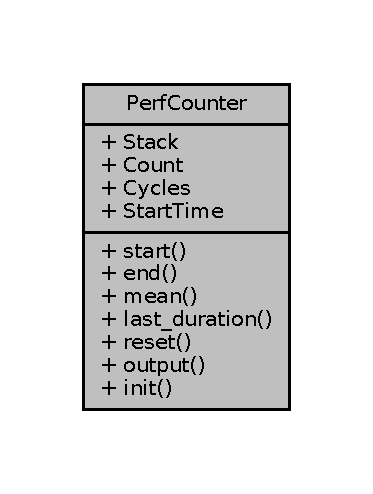
\includegraphics[width=179pt]{d3/dba/classPerfCounter__coll__graph}
\end{center}
\end{figure}
\subsection*{Public Member Functions}
\begin{DoxyCompactItemize}
\item 
void \hyperlink{classPerfCounter_a5fdd73c1d604decd6dc745aada8092d1}{start} () \+\_\+\+\_\+attribute\+\_\+\+\_\+((always\+\_\+inline))
\begin{DoxyCompactList}\small\item\em Start Measurement. \end{DoxyCompactList}\item 
void \hyperlink{classPerfCounter_ab5d9f05bb15139451eaa857989ed8bd8}{end} () \+\_\+\+\_\+attribute\+\_\+\+\_\+((always\+\_\+inline))
\begin{DoxyCompactList}\small\item\em End measurement. \end{DoxyCompactList}\item 
float \hyperlink{classPerfCounter_a5992367178f424e486a7709659e276a6}{mean} ()
\begin{DoxyCompactList}\small\item\em Returns the mean number of cycles between {\ttfamily \hyperlink{classPerfCounter_a5fdd73c1d604decd6dc745aada8092d1}{start()}} and {\ttfamily stop()}. \end{DoxyCompactList}\item 
uint32\+\_\+t \hyperlink{classPerfCounter_a5239f46d98a619e0145f09320052bfc8}{last\+\_\+duration} ()
\begin{DoxyCompactList}\small\item\em Returns the last recorded duration. \end{DoxyCompactList}\item 
void \hyperlink{classPerfCounter_a60f7428eabd82437280b662d6829e184}{reset} () \+\_\+\+\_\+attribute\+\_\+\+\_\+((always\+\_\+inline))
\item 
void \hyperlink{classPerfCounter_a291ce8187d35e1f97a68339fe51931a4}{output} () \+\_\+\+\_\+attribute\+\_\+\+\_\+((always\+\_\+inline))
\end{DoxyCompactItemize}
\subsection*{Static Public Member Functions}
\begin{DoxyCompactItemize}
\item 
static void \hyperlink{classPerfCounter_ae1897d617e84a28c141d554810fcaee9}{init} () \+\_\+\+\_\+attribute\+\_\+\+\_\+((always\+\_\+inline))
\begin{DoxyCompactList}\small\item\em Set up the debug module for clock cycle counting. \end{DoxyCompactList}\end{DoxyCompactItemize}
\subsection*{Public Attributes}
\begin{DoxyCompactItemize}
\item 
uint32\+\_\+t \hyperlink{classPerfCounter_ad440629d44a2bfd9b4d8de185ff66d27}{Stack} = 0
\begin{DoxyCompactList}\small\item\em Stack for mean calculation. \end{DoxyCompactList}\item 
uint32\+\_\+t \hyperlink{classPerfCounter_a8f86300240da2178dea60346ea72651c}{Count} = 0
\begin{DoxyCompactList}\small\item\em Count for mean calculation. \end{DoxyCompactList}\item 
uint32\+\_\+t \hyperlink{classPerfCounter_a60984f26cf145882c0355d28d8233e0a}{Cycles} = 0
\begin{DoxyCompactList}\small\item\em Last recorded duration (difference in clock cycles recorded) \end{DoxyCompactList}\item 
uint32\+\_\+t \hyperlink{classPerfCounter_adefe85b05d9c8920877053f6a8ed743c}{Start\+Time} = 0
\begin{DoxyCompactList}\small\item\em Stored starting time of the measurement. \end{DoxyCompactList}\end{DoxyCompactItemize}


\subsection{Detailed Description}
Performance Counter class for teensy 4.\+1 microcontrollers. 

\begin{DoxyNote}{Note}
{\ttfamily imxrt.\+h} defines {\ttfamily A\+R\+M\+\_\+\+D\+W\+T\+\_\+\+C\+Y\+C\+C\+NT} as {\ttfamily ($\ast$(volatile uint32\+\_\+t $\ast$)0x\+E0001004)}. 
\end{DoxyNote}


\subsection{Member Function Documentation}
\mbox{\Hypertarget{classPerfCounter_ab5d9f05bb15139451eaa857989ed8bd8}\label{classPerfCounter_ab5d9f05bb15139451eaa857989ed8bd8}} 
\index{Perf\+Counter@{Perf\+Counter}!end@{end}}
\index{end@{end}!Perf\+Counter@{Perf\+Counter}}
\subsubsection{\texorpdfstring{end()}{end()}}
{\footnotesize\ttfamily void Perf\+Counter\+::end (\begin{DoxyParamCaption}{ }\end{DoxyParamCaption})\hspace{0.3cm}{\ttfamily [inline]}}



End measurement. 

\mbox{\Hypertarget{classPerfCounter_ae1897d617e84a28c141d554810fcaee9}\label{classPerfCounter_ae1897d617e84a28c141d554810fcaee9}} 
\index{Perf\+Counter@{Perf\+Counter}!init@{init}}
\index{init@{init}!Perf\+Counter@{Perf\+Counter}}
\subsubsection{\texorpdfstring{init()}{init()}}
{\footnotesize\ttfamily static void Perf\+Counter\+::init (\begin{DoxyParamCaption}{ }\end{DoxyParamCaption})\hspace{0.3cm}{\ttfamily [inline]}, {\ttfamily [static]}}



Set up the debug module for clock cycle counting. 

\begin{DoxyWarning}{Warning}
This function sets the registers globally and will affect all instances and also the overall performance. 
\end{DoxyWarning}
\mbox{\Hypertarget{classPerfCounter_a5239f46d98a619e0145f09320052bfc8}\label{classPerfCounter_a5239f46d98a619e0145f09320052bfc8}} 
\index{Perf\+Counter@{Perf\+Counter}!last\+\_\+duration@{last\+\_\+duration}}
\index{last\+\_\+duration@{last\+\_\+duration}!Perf\+Counter@{Perf\+Counter}}
\subsubsection{\texorpdfstring{last\+\_\+duration()}{last\_duration()}}
{\footnotesize\ttfamily uint32\+\_\+t Perf\+Counter\+::last\+\_\+duration (\begin{DoxyParamCaption}{ }\end{DoxyParamCaption})\hspace{0.3cm}{\ttfamily [inline]}}



Returns the last recorded duration. 

\mbox{\Hypertarget{classPerfCounter_a5992367178f424e486a7709659e276a6}\label{classPerfCounter_a5992367178f424e486a7709659e276a6}} 
\index{Perf\+Counter@{Perf\+Counter}!mean@{mean}}
\index{mean@{mean}!Perf\+Counter@{Perf\+Counter}}
\subsubsection{\texorpdfstring{mean()}{mean()}}
{\footnotesize\ttfamily float Perf\+Counter\+::mean (\begin{DoxyParamCaption}{ }\end{DoxyParamCaption})\hspace{0.3cm}{\ttfamily [inline]}}



Returns the mean number of cycles between {\ttfamily \hyperlink{classPerfCounter_a5fdd73c1d604decd6dc745aada8092d1}{start()}} and {\ttfamily stop()}. 

\mbox{\Hypertarget{classPerfCounter_a291ce8187d35e1f97a68339fe51931a4}\label{classPerfCounter_a291ce8187d35e1f97a68339fe51931a4}} 
\index{Perf\+Counter@{Perf\+Counter}!output@{output}}
\index{output@{output}!Perf\+Counter@{Perf\+Counter}}
\subsubsection{\texorpdfstring{output()}{output()}}
{\footnotesize\ttfamily void Perf\+Counter\+::output (\begin{DoxyParamCaption}{ }\end{DoxyParamCaption})\hspace{0.3cm}{\ttfamily [inline]}}

\mbox{\Hypertarget{classPerfCounter_a60f7428eabd82437280b662d6829e184}\label{classPerfCounter_a60f7428eabd82437280b662d6829e184}} 
\index{Perf\+Counter@{Perf\+Counter}!reset@{reset}}
\index{reset@{reset}!Perf\+Counter@{Perf\+Counter}}
\subsubsection{\texorpdfstring{reset()}{reset()}}
{\footnotesize\ttfamily void Perf\+Counter\+::reset (\begin{DoxyParamCaption}{ }\end{DoxyParamCaption})\hspace{0.3cm}{\ttfamily [inline]}}

\mbox{\Hypertarget{classPerfCounter_a5fdd73c1d604decd6dc745aada8092d1}\label{classPerfCounter_a5fdd73c1d604decd6dc745aada8092d1}} 
\index{Perf\+Counter@{Perf\+Counter}!start@{start}}
\index{start@{start}!Perf\+Counter@{Perf\+Counter}}
\subsubsection{\texorpdfstring{start()}{start()}}
{\footnotesize\ttfamily void Perf\+Counter\+::start (\begin{DoxyParamCaption}{ }\end{DoxyParamCaption})\hspace{0.3cm}{\ttfamily [inline]}}



Start Measurement. 



\subsection{Member Data Documentation}
\mbox{\Hypertarget{classPerfCounter_a8f86300240da2178dea60346ea72651c}\label{classPerfCounter_a8f86300240da2178dea60346ea72651c}} 
\index{Perf\+Counter@{Perf\+Counter}!Count@{Count}}
\index{Count@{Count}!Perf\+Counter@{Perf\+Counter}}
\subsubsection{\texorpdfstring{Count}{Count}}
{\footnotesize\ttfamily uint32\+\_\+t Perf\+Counter\+::\+Count = 0}



Count for mean calculation. 

\mbox{\Hypertarget{classPerfCounter_a60984f26cf145882c0355d28d8233e0a}\label{classPerfCounter_a60984f26cf145882c0355d28d8233e0a}} 
\index{Perf\+Counter@{Perf\+Counter}!Cycles@{Cycles}}
\index{Cycles@{Cycles}!Perf\+Counter@{Perf\+Counter}}
\subsubsection{\texorpdfstring{Cycles}{Cycles}}
{\footnotesize\ttfamily uint32\+\_\+t Perf\+Counter\+::\+Cycles = 0}



Last recorded duration (difference in clock cycles recorded) 

\mbox{\Hypertarget{classPerfCounter_ad440629d44a2bfd9b4d8de185ff66d27}\label{classPerfCounter_ad440629d44a2bfd9b4d8de185ff66d27}} 
\index{Perf\+Counter@{Perf\+Counter}!Stack@{Stack}}
\index{Stack@{Stack}!Perf\+Counter@{Perf\+Counter}}
\subsubsection{\texorpdfstring{Stack}{Stack}}
{\footnotesize\ttfamily uint32\+\_\+t Perf\+Counter\+::\+Stack = 0}



Stack for mean calculation. 

\mbox{\Hypertarget{classPerfCounter_adefe85b05d9c8920877053f6a8ed743c}\label{classPerfCounter_adefe85b05d9c8920877053f6a8ed743c}} 
\index{Perf\+Counter@{Perf\+Counter}!Start\+Time@{Start\+Time}}
\index{Start\+Time@{Start\+Time}!Perf\+Counter@{Perf\+Counter}}
\subsubsection{\texorpdfstring{Start\+Time}{StartTime}}
{\footnotesize\ttfamily uint32\+\_\+t Perf\+Counter\+::\+Start\+Time = 0}



Stored starting time of the measurement. 



The documentation for this class was generated from the following file\+:\begin{DoxyCompactItemize}
\item 
code/hardware/\hyperlink{perf__counter_8hpp}{perf\+\_\+counter.\+hpp}\end{DoxyCompactItemize}

\hypertarget{classPIT__LifetimeTimer}{}\section{P\+I\+T\+\_\+\+Lifetime\+Timer Class Reference}
\label{classPIT__LifetimeTimer}\index{P\+I\+T\+\_\+\+Lifetime\+Timer@{P\+I\+T\+\_\+\+Lifetime\+Timer}}


Interface for using the \char`\"{}\+Life Time T\+Imer\char`\"{} functionality of the Periodic Interrut Timer on Teensy 4.\+x microcontrollers. The module uses Channel 0 and 1 of the 4 P\+IT channels.  




{\ttfamily \#include $<$lifetime\+\_\+timer.\+hpp$>$}

\subsection*{Public Member Functions}
\begin{DoxyCompactItemize}
\item 
\hyperlink{classPIT__LifetimeTimer_a826797e75688ab4e7cd5c8854fa6a7c0}{P\+I\+T\+\_\+\+Lifetime\+Timer} ()
\item 
void \hyperlink{classPIT__LifetimeTimer_ad1c585d138123be94769afcca87f2dc6}{init} () \+\_\+\+\_\+attribute\+\_\+\+\_\+((always\+\_\+inline))
\begin{DoxyCompactList}\small\item\em Sets up Timer 0 and Timer 1 channels for Lifetime timing -\/ chained configuration. This function also makes a call to enable P\+IT timers. The timers are aet at maximum values and will start downcounting once \hyperlink{classPIT__LifetimeTimer_a6feabeff2529cabaf27ef53d027a4fc9}{P\+I\+T\+\_\+\+Lifetime\+Timer\+::start()} method is called. \end{DoxyCompactList}\item 
void \hyperlink{classPIT__LifetimeTimer_a6feabeff2529cabaf27ef53d027a4fc9}{start} () \+\_\+\+\_\+attribute\+\_\+\+\_\+((always\+\_\+inline))
\begin{DoxyCompactList}\small\item\em Starts the timers for down counting. \end{DoxyCompactList}\item 
void \hyperlink{classPIT__LifetimeTimer_a92543f292044725b1dea4d009e01d9e4}{stop} () \+\_\+\+\_\+attribute\+\_\+\+\_\+((always\+\_\+inline))
\begin{DoxyCompactList}\small\item\em Stops the timers from counting. The timers values will freeze. \end{DoxyCompactList}\item 
void \hyperlink{classPIT__LifetimeTimer_a5c1c38cfa6c7a049a495ee3d89e13276}{reset} () \+\_\+\+\_\+attribute\+\_\+\+\_\+((always\+\_\+inline))
\begin{DoxyCompactList}\small\item\em Stops the timers and resets the timer back to the init value (max) -\/ 0x\+F\+F\+F\+F\+F\+F\+F\+F\+F\+F\+F\+F\+FF. \end{DoxyCompactList}\item 
uint64\+\_\+t \hyperlink{classPIT__LifetimeTimer_a4ee08cce7812322a7a10fcba0463476c}{read\+\_\+val} () \+\_\+\+\_\+attribute\+\_\+\+\_\+((always\+\_\+inline))
\begin{DoxyCompactList}\small\item\em Returns the complete 64-\/bit timing value. \end{DoxyCompactList}\item 
uint32\+\_\+t \hyperlink{classPIT__LifetimeTimer_a4f7f8cd3847b9edb19dfa27f048a08cc}{read\+\_\+low\+\_\+val} () \+\_\+\+\_\+attribute\+\_\+\+\_\+((always\+\_\+inline))
\begin{DoxyCompactList}\small\item\em Returns the lower 32-\/bit half of the 64-\/bit timing value. \end{DoxyCompactList}\item 
uint32\+\_\+t \hyperlink{classPIT__LifetimeTimer_a39b0861ac88aec5e53f326409d536bcf}{read\+\_\+high\+\_\+val} () \+\_\+\+\_\+attribute\+\_\+\+\_\+((always\+\_\+inline))
\begin{DoxyCompactList}\small\item\em Returns the higher 32-\/bit half of the 64-\/bit timing value. \end{DoxyCompactList}\item 
uint64\+\_\+t \hyperlink{classPIT__LifetimeTimer_a04adf2272a47d4c81a28c6363e2da4fd}{elapsed64} () \+\_\+\+\_\+attribute\+\_\+\+\_\+((always\+\_\+inline))
\begin{DoxyCompactList}\small\item\em Returns the elapsed duration from the start call of the timer. The return is the complete 64bit value. \end{DoxyCompactList}\item 
uint32\+\_\+t \hyperlink{classPIT__LifetimeTimer_af7481214070333f845a23456b4d75880}{elapsed32} () \+\_\+\+\_\+attribute\+\_\+\+\_\+((always\+\_\+inline))
\begin{DoxyCompactList}\small\item\em Returns the elapsed duration from the start call of the timer. The return is the lower 32-\/bit half elapsed time value. \end{DoxyCompactList}\end{DoxyCompactItemize}


\subsection{Detailed Description}
Interface for using the \char`\"{}\+Life Time T\+Imer\char`\"{} functionality of the Periodic Interrut Timer on Teensy 4.\+x microcontrollers. The module uses Channel 0 and 1 of the 4 P\+IT channels. 

\begin{DoxyAttention}{Attention}
The module has no checks on the use of C\+H0 and C\+H1 by external drivers, however, the interface enforces a singleton template and can only be constructed once. 

The module does not set the clock frequency and uses either the default or the one set globally (as is the only use case) by external drivers outside its scope. 

Source \+: Code adapted from I\+M\+X\+RT Manual Page 2977. 
\end{DoxyAttention}
\begin{DoxyRefDesc}{Todo}
\item[\hyperlink{todo__todo000002}{Todo}]Resolve Singleton template -\/ constexpr static issue. \end{DoxyRefDesc}


\subsection{Constructor \& Destructor Documentation}
\mbox{\Hypertarget{classPIT__LifetimeTimer_a826797e75688ab4e7cd5c8854fa6a7c0}\label{classPIT__LifetimeTimer_a826797e75688ab4e7cd5c8854fa6a7c0}} 
\index{P\+I\+T\+\_\+\+Lifetime\+Timer@{P\+I\+T\+\_\+\+Lifetime\+Timer}!P\+I\+T\+\_\+\+Lifetime\+Timer@{P\+I\+T\+\_\+\+Lifetime\+Timer}}
\index{P\+I\+T\+\_\+\+Lifetime\+Timer@{P\+I\+T\+\_\+\+Lifetime\+Timer}!P\+I\+T\+\_\+\+Lifetime\+Timer@{P\+I\+T\+\_\+\+Lifetime\+Timer}}
\subsubsection{\texorpdfstring{P\+I\+T\+\_\+\+Lifetime\+Timer()}{PIT\_LifetimeTimer()}}
{\footnotesize\ttfamily P\+I\+T\+\_\+\+Lifetime\+Timer\+::\+P\+I\+T\+\_\+\+Lifetime\+Timer (\begin{DoxyParamCaption}{ }\end{DoxyParamCaption})\hspace{0.3cm}{\ttfamily [inline]}}



\subsection{Member Function Documentation}
\mbox{\Hypertarget{classPIT__LifetimeTimer_af7481214070333f845a23456b4d75880}\label{classPIT__LifetimeTimer_af7481214070333f845a23456b4d75880}} 
\index{P\+I\+T\+\_\+\+Lifetime\+Timer@{P\+I\+T\+\_\+\+Lifetime\+Timer}!elapsed32@{elapsed32}}
\index{elapsed32@{elapsed32}!P\+I\+T\+\_\+\+Lifetime\+Timer@{P\+I\+T\+\_\+\+Lifetime\+Timer}}
\subsubsection{\texorpdfstring{elapsed32()}{elapsed32()}}
{\footnotesize\ttfamily uint32\+\_\+t P\+I\+T\+\_\+\+Lifetime\+Timer\+::elapsed32 (\begin{DoxyParamCaption}{ }\end{DoxyParamCaption})\hspace{0.3cm}{\ttfamily [inline]}}



Returns the elapsed duration from the start call of the timer. The return is the lower 32-\/bit half elapsed time value. 

\begin{DoxyWarning}{Warning}
If the elapsed duration is greater than the 32-\/bit rollover time, then the quantity returned is meaningless. Hence, use of this function should be reserved for measuring small time durarions. 
\end{DoxyWarning}
\mbox{\Hypertarget{classPIT__LifetimeTimer_a04adf2272a47d4c81a28c6363e2da4fd}\label{classPIT__LifetimeTimer_a04adf2272a47d4c81a28c6363e2da4fd}} 
\index{P\+I\+T\+\_\+\+Lifetime\+Timer@{P\+I\+T\+\_\+\+Lifetime\+Timer}!elapsed64@{elapsed64}}
\index{elapsed64@{elapsed64}!P\+I\+T\+\_\+\+Lifetime\+Timer@{P\+I\+T\+\_\+\+Lifetime\+Timer}}
\subsubsection{\texorpdfstring{elapsed64()}{elapsed64()}}
{\footnotesize\ttfamily uint64\+\_\+t P\+I\+T\+\_\+\+Lifetime\+Timer\+::elapsed64 (\begin{DoxyParamCaption}{ }\end{DoxyParamCaption})\hspace{0.3cm}{\ttfamily [inline]}}



Returns the elapsed duration from the start call of the timer. The return is the complete 64bit value. 

\mbox{\Hypertarget{classPIT__LifetimeTimer_ad1c585d138123be94769afcca87f2dc6}\label{classPIT__LifetimeTimer_ad1c585d138123be94769afcca87f2dc6}} 
\index{P\+I\+T\+\_\+\+Lifetime\+Timer@{P\+I\+T\+\_\+\+Lifetime\+Timer}!init@{init}}
\index{init@{init}!P\+I\+T\+\_\+\+Lifetime\+Timer@{P\+I\+T\+\_\+\+Lifetime\+Timer}}
\subsubsection{\texorpdfstring{init()}{init()}}
{\footnotesize\ttfamily void P\+I\+T\+\_\+\+Lifetime\+Timer\+::init (\begin{DoxyParamCaption}{ }\end{DoxyParamCaption})\hspace{0.3cm}{\ttfamily [inline]}}



Sets up Timer 0 and Timer 1 channels for Lifetime timing -\/ chained configuration. This function also makes a call to enable P\+IT timers. The timers are aet at maximum values and will start downcounting once \hyperlink{classPIT__LifetimeTimer_a6feabeff2529cabaf27ef53d027a4fc9}{P\+I\+T\+\_\+\+Lifetime\+Timer\+::start()} method is called. 

\begin{DoxyAttention}{Attention}
Reference \+: Code adapted from I\+M\+X\+RT Manual Page 2977. 

The timers will operate at the clock frequency set for P\+IT timers outside this library. 
\end{DoxyAttention}
\mbox{\Hypertarget{classPIT__LifetimeTimer_a39b0861ac88aec5e53f326409d536bcf}\label{classPIT__LifetimeTimer_a39b0861ac88aec5e53f326409d536bcf}} 
\index{P\+I\+T\+\_\+\+Lifetime\+Timer@{P\+I\+T\+\_\+\+Lifetime\+Timer}!read\+\_\+high\+\_\+val@{read\+\_\+high\+\_\+val}}
\index{read\+\_\+high\+\_\+val@{read\+\_\+high\+\_\+val}!P\+I\+T\+\_\+\+Lifetime\+Timer@{P\+I\+T\+\_\+\+Lifetime\+Timer}}
\subsubsection{\texorpdfstring{read\+\_\+high\+\_\+val()}{read\_high\_val()}}
{\footnotesize\ttfamily uint32\+\_\+t P\+I\+T\+\_\+\+Lifetime\+Timer\+::read\+\_\+high\+\_\+val (\begin{DoxyParamCaption}{ }\end{DoxyParamCaption})\hspace{0.3cm}{\ttfamily [inline]}}



Returns the higher 32-\/bit half of the 64-\/bit timing value. 

\mbox{\Hypertarget{classPIT__LifetimeTimer_a4f7f8cd3847b9edb19dfa27f048a08cc}\label{classPIT__LifetimeTimer_a4f7f8cd3847b9edb19dfa27f048a08cc}} 
\index{P\+I\+T\+\_\+\+Lifetime\+Timer@{P\+I\+T\+\_\+\+Lifetime\+Timer}!read\+\_\+low\+\_\+val@{read\+\_\+low\+\_\+val}}
\index{read\+\_\+low\+\_\+val@{read\+\_\+low\+\_\+val}!P\+I\+T\+\_\+\+Lifetime\+Timer@{P\+I\+T\+\_\+\+Lifetime\+Timer}}
\subsubsection{\texorpdfstring{read\+\_\+low\+\_\+val()}{read\_low\_val()}}
{\footnotesize\ttfamily uint32\+\_\+t P\+I\+T\+\_\+\+Lifetime\+Timer\+::read\+\_\+low\+\_\+val (\begin{DoxyParamCaption}{ }\end{DoxyParamCaption})\hspace{0.3cm}{\ttfamily [inline]}}



Returns the lower 32-\/bit half of the 64-\/bit timing value. 

\mbox{\Hypertarget{classPIT__LifetimeTimer_a4ee08cce7812322a7a10fcba0463476c}\label{classPIT__LifetimeTimer_a4ee08cce7812322a7a10fcba0463476c}} 
\index{P\+I\+T\+\_\+\+Lifetime\+Timer@{P\+I\+T\+\_\+\+Lifetime\+Timer}!read\+\_\+val@{read\+\_\+val}}
\index{read\+\_\+val@{read\+\_\+val}!P\+I\+T\+\_\+\+Lifetime\+Timer@{P\+I\+T\+\_\+\+Lifetime\+Timer}}
\subsubsection{\texorpdfstring{read\+\_\+val()}{read\_val()}}
{\footnotesize\ttfamily uint64\+\_\+t P\+I\+T\+\_\+\+Lifetime\+Timer\+::read\+\_\+val (\begin{DoxyParamCaption}{ }\end{DoxyParamCaption})\hspace{0.3cm}{\ttfamily [inline]}}



Returns the complete 64-\/bit timing value. 

\mbox{\Hypertarget{classPIT__LifetimeTimer_a5c1c38cfa6c7a049a495ee3d89e13276}\label{classPIT__LifetimeTimer_a5c1c38cfa6c7a049a495ee3d89e13276}} 
\index{P\+I\+T\+\_\+\+Lifetime\+Timer@{P\+I\+T\+\_\+\+Lifetime\+Timer}!reset@{reset}}
\index{reset@{reset}!P\+I\+T\+\_\+\+Lifetime\+Timer@{P\+I\+T\+\_\+\+Lifetime\+Timer}}
\subsubsection{\texorpdfstring{reset()}{reset()}}
{\footnotesize\ttfamily void P\+I\+T\+\_\+\+Lifetime\+Timer\+::reset (\begin{DoxyParamCaption}{ }\end{DoxyParamCaption})\hspace{0.3cm}{\ttfamily [inline]}}



Stops the timers and resets the timer back to the init value (max) -\/ 0x\+F\+F\+F\+F\+F\+F\+F\+F\+F\+F\+F\+F\+FF. 

\mbox{\Hypertarget{classPIT__LifetimeTimer_a6feabeff2529cabaf27ef53d027a4fc9}\label{classPIT__LifetimeTimer_a6feabeff2529cabaf27ef53d027a4fc9}} 
\index{P\+I\+T\+\_\+\+Lifetime\+Timer@{P\+I\+T\+\_\+\+Lifetime\+Timer}!start@{start}}
\index{start@{start}!P\+I\+T\+\_\+\+Lifetime\+Timer@{P\+I\+T\+\_\+\+Lifetime\+Timer}}
\subsubsection{\texorpdfstring{start()}{start()}}
{\footnotesize\ttfamily void P\+I\+T\+\_\+\+Lifetime\+Timer\+::start (\begin{DoxyParamCaption}{ }\end{DoxyParamCaption})\hspace{0.3cm}{\ttfamily [inline]}}



Starts the timers for down counting. 

\mbox{\Hypertarget{classPIT__LifetimeTimer_a92543f292044725b1dea4d009e01d9e4}\label{classPIT__LifetimeTimer_a92543f292044725b1dea4d009e01d9e4}} 
\index{P\+I\+T\+\_\+\+Lifetime\+Timer@{P\+I\+T\+\_\+\+Lifetime\+Timer}!stop@{stop}}
\index{stop@{stop}!P\+I\+T\+\_\+\+Lifetime\+Timer@{P\+I\+T\+\_\+\+Lifetime\+Timer}}
\subsubsection{\texorpdfstring{stop()}{stop()}}
{\footnotesize\ttfamily void P\+I\+T\+\_\+\+Lifetime\+Timer\+::stop (\begin{DoxyParamCaption}{ }\end{DoxyParamCaption})\hspace{0.3cm}{\ttfamily [inline]}}



Stops the timers from counting. The timers values will freeze. 



The documentation for this class was generated from the following file\+:\begin{DoxyCompactItemize}
\item 
code/hardware/\hyperlink{lifetime__timer_8hpp}{lifetime\+\_\+timer.\+hpp}\end{DoxyCompactItemize}

\hypertarget{classPITController}{}\section{P\+I\+T\+Controller$<$ Ch\+ID $>$ Class Template Reference}
\label{classPITController}\index{P\+I\+T\+Controller$<$ Ch\+I\+D $>$@{P\+I\+T\+Controller$<$ Ch\+I\+D $>$}}


Interface for P\+IT timers on Teensy 4.\+x microcontrollers.  




{\ttfamily \#include $<$pit.\+hpp$>$}

\subsection*{Public Member Functions}
\begin{DoxyCompactItemize}
\item 
\hyperlink{classPITController_ad9ef4f151495076fad7b0c556e48b117}{P\+I\+T\+Controller} ()
\begin{DoxyCompactList}\small\item\em Constant -\/ Maximum possible counter value. 32 bit counter. \end{DoxyCompactList}\item 
void \hyperlink{group__Controls_ga4dae1ed0ada64ebc03665e8f39795e7e}{start} () \hyperlink{utilities_8hpp_a103d5b3998e0dd804213c8f30a094f4d}{\+\_\+\+\_\+attribute\+\_\+\+\_\+}((always\+\_\+inline))
\begin{DoxyCompactList}\small\item\em Start counting on the timer. \end{DoxyCompactList}\item 
void \hyperlink{group__Controls_ga5a6e2b00c6355934531a77a62660bec7}{stop} () \hyperlink{utilities_8hpp_a103d5b3998e0dd804213c8f30a094f4d}{\+\_\+\+\_\+attribute\+\_\+\+\_\+}((always\+\_\+inline))
\begin{DoxyCompactList}\small\item\em stop counting on the timer. \end{DoxyCompactList}\item 
\hyperlink{errors_8hpp_a4e8c0d09726859e3d3369c0da5a1aa7f}{Error\+\_\+t} \hyperlink{group__Controls_gaaf7a79129a4ea5af057ea8f537b7ae9f}{set\+\_\+gate\+\_\+time} (double gt\+\_\+microseconds) \hyperlink{utilities_8hpp_a103d5b3998e0dd804213c8f30a094f4d}{\+\_\+\+\_\+attribute\+\_\+\+\_\+}((flatten))
\begin{DoxyCompactList}\small\item\em Sets the gate time after which the counter returns to zero and marks the end of onegate interval. \end{DoxyCompactList}\item 
double \hyperlink{group__Controls_ga3fedb5ff5a44b664e8132f4e2836b155}{period\+\_\+error\+\_\+us} () const \hyperlink{utilities_8hpp_a103d5b3998e0dd804213c8f30a094f4d}{\+\_\+\+\_\+attribute\+\_\+\+\_\+}((always\+\_\+inline))
\begin{DoxyCompactList}\small\item\em Returns the error in the gate timing period due to the finite resolution of the timers.  Error in microseconds. \end{DoxyCompactList}\item 
double \hyperlink{group__Controls_ga2b64ce8a01dc1254002c4ff3c384a6fd}{tick\+\_\+period\+\_\+us} () \hyperlink{utilities_8hpp_a103d5b3998e0dd804213c8f30a094f4d}{\+\_\+\+\_\+attribute\+\_\+\+\_\+}((always\+\_\+inline))
\begin{DoxyCompactList}\small\item\em Returns the value of one {\bfseries Tick} -\/ Minimum resolution of the timer. \end{DoxyCompactList}\item 
void \hyperlink{group__Controls_ga19f11a8cdb94353ffaaa5a2eccf35ee5}{get\+\_\+xbar\+\_\+in\+\_\+pin} () \hyperlink{utilities_8hpp_a103d5b3998e0dd804213c8f30a094f4d}{\+\_\+\+\_\+attribute\+\_\+\+\_\+}((always\+\_\+inline))
\begin{DoxyCompactList}\small\item\em Returns the correspoding X\+B\+A\+R1-\/A Input Pins for the corresponding channel T\+R\+I\+G\+G\+ER signal.  -\/ Manual Page 63. \end{DoxyCompactList}\item 
void \hyperlink{group__Interrupt_gaf1a21e0b3f9a57e247aa40c457e15ee3}{interrupt} () \hyperlink{utilities_8hpp_a103d5b3998e0dd804213c8f30a094f4d}{\+\_\+\+\_\+attribute\+\_\+\+\_\+}((always\+\_\+inline))
\begin{DoxyCompactList}\small\item\em Enable Interruptsthat are triggered after one gate time completion. \end{DoxyCompactList}\item 
void \hyperlink{group__Interrupt_ga6e36c84f319e52e5a14ca20f299b64b5}{no\+\_\+interrupt} () \hyperlink{utilities_8hpp_a103d5b3998e0dd804213c8f30a094f4d}{\+\_\+\+\_\+attribute\+\_\+\+\_\+}((always\+\_\+inline))
\begin{DoxyCompactList}\small\item\em Disable Interrupts that are triggered after one gate time completion. \end{DoxyCompactList}\item 
void \hyperlink{group__Interrupt_gae3f9c981e88cced34153234475de5646}{clear\+\_\+interrupt\+\_\+flag} () \hyperlink{utilities_8hpp_a103d5b3998e0dd804213c8f30a094f4d}{\+\_\+\+\_\+attribute\+\_\+\+\_\+}((always\+\_\+inline))
\begin{DoxyCompactList}\small\item\em Clears the interrupt flag and hence prepares the timer for the next gate interval. The clearing has to be done manually. If the flag is not cleared, the interrupt will be called again and again. \end{DoxyCompactList}\item 
void \hyperlink{group__CLK_ga63e67e2ebfd6ceb5f5e38d9bd6a54754}{sel\+\_\+\+F\+B\+U\+S\+\_\+clock} () \hyperlink{utilities_8hpp_a103d5b3998e0dd804213c8f30a094f4d}{\+\_\+\+\_\+attribute\+\_\+\+\_\+}((always\+\_\+inline))
\begin{DoxyCompactList}\small\item\em Sets the clock source frequency of all P\+IT channels to the value F\+\_\+\+B\+U\+S\+\_\+\+A\+C\+T\+U\+AL (= F\+\_\+\+C\+P\+U\+\_\+\+A\+C\+T\+U\+AL / 4 ) which is nominally 150 M\+Hz. The exact value depends on the C\+PU clock rate. \end{DoxyCompactList}\item 
void \hyperlink{group__CLK_gadb0d04fa23f4ebd20d2f495a86af3ccd}{sel\+\_\+24\+M\+Hz\+\_\+clock} () \hyperlink{utilities_8hpp_a103d5b3998e0dd804213c8f30a094f4d}{\+\_\+\+\_\+attribute\+\_\+\+\_\+}((always\+\_\+inline))
\begin{DoxyCompactList}\small\item\em Sets the source clock frequency of all P\+IT channels to 24 M\+Hz which is the default oscillator clock. This setting is also the default state, if no clock is selected. \end{DoxyCompactList}\end{DoxyCompactItemize}
\subsection*{Static Public Member Functions}
\begin{DoxyCompactItemize}
\item 
static void \hyperlink{group__PIT__Glb_gaa742977692efbc075b52a5dbd6533230}{enable\+\_\+\+P\+I\+Ts} () \hyperlink{utilities_8hpp_a103d5b3998e0dd804213c8f30a094f4d}{\+\_\+\+\_\+attribute\+\_\+\+\_\+}((always\+\_\+inline))
\begin{DoxyCompactList}\small\item\em Enable all P\+IT channels. \end{DoxyCompactList}\item 
static void \hyperlink{group__PIT__Glb_ga5e1bf9f8053a51c68f0ff2178ab56954}{disable\+\_\+\+P\+I\+Ts} () \hyperlink{utilities_8hpp_a103d5b3998e0dd804213c8f30a094f4d}{\+\_\+\+\_\+attribute\+\_\+\+\_\+}((always\+\_\+inline))
\begin{DoxyCompactList}\small\item\em Disable all P\+IT Channels. \end{DoxyCompactList}\item 
static void \hyperlink{group__PIT__Glb_ga24b7ea02555967ef945ab87aae338574}{pause\+\_\+resume\+\_\+\+P\+I\+Ts} () \hyperlink{utilities_8hpp_a103d5b3998e0dd804213c8f30a094f4d}{\+\_\+\+\_\+attribute\+\_\+\+\_\+}((always\+\_\+inline))
\begin{DoxyCompactList}\small\item\em Pause/\+Resume -\/ {\bfseries Toggle} all P\+IT Channels. \end{DoxyCompactList}\item 
static void \hyperlink{group__Interrupt_gaa94b6dc081d453c8dda54c3ade4b3d94}{set\+\_\+interrupt} (void($\ast$isr\+\_\+fn)(), unsigned int priority) \hyperlink{utilities_8hpp_a103d5b3998e0dd804213c8f30a094f4d}{\+\_\+\+\_\+attribute\+\_\+\+\_\+}((always\+\_\+inline))
\begin{DoxyCompactList}\small\item\em Sets a common I\+SR and its priority for all P\+IT Channels. \end{DoxyCompactList}\end{DoxyCompactItemize}
\subsection*{Public Attributes}
\begin{DoxyCompactItemize}
\item 
double \hyperlink{classPITController_a549601e7c66941d7872a6e7d38ed9563}{Actual\+\_\+period} = 0
\item 
double \hyperlink{classPITController_a9de0af49a52145c8d2a8f4e90a519b60}{Req\+\_\+period} = 0
\begin{DoxyCompactList}\small\item\em Actual Time Period set by the device due to finite resolution. \end{DoxyCompactList}\item 
uint32\+\_\+t \hyperlink{classPITController_ae3d74bb18e5b22769e895f592cb16129}{Clk\+\_\+freq} = uint32\+\_\+t(24 $\ast$ 1e6)
\begin{DoxyCompactList}\small\item\em Time Period requested by the user. \end{DoxyCompactList}\end{DoxyCompactItemize}
\subsection*{Static Public Attributes}
\begin{DoxyCompactItemize}
\item 
static const constexpr uint32\+\_\+t \hyperlink{classPITController_a53778fe7e47ac9741bef0bc190e0646a}{P\+I\+T\+\_\+\+M\+A\+X\+\_\+\+C\+O\+U\+N\+T\+ER} = 4294967295
\begin{DoxyCompactList}\small\item\em Clock frequency used by the timer. Initalized to 24\+M\+Hz → default oscillator clock. \end{DoxyCompactList}\end{DoxyCompactItemize}


\subsection{Detailed Description}
\subsubsection*{template$<$unsigned int Ch\+ID$>$\newline
class P\+I\+T\+Controller$<$ Ch\+I\+D $>$}

Interface for P\+IT timers on Teensy 4.\+x microcontrollers. 

\subsection{Constructor \& Destructor Documentation}
\mbox{\Hypertarget{classPITController_ad9ef4f151495076fad7b0c556e48b117}\label{classPITController_ad9ef4f151495076fad7b0c556e48b117}} 
\index{P\+I\+T\+Controller@{P\+I\+T\+Controller}!P\+I\+T\+Controller@{P\+I\+T\+Controller}}
\index{P\+I\+T\+Controller@{P\+I\+T\+Controller}!P\+I\+T\+Controller@{P\+I\+T\+Controller}}
\subsubsection{\texorpdfstring{P\+I\+T\+Controller()}{PITController()}}
{\footnotesize\ttfamily template$<$unsigned int Ch\+ID$>$ \\
\hyperlink{classPITController}{P\+I\+T\+Controller}$<$ Ch\+ID $>$\+::\hyperlink{classPITController}{P\+I\+T\+Controller} (\begin{DoxyParamCaption}{ }\end{DoxyParamCaption})\hspace{0.3cm}{\ttfamily [inline]}}



Constant -\/ Maximum possible counter value. 32 bit counter. 



\subsection{Member Data Documentation}
\mbox{\Hypertarget{classPITController_a549601e7c66941d7872a6e7d38ed9563}\label{classPITController_a549601e7c66941d7872a6e7d38ed9563}} 
\index{P\+I\+T\+Controller@{P\+I\+T\+Controller}!Actual\+\_\+period@{Actual\+\_\+period}}
\index{Actual\+\_\+period@{Actual\+\_\+period}!P\+I\+T\+Controller@{P\+I\+T\+Controller}}
\subsubsection{\texorpdfstring{Actual\+\_\+period}{Actual\_period}}
{\footnotesize\ttfamily template$<$unsigned int Ch\+ID$>$ \\
double \hyperlink{classPITController}{P\+I\+T\+Controller}$<$ Ch\+ID $>$\+::Actual\+\_\+period = 0}

\mbox{\Hypertarget{classPITController_ae3d74bb18e5b22769e895f592cb16129}\label{classPITController_ae3d74bb18e5b22769e895f592cb16129}} 
\index{P\+I\+T\+Controller@{P\+I\+T\+Controller}!Clk\+\_\+freq@{Clk\+\_\+freq}}
\index{Clk\+\_\+freq@{Clk\+\_\+freq}!P\+I\+T\+Controller@{P\+I\+T\+Controller}}
\subsubsection{\texorpdfstring{Clk\+\_\+freq}{Clk\_freq}}
{\footnotesize\ttfamily template$<$unsigned int Ch\+ID$>$ \\
uint32\+\_\+t \hyperlink{classPITController}{P\+I\+T\+Controller}$<$ Ch\+ID $>$\+::Clk\+\_\+freq = uint32\+\_\+t(24 $\ast$ 1e6)}



Time Period requested by the user. 

\mbox{\Hypertarget{classPITController_a53778fe7e47ac9741bef0bc190e0646a}\label{classPITController_a53778fe7e47ac9741bef0bc190e0646a}} 
\index{P\+I\+T\+Controller@{P\+I\+T\+Controller}!P\+I\+T\+\_\+\+M\+A\+X\+\_\+\+C\+O\+U\+N\+T\+ER@{P\+I\+T\+\_\+\+M\+A\+X\+\_\+\+C\+O\+U\+N\+T\+ER}}
\index{P\+I\+T\+\_\+\+M\+A\+X\+\_\+\+C\+O\+U\+N\+T\+ER@{P\+I\+T\+\_\+\+M\+A\+X\+\_\+\+C\+O\+U\+N\+T\+ER}!P\+I\+T\+Controller@{P\+I\+T\+Controller}}
\subsubsection{\texorpdfstring{P\+I\+T\+\_\+\+M\+A\+X\+\_\+\+C\+O\+U\+N\+T\+ER}{PIT\_MAX\_COUNTER}}
{\footnotesize\ttfamily template$<$unsigned int Ch\+ID$>$ \\
const constexpr uint32\+\_\+t \hyperlink{classPITController}{P\+I\+T\+Controller}$<$ Ch\+ID $>$\+::P\+I\+T\+\_\+\+M\+A\+X\+\_\+\+C\+O\+U\+N\+T\+ER = 4294967295\hspace{0.3cm}{\ttfamily [static]}}



Clock frequency used by the timer. Initalized to 24\+M\+Hz → default oscillator clock. 

\mbox{\Hypertarget{classPITController_a9de0af49a52145c8d2a8f4e90a519b60}\label{classPITController_a9de0af49a52145c8d2a8f4e90a519b60}} 
\index{P\+I\+T\+Controller@{P\+I\+T\+Controller}!Req\+\_\+period@{Req\+\_\+period}}
\index{Req\+\_\+period@{Req\+\_\+period}!P\+I\+T\+Controller@{P\+I\+T\+Controller}}
\subsubsection{\texorpdfstring{Req\+\_\+period}{Req\_period}}
{\footnotesize\ttfamily template$<$unsigned int Ch\+ID$>$ \\
double \hyperlink{classPITController}{P\+I\+T\+Controller}$<$ Ch\+ID $>$\+::Req\+\_\+period = 0}



Actual Time Period set by the device due to finite resolution. 



The documentation for this class was generated from the following file\+:\begin{DoxyCompactItemize}
\item 
/mnt/m/code/\+Correlator/\hyperlink{pit_8hpp}{pit.\+hpp}\end{DoxyCompactItemize}

\hypertarget{classlive__graph_1_1PStatLiveGraph}{}\section{live\+\_\+graph.\+P\+Stat\+Live\+Graph Class Reference}
\label{classlive__graph_1_1PStatLiveGraph}\index{live\+\_\+graph.\+P\+Stat\+Live\+Graph@{live\+\_\+graph.\+P\+Stat\+Live\+Graph}}
\subsection*{Public Member Functions}
\begin{DoxyCompactItemize}
\item 
def \hyperlink{classlive__graph_1_1PStatLiveGraph_a210a499fd4e06392f8f5fffc209971a4}{\+\_\+\+\_\+init\+\_\+\+\_\+} (self, port=None)
\item 
def \hyperlink{classlive__graph_1_1PStatLiveGraph_a65b6193384abea9656044a84a6112eb2}{init\+\_\+plots} (config)
\item 
def \hyperlink{classlive__graph_1_1PStatLiveGraph_a7730f214090df612485e42ae758beb3e}{screen\+\_\+size\+\_\+calc} (final\+\_\+row, final\+\_\+col)
\item 
def \hyperlink{classlive__graph_1_1PStatLiveGraph_a4969c53cd50f31c9b50d86a7cac77a63}{grid\+\_\+allocator} (halfcol=False)
\item 
def \hyperlink{classlive__graph_1_1PStatLiveGraph_af167003562729fe08284e8f5675b26e2}{update\+\_\+dashboard} (self, update\+\_\+id=0, update\+\_\+time=0, current\+\_\+time=0)
\item 
def \hyperlink{classlive__graph_1_1PStatLiveGraph_abfe72ecd8755e0cc4870ecbd560d45c3}{add\+\_\+canvas\+\_\+plot} (self, ref\+\_\+name, title=None, half\+\_\+plot=False, x\+Range=None, y\+Range=None, x\+Label=None, y\+Label=None, x\+Log=False, y\+Log=False)
\end{DoxyCompactItemize}
\subsection*{Public Attributes}
\begin{DoxyCompactItemize}
\item 
\hyperlink{classlive__graph_1_1PStatLiveGraph_ad6b3c5024c9472884e04570fd1890f17}{app}
\item 
\hyperlink{classlive__graph_1_1PStatLiveGraph_a8cc1373f90af09e389d1da5a5b594492}{window}
\item 
\hyperlink{classlive__graph_1_1PStatLiveGraph_aff87cd16c9d35e895cd3d9657fade256}{dashboard}
\end{DoxyCompactItemize}


\subsection{Constructor \& Destructor Documentation}
\mbox{\Hypertarget{classlive__graph_1_1PStatLiveGraph_a210a499fd4e06392f8f5fffc209971a4}\label{classlive__graph_1_1PStatLiveGraph_a210a499fd4e06392f8f5fffc209971a4}} 
\index{live\+\_\+graph\+::\+P\+Stat\+Live\+Graph@{live\+\_\+graph\+::\+P\+Stat\+Live\+Graph}!\+\_\+\+\_\+init\+\_\+\+\_\+@{\+\_\+\+\_\+init\+\_\+\+\_\+}}
\index{\+\_\+\+\_\+init\+\_\+\+\_\+@{\+\_\+\+\_\+init\+\_\+\+\_\+}!live\+\_\+graph\+::\+P\+Stat\+Live\+Graph@{live\+\_\+graph\+::\+P\+Stat\+Live\+Graph}}
\subsubsection{\texorpdfstring{\+\_\+\+\_\+init\+\_\+\+\_\+()}{\_\_init\_\_()}}
{\footnotesize\ttfamily def live\+\_\+graph.\+P\+Stat\+Live\+Graph.\+\_\+\+\_\+init\+\_\+\+\_\+ (\begin{DoxyParamCaption}\item[{}]{self,  }\item[{}]{port = {\ttfamily None} }\end{DoxyParamCaption})}

\begin{DoxyVerb}Constructor : takes optional parameter "port" which adds the port-address to the window title
\end{DoxyVerb}
 

\subsection{Member Function Documentation}
\mbox{\Hypertarget{classlive__graph_1_1PStatLiveGraph_abfe72ecd8755e0cc4870ecbd560d45c3}\label{classlive__graph_1_1PStatLiveGraph_abfe72ecd8755e0cc4870ecbd560d45c3}} 
\index{live\+\_\+graph\+::\+P\+Stat\+Live\+Graph@{live\+\_\+graph\+::\+P\+Stat\+Live\+Graph}!add\+\_\+canvas\+\_\+plot@{add\+\_\+canvas\+\_\+plot}}
\index{add\+\_\+canvas\+\_\+plot@{add\+\_\+canvas\+\_\+plot}!live\+\_\+graph\+::\+P\+Stat\+Live\+Graph@{live\+\_\+graph\+::\+P\+Stat\+Live\+Graph}}
\subsubsection{\texorpdfstring{add\+\_\+canvas\+\_\+plot()}{add\_canvas\_plot()}}
{\footnotesize\ttfamily def live\+\_\+graph.\+P\+Stat\+Live\+Graph.\+add\+\_\+canvas\+\_\+plot (\begin{DoxyParamCaption}\item[{}]{self,  }\item[{}]{ref\+\_\+name,  }\item[{}]{title = {\ttfamily None},  }\item[{}]{half\+\_\+plot = {\ttfamily False},  }\item[{}]{x\+Range = {\ttfamily None},  }\item[{}]{y\+Range = {\ttfamily None},  }\item[{}]{x\+Label = {\ttfamily None},  }\item[{}]{y\+Label = {\ttfamily None},  }\item[{}]{x\+Log = {\ttfamily False},  }\item[{}]{y\+Log = {\ttfamily False} }\end{DoxyParamCaption})}

\begin{DoxyVerb}Adds a canvas to the canvas list with the set attributes.
\end{DoxyVerb}
 \mbox{\Hypertarget{classlive__graph_1_1PStatLiveGraph_a4969c53cd50f31c9b50d86a7cac77a63}\label{classlive__graph_1_1PStatLiveGraph_a4969c53cd50f31c9b50d86a7cac77a63}} 
\index{live\+\_\+graph\+::\+P\+Stat\+Live\+Graph@{live\+\_\+graph\+::\+P\+Stat\+Live\+Graph}!grid\+\_\+allocator@{grid\+\_\+allocator}}
\index{grid\+\_\+allocator@{grid\+\_\+allocator}!live\+\_\+graph\+::\+P\+Stat\+Live\+Graph@{live\+\_\+graph\+::\+P\+Stat\+Live\+Graph}}
\subsubsection{\texorpdfstring{grid\+\_\+allocator()}{grid\_allocator()}}
{\footnotesize\ttfamily def live\+\_\+graph.\+P\+Stat\+Live\+Graph.\+grid\+\_\+allocator (\begin{DoxyParamCaption}\item[{}]{halfcol = {\ttfamily False} }\end{DoxyParamCaption})}

\begin{DoxyVerb}Allocates a row and column number based on the size of the plot (full-row plot or half-row plot)
\end{DoxyVerb}
 \mbox{\Hypertarget{classlive__graph_1_1PStatLiveGraph_a65b6193384abea9656044a84a6112eb2}\label{classlive__graph_1_1PStatLiveGraph_a65b6193384abea9656044a84a6112eb2}} 
\index{live\+\_\+graph\+::\+P\+Stat\+Live\+Graph@{live\+\_\+graph\+::\+P\+Stat\+Live\+Graph}!init\+\_\+plots@{init\+\_\+plots}}
\index{init\+\_\+plots@{init\+\_\+plots}!live\+\_\+graph\+::\+P\+Stat\+Live\+Graph@{live\+\_\+graph\+::\+P\+Stat\+Live\+Graph}}
\subsubsection{\texorpdfstring{init\+\_\+plots()}{init\_plots()}}
{\footnotesize\ttfamily def live\+\_\+graph.\+P\+Stat\+Live\+Graph.\+init\+\_\+plots (\begin{DoxyParamCaption}\item[{}]{config }\end{DoxyParamCaption})}

\begin{DoxyVerb}Sets plots based on the `config` dictionary.
\end{DoxyVerb}
 \mbox{\Hypertarget{classlive__graph_1_1PStatLiveGraph_a7730f214090df612485e42ae758beb3e}\label{classlive__graph_1_1PStatLiveGraph_a7730f214090df612485e42ae758beb3e}} 
\index{live\+\_\+graph\+::\+P\+Stat\+Live\+Graph@{live\+\_\+graph\+::\+P\+Stat\+Live\+Graph}!screen\+\_\+size\+\_\+calc@{screen\+\_\+size\+\_\+calc}}
\index{screen\+\_\+size\+\_\+calc@{screen\+\_\+size\+\_\+calc}!live\+\_\+graph\+::\+P\+Stat\+Live\+Graph@{live\+\_\+graph\+::\+P\+Stat\+Live\+Graph}}
\subsubsection{\texorpdfstring{screen\+\_\+size\+\_\+calc()}{screen\_size\_calc()}}
{\footnotesize\ttfamily def live\+\_\+graph.\+P\+Stat\+Live\+Graph.\+screen\+\_\+size\+\_\+calc (\begin{DoxyParamCaption}\item[{}]{final\+\_\+row,  }\item[{}]{final\+\_\+col }\end{DoxyParamCaption})}

\begin{DoxyVerb}Returns screen resolution based on number of plots.
\end{DoxyVerb}
 \mbox{\Hypertarget{classlive__graph_1_1PStatLiveGraph_af167003562729fe08284e8f5675b26e2}\label{classlive__graph_1_1PStatLiveGraph_af167003562729fe08284e8f5675b26e2}} 
\index{live\+\_\+graph\+::\+P\+Stat\+Live\+Graph@{live\+\_\+graph\+::\+P\+Stat\+Live\+Graph}!update\+\_\+dashboard@{update\+\_\+dashboard}}
\index{update\+\_\+dashboard@{update\+\_\+dashboard}!live\+\_\+graph\+::\+P\+Stat\+Live\+Graph@{live\+\_\+graph\+::\+P\+Stat\+Live\+Graph}}
\subsubsection{\texorpdfstring{update\+\_\+dashboard()}{update\_dashboard()}}
{\footnotesize\ttfamily def live\+\_\+graph.\+P\+Stat\+Live\+Graph.\+update\+\_\+dashboard (\begin{DoxyParamCaption}\item[{}]{self,  }\item[{}]{update\+\_\+id = {\ttfamily 0},  }\item[{}]{update\+\_\+time = {\ttfamily 0},  }\item[{}]{current\+\_\+time = {\ttfamily 0} }\end{DoxyParamCaption})}

\begin{DoxyVerb}Updates the plot dashboard with the passed values.
\end{DoxyVerb}
 

\subsection{Member Data Documentation}
\mbox{\Hypertarget{classlive__graph_1_1PStatLiveGraph_ad6b3c5024c9472884e04570fd1890f17}\label{classlive__graph_1_1PStatLiveGraph_ad6b3c5024c9472884e04570fd1890f17}} 
\index{live\+\_\+graph\+::\+P\+Stat\+Live\+Graph@{live\+\_\+graph\+::\+P\+Stat\+Live\+Graph}!app@{app}}
\index{app@{app}!live\+\_\+graph\+::\+P\+Stat\+Live\+Graph@{live\+\_\+graph\+::\+P\+Stat\+Live\+Graph}}
\subsubsection{\texorpdfstring{app}{app}}
{\footnotesize\ttfamily live\+\_\+graph.\+P\+Stat\+Live\+Graph.\+app}

\mbox{\Hypertarget{classlive__graph_1_1PStatLiveGraph_aff87cd16c9d35e895cd3d9657fade256}\label{classlive__graph_1_1PStatLiveGraph_aff87cd16c9d35e895cd3d9657fade256}} 
\index{live\+\_\+graph\+::\+P\+Stat\+Live\+Graph@{live\+\_\+graph\+::\+P\+Stat\+Live\+Graph}!dashboard@{dashboard}}
\index{dashboard@{dashboard}!live\+\_\+graph\+::\+P\+Stat\+Live\+Graph@{live\+\_\+graph\+::\+P\+Stat\+Live\+Graph}}
\subsubsection{\texorpdfstring{dashboard}{dashboard}}
{\footnotesize\ttfamily live\+\_\+graph.\+P\+Stat\+Live\+Graph.\+dashboard}

\mbox{\Hypertarget{classlive__graph_1_1PStatLiveGraph_a8cc1373f90af09e389d1da5a5b594492}\label{classlive__graph_1_1PStatLiveGraph_a8cc1373f90af09e389d1da5a5b594492}} 
\index{live\+\_\+graph\+::\+P\+Stat\+Live\+Graph@{live\+\_\+graph\+::\+P\+Stat\+Live\+Graph}!window@{window}}
\index{window@{window}!live\+\_\+graph\+::\+P\+Stat\+Live\+Graph@{live\+\_\+graph\+::\+P\+Stat\+Live\+Graph}}
\subsubsection{\texorpdfstring{window}{window}}
{\footnotesize\ttfamily live\+\_\+graph.\+P\+Stat\+Live\+Graph.\+window}



The documentation for this class was generated from the following file\+:\begin{DoxyCompactItemize}
\item 
code/pc\+\_\+app/\hyperlink{live__graph_8py}{live\+\_\+graph.\+py}\end{DoxyCompactItemize}

\hypertarget{classRTCoarseGrainer}{}\section{R\+T\+Coarse\+Grainer Class Reference}
\label{classRTCoarseGrainer}\index{R\+T\+Coarse\+Grainer@{R\+T\+Coarse\+Grainer}}


An object that can accumulate data into a fixed size bin before changing its output value.  




{\ttfamily \#include $<$monitor\+\_\+channel.\+hpp$>$}

\subsection*{Public Member Functions}
\begin{DoxyCompactItemize}
\item 
constexpr \hyperlink{classRTCoarseGrainer_a67187c9ba3d8142c23379392dec4e35d}{R\+T\+Coarse\+Grainer} (float coarsing\+\_\+interval, float minimum\+\_\+resolution)
\begin{DoxyCompactList}\small\item\em Constructor that accepts a {\ttfamily coarsening\+\_\+interval} and the {\ttfamily minimum\+\_\+resolution} of data and assumes the coarse graining factor ({\ttfamily C\+G\+Factor}) as the {\ttfamily coarsening\+\_\+interval} divide by {\ttfamily minimum\+\_\+resolution}. \end{DoxyCompactList}\item 
constexpr \hyperlink{classRTCoarseGrainer_af46c3757bdda8ce79f8655d5556d845b}{R\+T\+Coarse\+Grainer} (float coarsing\+\_\+interval)
\begin{DoxyCompactList}\small\item\em Constructor that accepts a {\ttfamily coarsening\+\_\+interval} and the {\ttfamily minimum\+\_\+resolution} of data and assumes the coarse graining factor ({\ttfamily C\+G\+Factor}) as the {\ttfamily coarsening\+\_\+interval} divide by {\ttfamily minimum\+\_\+resolution}. \end{DoxyCompactList}\item 
{\footnotesize template$<$typename Data\+Type $>$ }\\void \hyperlink{classRTCoarseGrainer_a92ba58efd22b7c3c9e79cd4d5e065e70}{push\+\_\+back} (const Data\+Type datum)
\begin{DoxyCompactList}\small\item\em Updates the {\ttfamily \hyperlink{classRTCoarseGrainer}{R\+T\+Coarse\+Grainer}} object with the passed datum. \end{DoxyCompactList}\item 
float \hyperlink{classRTCoarseGrainer_a2d0cd547401422150d1293a156abc86e}{output} () const
\begin{DoxyCompactList}\small\item\em Returns the last available coarse-\/grained value. \end{DoxyCompactList}\item 
float \hyperlink{classRTCoarseGrainer_a0a2a0cf51154b2ed00d18e397e0e0c95}{error} () const
\begin{DoxyCompactList}\small\item\em Returns the discretization error. \end{DoxyCompactList}\end{DoxyCompactItemize}
\subsection*{Public Attributes}
\begin{DoxyCompactItemize}
\item 
float \hyperlink{classRTCoarseGrainer_a7912b13e79da3e88b1ea1c4067be7e08}{Accumulate} = 0.\+0
\begin{DoxyCompactList}\small\item\em Accumulate of the data. \end{DoxyCompactList}\item 
float \hyperlink{classRTCoarseGrainer_a341ec4b52b5f79b15102fc1641a93b8f}{Out} = 0.\+0
\begin{DoxyCompactList}\small\item\em Last Ready Coarse Grained Value. \end{DoxyCompactList}\item 
uint32\+\_\+t \hyperlink{classRTCoarseGrainer_aea262e8f08584c79ac097e8d57dfa909}{Update\+Cntr} = 0
\begin{DoxyCompactList}\small\item\em Local counter that keep tracks of the updates made. \end{DoxyCompactList}\item 
const uint32\+\_\+t \hyperlink{classRTCoarseGrainer_a99dc7fa0624717d9ec0a3b1786dfb89a}{C\+G\+Factor}
\begin{DoxyCompactList}\small\item\em Number of points that are coarse-\/grained together. \end{DoxyCompactList}\item 
float \hyperlink{classRTCoarseGrainer_a80a8cf362112f12a0f7acbeabf2477b2}{Error} = 0.\+0
\begin{DoxyCompactList}\small\item\em Error in the coarsening interval due to discretization. \end{DoxyCompactList}\end{DoxyCompactItemize}


\subsection{Detailed Description}
An object that can accumulate data into a fixed size bin before changing its output value. 

\subsection{Constructor \& Destructor Documentation}
\mbox{\Hypertarget{classRTCoarseGrainer_a67187c9ba3d8142c23379392dec4e35d}\label{classRTCoarseGrainer_a67187c9ba3d8142c23379392dec4e35d}} 
\index{R\+T\+Coarse\+Grainer@{R\+T\+Coarse\+Grainer}!R\+T\+Coarse\+Grainer@{R\+T\+Coarse\+Grainer}}
\index{R\+T\+Coarse\+Grainer@{R\+T\+Coarse\+Grainer}!R\+T\+Coarse\+Grainer@{R\+T\+Coarse\+Grainer}}
\subsubsection{\texorpdfstring{R\+T\+Coarse\+Grainer()}{RTCoarseGrainer()}\hspace{0.1cm}{\footnotesize\ttfamily [1/2]}}
{\footnotesize\ttfamily constexpr R\+T\+Coarse\+Grainer\+::\+R\+T\+Coarse\+Grainer (\begin{DoxyParamCaption}\item[{float}]{coarsing\+\_\+interval,  }\item[{float}]{minimum\+\_\+resolution }\end{DoxyParamCaption})\hspace{0.3cm}{\ttfamily [inline]}}



Constructor that accepts a {\ttfamily coarsening\+\_\+interval} and the {\ttfamily minimum\+\_\+resolution} of data and assumes the coarse graining factor ({\ttfamily C\+G\+Factor}) as the {\ttfamily coarsening\+\_\+interval} divide by {\ttfamily minimum\+\_\+resolution}. 

\mbox{\Hypertarget{classRTCoarseGrainer_af46c3757bdda8ce79f8655d5556d845b}\label{classRTCoarseGrainer_af46c3757bdda8ce79f8655d5556d845b}} 
\index{R\+T\+Coarse\+Grainer@{R\+T\+Coarse\+Grainer}!R\+T\+Coarse\+Grainer@{R\+T\+Coarse\+Grainer}}
\index{R\+T\+Coarse\+Grainer@{R\+T\+Coarse\+Grainer}!R\+T\+Coarse\+Grainer@{R\+T\+Coarse\+Grainer}}
\subsubsection{\texorpdfstring{R\+T\+Coarse\+Grainer()}{RTCoarseGrainer()}\hspace{0.1cm}{\footnotesize\ttfamily [2/2]}}
{\footnotesize\ttfamily constexpr R\+T\+Coarse\+Grainer\+::\+R\+T\+Coarse\+Grainer (\begin{DoxyParamCaption}\item[{float}]{coarsing\+\_\+interval }\end{DoxyParamCaption})\hspace{0.3cm}{\ttfamily [inline]}}



Constructor that accepts a {\ttfamily coarsening\+\_\+interval} and the {\ttfamily minimum\+\_\+resolution} of data and assumes the coarse graining factor ({\ttfamily C\+G\+Factor}) as the {\ttfamily coarsening\+\_\+interval} divide by {\ttfamily minimum\+\_\+resolution}. 



\subsection{Member Function Documentation}
\mbox{\Hypertarget{classRTCoarseGrainer_a0a2a0cf51154b2ed00d18e397e0e0c95}\label{classRTCoarseGrainer_a0a2a0cf51154b2ed00d18e397e0e0c95}} 
\index{R\+T\+Coarse\+Grainer@{R\+T\+Coarse\+Grainer}!error@{error}}
\index{error@{error}!R\+T\+Coarse\+Grainer@{R\+T\+Coarse\+Grainer}}
\subsubsection{\texorpdfstring{error()}{error()}}
{\footnotesize\ttfamily float R\+T\+Coarse\+Grainer\+::error (\begin{DoxyParamCaption}{ }\end{DoxyParamCaption}) const\hspace{0.3cm}{\ttfamily [inline]}}



Returns the discretization error. 

\mbox{\Hypertarget{classRTCoarseGrainer_a2d0cd547401422150d1293a156abc86e}\label{classRTCoarseGrainer_a2d0cd547401422150d1293a156abc86e}} 
\index{R\+T\+Coarse\+Grainer@{R\+T\+Coarse\+Grainer}!output@{output}}
\index{output@{output}!R\+T\+Coarse\+Grainer@{R\+T\+Coarse\+Grainer}}
\subsubsection{\texorpdfstring{output()}{output()}}
{\footnotesize\ttfamily float R\+T\+Coarse\+Grainer\+::output (\begin{DoxyParamCaption}{ }\end{DoxyParamCaption}) const\hspace{0.3cm}{\ttfamily [inline]}}



Returns the last available coarse-\/grained value. 

\mbox{\Hypertarget{classRTCoarseGrainer_a92ba58efd22b7c3c9e79cd4d5e065e70}\label{classRTCoarseGrainer_a92ba58efd22b7c3c9e79cd4d5e065e70}} 
\index{R\+T\+Coarse\+Grainer@{R\+T\+Coarse\+Grainer}!push\+\_\+back@{push\+\_\+back}}
\index{push\+\_\+back@{push\+\_\+back}!R\+T\+Coarse\+Grainer@{R\+T\+Coarse\+Grainer}}
\subsubsection{\texorpdfstring{push\+\_\+back()}{push\_back()}}
{\footnotesize\ttfamily template$<$typename Data\+Type $>$ \\
void R\+T\+Coarse\+Grainer\+::push\+\_\+back (\begin{DoxyParamCaption}\item[{const Data\+Type}]{datum }\end{DoxyParamCaption})\hspace{0.3cm}{\ttfamily [inline]}}



Updates the {\ttfamily \hyperlink{classRTCoarseGrainer}{R\+T\+Coarse\+Grainer}} object with the passed datum. 



\subsection{Member Data Documentation}
\mbox{\Hypertarget{classRTCoarseGrainer_a7912b13e79da3e88b1ea1c4067be7e08}\label{classRTCoarseGrainer_a7912b13e79da3e88b1ea1c4067be7e08}} 
\index{R\+T\+Coarse\+Grainer@{R\+T\+Coarse\+Grainer}!Accumulate@{Accumulate}}
\index{Accumulate@{Accumulate}!R\+T\+Coarse\+Grainer@{R\+T\+Coarse\+Grainer}}
\subsubsection{\texorpdfstring{Accumulate}{Accumulate}}
{\footnotesize\ttfamily float R\+T\+Coarse\+Grainer\+::\+Accumulate = 0.\+0}



Accumulate of the data. 

\mbox{\Hypertarget{classRTCoarseGrainer_a99dc7fa0624717d9ec0a3b1786dfb89a}\label{classRTCoarseGrainer_a99dc7fa0624717d9ec0a3b1786dfb89a}} 
\index{R\+T\+Coarse\+Grainer@{R\+T\+Coarse\+Grainer}!C\+G\+Factor@{C\+G\+Factor}}
\index{C\+G\+Factor@{C\+G\+Factor}!R\+T\+Coarse\+Grainer@{R\+T\+Coarse\+Grainer}}
\subsubsection{\texorpdfstring{C\+G\+Factor}{CGFactor}}
{\footnotesize\ttfamily const uint32\+\_\+t R\+T\+Coarse\+Grainer\+::\+C\+G\+Factor}



Number of points that are coarse-\/grained together. 

\mbox{\Hypertarget{classRTCoarseGrainer_a80a8cf362112f12a0f7acbeabf2477b2}\label{classRTCoarseGrainer_a80a8cf362112f12a0f7acbeabf2477b2}} 
\index{R\+T\+Coarse\+Grainer@{R\+T\+Coarse\+Grainer}!Error@{Error}}
\index{Error@{Error}!R\+T\+Coarse\+Grainer@{R\+T\+Coarse\+Grainer}}
\subsubsection{\texorpdfstring{Error}{Error}}
{\footnotesize\ttfamily float R\+T\+Coarse\+Grainer\+::\+Error = 0.\+0}



Error in the coarsening interval due to discretization. 

\mbox{\Hypertarget{classRTCoarseGrainer_a341ec4b52b5f79b15102fc1641a93b8f}\label{classRTCoarseGrainer_a341ec4b52b5f79b15102fc1641a93b8f}} 
\index{R\+T\+Coarse\+Grainer@{R\+T\+Coarse\+Grainer}!Out@{Out}}
\index{Out@{Out}!R\+T\+Coarse\+Grainer@{R\+T\+Coarse\+Grainer}}
\subsubsection{\texorpdfstring{Out}{Out}}
{\footnotesize\ttfamily float R\+T\+Coarse\+Grainer\+::\+Out = 0.\+0}



Last Ready Coarse Grained Value. 

\mbox{\Hypertarget{classRTCoarseGrainer_aea262e8f08584c79ac097e8d57dfa909}\label{classRTCoarseGrainer_aea262e8f08584c79ac097e8d57dfa909}} 
\index{R\+T\+Coarse\+Grainer@{R\+T\+Coarse\+Grainer}!Update\+Cntr@{Update\+Cntr}}
\index{Update\+Cntr@{Update\+Cntr}!R\+T\+Coarse\+Grainer@{R\+T\+Coarse\+Grainer}}
\subsubsection{\texorpdfstring{Update\+Cntr}{UpdateCntr}}
{\footnotesize\ttfamily uint32\+\_\+t R\+T\+Coarse\+Grainer\+::\+Update\+Cntr = 0}



Local counter that keep tracks of the updates made. 



The documentation for this class was generated from the following file\+:\begin{DoxyCompactItemize}
\item 
code/software/\hyperlink{monitor__channel_8hpp}{monitor\+\_\+channel.\+hpp}\end{DoxyCompactItemize}

\hypertarget{classSimpler__Circular__Buffer}{}\section{Simpler\+\_\+\+Circular\+\_\+\+Buffer$<$ Type, Max\+Size $>$ Class Template Reference}
\label{classSimpler__Circular__Buffer}\index{Simpler\+\_\+\+Circular\+\_\+\+Buffer$<$ Type, Max\+Size $>$@{Simpler\+\_\+\+Circular\+\_\+\+Buffer$<$ Type, Max\+Size $>$}}


{\ttfamily \#include $<$simpler\+\_\+circular\+\_\+buffer.\+hpp$>$}

\subsection*{Public Member Functions}
\begin{DoxyCompactItemize}
\item 
void \hyperlink{classSimpler__Circular__Buffer_a793cdb8134afe48ef9918fa0428dfbb6}{reset} () \+\_\+\+\_\+attribute\+\_\+\+\_\+((always\+\_\+inline))
\begin{DoxyCompactList}\small\item\em Index / Pointer to the last element of the buffer. \end{DoxyCompactList}\item 
void \hyperlink{classSimpler__Circular__Buffer_af4bdd0a6d3fc7a8c06f62b0d996158f0}{push\+\_\+back} (const Type datum) \+\_\+\+\_\+attribute\+\_\+\+\_\+((flatten))
\begin{DoxyCompactList}\small\item\em Adds a datum to the circular buffer. \end{DoxyCompactList}\item 
Type \hyperlink{classSimpler__Circular__Buffer_a4ce53bc8ad0d231e9d013c771191696a}{operator\mbox{[}$\,$\mbox{]}} (const size\+\_\+t index) const \+\_\+\+\_\+attribute\+\_\+\+\_\+((always\+\_\+inline))
\begin{DoxyCompactList}\small\item\em Random access operator can be used to retrive the nth element in the buffer at any state of the buffer. \end{DoxyCompactList}\end{DoxyCompactItemize}
\subsection*{Private Attributes}
\begin{DoxyCompactItemize}
\item 
Type \hyperlink{classSimpler__Circular__Buffer_a05808047d226985470e02e84b44bee9a}{buffer} \mbox{[}Max\+Size\mbox{]} = \{0\}
\item 
size\+\_\+t \hyperlink{classSimpler__Circular__Buffer_aa6fea0e7b9d4b57aa825dfe11aec3c25}{head} = 0
\begin{DoxyCompactList}\small\item\em Fixed Size Buffer. \end{DoxyCompactList}\item 
size\+\_\+t \hyperlink{classSimpler__Circular__Buffer_a2833e67d4d6cfae68e71306037015642}{tail} = 0
\begin{DoxyCompactList}\small\item\em Index / Pointer of the first element of the buffer. \end{DoxyCompactList}\end{DoxyCompactItemize}


\subsection{Member Function Documentation}
\mbox{\Hypertarget{classSimpler__Circular__Buffer_a4ce53bc8ad0d231e9d013c771191696a}\label{classSimpler__Circular__Buffer_a4ce53bc8ad0d231e9d013c771191696a}} 
\index{Simpler\+\_\+\+Circular\+\_\+\+Buffer@{Simpler\+\_\+\+Circular\+\_\+\+Buffer}!operator\mbox{[}\mbox{]}@{operator[]}}
\index{operator\mbox{[}\mbox{]}@{operator[]}!Simpler\+\_\+\+Circular\+\_\+\+Buffer@{Simpler\+\_\+\+Circular\+\_\+\+Buffer}}
\subsubsection{\texorpdfstring{operator[]()}{operator[]()}}
{\footnotesize\ttfamily template$<$typename Type, size\+\_\+t Max\+Size$>$ \\
Type \hyperlink{classSimpler__Circular__Buffer}{Simpler\+\_\+\+Circular\+\_\+\+Buffer}$<$ Type, Max\+Size $>$\+::operator\mbox{[}$\,$\mbox{]} (\begin{DoxyParamCaption}\item[{const size\+\_\+t}]{index }\end{DoxyParamCaption}) const\hspace{0.3cm}{\ttfamily [inline]}}



Random access operator can be used to retrive the nth element in the buffer at any state of the buffer. 

\mbox{\Hypertarget{classSimpler__Circular__Buffer_af4bdd0a6d3fc7a8c06f62b0d996158f0}\label{classSimpler__Circular__Buffer_af4bdd0a6d3fc7a8c06f62b0d996158f0}} 
\index{Simpler\+\_\+\+Circular\+\_\+\+Buffer@{Simpler\+\_\+\+Circular\+\_\+\+Buffer}!push\+\_\+back@{push\+\_\+back}}
\index{push\+\_\+back@{push\+\_\+back}!Simpler\+\_\+\+Circular\+\_\+\+Buffer@{Simpler\+\_\+\+Circular\+\_\+\+Buffer}}
\subsubsection{\texorpdfstring{push\+\_\+back()}{push\_back()}}
{\footnotesize\ttfamily template$<$typename Type, size\+\_\+t Max\+Size$>$ \\
void \hyperlink{classSimpler__Circular__Buffer}{Simpler\+\_\+\+Circular\+\_\+\+Buffer}$<$ Type, Max\+Size $>$\+::push\+\_\+back (\begin{DoxyParamCaption}\item[{const Type}]{datum }\end{DoxyParamCaption})\hspace{0.3cm}{\ttfamily [inline]}}



Adds a datum to the circular buffer. 

\mbox{\Hypertarget{classSimpler__Circular__Buffer_a793cdb8134afe48ef9918fa0428dfbb6}\label{classSimpler__Circular__Buffer_a793cdb8134afe48ef9918fa0428dfbb6}} 
\index{Simpler\+\_\+\+Circular\+\_\+\+Buffer@{Simpler\+\_\+\+Circular\+\_\+\+Buffer}!reset@{reset}}
\index{reset@{reset}!Simpler\+\_\+\+Circular\+\_\+\+Buffer@{Simpler\+\_\+\+Circular\+\_\+\+Buffer}}
\subsubsection{\texorpdfstring{reset()}{reset()}}
{\footnotesize\ttfamily template$<$typename Type, size\+\_\+t Max\+Size$>$ \\
void \hyperlink{classSimpler__Circular__Buffer}{Simpler\+\_\+\+Circular\+\_\+\+Buffer}$<$ Type, Max\+Size $>$\+::reset (\begin{DoxyParamCaption}{ }\end{DoxyParamCaption})\hspace{0.3cm}{\ttfamily [inline]}}



Index / Pointer to the last element of the buffer. 

Resets the buffer (pointers) without clearing the elements. 

\subsection{Member Data Documentation}
\mbox{\Hypertarget{classSimpler__Circular__Buffer_a05808047d226985470e02e84b44bee9a}\label{classSimpler__Circular__Buffer_a05808047d226985470e02e84b44bee9a}} 
\index{Simpler\+\_\+\+Circular\+\_\+\+Buffer@{Simpler\+\_\+\+Circular\+\_\+\+Buffer}!buffer@{buffer}}
\index{buffer@{buffer}!Simpler\+\_\+\+Circular\+\_\+\+Buffer@{Simpler\+\_\+\+Circular\+\_\+\+Buffer}}
\subsubsection{\texorpdfstring{buffer}{buffer}}
{\footnotesize\ttfamily template$<$typename Type, size\+\_\+t Max\+Size$>$ \\
Type \hyperlink{classSimpler__Circular__Buffer}{Simpler\+\_\+\+Circular\+\_\+\+Buffer}$<$ Type, Max\+Size $>$\+::buffer\mbox{[}Max\+Size\mbox{]} = \{0\}\hspace{0.3cm}{\ttfamily [private]}}

\mbox{\Hypertarget{classSimpler__Circular__Buffer_aa6fea0e7b9d4b57aa825dfe11aec3c25}\label{classSimpler__Circular__Buffer_aa6fea0e7b9d4b57aa825dfe11aec3c25}} 
\index{Simpler\+\_\+\+Circular\+\_\+\+Buffer@{Simpler\+\_\+\+Circular\+\_\+\+Buffer}!head@{head}}
\index{head@{head}!Simpler\+\_\+\+Circular\+\_\+\+Buffer@{Simpler\+\_\+\+Circular\+\_\+\+Buffer}}
\subsubsection{\texorpdfstring{head}{head}}
{\footnotesize\ttfamily template$<$typename Type, size\+\_\+t Max\+Size$>$ \\
size\+\_\+t \hyperlink{classSimpler__Circular__Buffer}{Simpler\+\_\+\+Circular\+\_\+\+Buffer}$<$ Type, Max\+Size $>$\+::head = 0\hspace{0.3cm}{\ttfamily [private]}}



Fixed Size Buffer. 

\mbox{\Hypertarget{classSimpler__Circular__Buffer_a2833e67d4d6cfae68e71306037015642}\label{classSimpler__Circular__Buffer_a2833e67d4d6cfae68e71306037015642}} 
\index{Simpler\+\_\+\+Circular\+\_\+\+Buffer@{Simpler\+\_\+\+Circular\+\_\+\+Buffer}!tail@{tail}}
\index{tail@{tail}!Simpler\+\_\+\+Circular\+\_\+\+Buffer@{Simpler\+\_\+\+Circular\+\_\+\+Buffer}}
\subsubsection{\texorpdfstring{tail}{tail}}
{\footnotesize\ttfamily template$<$typename Type, size\+\_\+t Max\+Size$>$ \\
size\+\_\+t \hyperlink{classSimpler__Circular__Buffer}{Simpler\+\_\+\+Circular\+\_\+\+Buffer}$<$ Type, Max\+Size $>$\+::tail = 0\hspace{0.3cm}{\ttfamily [private]}}



Index / Pointer of the first element of the buffer. 



The documentation for this class was generated from the following file\+:\begin{DoxyCompactItemize}
\item 
lib/software/\hyperlink{simpler__circular__buffer_8hpp}{simpler\+\_\+circular\+\_\+buffer.\+hpp}\end{DoxyCompactItemize}

\hypertarget{classstatmethods_1_1StatMethods}{}\section{statmethods.\+Stat\+Methods Class Reference}
\label{classstatmethods_1_1StatMethods}\index{statmethods.\+Stat\+Methods@{statmethods.\+Stat\+Methods}}


Collaboration diagram for statmethods.\+Stat\+Methods\+:\nopagebreak
\begin{figure}[H]
\begin{center}
\leavevmode
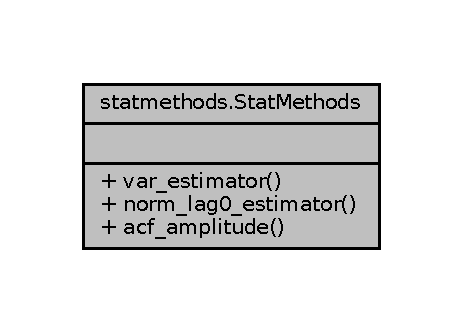
\includegraphics[width=222pt]{dc/d64/classstatmethods_1_1StatMethods__coll__graph}
\end{center}
\end{figure}
\subsection*{Public Member Functions}
\begin{DoxyCompactItemize}
\item 
def \hyperlink{classstatmethods_1_1StatMethods_ae9dd94cc0586ae5ea83ac6cf4a81cb69}{var\+\_\+estimator} (first\+\_\+moment, second\+\_\+moment, size)
\item 
def \hyperlink{classstatmethods_1_1StatMethods_a98bde45d59d8558c9b675b9f5dbd0922}{norm\+\_\+lag0\+\_\+estimator} (mean, variance)
\item 
def \hyperlink{classstatmethods_1_1StatMethods_a7ceddee9254bdb4e664b4d798d67f870}{acf\+\_\+amplitude} (norm\+\_\+acf)
\end{DoxyCompactItemize}


\subsection{Member Function Documentation}
\mbox{\Hypertarget{classstatmethods_1_1StatMethods_a7ceddee9254bdb4e664b4d798d67f870}\label{classstatmethods_1_1StatMethods_a7ceddee9254bdb4e664b4d798d67f870}} 
\index{statmethods\+::\+Stat\+Methods@{statmethods\+::\+Stat\+Methods}!acf\+\_\+amplitude@{acf\+\_\+amplitude}}
\index{acf\+\_\+amplitude@{acf\+\_\+amplitude}!statmethods\+::\+Stat\+Methods@{statmethods\+::\+Stat\+Methods}}
\subsubsection{\texorpdfstring{acf\+\_\+amplitude()}{acf\_amplitude()}}
{\footnotesize\ttfamily def statmethods.\+Stat\+Methods.\+acf\+\_\+amplitude (\begin{DoxyParamCaption}\item[{}]{norm\+\_\+acf }\end{DoxyParamCaption})}

\mbox{\Hypertarget{classstatmethods_1_1StatMethods_a98bde45d59d8558c9b675b9f5dbd0922}\label{classstatmethods_1_1StatMethods_a98bde45d59d8558c9b675b9f5dbd0922}} 
\index{statmethods\+::\+Stat\+Methods@{statmethods\+::\+Stat\+Methods}!norm\+\_\+lag0\+\_\+estimator@{norm\+\_\+lag0\+\_\+estimator}}
\index{norm\+\_\+lag0\+\_\+estimator@{norm\+\_\+lag0\+\_\+estimator}!statmethods\+::\+Stat\+Methods@{statmethods\+::\+Stat\+Methods}}
\subsubsection{\texorpdfstring{norm\+\_\+lag0\+\_\+estimator()}{norm\_lag0\_estimator()}}
{\footnotesize\ttfamily def statmethods.\+Stat\+Methods.\+norm\+\_\+lag0\+\_\+estimator (\begin{DoxyParamCaption}\item[{}]{mean,  }\item[{}]{variance }\end{DoxyParamCaption})}

\mbox{\Hypertarget{classstatmethods_1_1StatMethods_ae9dd94cc0586ae5ea83ac6cf4a81cb69}\label{classstatmethods_1_1StatMethods_ae9dd94cc0586ae5ea83ac6cf4a81cb69}} 
\index{statmethods\+::\+Stat\+Methods@{statmethods\+::\+Stat\+Methods}!var\+\_\+estimator@{var\+\_\+estimator}}
\index{var\+\_\+estimator@{var\+\_\+estimator}!statmethods\+::\+Stat\+Methods@{statmethods\+::\+Stat\+Methods}}
\subsubsection{\texorpdfstring{var\+\_\+estimator()}{var\_estimator()}}
{\footnotesize\ttfamily def statmethods.\+Stat\+Methods.\+var\+\_\+estimator (\begin{DoxyParamCaption}\item[{}]{first\+\_\+moment,  }\item[{}]{second\+\_\+moment,  }\item[{}]{size }\end{DoxyParamCaption})}



The documentation for this class was generated from the following file\+:\begin{DoxyCompactItemize}
\item 
code/pc\+\_\+app/\hyperlink{statmethods_8py}{statmethods.\+py}\end{DoxyCompactItemize}

\hypertarget{classdevice__mode_1_1StructParsar}{}\section{device\+\_\+mode.\+Struct\+Parsar Class Reference}
\label{classdevice__mode_1_1StructParsar}\index{device\+\_\+mode.\+Struct\+Parsar@{device\+\_\+mode.\+Struct\+Parsar}}
\subsection*{Public Member Functions}
\begin{DoxyCompactItemize}
\item 
def \hyperlink{classdevice__mode_1_1StructParsar_a3fd85c5d99b5bfc1e359d9457cc07df1}{\+\_\+\+\_\+init\+\_\+\+\_\+} (self, session\+\_\+name, parent\+\_\+dir, \hyperlink{classdevice__mode_1_1StructParsar_a54cc58295d8352d412afb79f32f1ac06}{config}, \hyperlink{classdevice__mode_1_1StructParsar_a0f1adb7dde59a293a12a4889e9b3880b}{add\+\_\+suffix}=False)
\item 
def \hyperlink{classdevice__mode_1_1StructParsar_a27f6ebed8dceb8e44d29294383288ea3}{fl\+\_\+structure} (self)
\item 
def \hyperlink{classdevice__mode_1_1StructParsar_ad08ea57819388138c2e94a43780b6da5}{get\+\_\+struct\+\_\+size} ()
\item 
def \hyperlink{classdevice__mode_1_1StructParsar_aa712e82c9d517f5dc900a2160087b544}{copy\+\_\+config\+\_\+to\+\_\+session} ()
\item 
def \hyperlink{classdevice__mode_1_1StructParsar_a4cdbf854c368e74051b505cca98ec41e}{set\+\_\+config} (\hyperlink{classdevice__mode_1_1StructParsar_a54cc58295d8352d412afb79f32f1ac06}{config})
\item 
def \hyperlink{classdevice__mode_1_1StructParsar_ae57ed24c72707985427085a6ba87087c}{generate\+\_\+data\+\_\+files} ()
\item 
def \hyperlink{classdevice__mode_1_1StructParsar_aa61ace2e8ff58899b980e083c442bd7c}{generate\+\_\+datasets} ()
\item 
def \hyperlink{classdevice__mode_1_1StructParsar_a0292edb37b72eb19e711d58f6fc2567f}{generate\+\_\+struct\+\_\+rep} ()
\item 
def \hyperlink{classdevice__mode_1_1StructParsar_a41a89941190ffef686890ed45110a086}{file\+\_\+name\+\_\+generator} (self, \hyperlink{classdevice__mode_1_1StructParsar_a937fe4559444433d8cff05910c16a4b6}{name})
\item 
def \hyperlink{classdevice__mode_1_1StructParsar_a87d7fedb8e4d87378eab71acc68dfb43}{create\+\_\+file} (self, \hyperlink{classdevice__mode_1_1StructParsar_a937fe4559444433d8cff05910c16a4b6}{name})
\item 
def \hyperlink{classdevice__mode_1_1StructParsar_afe15c55fc572e5fa0f02bf03188de789}{generate\+\_\+struct\+\_\+parsar} (self)
\end{DoxyCompactItemize}
\subsection*{Public Attributes}
\begin{DoxyCompactItemize}
\item 
\hyperlink{classdevice__mode_1_1StructParsar_a6f57d24a6006d990240bfcabfc06782f}{dstore}
\item 
\hyperlink{classdevice__mode_1_1StructParsar_acd42c1ec4385bc3acaa7a265df70d4be}{data}
\item 
\hyperlink{classdevice__mode_1_1StructParsar_a1e7769eb90fbb3821659d58b5607d17f}{root\+\_\+dir}
\item 
\hyperlink{classdevice__mode_1_1StructParsar_a937fe4559444433d8cff05910c16a4b6}{name}
\item 
\hyperlink{classdevice__mode_1_1StructParsar_a0f1adb7dde59a293a12a4889e9b3880b}{add\+\_\+suffix}
\item 
\hyperlink{classdevice__mode_1_1StructParsar_a54cc58295d8352d412afb79f32f1ac06}{config}
\item 
\hyperlink{classdevice__mode_1_1StructParsar_ad41412b88f13b25fc0dffcf5c62b4259}{mt\+\_\+param}
\end{DoxyCompactItemize}


\subsection{Constructor \& Destructor Documentation}
\mbox{\Hypertarget{classdevice__mode_1_1StructParsar_a3fd85c5d99b5bfc1e359d9457cc07df1}\label{classdevice__mode_1_1StructParsar_a3fd85c5d99b5bfc1e359d9457cc07df1}} 
\index{device\+\_\+mode\+::\+Struct\+Parsar@{device\+\_\+mode\+::\+Struct\+Parsar}!\+\_\+\+\_\+init\+\_\+\+\_\+@{\+\_\+\+\_\+init\+\_\+\+\_\+}}
\index{\+\_\+\+\_\+init\+\_\+\+\_\+@{\+\_\+\+\_\+init\+\_\+\+\_\+}!device\+\_\+mode\+::\+Struct\+Parsar@{device\+\_\+mode\+::\+Struct\+Parsar}}
\subsubsection{\texorpdfstring{\+\_\+\+\_\+init\+\_\+\+\_\+()}{\_\_init\_\_()}}
{\footnotesize\ttfamily def device\+\_\+mode.\+Struct\+Parsar.\+\_\+\+\_\+init\+\_\+\+\_\+ (\begin{DoxyParamCaption}\item[{}]{self,  }\item[{}]{session\+\_\+name,  }\item[{}]{parent\+\_\+dir,  }\item[{}]{config,  }\item[{}]{add\+\_\+suffix = {\ttfamily False} }\end{DoxyParamCaption})}



\subsection{Member Function Documentation}
\mbox{\Hypertarget{classdevice__mode_1_1StructParsar_aa712e82c9d517f5dc900a2160087b544}\label{classdevice__mode_1_1StructParsar_aa712e82c9d517f5dc900a2160087b544}} 
\index{device\+\_\+mode\+::\+Struct\+Parsar@{device\+\_\+mode\+::\+Struct\+Parsar}!copy\+\_\+config\+\_\+to\+\_\+session@{copy\+\_\+config\+\_\+to\+\_\+session}}
\index{copy\+\_\+config\+\_\+to\+\_\+session@{copy\+\_\+config\+\_\+to\+\_\+session}!device\+\_\+mode\+::\+Struct\+Parsar@{device\+\_\+mode\+::\+Struct\+Parsar}}
\subsubsection{\texorpdfstring{copy\+\_\+config\+\_\+to\+\_\+session()}{copy\_config\_to\_session()}}
{\footnotesize\ttfamily def device\+\_\+mode.\+Struct\+Parsar.\+copy\+\_\+config\+\_\+to\+\_\+session (\begin{DoxyParamCaption}{ }\end{DoxyParamCaption})}

\begin{DoxyVerb}Copies the current configuration file to the session directory.
\end{DoxyVerb}
 \mbox{\Hypertarget{classdevice__mode_1_1StructParsar_a87d7fedb8e4d87378eab71acc68dfb43}\label{classdevice__mode_1_1StructParsar_a87d7fedb8e4d87378eab71acc68dfb43}} 
\index{device\+\_\+mode\+::\+Struct\+Parsar@{device\+\_\+mode\+::\+Struct\+Parsar}!create\+\_\+file@{create\+\_\+file}}
\index{create\+\_\+file@{create\+\_\+file}!device\+\_\+mode\+::\+Struct\+Parsar@{device\+\_\+mode\+::\+Struct\+Parsar}}
\subsubsection{\texorpdfstring{create\+\_\+file()}{create\_file()}}
{\footnotesize\ttfamily def device\+\_\+mode.\+Struct\+Parsar.\+create\+\_\+file (\begin{DoxyParamCaption}\item[{}]{self,  }\item[{}]{name }\end{DoxyParamCaption})}

\begin{DoxyVerb}Creates a file with a given name (name should be unique or it would override
the past instance) and saves a reference to the `open_files` dictionary.
\end{DoxyVerb}
 \mbox{\Hypertarget{classdevice__mode_1_1StructParsar_a41a89941190ffef686890ed45110a086}\label{classdevice__mode_1_1StructParsar_a41a89941190ffef686890ed45110a086}} 
\index{device\+\_\+mode\+::\+Struct\+Parsar@{device\+\_\+mode\+::\+Struct\+Parsar}!file\+\_\+name\+\_\+generator@{file\+\_\+name\+\_\+generator}}
\index{file\+\_\+name\+\_\+generator@{file\+\_\+name\+\_\+generator}!device\+\_\+mode\+::\+Struct\+Parsar@{device\+\_\+mode\+::\+Struct\+Parsar}}
\subsubsection{\texorpdfstring{file\+\_\+name\+\_\+generator()}{file\_name\_generator()}}
{\footnotesize\ttfamily def device\+\_\+mode.\+Struct\+Parsar.\+file\+\_\+name\+\_\+generator (\begin{DoxyParamCaption}\item[{}]{self,  }\item[{}]{name }\end{DoxyParamCaption})}

\begin{DoxyVerb}Generates the file paths for the data files.
\end{DoxyVerb}
 \mbox{\Hypertarget{classdevice__mode_1_1StructParsar_a27f6ebed8dceb8e44d29294383288ea3}\label{classdevice__mode_1_1StructParsar_a27f6ebed8dceb8e44d29294383288ea3}} 
\index{device\+\_\+mode\+::\+Struct\+Parsar@{device\+\_\+mode\+::\+Struct\+Parsar}!fl\+\_\+structure@{fl\+\_\+structure}}
\index{fl\+\_\+structure@{fl\+\_\+structure}!device\+\_\+mode\+::\+Struct\+Parsar@{device\+\_\+mode\+::\+Struct\+Parsar}}
\subsubsection{\texorpdfstring{fl\+\_\+structure()}{fl\_structure()}}
{\footnotesize\ttfamily def device\+\_\+mode.\+Struct\+Parsar.\+fl\+\_\+structure (\begin{DoxyParamCaption}\item[{}]{self }\end{DoxyParamCaption})}

\begin{DoxyVerb}Layout of feature line structure.
\end{DoxyVerb}
 \mbox{\Hypertarget{classdevice__mode_1_1StructParsar_ae57ed24c72707985427085a6ba87087c}\label{classdevice__mode_1_1StructParsar_ae57ed24c72707985427085a6ba87087c}} 
\index{device\+\_\+mode\+::\+Struct\+Parsar@{device\+\_\+mode\+::\+Struct\+Parsar}!generate\+\_\+data\+\_\+files@{generate\+\_\+data\+\_\+files}}
\index{generate\+\_\+data\+\_\+files@{generate\+\_\+data\+\_\+files}!device\+\_\+mode\+::\+Struct\+Parsar@{device\+\_\+mode\+::\+Struct\+Parsar}}
\subsubsection{\texorpdfstring{generate\+\_\+data\+\_\+files()}{generate\_data\_files()}}
{\footnotesize\ttfamily def device\+\_\+mode.\+Struct\+Parsar.\+generate\+\_\+data\+\_\+files (\begin{DoxyParamCaption}{ }\end{DoxyParamCaption})}

\begin{DoxyVerb}Generates the relavent data files for the feature line.
\end{DoxyVerb}
 \mbox{\Hypertarget{classdevice__mode_1_1StructParsar_aa61ace2e8ff58899b980e083c442bd7c}\label{classdevice__mode_1_1StructParsar_aa61ace2e8ff58899b980e083c442bd7c}} 
\index{device\+\_\+mode\+::\+Struct\+Parsar@{device\+\_\+mode\+::\+Struct\+Parsar}!generate\+\_\+datasets@{generate\+\_\+datasets}}
\index{generate\+\_\+datasets@{generate\+\_\+datasets}!device\+\_\+mode\+::\+Struct\+Parsar@{device\+\_\+mode\+::\+Struct\+Parsar}}
\subsubsection{\texorpdfstring{generate\+\_\+datasets()}{generate\_datasets()}}
{\footnotesize\ttfamily def device\+\_\+mode.\+Struct\+Parsar.\+generate\+\_\+datasets (\begin{DoxyParamCaption}{ }\end{DoxyParamCaption})}

\begin{DoxyVerb}Populates the `data` dict with the required data sets → arrays, lists, or deques as required.
\end{DoxyVerb}
 \mbox{\Hypertarget{classdevice__mode_1_1StructParsar_afe15c55fc572e5fa0f02bf03188de789}\label{classdevice__mode_1_1StructParsar_afe15c55fc572e5fa0f02bf03188de789}} 
\index{device\+\_\+mode\+::\+Struct\+Parsar@{device\+\_\+mode\+::\+Struct\+Parsar}!generate\+\_\+struct\+\_\+parsar@{generate\+\_\+struct\+\_\+parsar}}
\index{generate\+\_\+struct\+\_\+parsar@{generate\+\_\+struct\+\_\+parsar}!device\+\_\+mode\+::\+Struct\+Parsar@{device\+\_\+mode\+::\+Struct\+Parsar}}
\subsubsection{\texorpdfstring{generate\+\_\+struct\+\_\+parsar()}{generate\_struct\_parsar()}}
{\footnotesize\ttfamily def device\+\_\+mode.\+Struct\+Parsar.\+generate\+\_\+struct\+\_\+parsar (\begin{DoxyParamCaption}\item[{}]{self }\end{DoxyParamCaption})}

\mbox{\Hypertarget{classdevice__mode_1_1StructParsar_a0292edb37b72eb19e711d58f6fc2567f}\label{classdevice__mode_1_1StructParsar_a0292edb37b72eb19e711d58f6fc2567f}} 
\index{device\+\_\+mode\+::\+Struct\+Parsar@{device\+\_\+mode\+::\+Struct\+Parsar}!generate\+\_\+struct\+\_\+rep@{generate\+\_\+struct\+\_\+rep}}
\index{generate\+\_\+struct\+\_\+rep@{generate\+\_\+struct\+\_\+rep}!device\+\_\+mode\+::\+Struct\+Parsar@{device\+\_\+mode\+::\+Struct\+Parsar}}
\subsubsection{\texorpdfstring{generate\+\_\+struct\+\_\+rep()}{generate\_struct\_rep()}}
{\footnotesize\ttfamily def device\+\_\+mode.\+Struct\+Parsar.\+generate\+\_\+struct\+\_\+rep (\begin{DoxyParamCaption}{ }\end{DoxyParamCaption})}

\mbox{\Hypertarget{classdevice__mode_1_1StructParsar_ad08ea57819388138c2e94a43780b6da5}\label{classdevice__mode_1_1StructParsar_ad08ea57819388138c2e94a43780b6da5}} 
\index{device\+\_\+mode\+::\+Struct\+Parsar@{device\+\_\+mode\+::\+Struct\+Parsar}!get\+\_\+struct\+\_\+size@{get\+\_\+struct\+\_\+size}}
\index{get\+\_\+struct\+\_\+size@{get\+\_\+struct\+\_\+size}!device\+\_\+mode\+::\+Struct\+Parsar@{device\+\_\+mode\+::\+Struct\+Parsar}}
\subsubsection{\texorpdfstring{get\+\_\+struct\+\_\+size()}{get\_struct\_size()}}
{\footnotesize\ttfamily def device\+\_\+mode.\+Struct\+Parsar.\+get\+\_\+struct\+\_\+size (\begin{DoxyParamCaption}{ }\end{DoxyParamCaption})}

\begin{DoxyVerb}Calculates and returns the size of the receiving struct.
\end{DoxyVerb}
 \mbox{\Hypertarget{classdevice__mode_1_1StructParsar_a4cdbf854c368e74051b505cca98ec41e}\label{classdevice__mode_1_1StructParsar_a4cdbf854c368e74051b505cca98ec41e}} 
\index{device\+\_\+mode\+::\+Struct\+Parsar@{device\+\_\+mode\+::\+Struct\+Parsar}!set\+\_\+config@{set\+\_\+config}}
\index{set\+\_\+config@{set\+\_\+config}!device\+\_\+mode\+::\+Struct\+Parsar@{device\+\_\+mode\+::\+Struct\+Parsar}}
\subsubsection{\texorpdfstring{set\+\_\+config()}{set\_config()}}
{\footnotesize\ttfamily def device\+\_\+mode.\+Struct\+Parsar.\+set\+\_\+config (\begin{DoxyParamCaption}\item[{}]{config }\end{DoxyParamCaption})}

\begin{DoxyVerb}Creates a local store of configuration.
Accepts both a dictionary or a config file path.
\end{DoxyVerb}
 

\subsection{Member Data Documentation}
\mbox{\Hypertarget{classdevice__mode_1_1StructParsar_a0f1adb7dde59a293a12a4889e9b3880b}\label{classdevice__mode_1_1StructParsar_a0f1adb7dde59a293a12a4889e9b3880b}} 
\index{device\+\_\+mode\+::\+Struct\+Parsar@{device\+\_\+mode\+::\+Struct\+Parsar}!add\+\_\+suffix@{add\+\_\+suffix}}
\index{add\+\_\+suffix@{add\+\_\+suffix}!device\+\_\+mode\+::\+Struct\+Parsar@{device\+\_\+mode\+::\+Struct\+Parsar}}
\subsubsection{\texorpdfstring{add\+\_\+suffix}{add\_suffix}}
{\footnotesize\ttfamily device\+\_\+mode.\+Struct\+Parsar.\+add\+\_\+suffix}

\mbox{\Hypertarget{classdevice__mode_1_1StructParsar_a54cc58295d8352d412afb79f32f1ac06}\label{classdevice__mode_1_1StructParsar_a54cc58295d8352d412afb79f32f1ac06}} 
\index{device\+\_\+mode\+::\+Struct\+Parsar@{device\+\_\+mode\+::\+Struct\+Parsar}!config@{config}}
\index{config@{config}!device\+\_\+mode\+::\+Struct\+Parsar@{device\+\_\+mode\+::\+Struct\+Parsar}}
\subsubsection{\texorpdfstring{config}{config}}
{\footnotesize\ttfamily device\+\_\+mode.\+Struct\+Parsar.\+config}

\begin{DoxyVerb}Creates a local store of configuration.
Accepts both a dictionary or a config file path.
\end{DoxyVerb}
 \mbox{\Hypertarget{classdevice__mode_1_1StructParsar_acd42c1ec4385bc3acaa7a265df70d4be}\label{classdevice__mode_1_1StructParsar_acd42c1ec4385bc3acaa7a265df70d4be}} 
\index{device\+\_\+mode\+::\+Struct\+Parsar@{device\+\_\+mode\+::\+Struct\+Parsar}!data@{data}}
\index{data@{data}!device\+\_\+mode\+::\+Struct\+Parsar@{device\+\_\+mode\+::\+Struct\+Parsar}}
\subsubsection{\texorpdfstring{data}{data}}
{\footnotesize\ttfamily device\+\_\+mode.\+Struct\+Parsar.\+data}

\mbox{\Hypertarget{classdevice__mode_1_1StructParsar_a6f57d24a6006d990240bfcabfc06782f}\label{classdevice__mode_1_1StructParsar_a6f57d24a6006d990240bfcabfc06782f}} 
\index{device\+\_\+mode\+::\+Struct\+Parsar@{device\+\_\+mode\+::\+Struct\+Parsar}!dstore@{dstore}}
\index{dstore@{dstore}!device\+\_\+mode\+::\+Struct\+Parsar@{device\+\_\+mode\+::\+Struct\+Parsar}}
\subsubsection{\texorpdfstring{dstore}{dstore}}
{\footnotesize\ttfamily device\+\_\+mode.\+Struct\+Parsar.\+dstore}

\mbox{\Hypertarget{classdevice__mode_1_1StructParsar_ad41412b88f13b25fc0dffcf5c62b4259}\label{classdevice__mode_1_1StructParsar_ad41412b88f13b25fc0dffcf5c62b4259}} 
\index{device\+\_\+mode\+::\+Struct\+Parsar@{device\+\_\+mode\+::\+Struct\+Parsar}!mt\+\_\+param@{mt\+\_\+param}}
\index{mt\+\_\+param@{mt\+\_\+param}!device\+\_\+mode\+::\+Struct\+Parsar@{device\+\_\+mode\+::\+Struct\+Parsar}}
\subsubsection{\texorpdfstring{mt\+\_\+param}{mt\_param}}
{\footnotesize\ttfamily device\+\_\+mode.\+Struct\+Parsar.\+mt\+\_\+param}

\begin{DoxyVerb}Populates the `data` dict with the required data sets → arrays, lists, or deques as required.
\end{DoxyVerb}
\begin{DoxyVerb}Constructs a deque and populates it to zero to prevent arithmetic errors, etc.
\end{DoxyVerb}
 \mbox{\Hypertarget{classdevice__mode_1_1StructParsar_a937fe4559444433d8cff05910c16a4b6}\label{classdevice__mode_1_1StructParsar_a937fe4559444433d8cff05910c16a4b6}} 
\index{device\+\_\+mode\+::\+Struct\+Parsar@{device\+\_\+mode\+::\+Struct\+Parsar}!name@{name}}
\index{name@{name}!device\+\_\+mode\+::\+Struct\+Parsar@{device\+\_\+mode\+::\+Struct\+Parsar}}
\subsubsection{\texorpdfstring{name}{name}}
{\footnotesize\ttfamily device\+\_\+mode.\+Struct\+Parsar.\+name}

\mbox{\Hypertarget{classdevice__mode_1_1StructParsar_a1e7769eb90fbb3821659d58b5607d17f}\label{classdevice__mode_1_1StructParsar_a1e7769eb90fbb3821659d58b5607d17f}} 
\index{device\+\_\+mode\+::\+Struct\+Parsar@{device\+\_\+mode\+::\+Struct\+Parsar}!root\+\_\+dir@{root\+\_\+dir}}
\index{root\+\_\+dir@{root\+\_\+dir}!device\+\_\+mode\+::\+Struct\+Parsar@{device\+\_\+mode\+::\+Struct\+Parsar}}
\subsubsection{\texorpdfstring{root\+\_\+dir}{root\_dir}}
{\footnotesize\ttfamily device\+\_\+mode.\+Struct\+Parsar.\+root\+\_\+dir}



The documentation for this class was generated from the following file\+:\begin{DoxyCompactItemize}
\item 
code/pc\+\_\+app/\hyperlink{device__mode_8py}{device\+\_\+mode.\+py}\end{DoxyCompactItemize}

\hypertarget{classTMR1Controller}{}\section{T\+M\+R1\+Controller Class Reference}
\label{classTMR1Controller}\index{T\+M\+R1\+Controller@{T\+M\+R1\+Controller}}


Templated interface for Quad Timer 1 channels for Gate Counting. The module uses the macro {\ttfamily \+\_\+\+T\+M\+R1\+\_\+\+C\+O\+N\+T\+R\+O\+L\+L\+E\+R\+\_\+\+C\+H\+\_\+} to identify the main channel and then assigns the next channel\textquotesingle{}s ({\itshape T\+M\+R1\+\_\+\+C\+O\+N\+T\+R\+O\+L\+L\+E\+R\+\_\+\+CH} + 1) external pin to the {\itshape T\+M\+R1\+\_\+\+C\+O\+N\+T\+R\+O\+L\+L\+E\+R\+\_\+\+CH} as the \char`\"{}\+Capture Pin\char`\"{} or the \char`\"{}\+Secondary Count Source\char`\"{}.  




{\ttfamily \#include $<$qtmr1.\+hpp$>$}

\subsection*{Public Member Functions}
\begin{DoxyCompactItemize}
\item 
\hyperlink{classTMR1Controller_aebc677e795f673c6520d5a03eb6aa4f2}{T\+M\+R1\+Controller} ()
\begin{DoxyCompactList}\small\item\em Singleton template. \end{DoxyCompactList}\item 
void \hyperlink{classTMR1Controller_a67bc04f0648176a681f6ac01ea483db9}{start} () \hyperlink{utilities_8hpp_a103d5b3998e0dd804213c8f30a094f4d}{\+\_\+\+\_\+attribute\+\_\+\+\_\+}((\hyperlink{classTMR1Controller_adce8e8a496510485a88ccc5b88595672}{always\+\_\+inline}))
\begin{DoxyCompactList}\small\item\em Starts up-\/counting from the set counter value. \end{DoxyCompactList}\item 
void \hyperlink{classTMR1Controller_afcb0ea27107bfbe50b9dcbd54207dd00}{stop} () \hyperlink{utilities_8hpp_a103d5b3998e0dd804213c8f30a094f4d}{\+\_\+\+\_\+attribute\+\_\+\+\_\+}((\hyperlink{classTMR1Controller_adce8e8a496510485a88ccc5b88595672}{always\+\_\+inline}))
\begin{DoxyCompactList}\small\item\em Stops counting and freezes the current counter value. \end{DoxyCompactList}\item 
void \hyperlink{classTMR1Controller_adf3746ffd24c5b55abff4fa18e05f6b3}{reset} () \hyperlink{utilities_8hpp_a103d5b3998e0dd804213c8f30a094f4d}{\+\_\+\+\_\+attribute\+\_\+\+\_\+}((\hyperlink{classTMR1Controller_adce8e8a496510485a88ccc5b88595672}{always\+\_\+inline}))
\begin{DoxyCompactList}\small\item\em Resets the counter to zero. It also cleares the capture register and unsets the Input Edge Flag. \end{DoxyCompactList}\item 
\hyperlink{types_8hpp_ac89ac912f524b3e3fa3720ea55fec966}{counter\+\_\+t} \hyperlink{classTMR1Controller_a3d07eed72365e7a7b44fadefb23b9ba6}{get\+\_\+capture\+\_\+val} () \hyperlink{utilities_8hpp_a103d5b3998e0dd804213c8f30a094f4d}{\+\_\+\+\_\+attribute\+\_\+\+\_\+}((\hyperlink{classTMR1Controller_adce8e8a496510485a88ccc5b88595672}{always\+\_\+inline}))
\begin{DoxyCompactList}\small\item\em Reads and returns the Capture Register. \end{DoxyCompactList}\item 
\hyperlink{types_8hpp_ac89ac912f524b3e3fa3720ea55fec966}{counter\+\_\+t} \hyperlink{classTMR1Controller_a34042b5a735d4f8fd40fa36135bdec8c}{get\+\_\+capture\+\_\+double\+\_\+range} () \hyperlink{utilities_8hpp_a103d5b3998e0dd804213c8f30a094f4d}{\+\_\+\+\_\+attribute\+\_\+\+\_\+}((flatten
\begin{DoxyCompactList}\small\item\em Returns a value that has range (2 X 2$\ast$$\ast$n -\/ 1). This is done by checking the overflow flag. \end{DoxyCompactList}\item 
bool \hyperlink{classTMR1Controller_a06052b4a881156be3c7a4b6495d8ca11}{is\+\_\+overflow} () \hyperlink{utilities_8hpp_a103d5b3998e0dd804213c8f30a094f4d}{\+\_\+\+\_\+attribute\+\_\+\+\_\+}((\hyperlink{classTMR1Controller_adce8e8a496510485a88ccc5b88595672}{always\+\_\+inline}))
\begin{DoxyCompactList}\small\item\em Returns the overflow status of the Counter. Reads the T\+OF -\/ Timer Overflow Flag. \end{DoxyCompactList}\item 
void \hyperlink{classTMR1Controller_aa59afefa545098e53cb2e0560142526c}{clear\+\_\+input\+\_\+edge\+\_\+flag} () \hyperlink{utilities_8hpp_a103d5b3998e0dd804213c8f30a094f4d}{\+\_\+\+\_\+attribute\+\_\+\+\_\+}((\hyperlink{classTMR1Controller_adce8e8a496510485a88ccc5b88595672}{always\+\_\+inline}))
\item 
void \hyperlink{classTMR1Controller_a7117e12d0cb8ec32aa6552fe541023da}{clear\+\_\+overflow\+\_\+flag} () \hyperlink{utilities_8hpp_a103d5b3998e0dd804213c8f30a094f4d}{\+\_\+\+\_\+attribute\+\_\+\+\_\+}((\hyperlink{classTMR1Controller_adce8e8a496510485a88ccc5b88595672}{always\+\_\+inline}))
\item 
int \hyperlink{classTMR1Controller_a084c153e1a888f72456c54b29e3fa957}{get\+\_\+ttl\+\_\+input\+\_\+pin} () \hyperlink{utilities_8hpp_a103d5b3998e0dd804213c8f30a094f4d}{\+\_\+\+\_\+attribute\+\_\+\+\_\+}((\hyperlink{classTMR1Controller_adce8e8a496510485a88ccc5b88595672}{always\+\_\+inline}))
\begin{DoxyCompactList}\small\item\em Returns the pin number on which the T\+TL input must be connected. \end{DoxyCompactList}\item 
void \hyperlink{classTMR1Controller_af92315e340766e3857eb6a20e7cab673}{init} () \hyperlink{utilities_8hpp_a103d5b3998e0dd804213c8f30a094f4d}{\+\_\+\+\_\+attribute\+\_\+\+\_\+}((\hyperlink{classTMR1Controller_adce8e8a496510485a88ccc5b88595672}{always\+\_\+inline}))
\item 
void \hyperlink{classTMR1Controller_a1c5d358760aa98641333f63c7bcacd3a}{init\+\_\+pins} () \hyperlink{utilities_8hpp_a103d5b3998e0dd804213c8f30a094f4d}{\+\_\+\+\_\+attribute\+\_\+\+\_\+}((\hyperlink{classTMR1Controller_adce8e8a496510485a88ccc5b88595672}{always\+\_\+inline}))
\begin{DoxyCompactList}\small\item\em Sets the Primary and Secondary inputs for Capture Mode, routed through X\+B\+AR.  X\+B\+AR and I\+O\+M\+UX input selections → I\+O\+M\+U\+X\+C\+\_\+\+G\+P\+R\+\_\+\+G\+P\+R6 Manual Page 347. \end{DoxyCompactList}\item 
unsigned int \hyperlink{classTMR1Controller_a5b2f74d17a84db6a9c2957b75d79ab98}{get\+\_\+xbar\+\_\+out\+\_\+pin} () \hyperlink{utilities_8hpp_a103d5b3998e0dd804213c8f30a094f4d}{\+\_\+\+\_\+attribute\+\_\+\+\_\+}((\hyperlink{classTMR1Controller_adce8e8a496510485a88ccc5b88595672}{always\+\_\+inline}))
\begin{DoxyCompactList}\small\item\em Returns the corresponding X\+B\+AR Output Pin to use for routing the Capture Signal.  Manual Page 70. \end{DoxyCompactList}\end{DoxyCompactItemize}
\subsection*{Static Public Member Functions}
\begin{DoxyCompactItemize}
\item 
static void \hyperlink{classTMR1Controller_aa00df5e2d591a36b1049275c9a293c51}{timers\+\_\+freeze} () \hyperlink{utilities_8hpp_a103d5b3998e0dd804213c8f30a094f4d}{\+\_\+\+\_\+attribute\+\_\+\+\_\+}((\hyperlink{classTMR1Controller_adce8e8a496510485a88ccc5b88595672}{always\+\_\+inline}))
\begin{DoxyCompactList}\small\item\em Reset Counter and output flags.  Manual Page 332. \end{DoxyCompactList}\item 
static void \hyperlink{classTMR1Controller_acb383aa5321f552f018e4e217e2211f4}{timers\+\_\+anti\+\_\+freeze} () \hyperlink{utilities_8hpp_a103d5b3998e0dd804213c8f30a094f4d}{\+\_\+\+\_\+attribute\+\_\+\+\_\+}((\hyperlink{classTMR1Controller_adce8e8a496510485a88ccc5b88595672}{always\+\_\+inline}))
\begin{DoxyCompactList}\small\item\em Enable counting normally.  Manual Page 332. \end{DoxyCompactList}\end{DoxyCompactItemize}
\subsection*{Public Attributes}
\begin{DoxyCompactItemize}
\item 
\hyperlink{types_8hpp_ac89ac912f524b3e3fa3720ea55fec966}{counter\+\_\+t} \hyperlink{classTMR1Controller_adce8e8a496510485a88ccc5b88595672}{always\+\_\+inline}
\end{DoxyCompactItemize}
\subsection*{Static Private Attributes}
\begin{DoxyCompactItemize}
\item 
static constexpr bool \hyperlink{classTMR1Controller_a532b729ca9a7c28e5f4d221f80487241}{Singleton\+\_\+flag} = false
\end{DoxyCompactItemize}


\subsection{Detailed Description}
Templated interface for Quad Timer 1 channels for Gate Counting. The module uses the macro {\ttfamily \+\_\+\+T\+M\+R1\+\_\+\+C\+O\+N\+T\+R\+O\+L\+L\+E\+R\+\_\+\+C\+H\+\_\+} to identify the main channel and then assigns the next channel\textquotesingle{}s ({\itshape T\+M\+R1\+\_\+\+C\+O\+N\+T\+R\+O\+L\+L\+E\+R\+\_\+\+CH} + 1) external pin to the {\itshape T\+M\+R1\+\_\+\+C\+O\+N\+T\+R\+O\+L\+L\+E\+R\+\_\+\+CH} as the \char`\"{}\+Capture Pin\char`\"{} or the \char`\"{}\+Secondary Count Source\char`\"{}. 

\subsection{Constructor \& Destructor Documentation}
\mbox{\Hypertarget{classTMR1Controller_aebc677e795f673c6520d5a03eb6aa4f2}\label{classTMR1Controller_aebc677e795f673c6520d5a03eb6aa4f2}} 
\index{T\+M\+R1\+Controller@{T\+M\+R1\+Controller}!T\+M\+R1\+Controller@{T\+M\+R1\+Controller}}
\index{T\+M\+R1\+Controller@{T\+M\+R1\+Controller}!T\+M\+R1\+Controller@{T\+M\+R1\+Controller}}
\subsubsection{\texorpdfstring{T\+M\+R1\+Controller()}{TMR1Controller()}}
{\footnotesize\ttfamily T\+M\+R1\+Controller\+::\+T\+M\+R1\+Controller (\begin{DoxyParamCaption}{ }\end{DoxyParamCaption})\hspace{0.3cm}{\ttfamily [inline]}}



Singleton template. 

Default Constructor that assers if the user constructed object with a valid {\itshape T\+M\+R1\+\_\+\+C\+O\+N\+T\+R\+O\+L\+L\+E\+R\+\_\+\+CH}, and asserts a singleton template. 

\subsection{Member Function Documentation}
\mbox{\Hypertarget{classTMR1Controller_aa59afefa545098e53cb2e0560142526c}\label{classTMR1Controller_aa59afefa545098e53cb2e0560142526c}} 
\index{T\+M\+R1\+Controller@{T\+M\+R1\+Controller}!clear\+\_\+input\+\_\+edge\+\_\+flag@{clear\+\_\+input\+\_\+edge\+\_\+flag}}
\index{clear\+\_\+input\+\_\+edge\+\_\+flag@{clear\+\_\+input\+\_\+edge\+\_\+flag}!T\+M\+R1\+Controller@{T\+M\+R1\+Controller}}
\subsubsection{\texorpdfstring{clear\+\_\+input\+\_\+edge\+\_\+flag()}{clear\_input\_edge\_flag()}}
{\footnotesize\ttfamily void T\+M\+R1\+Controller\+::clear\+\_\+input\+\_\+edge\+\_\+flag (\begin{DoxyParamCaption}{ }\end{DoxyParamCaption})\hspace{0.3cm}{\ttfamily [inline]}}

\mbox{\Hypertarget{classTMR1Controller_a7117e12d0cb8ec32aa6552fe541023da}\label{classTMR1Controller_a7117e12d0cb8ec32aa6552fe541023da}} 
\index{T\+M\+R1\+Controller@{T\+M\+R1\+Controller}!clear\+\_\+overflow\+\_\+flag@{clear\+\_\+overflow\+\_\+flag}}
\index{clear\+\_\+overflow\+\_\+flag@{clear\+\_\+overflow\+\_\+flag}!T\+M\+R1\+Controller@{T\+M\+R1\+Controller}}
\subsubsection{\texorpdfstring{clear\+\_\+overflow\+\_\+flag()}{clear\_overflow\_flag()}}
{\footnotesize\ttfamily void T\+M\+R1\+Controller\+::clear\+\_\+overflow\+\_\+flag (\begin{DoxyParamCaption}{ }\end{DoxyParamCaption})\hspace{0.3cm}{\ttfamily [inline]}}

\mbox{\Hypertarget{classTMR1Controller_a34042b5a735d4f8fd40fa36135bdec8c}\label{classTMR1Controller_a34042b5a735d4f8fd40fa36135bdec8c}} 
\index{T\+M\+R1\+Controller@{T\+M\+R1\+Controller}!get\+\_\+capture\+\_\+double\+\_\+range@{get\+\_\+capture\+\_\+double\+\_\+range}}
\index{get\+\_\+capture\+\_\+double\+\_\+range@{get\+\_\+capture\+\_\+double\+\_\+range}!T\+M\+R1\+Controller@{T\+M\+R1\+Controller}}
\subsubsection{\texorpdfstring{get\+\_\+capture\+\_\+double\+\_\+range()}{get\_capture\_double\_range()}}
{\footnotesize\ttfamily \hyperlink{types_8hpp_ac89ac912f524b3e3fa3720ea55fec966}{counter\+\_\+t} T\+M\+R1\+Controller\+::get\+\_\+capture\+\_\+double\+\_\+range (\begin{DoxyParamCaption}{ }\end{DoxyParamCaption})}



Returns a value that has range (2 X 2$\ast$$\ast$n -\/ 1). This is done by checking the overflow flag. 

\mbox{\Hypertarget{classTMR1Controller_a3d07eed72365e7a7b44fadefb23b9ba6}\label{classTMR1Controller_a3d07eed72365e7a7b44fadefb23b9ba6}} 
\index{T\+M\+R1\+Controller@{T\+M\+R1\+Controller}!get\+\_\+capture\+\_\+val@{get\+\_\+capture\+\_\+val}}
\index{get\+\_\+capture\+\_\+val@{get\+\_\+capture\+\_\+val}!T\+M\+R1\+Controller@{T\+M\+R1\+Controller}}
\subsubsection{\texorpdfstring{get\+\_\+capture\+\_\+val()}{get\_capture\_val()}}
{\footnotesize\ttfamily \hyperlink{types_8hpp_ac89ac912f524b3e3fa3720ea55fec966}{counter\+\_\+t} T\+M\+R1\+Controller\+::get\+\_\+capture\+\_\+val (\begin{DoxyParamCaption}{ }\end{DoxyParamCaption})\hspace{0.3cm}{\ttfamily [inline]}}



Reads and returns the Capture Register. 

\mbox{\Hypertarget{classTMR1Controller_a084c153e1a888f72456c54b29e3fa957}\label{classTMR1Controller_a084c153e1a888f72456c54b29e3fa957}} 
\index{T\+M\+R1\+Controller@{T\+M\+R1\+Controller}!get\+\_\+ttl\+\_\+input\+\_\+pin@{get\+\_\+ttl\+\_\+input\+\_\+pin}}
\index{get\+\_\+ttl\+\_\+input\+\_\+pin@{get\+\_\+ttl\+\_\+input\+\_\+pin}!T\+M\+R1\+Controller@{T\+M\+R1\+Controller}}
\subsubsection{\texorpdfstring{get\+\_\+ttl\+\_\+input\+\_\+pin()}{get\_ttl\_input\_pin()}}
{\footnotesize\ttfamily int T\+M\+R1\+Controller\+::get\+\_\+ttl\+\_\+input\+\_\+pin (\begin{DoxyParamCaption}{ }\end{DoxyParamCaption})\hspace{0.3cm}{\ttfamily [inline]}}



Returns the pin number on which the T\+TL input must be connected. 

\begin{DoxyAttention}{Attention}
This function does not configure the pin or assign it to the Q\+T\+MR module. For that T\+M\+R1\+Controller\+::init\+\_\+pin() must be called. 
\end{DoxyAttention}
\mbox{\Hypertarget{classTMR1Controller_a5b2f74d17a84db6a9c2957b75d79ab98}\label{classTMR1Controller_a5b2f74d17a84db6a9c2957b75d79ab98}} 
\index{T\+M\+R1\+Controller@{T\+M\+R1\+Controller}!get\+\_\+xbar\+\_\+out\+\_\+pin@{get\+\_\+xbar\+\_\+out\+\_\+pin}}
\index{get\+\_\+xbar\+\_\+out\+\_\+pin@{get\+\_\+xbar\+\_\+out\+\_\+pin}!T\+M\+R1\+Controller@{T\+M\+R1\+Controller}}
\subsubsection{\texorpdfstring{get\+\_\+xbar\+\_\+out\+\_\+pin()}{get\_xbar\_out\_pin()}}
{\footnotesize\ttfamily unsigned int T\+M\+R1\+Controller\+::get\+\_\+xbar\+\_\+out\+\_\+pin (\begin{DoxyParamCaption}{ }\end{DoxyParamCaption})\hspace{0.3cm}{\ttfamily [inline]}}



Returns the corresponding X\+B\+AR Output Pin to use for routing the Capture Signal.  Manual Page 70. 

\mbox{\Hypertarget{classTMR1Controller_af92315e340766e3857eb6a20e7cab673}\label{classTMR1Controller_af92315e340766e3857eb6a20e7cab673}} 
\index{T\+M\+R1\+Controller@{T\+M\+R1\+Controller}!init@{init}}
\index{init@{init}!T\+M\+R1\+Controller@{T\+M\+R1\+Controller}}
\subsubsection{\texorpdfstring{init()}{init()}}
{\footnotesize\ttfamily void T\+M\+R1\+Controller\+::init (\begin{DoxyParamCaption}{ }\end{DoxyParamCaption})\hspace{0.3cm}{\ttfamily [inline]}}

\mbox{\Hypertarget{classTMR1Controller_a1c5d358760aa98641333f63c7bcacd3a}\label{classTMR1Controller_a1c5d358760aa98641333f63c7bcacd3a}} 
\index{T\+M\+R1\+Controller@{T\+M\+R1\+Controller}!init\+\_\+pins@{init\+\_\+pins}}
\index{init\+\_\+pins@{init\+\_\+pins}!T\+M\+R1\+Controller@{T\+M\+R1\+Controller}}
\subsubsection{\texorpdfstring{init\+\_\+pins()}{init\_pins()}}
{\footnotesize\ttfamily void T\+M\+R1\+Controller\+::init\+\_\+pins (\begin{DoxyParamCaption}{ }\end{DoxyParamCaption})\hspace{0.3cm}{\ttfamily [inline]}}



Sets the Primary and Secondary inputs for Capture Mode, routed through X\+B\+AR.  X\+B\+AR and I\+O\+M\+UX input selections → I\+O\+M\+U\+X\+C\+\_\+\+G\+P\+R\+\_\+\+G\+P\+R6 Manual Page 347. 

\mbox{\Hypertarget{classTMR1Controller_a06052b4a881156be3c7a4b6495d8ca11}\label{classTMR1Controller_a06052b4a881156be3c7a4b6495d8ca11}} 
\index{T\+M\+R1\+Controller@{T\+M\+R1\+Controller}!is\+\_\+overflow@{is\+\_\+overflow}}
\index{is\+\_\+overflow@{is\+\_\+overflow}!T\+M\+R1\+Controller@{T\+M\+R1\+Controller}}
\subsubsection{\texorpdfstring{is\+\_\+overflow()}{is\_overflow()}}
{\footnotesize\ttfamily bool T\+M\+R1\+Controller\+::is\+\_\+overflow (\begin{DoxyParamCaption}{ }\end{DoxyParamCaption})\hspace{0.3cm}{\ttfamily [inline]}}



Returns the overflow status of the Counter. Reads the T\+OF -\/ Timer Overflow Flag. 

\mbox{\Hypertarget{classTMR1Controller_adf3746ffd24c5b55abff4fa18e05f6b3}\label{classTMR1Controller_adf3746ffd24c5b55abff4fa18e05f6b3}} 
\index{T\+M\+R1\+Controller@{T\+M\+R1\+Controller}!reset@{reset}}
\index{reset@{reset}!T\+M\+R1\+Controller@{T\+M\+R1\+Controller}}
\subsubsection{\texorpdfstring{reset()}{reset()}}
{\footnotesize\ttfamily void T\+M\+R1\+Controller\+::reset (\begin{DoxyParamCaption}{ }\end{DoxyParamCaption})\hspace{0.3cm}{\ttfamily [inline]}}



Resets the counter to zero. It also cleares the capture register and unsets the Input Edge Flag. 

\mbox{\Hypertarget{classTMR1Controller_a67bc04f0648176a681f6ac01ea483db9}\label{classTMR1Controller_a67bc04f0648176a681f6ac01ea483db9}} 
\index{T\+M\+R1\+Controller@{T\+M\+R1\+Controller}!start@{start}}
\index{start@{start}!T\+M\+R1\+Controller@{T\+M\+R1\+Controller}}
\subsubsection{\texorpdfstring{start()}{start()}}
{\footnotesize\ttfamily void T\+M\+R1\+Controller\+::start (\begin{DoxyParamCaption}{ }\end{DoxyParamCaption})\hspace{0.3cm}{\ttfamily [inline]}}



Starts up-\/counting from the set counter value. 

\mbox{\Hypertarget{classTMR1Controller_afcb0ea27107bfbe50b9dcbd54207dd00}\label{classTMR1Controller_afcb0ea27107bfbe50b9dcbd54207dd00}} 
\index{T\+M\+R1\+Controller@{T\+M\+R1\+Controller}!stop@{stop}}
\index{stop@{stop}!T\+M\+R1\+Controller@{T\+M\+R1\+Controller}}
\subsubsection{\texorpdfstring{stop()}{stop()}}
{\footnotesize\ttfamily void T\+M\+R1\+Controller\+::stop (\begin{DoxyParamCaption}{ }\end{DoxyParamCaption})\hspace{0.3cm}{\ttfamily [inline]}}



Stops counting and freezes the current counter value. 

\mbox{\Hypertarget{classTMR1Controller_acb383aa5321f552f018e4e217e2211f4}\label{classTMR1Controller_acb383aa5321f552f018e4e217e2211f4}} 
\index{T\+M\+R1\+Controller@{T\+M\+R1\+Controller}!timers\+\_\+anti\+\_\+freeze@{timers\+\_\+anti\+\_\+freeze}}
\index{timers\+\_\+anti\+\_\+freeze@{timers\+\_\+anti\+\_\+freeze}!T\+M\+R1\+Controller@{T\+M\+R1\+Controller}}
\subsubsection{\texorpdfstring{timers\+\_\+anti\+\_\+freeze()}{timers\_anti\_freeze()}}
{\footnotesize\ttfamily static void T\+M\+R1\+Controller\+::timers\+\_\+anti\+\_\+freeze (\begin{DoxyParamCaption}{ }\end{DoxyParamCaption})\hspace{0.3cm}{\ttfamily [inline]}, {\ttfamily [static]}}



Enable counting normally.  Manual Page 332. 

\begin{DoxyAttention}{Attention}
This setting applies to all the channels of the Timer 1 group. 
\end{DoxyAttention}
\mbox{\Hypertarget{classTMR1Controller_aa00df5e2d591a36b1049275c9a293c51}\label{classTMR1Controller_aa00df5e2d591a36b1049275c9a293c51}} 
\index{T\+M\+R1\+Controller@{T\+M\+R1\+Controller}!timers\+\_\+freeze@{timers\+\_\+freeze}}
\index{timers\+\_\+freeze@{timers\+\_\+freeze}!T\+M\+R1\+Controller@{T\+M\+R1\+Controller}}
\subsubsection{\texorpdfstring{timers\+\_\+freeze()}{timers\_freeze()}}
{\footnotesize\ttfamily static void T\+M\+R1\+Controller\+::timers\+\_\+freeze (\begin{DoxyParamCaption}{ }\end{DoxyParamCaption})\hspace{0.3cm}{\ttfamily [inline]}, {\ttfamily [static]}}



Reset Counter and output flags.  Manual Page 332. 

\begin{DoxyAttention}{Attention}
This setting applies to all the channels of the Timer 1 group. 
\end{DoxyAttention}


\subsection{Member Data Documentation}
\mbox{\Hypertarget{classTMR1Controller_adce8e8a496510485a88ccc5b88595672}\label{classTMR1Controller_adce8e8a496510485a88ccc5b88595672}} 
\index{T\+M\+R1\+Controller@{T\+M\+R1\+Controller}!always\+\_\+inline@{always\+\_\+inline}}
\index{always\+\_\+inline@{always\+\_\+inline}!T\+M\+R1\+Controller@{T\+M\+R1\+Controller}}
\subsubsection{\texorpdfstring{always\+\_\+inline}{always\_inline}}
{\footnotesize\ttfamily \hyperlink{types_8hpp_ac89ac912f524b3e3fa3720ea55fec966}{counter\+\_\+t} T\+M\+R1\+Controller\+::always\+\_\+inline}

{\bfseries Initial value\+:}
\begin{DoxyCode}
\{
        \textcolor{keywordflow}{return} (this->\hyperlink{classTMR1Controller_a06052b4a881156be3c7a4b6495d8ca11}{is\_overflow}() * 65535) + (this->\hyperlink{classTMR1Controller_a3d07eed72365e7a7b44fadefb23b9ba6}{get\_capture\_val}())
\end{DoxyCode}
\mbox{\Hypertarget{classTMR1Controller_a532b729ca9a7c28e5f4d221f80487241}\label{classTMR1Controller_a532b729ca9a7c28e5f4d221f80487241}} 
\index{T\+M\+R1\+Controller@{T\+M\+R1\+Controller}!Singleton\+\_\+flag@{Singleton\+\_\+flag}}
\index{Singleton\+\_\+flag@{Singleton\+\_\+flag}!T\+M\+R1\+Controller@{T\+M\+R1\+Controller}}
\subsubsection{\texorpdfstring{Singleton\+\_\+flag}{Singleton\_flag}}
{\footnotesize\ttfamily constexpr bool T\+M\+R1\+Controller\+::\+Singleton\+\_\+flag = false\hspace{0.3cm}{\ttfamily [static]}, {\ttfamily [private]}}



The documentation for this class was generated from the following file\+:\begin{DoxyCompactItemize}
\item 
/mnt/m/code/\+Correlator/\hyperlink{qtmr1_8hpp}{qtmr1.\+hpp}\end{DoxyCompactItemize}

\hypertarget{classZeroLagMonitor}{}\section{Zero\+Lag\+Monitor Class Reference}
\label{classZeroLagMonitor}\index{Zero\+Lag\+Monitor@{Zero\+Lag\+Monitor}}


Measures the zeroth auto-\/correlation, which is equal to the second moment of the sampled time series. This object was intended for experimentation with Linear-\/autocorrelators, which start from lag1, instead of lag0.  




{\ttfamily \#include $<$monitor\+\_\+channel.\+hpp$>$}

\subsection*{Public Member Functions}
\begin{DoxyCompactItemize}
\item 
void \hyperlink{classZeroLagMonitor_a22be76548cef864fba0a9c9125a57cce}{push\+\_\+back} (\hyperlink{types_8hpp_a22f279793847eba127de149437848c48}{counter\+\_\+t} datum) \+\_\+\+\_\+attribute\+\_\+\+\_\+((always\+\_\+inline))
\item 
float\+\_\+t \hyperlink{classZeroLagMonitor_ae55b5b21f78fd93d1c8afc95bba69ba4}{get\+\_\+output} () \+\_\+\+\_\+attribute\+\_\+\+\_\+((always\+\_\+inline))
\end{DoxyCompactItemize}
\subsection*{Public Attributes}
\begin{DoxyCompactItemize}
\item 
float\+\_\+t \hyperlink{classZeroLagMonitor_ad155a1aa85eba7a03b65c15649228006}{Second\+\_\+\+Moment} = 0
\end{DoxyCompactItemize}


\subsection{Detailed Description}
Measures the zeroth auto-\/correlation, which is equal to the second moment of the sampled time series. This object was intended for experimentation with Linear-\/autocorrelators, which start from lag1, instead of lag0. 

\subsection{Member Function Documentation}
\mbox{\Hypertarget{classZeroLagMonitor_ae55b5b21f78fd93d1c8afc95bba69ba4}\label{classZeroLagMonitor_ae55b5b21f78fd93d1c8afc95bba69ba4}} 
\index{Zero\+Lag\+Monitor@{Zero\+Lag\+Monitor}!get\+\_\+output@{get\+\_\+output}}
\index{get\+\_\+output@{get\+\_\+output}!Zero\+Lag\+Monitor@{Zero\+Lag\+Monitor}}
\subsubsection{\texorpdfstring{get\+\_\+output()}{get\_output()}}
{\footnotesize\ttfamily float\+\_\+t Zero\+Lag\+Monitor\+::get\+\_\+output (\begin{DoxyParamCaption}{ }\end{DoxyParamCaption})\hspace{0.3cm}{\ttfamily [inline]}}

\mbox{\Hypertarget{classZeroLagMonitor_a22be76548cef864fba0a9c9125a57cce}\label{classZeroLagMonitor_a22be76548cef864fba0a9c9125a57cce}} 
\index{Zero\+Lag\+Monitor@{Zero\+Lag\+Monitor}!push\+\_\+back@{push\+\_\+back}}
\index{push\+\_\+back@{push\+\_\+back}!Zero\+Lag\+Monitor@{Zero\+Lag\+Monitor}}
\subsubsection{\texorpdfstring{push\+\_\+back()}{push\_back()}}
{\footnotesize\ttfamily void Zero\+Lag\+Monitor\+::push\+\_\+back (\begin{DoxyParamCaption}\item[{\hyperlink{types_8hpp_a22f279793847eba127de149437848c48}{counter\+\_\+t}}]{datum }\end{DoxyParamCaption})\hspace{0.3cm}{\ttfamily [inline]}}



\subsection{Member Data Documentation}
\mbox{\Hypertarget{classZeroLagMonitor_ad155a1aa85eba7a03b65c15649228006}\label{classZeroLagMonitor_ad155a1aa85eba7a03b65c15649228006}} 
\index{Zero\+Lag\+Monitor@{Zero\+Lag\+Monitor}!Second\+\_\+\+Moment@{Second\+\_\+\+Moment}}
\index{Second\+\_\+\+Moment@{Second\+\_\+\+Moment}!Zero\+Lag\+Monitor@{Zero\+Lag\+Monitor}}
\subsubsection{\texorpdfstring{Second\+\_\+\+Moment}{Second\_Moment}}
{\footnotesize\ttfamily float\+\_\+t Zero\+Lag\+Monitor\+::\+Second\+\_\+\+Moment = 0}



The documentation for this class was generated from the following file\+:\begin{DoxyCompactItemize}
\item 
code/software/\hyperlink{monitor__channel_8hpp}{monitor\+\_\+channel.\+hpp}\end{DoxyCompactItemize}

\chapter{File Documentation}
\hypertarget{errors_8hpp}{}\section{code/hardware/errors.hpp File Reference}
\label{errors_8hpp}\index{code/hardware/errors.\+hpp@{code/hardware/errors.\+hpp}}
{\ttfamily \#include \char`\"{}pins.\+hpp\char`\"{}}\newline
{\ttfamily \#include \char`\"{}./../types.\+hpp\char`\"{}}\newline
{\ttfamily \#include \char`\"{}ledpanel.\+hpp\char`\"{}}\newline
{\ttfamily \#include $<$Arduino.\+h$>$}\newline
Include dependency graph for errors.\+hpp\+:\nopagebreak
\begin{figure}[H]
\begin{center}
\leavevmode
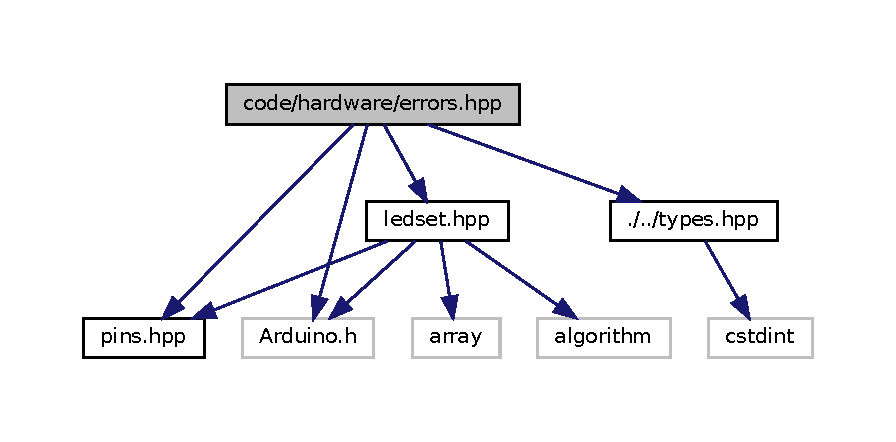
\includegraphics[width=350pt]{errors_8hpp__incl}
\end{center}
\end{figure}
This graph shows which files directly or indirectly include this file\+:\nopagebreak
\begin{figure}[H]
\begin{center}
\leavevmode
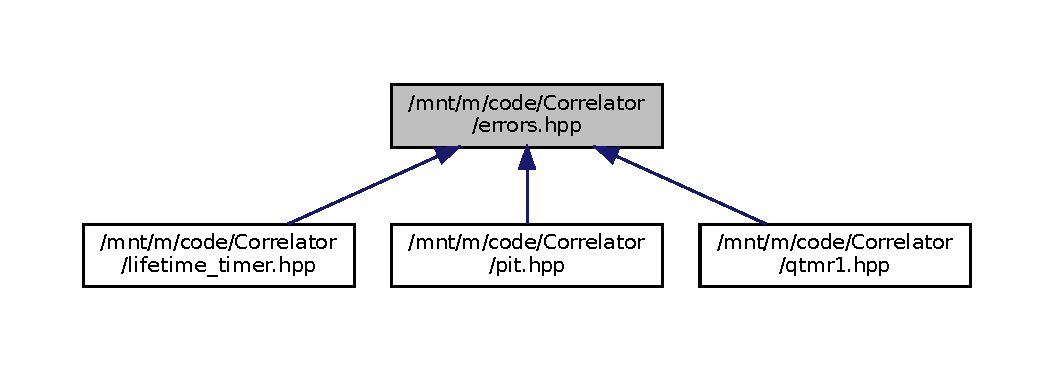
\includegraphics[width=350pt]{errors_8hpp__dep__incl}
\end{center}
\end{figure}
\subsection*{Classes}
\begin{DoxyCompactItemize}
\item 
class \hyperlink{classErrors}{Errors}
\end{DoxyCompactItemize}
\subsection*{Macros}
\begin{DoxyCompactItemize}
\item 
\#define \hyperlink{errors_8hpp_a0eb326048ed31037a6e5ec5634a6202e}{T\+E\+E\+N\+S\+Y\+\_\+\+M\+A\+X\+\_\+\+A\+L\+L\+O\+C\+A\+T\+I\+ON}~125000
\begin{DoxyCompactList}\small\item\em This file contain the Common Error Codes for Software-\/\+Hardware Interface. It defines the {\ttfamily Error\+\_\+t} and namespace {\ttfamily \hyperlink{classErrors}{Errors}} that are used to handle the errors and interact with the L\+ED dashboard. \end{DoxyCompactList}\end{DoxyCompactItemize}
\subsection*{Enumerations}
\begin{DoxyCompactItemize}
\item 
enum \hyperlink{errors_8hpp_a4e8c0d09726859e3d3369c0da5a1aa7f}{Error\+\_\+t} \{ \newline
\hyperlink{errors_8hpp_a4e8c0d09726859e3d3369c0da5a1aa7fa505a83f220c02df2f85c3810cd9ceb38}{Error\+\_\+t\+::\+Success} = 0, 
\hyperlink{errors_8hpp_a4e8c0d09726859e3d3369c0da5a1aa7fa8347bab2e74e4a640d76c916306a1a36}{Error\+\_\+t\+::\+Counter\+\_\+\+Overflow}, 
\hyperlink{errors_8hpp_a4e8c0d09726859e3d3369c0da5a1aa7fa02b02f5e5e61f24acdd91338b95997da}{Error\+\_\+t\+::\+Counter\+\_\+\+Underflow}, 
\hyperlink{errors_8hpp_a4e8c0d09726859e3d3369c0da5a1aa7fabe5edab59de4ea30531374e506b03822}{Error\+\_\+t\+::\+Precision}, 
\newline
\hyperlink{errors_8hpp_a4e8c0d09726859e3d3369c0da5a1aa7fa7e748bca7005cc737bad51b247997421}{Error\+\_\+t\+::\+Input\+\_\+\+Validation}, 
\hyperlink{errors_8hpp_a4e8c0d09726859e3d3369c0da5a1aa7fac7e40b9218d101cde2dc4c43b9fed0fe}{Error\+\_\+t\+::\+Generic\+\_\+\+Error}
 \}\begin{DoxyCompactList}\small\item\em Enumarates the error codes thrown by the different modules. \end{DoxyCompactList}
\end{DoxyCompactItemize}


\subsection{Macro Definition Documentation}
\mbox{\Hypertarget{errors_8hpp_a0eb326048ed31037a6e5ec5634a6202e}\label{errors_8hpp_a0eb326048ed31037a6e5ec5634a6202e}} 
\index{errors.\+hpp@{errors.\+hpp}!T\+E\+E\+N\+S\+Y\+\_\+\+M\+A\+X\+\_\+\+A\+L\+L\+O\+C\+A\+T\+I\+ON@{T\+E\+E\+N\+S\+Y\+\_\+\+M\+A\+X\+\_\+\+A\+L\+L\+O\+C\+A\+T\+I\+ON}}
\index{T\+E\+E\+N\+S\+Y\+\_\+\+M\+A\+X\+\_\+\+A\+L\+L\+O\+C\+A\+T\+I\+ON@{T\+E\+E\+N\+S\+Y\+\_\+\+M\+A\+X\+\_\+\+A\+L\+L\+O\+C\+A\+T\+I\+ON}!errors.\+hpp@{errors.\+hpp}}
\subsubsection{\texorpdfstring{T\+E\+E\+N\+S\+Y\+\_\+\+M\+A\+X\+\_\+\+A\+L\+L\+O\+C\+A\+T\+I\+ON}{TEENSY\_MAX\_ALLOCATION}}
{\footnotesize\ttfamily \#define T\+E\+E\+N\+S\+Y\+\_\+\+M\+A\+X\+\_\+\+A\+L\+L\+O\+C\+A\+T\+I\+ON~125000}



This file contain the Common Error Codes for Software-\/\+Hardware Interface. It defines the {\ttfamily Error\+\_\+t} and namespace {\ttfamily \hyperlink{classErrors}{Errors}} that are used to handle the errors and interact with the L\+ED dashboard. 

\begin{DoxyAuthor}{Author}
Yatharth Bhasin (github → yatharthb97) Maximum Allocations of 32-\/bit integers allowed on the microcontroller Teensy. 
\end{DoxyAuthor}


\subsection{Enumeration Type Documentation}
\mbox{\Hypertarget{errors_8hpp_a4e8c0d09726859e3d3369c0da5a1aa7f}\label{errors_8hpp_a4e8c0d09726859e3d3369c0da5a1aa7f}} 
\index{errors.\+hpp@{errors.\+hpp}!Error\+\_\+t@{Error\+\_\+t}}
\index{Error\+\_\+t@{Error\+\_\+t}!errors.\+hpp@{errors.\+hpp}}
\subsubsection{\texorpdfstring{Error\+\_\+t}{Error\_t}}
{\footnotesize\ttfamily enum \hyperlink{errors_8hpp_a4e8c0d09726859e3d3369c0da5a1aa7f}{Error\+\_\+t}\hspace{0.3cm}{\ttfamily [strong]}}



Enumarates the error codes thrown by the different modules. 

\begin{DoxyEnumFields}{Enumerator}
\raisebox{\heightof{T}}[0pt][0pt]{\index{Success@{Success}!errors.\+hpp@{errors.\+hpp}}\index{errors.\+hpp@{errors.\+hpp}!Success@{Success}}}\mbox{\Hypertarget{errors_8hpp_a4e8c0d09726859e3d3369c0da5a1aa7fa505a83f220c02df2f85c3810cd9ceb38}\label{errors_8hpp_a4e8c0d09726859e3d3369c0da5a1aa7fa505a83f220c02df2f85c3810cd9ceb38}} 
Success&No error. \\
\hline

\raisebox{\heightof{T}}[0pt][0pt]{\index{Counter\+\_\+\+Overflow@{Counter\+\_\+\+Overflow}!errors.\+hpp@{errors.\+hpp}}\index{errors.\+hpp@{errors.\+hpp}!Counter\+\_\+\+Overflow@{Counter\+\_\+\+Overflow}}}\mbox{\Hypertarget{errors_8hpp_a4e8c0d09726859e3d3369c0da5a1aa7fa8347bab2e74e4a640d76c916306a1a36}\label{errors_8hpp_a4e8c0d09726859e3d3369c0da5a1aa7fa8347bab2e74e4a640d76c916306a1a36}} 
Counter\+\_\+\+Overflow&Passed Value caused a counter overflow. \\
\hline

\raisebox{\heightof{T}}[0pt][0pt]{\index{Counter\+\_\+\+Underflow@{Counter\+\_\+\+Underflow}!errors.\+hpp@{errors.\+hpp}}\index{errors.\+hpp@{errors.\+hpp}!Counter\+\_\+\+Underflow@{Counter\+\_\+\+Underflow}}}\mbox{\Hypertarget{errors_8hpp_a4e8c0d09726859e3d3369c0da5a1aa7fa02b02f5e5e61f24acdd91338b95997da}\label{errors_8hpp_a4e8c0d09726859e3d3369c0da5a1aa7fa02b02f5e5e61f24acdd91338b95997da}} 
Counter\+\_\+\+Underflow&Passed Value caused a counter underflow. \\
\hline

\raisebox{\heightof{T}}[0pt][0pt]{\index{Precision@{Precision}!errors.\+hpp@{errors.\+hpp}}\index{errors.\+hpp@{errors.\+hpp}!Precision@{Precision}}}\mbox{\Hypertarget{errors_8hpp_a4e8c0d09726859e3d3369c0da5a1aa7fabe5edab59de4ea30531374e506b03822}\label{errors_8hpp_a4e8c0d09726859e3d3369c0da5a1aa7fabe5edab59de4ea30531374e506b03822}} 
Precision&Error generated when difference due to finite resolution is greater than acceptable. \\
\hline

\raisebox{\heightof{T}}[0pt][0pt]{\index{Input\+\_\+\+Validation@{Input\+\_\+\+Validation}!errors.\+hpp@{errors.\+hpp}}\index{errors.\+hpp@{errors.\+hpp}!Input\+\_\+\+Validation@{Input\+\_\+\+Validation}}}\mbox{\Hypertarget{errors_8hpp_a4e8c0d09726859e3d3369c0da5a1aa7fa7e748bca7005cc737bad51b247997421}\label{errors_8hpp_a4e8c0d09726859e3d3369c0da5a1aa7fa7e748bca7005cc737bad51b247997421}} 
Input\+\_\+\+Validation&Input validation failed. \\
\hline

\raisebox{\heightof{T}}[0pt][0pt]{\index{Generic\+\_\+\+Error@{Generic\+\_\+\+Error}!errors.\+hpp@{errors.\+hpp}}\index{errors.\+hpp@{errors.\+hpp}!Generic\+\_\+\+Error@{Generic\+\_\+\+Error}}}\mbox{\Hypertarget{errors_8hpp_a4e8c0d09726859e3d3369c0da5a1aa7fac7e40b9218d101cde2dc4c43b9fed0fe}\label{errors_8hpp_a4e8c0d09726859e3d3369c0da5a1aa7fac7e40b9218d101cde2dc4c43b9fed0fe}} 
Generic\+\_\+\+Error&Only here for development and debugging. \\
\hline

\end{DoxyEnumFields}

\hypertarget{interarrival_8hpp}{}\section{code/hardware/interarrival.hpp File Reference}
\label{interarrival_8hpp}\index{code/hardware/interarrival.\+hpp@{code/hardware/interarrival.\+hpp}}
{\ttfamily \#include $<$type\+\_\+traits$>$}\newline
{\ttfamily \#include \char`\"{}./../software/monitor\+\_\+channel.\+hpp\char`\"{}}\newline
Include dependency graph for interarrival.\+hpp\+:
\nopagebreak
\begin{figure}[H]
\begin{center}
\leavevmode
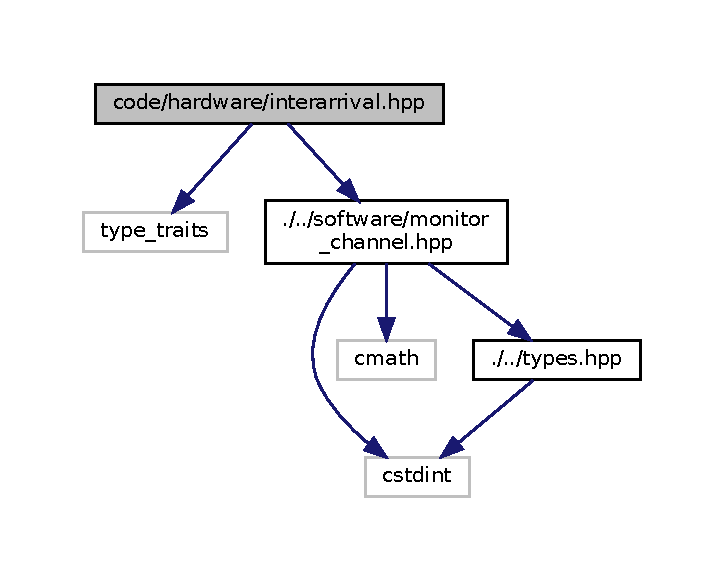
\includegraphics[width=348pt]{d0/d6d/interarrival_8hpp__incl}
\end{center}
\end{figure}
This graph shows which files directly or indirectly include this file\+:
\nopagebreak
\begin{figure}[H]
\begin{center}
\leavevmode
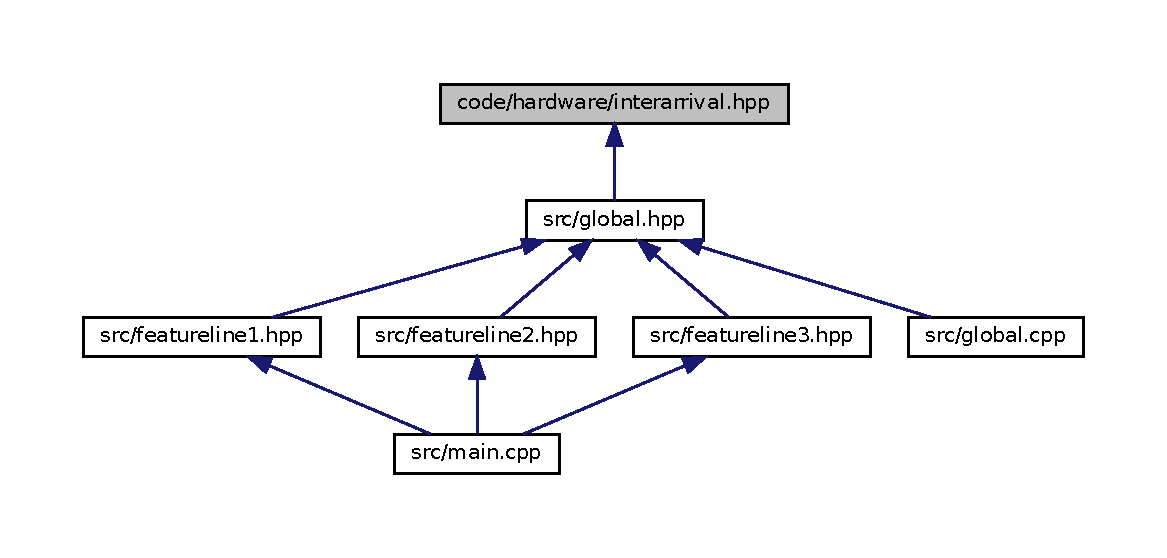
\includegraphics[width=350pt]{df/df8/interarrival_8hpp__dep__incl}
\end{center}
\end{figure}
\subsection*{Classes}
\begin{DoxyCompactItemize}
\item 
class \hyperlink{classInterArrivalTime}{Inter\+Arrival\+Time$<$ Counter\+Type, C\+P\+U\+Tick\+Type $>$}
\end{DoxyCompactItemize}
\subsection*{Macros}
\begin{DoxyCompactItemize}
\item 
\#define \hyperlink{interarrival_8hpp_a10bd13bb1bfb1df851899b75e175035b}{I\+N\+T\+E\+R\+A\+R\+R\+I\+V\+A\+L\+T\+I\+M\+E\+\_\+\+M\+I\+N\+M\+A\+X\+\_\+\+S\+T\+A\+T\+I\+S\+T\+I\+CS}~0
\end{DoxyCompactItemize}


\subsection{Macro Definition Documentation}
\mbox{\Hypertarget{interarrival_8hpp_a10bd13bb1bfb1df851899b75e175035b}\label{interarrival_8hpp_a10bd13bb1bfb1df851899b75e175035b}} 
\index{interarrival.\+hpp@{interarrival.\+hpp}!I\+N\+T\+E\+R\+A\+R\+R\+I\+V\+A\+L\+T\+I\+M\+E\+\_\+\+M\+I\+N\+M\+A\+X\+\_\+\+S\+T\+A\+T\+I\+S\+T\+I\+CS@{I\+N\+T\+E\+R\+A\+R\+R\+I\+V\+A\+L\+T\+I\+M\+E\+\_\+\+M\+I\+N\+M\+A\+X\+\_\+\+S\+T\+A\+T\+I\+S\+T\+I\+CS}}
\index{I\+N\+T\+E\+R\+A\+R\+R\+I\+V\+A\+L\+T\+I\+M\+E\+\_\+\+M\+I\+N\+M\+A\+X\+\_\+\+S\+T\+A\+T\+I\+S\+T\+I\+CS@{I\+N\+T\+E\+R\+A\+R\+R\+I\+V\+A\+L\+T\+I\+M\+E\+\_\+\+M\+I\+N\+M\+A\+X\+\_\+\+S\+T\+A\+T\+I\+S\+T\+I\+CS}!interarrival.\+hpp@{interarrival.\+hpp}}
\subsubsection{\texorpdfstring{I\+N\+T\+E\+R\+A\+R\+R\+I\+V\+A\+L\+T\+I\+M\+E\+\_\+\+M\+I\+N\+M\+A\+X\+\_\+\+S\+T\+A\+T\+I\+S\+T\+I\+CS}{INTERARRIVALTIME\_MINMAX\_STATISTICS}}
{\footnotesize\ttfamily \#define I\+N\+T\+E\+R\+A\+R\+R\+I\+V\+A\+L\+T\+I\+M\+E\+\_\+\+M\+I\+N\+M\+A\+X\+\_\+\+S\+T\+A\+T\+I\+S\+T\+I\+CS~0}


\hypertarget{ledpanel_8hpp}{}\section{code/hardware/ledpanel.hpp File Reference}
\label{ledpanel_8hpp}\index{code/hardware/ledpanel.\+hpp@{code/hardware/ledpanel.\+hpp}}
{\ttfamily \#include \char`\"{}ledset.\+hpp\char`\"{}}\newline
Include dependency graph for ledpanel.\+hpp\+:\nopagebreak
\begin{figure}[H]
\begin{center}
\leavevmode
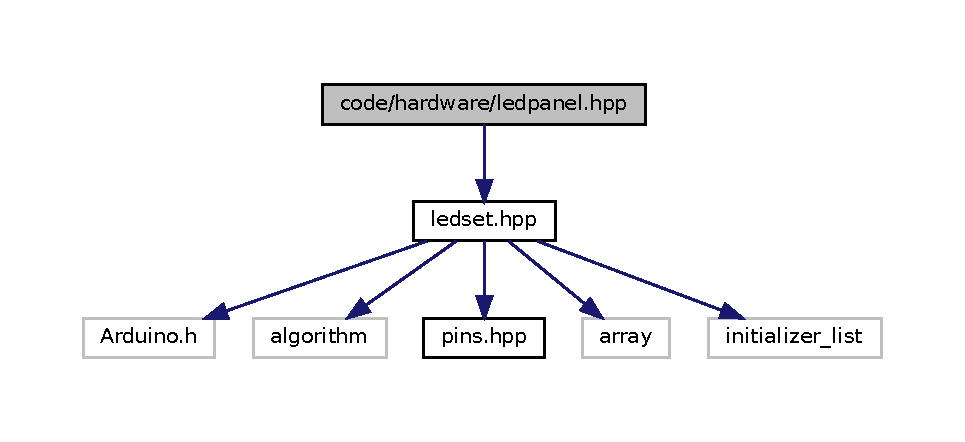
\includegraphics[width=350pt]{da/dde/ledpanel_8hpp__incl}
\end{center}
\end{figure}
This graph shows which files directly or indirectly include this file\+:
\nopagebreak
\begin{figure}[H]
\begin{center}
\leavevmode
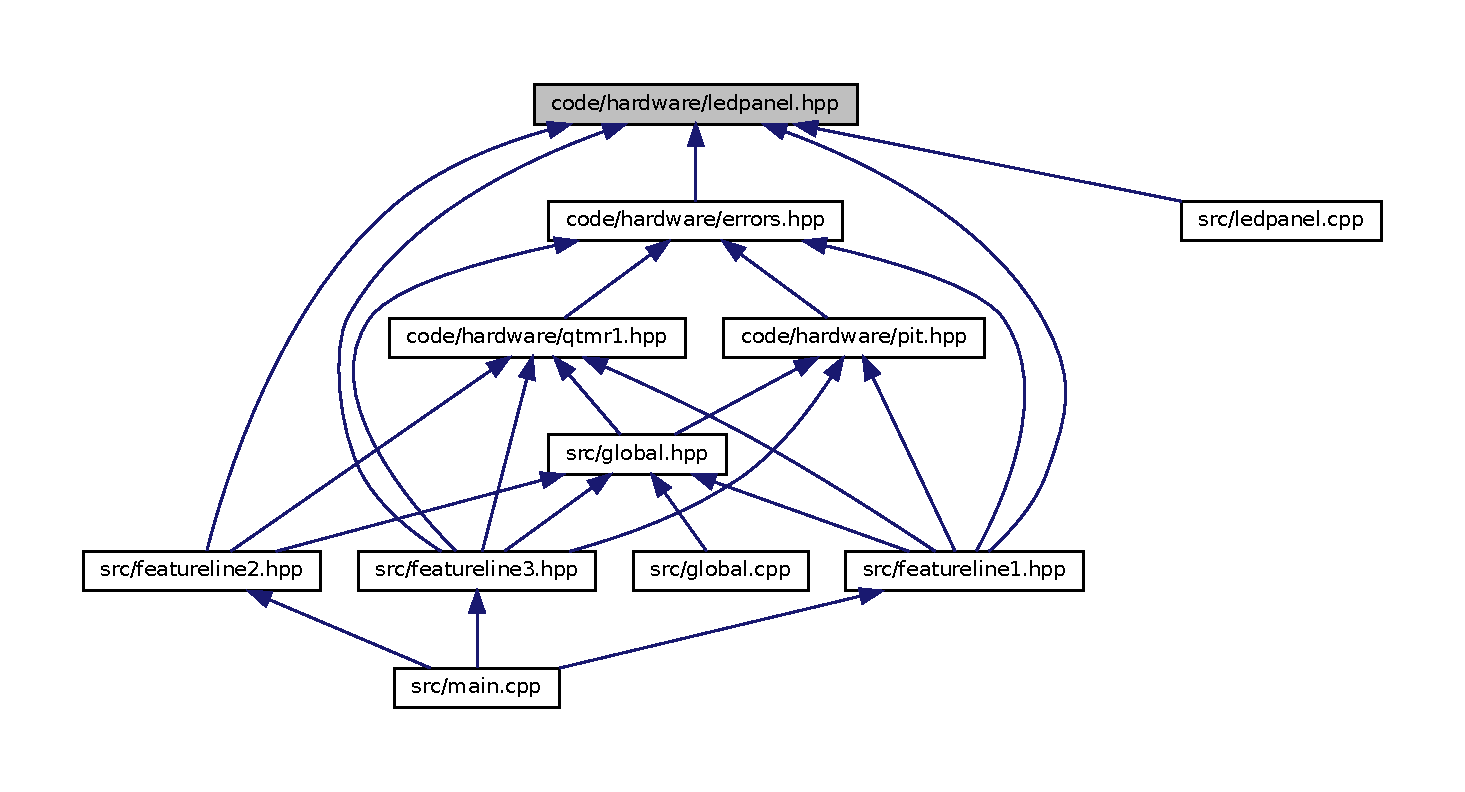
\includegraphics[width=350pt]{d4/d87/ledpanel_8hpp__dep__incl}
\end{center}
\end{figure}

\hypertarget{ledset_8hpp}{}\section{code/hardware/ledset.hpp File Reference}
\label{ledset_8hpp}\index{code/hardware/ledset.\+hpp@{code/hardware/ledset.\+hpp}}
{\ttfamily \#include $<$Arduino.\+h$>$}\newline
{\ttfamily \#include $<$algorithm$>$}\newline
{\ttfamily \#include \char`\"{}pins.\+hpp\char`\"{}}\newline
{\ttfamily \#include $<$array$>$}\newline
{\ttfamily \#include $<$initializer\+\_\+list$>$}\newline
Include dependency graph for ledset.\+hpp\+:\nopagebreak
\begin{figure}[H]
\begin{center}
\leavevmode
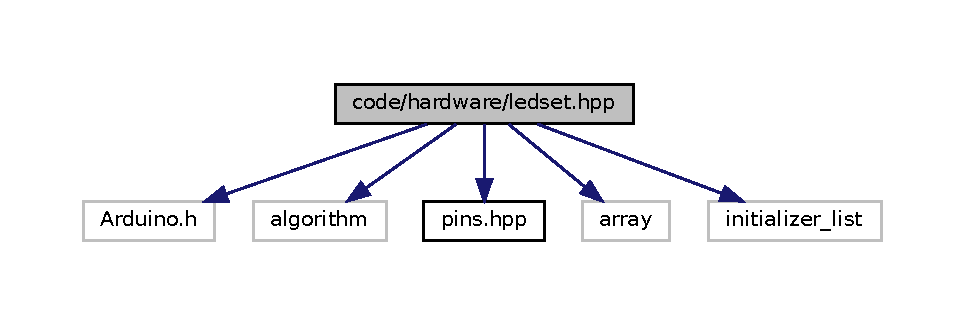
\includegraphics[width=350pt]{ledset_8hpp__incl}
\end{center}
\end{figure}
This graph shows which files directly or indirectly include this file\+:\nopagebreak
\begin{figure}[H]
\begin{center}
\leavevmode
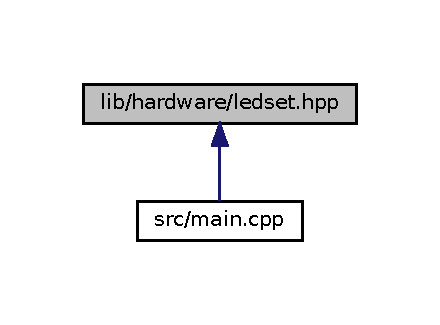
\includegraphics[width=350pt]{ledset_8hpp__dep__incl}
\end{center}
\end{figure}
\subsection*{Classes}
\begin{DoxyCompactItemize}
\item 
class \hyperlink{classLEDSet}{L\+E\+D\+Set$<$ S\+E\+T\+\_\+\+S\+I\+Z\+E $>$}
\end{DoxyCompactItemize}

\hypertarget{lifetime__timer_8hpp}{}\section{/mnt/m/code/\+Correlator/lifetime\+\_\+timer.hpp File Reference}
\label{lifetime__timer_8hpp}\index{/mnt/m/code/\+Correlator/lifetime\+\_\+timer.\+hpp@{/mnt/m/code/\+Correlator/lifetime\+\_\+timer.\+hpp}}
{\ttfamily \#include \char`\"{}errors.\+hpp\char`\"{}}\newline
Include dependency graph for lifetime\+\_\+timer.\+hpp\+:
\nopagebreak
\begin{figure}[H]
\begin{center}
\leavevmode
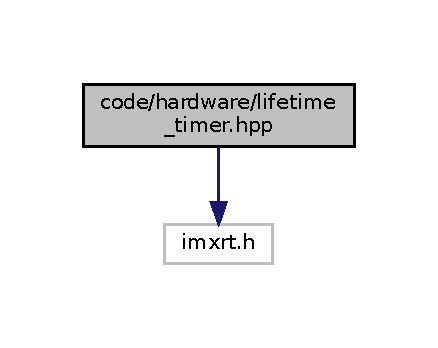
\includegraphics[width=210pt]{lifetime__timer_8hpp__incl}
\end{center}
\end{figure}
\subsection*{Classes}
\begin{DoxyCompactItemize}
\item 
class \hyperlink{classPIT__LifetimeTimer}{P\+I\+T\+\_\+\+Lifetime\+Timer}
\begin{DoxyCompactList}\small\item\em Interface for using the \char`\"{}\+Life Time T\+Imer\char`\"{} functionality of the Periodic Interrut Timer on Teensy 4.\+x microcontrollers. The module uses Channel 0 and 1 of the 4 P\+IT channels. \end{DoxyCompactList}\end{DoxyCompactItemize}

\hypertarget{perf__counter_8hpp}{}\section{code/hardware/perf\+\_\+counter.hpp File Reference}
\label{perf__counter_8hpp}\index{code/hardware/perf\+\_\+counter.\+hpp@{code/hardware/perf\+\_\+counter.\+hpp}}
{\ttfamily \#include $<$imxrt.\+h$>$}\newline
{\ttfamily \#include $<$Arduino.\+h$>$}\newline
Include dependency graph for perf\+\_\+counter.\+hpp\+:\nopagebreak
\begin{figure}[H]
\begin{center}
\leavevmode
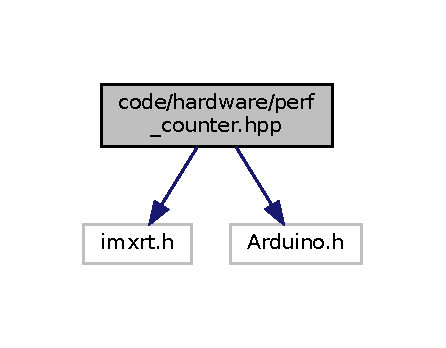
\includegraphics[width=214pt]{perf__counter_8hpp__incl}
\end{center}
\end{figure}
This graph shows which files directly or indirectly include this file\+:\nopagebreak
\begin{figure}[H]
\begin{center}
\leavevmode
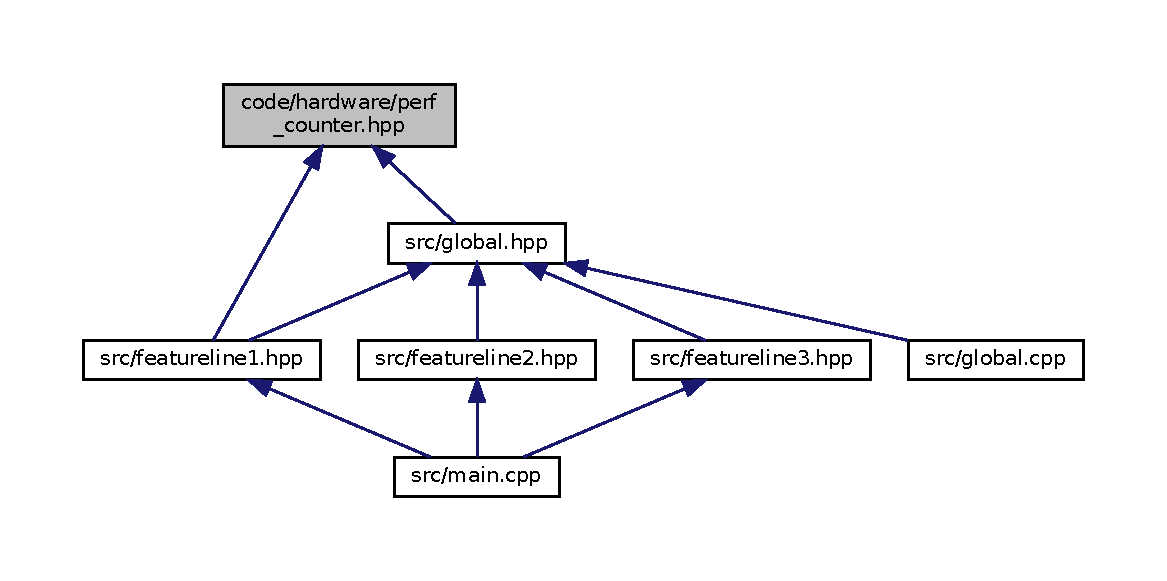
\includegraphics[width=350pt]{perf__counter_8hpp__dep__incl}
\end{center}
\end{figure}
\subsection*{Classes}
\begin{DoxyCompactItemize}
\item 
class \hyperlink{classPerfCounter}{Perf\+Counter}
\begin{DoxyCompactList}\small\item\em Performance Counter class for teensy 4.\+1 microcontrollers. \end{DoxyCompactList}\end{DoxyCompactItemize}

\hypertarget{pins_8hpp}{}\section{code/hardware/pins.hpp File Reference}
\label{pins_8hpp}\index{code/hardware/pins.\+hpp@{code/hardware/pins.\+hpp}}
This graph shows which files directly or indirectly include this file\+:\nopagebreak
\begin{figure}[H]
\begin{center}
\leavevmode
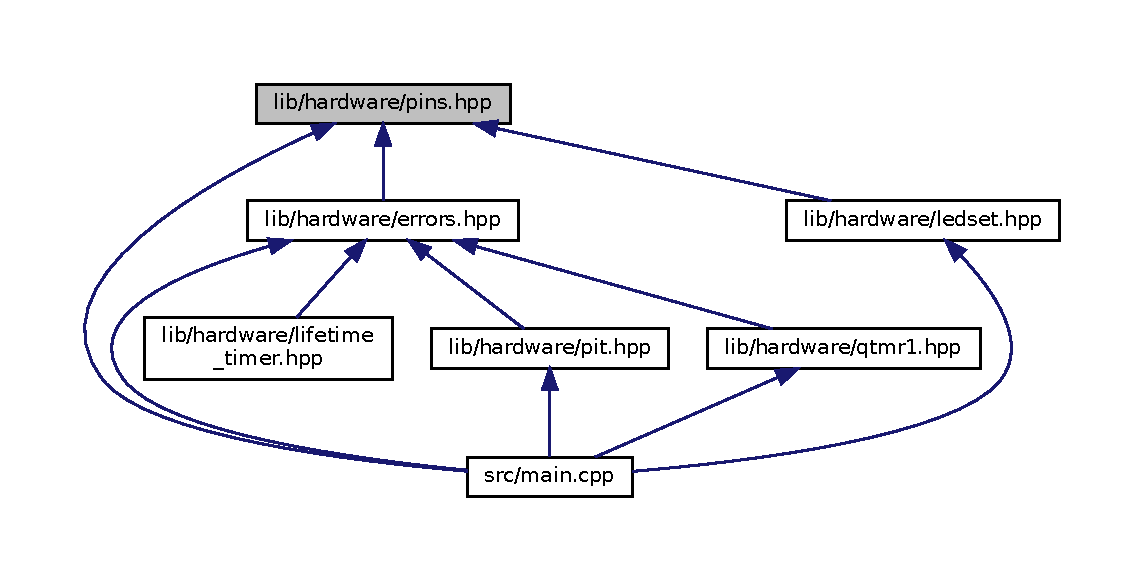
\includegraphics[width=350pt]{pins_8hpp__dep__incl}
\end{center}
\end{figure}
\subsection*{Variables}
\begin{DoxyCompactItemize}
\item 
const int \hyperlink{pins_8hpp_a735f426a390e22c0050b964328c5e06f}{L\+E\+D\+\_\+\+R\+ED} = 41
\item 
const int \hyperlink{pins_8hpp_a8046eca6ddcbe578777cfde489622a13}{L\+E\+D\+\_\+\+B\+L\+UE} = 40
\item 
const int \hyperlink{pins_8hpp_af338796c804fbfe2e9fd4d249e3c5004}{L\+E\+D\+\_\+\+Y\+E\+L\+L\+OW} = 22
\item 
const int \hyperlink{pins_8hpp_a1be903f86639d50fb6ed02a0dbbe0e2c}{L\+E\+D\+\_\+\+W\+H\+I\+TE} = 23
\item 
const int \hyperlink{pins_8hpp_a8d7df4222b2fde6205bebffc5a0ae070}{L\+E\+D\+\_\+\+G\+R\+E\+EN} = 24
\item 
const int \hyperlink{pins_8hpp_a6a5a6d5ec94efcbf2c8bffa0b660f013}{S\+A\+F\+E\+\_\+\+I\+N\+P\+U\+T\+\_\+\+D\+U\+M\+P\+\_\+\+P\+IN} = 0
\item 
const int \hyperlink{pins_8hpp_a2b2fb4f846b45d396215a25f949a1bc7}{S\+A\+F\+E\+\_\+\+O\+U\+T\+P\+U\+T\+\_\+\+D\+U\+M\+P\+\_\+\+P\+IN} = 0
\item 
const int \hyperlink{pins_8hpp_a5017daf6b9fb9330e86878ec983ed163}{T\+T\+L\+\_\+\+C\+\_\+\+P\+U\+L\+S\+E\+\_\+\+I\+N\+P\+U\+T\+\_\+\+P\+IN} = 10
\item 
const int \hyperlink{pins_8hpp_a01ff5c1b8f46ca9504e840c5aaf9fd64}{E\+R\+\_\+\+P\+R\+E\+C\+I\+S\+I\+O\+N\+\_\+\+P\+IN} = \hyperlink{pins_8hpp_a8046eca6ddcbe578777cfde489622a13}{L\+E\+D\+\_\+\+B\+L\+UE}
\item 
const int \hyperlink{pins_8hpp_ae73bc7e4372631b754daf933169b2a16}{E\+R\+\_\+\+O\+V\+E\+R\+F\+L\+O\+W\+\_\+\+P\+IN} = \hyperlink{pins_8hpp_a1be903f86639d50fb6ed02a0dbbe0e2c}{L\+E\+D\+\_\+\+W\+H\+I\+TE}
\item 
const int \hyperlink{pins_8hpp_a3bf66a7f687091434a704c61863c3141}{E\+R\+\_\+\+I\+N\+P\+U\+T\+\_\+\+V\+A\+L\+I\+D\+A\+T\+I\+ON} = \hyperlink{pins_8hpp_a735f426a390e22c0050b964328c5e06f}{L\+E\+D\+\_\+\+R\+ED}
\item 
const int \hyperlink{pins_8hpp_a3bceb7a516452849c8b6292b69e4fb71}{S\+E\+T\+U\+P\+\_\+\+L\+ED} = \hyperlink{pins_8hpp_a735f426a390e22c0050b964328c5e06f}{L\+E\+D\+\_\+\+R\+ED}
\item 
const int \hyperlink{pins_8hpp_a1c1c13275493f645825a60c5710264e5}{L\+O\+O\+P\+\_\+\+L\+ED} = \hyperlink{pins_8hpp_a8d7df4222b2fde6205bebffc5a0ae070}{L\+E\+D\+\_\+\+G\+R\+E\+EN}
\end{DoxyCompactItemize}


\subsection{Variable Documentation}
\mbox{\Hypertarget{pins_8hpp_a3bf66a7f687091434a704c61863c3141}\label{pins_8hpp_a3bf66a7f687091434a704c61863c3141}} 
\index{pins.\+hpp@{pins.\+hpp}!E\+R\+\_\+\+I\+N\+P\+U\+T\+\_\+\+V\+A\+L\+I\+D\+A\+T\+I\+ON@{E\+R\+\_\+\+I\+N\+P\+U\+T\+\_\+\+V\+A\+L\+I\+D\+A\+T\+I\+ON}}
\index{E\+R\+\_\+\+I\+N\+P\+U\+T\+\_\+\+V\+A\+L\+I\+D\+A\+T\+I\+ON@{E\+R\+\_\+\+I\+N\+P\+U\+T\+\_\+\+V\+A\+L\+I\+D\+A\+T\+I\+ON}!pins.\+hpp@{pins.\+hpp}}
\subsubsection{\texorpdfstring{E\+R\+\_\+\+I\+N\+P\+U\+T\+\_\+\+V\+A\+L\+I\+D\+A\+T\+I\+ON}{ER\_INPUT\_VALIDATION}}
{\footnotesize\ttfamily const int E\+R\+\_\+\+I\+N\+P\+U\+T\+\_\+\+V\+A\+L\+I\+D\+A\+T\+I\+ON = \hyperlink{pins_8hpp_a735f426a390e22c0050b964328c5e06f}{L\+E\+D\+\_\+\+R\+ED}}

\mbox{\Hypertarget{pins_8hpp_ae73bc7e4372631b754daf933169b2a16}\label{pins_8hpp_ae73bc7e4372631b754daf933169b2a16}} 
\index{pins.\+hpp@{pins.\+hpp}!E\+R\+\_\+\+O\+V\+E\+R\+F\+L\+O\+W\+\_\+\+P\+IN@{E\+R\+\_\+\+O\+V\+E\+R\+F\+L\+O\+W\+\_\+\+P\+IN}}
\index{E\+R\+\_\+\+O\+V\+E\+R\+F\+L\+O\+W\+\_\+\+P\+IN@{E\+R\+\_\+\+O\+V\+E\+R\+F\+L\+O\+W\+\_\+\+P\+IN}!pins.\+hpp@{pins.\+hpp}}
\subsubsection{\texorpdfstring{E\+R\+\_\+\+O\+V\+E\+R\+F\+L\+O\+W\+\_\+\+P\+IN}{ER\_OVERFLOW\_PIN}}
{\footnotesize\ttfamily const int E\+R\+\_\+\+O\+V\+E\+R\+F\+L\+O\+W\+\_\+\+P\+IN = \hyperlink{pins_8hpp_a1be903f86639d50fb6ed02a0dbbe0e2c}{L\+E\+D\+\_\+\+W\+H\+I\+TE}}

\mbox{\Hypertarget{pins_8hpp_a01ff5c1b8f46ca9504e840c5aaf9fd64}\label{pins_8hpp_a01ff5c1b8f46ca9504e840c5aaf9fd64}} 
\index{pins.\+hpp@{pins.\+hpp}!E\+R\+\_\+\+P\+R\+E\+C\+I\+S\+I\+O\+N\+\_\+\+P\+IN@{E\+R\+\_\+\+P\+R\+E\+C\+I\+S\+I\+O\+N\+\_\+\+P\+IN}}
\index{E\+R\+\_\+\+P\+R\+E\+C\+I\+S\+I\+O\+N\+\_\+\+P\+IN@{E\+R\+\_\+\+P\+R\+E\+C\+I\+S\+I\+O\+N\+\_\+\+P\+IN}!pins.\+hpp@{pins.\+hpp}}
\subsubsection{\texorpdfstring{E\+R\+\_\+\+P\+R\+E\+C\+I\+S\+I\+O\+N\+\_\+\+P\+IN}{ER\_PRECISION\_PIN}}
{\footnotesize\ttfamily const int E\+R\+\_\+\+P\+R\+E\+C\+I\+S\+I\+O\+N\+\_\+\+P\+IN = \hyperlink{pins_8hpp_a8046eca6ddcbe578777cfde489622a13}{L\+E\+D\+\_\+\+B\+L\+UE}}

\mbox{\Hypertarget{pins_8hpp_a8046eca6ddcbe578777cfde489622a13}\label{pins_8hpp_a8046eca6ddcbe578777cfde489622a13}} 
\index{pins.\+hpp@{pins.\+hpp}!L\+E\+D\+\_\+\+B\+L\+UE@{L\+E\+D\+\_\+\+B\+L\+UE}}
\index{L\+E\+D\+\_\+\+B\+L\+UE@{L\+E\+D\+\_\+\+B\+L\+UE}!pins.\+hpp@{pins.\+hpp}}
\subsubsection{\texorpdfstring{L\+E\+D\+\_\+\+B\+L\+UE}{LED\_BLUE}}
{\footnotesize\ttfamily const int L\+E\+D\+\_\+\+B\+L\+UE = 40}

\mbox{\Hypertarget{pins_8hpp_a8d7df4222b2fde6205bebffc5a0ae070}\label{pins_8hpp_a8d7df4222b2fde6205bebffc5a0ae070}} 
\index{pins.\+hpp@{pins.\+hpp}!L\+E\+D\+\_\+\+G\+R\+E\+EN@{L\+E\+D\+\_\+\+G\+R\+E\+EN}}
\index{L\+E\+D\+\_\+\+G\+R\+E\+EN@{L\+E\+D\+\_\+\+G\+R\+E\+EN}!pins.\+hpp@{pins.\+hpp}}
\subsubsection{\texorpdfstring{L\+E\+D\+\_\+\+G\+R\+E\+EN}{LED\_GREEN}}
{\footnotesize\ttfamily const int L\+E\+D\+\_\+\+G\+R\+E\+EN = 24}

\mbox{\Hypertarget{pins_8hpp_a735f426a390e22c0050b964328c5e06f}\label{pins_8hpp_a735f426a390e22c0050b964328c5e06f}} 
\index{pins.\+hpp@{pins.\+hpp}!L\+E\+D\+\_\+\+R\+ED@{L\+E\+D\+\_\+\+R\+ED}}
\index{L\+E\+D\+\_\+\+R\+ED@{L\+E\+D\+\_\+\+R\+ED}!pins.\+hpp@{pins.\+hpp}}
\subsubsection{\texorpdfstring{L\+E\+D\+\_\+\+R\+ED}{LED\_RED}}
{\footnotesize\ttfamily const int L\+E\+D\+\_\+\+R\+ED = 41}

\mbox{\Hypertarget{pins_8hpp_a1be903f86639d50fb6ed02a0dbbe0e2c}\label{pins_8hpp_a1be903f86639d50fb6ed02a0dbbe0e2c}} 
\index{pins.\+hpp@{pins.\+hpp}!L\+E\+D\+\_\+\+W\+H\+I\+TE@{L\+E\+D\+\_\+\+W\+H\+I\+TE}}
\index{L\+E\+D\+\_\+\+W\+H\+I\+TE@{L\+E\+D\+\_\+\+W\+H\+I\+TE}!pins.\+hpp@{pins.\+hpp}}
\subsubsection{\texorpdfstring{L\+E\+D\+\_\+\+W\+H\+I\+TE}{LED\_WHITE}}
{\footnotesize\ttfamily const int L\+E\+D\+\_\+\+W\+H\+I\+TE = 23}

\mbox{\Hypertarget{pins_8hpp_af338796c804fbfe2e9fd4d249e3c5004}\label{pins_8hpp_af338796c804fbfe2e9fd4d249e3c5004}} 
\index{pins.\+hpp@{pins.\+hpp}!L\+E\+D\+\_\+\+Y\+E\+L\+L\+OW@{L\+E\+D\+\_\+\+Y\+E\+L\+L\+OW}}
\index{L\+E\+D\+\_\+\+Y\+E\+L\+L\+OW@{L\+E\+D\+\_\+\+Y\+E\+L\+L\+OW}!pins.\+hpp@{pins.\+hpp}}
\subsubsection{\texorpdfstring{L\+E\+D\+\_\+\+Y\+E\+L\+L\+OW}{LED\_YELLOW}}
{\footnotesize\ttfamily const int L\+E\+D\+\_\+\+Y\+E\+L\+L\+OW = 22}

\mbox{\Hypertarget{pins_8hpp_a1c1c13275493f645825a60c5710264e5}\label{pins_8hpp_a1c1c13275493f645825a60c5710264e5}} 
\index{pins.\+hpp@{pins.\+hpp}!L\+O\+O\+P\+\_\+\+L\+ED@{L\+O\+O\+P\+\_\+\+L\+ED}}
\index{L\+O\+O\+P\+\_\+\+L\+ED@{L\+O\+O\+P\+\_\+\+L\+ED}!pins.\+hpp@{pins.\+hpp}}
\subsubsection{\texorpdfstring{L\+O\+O\+P\+\_\+\+L\+ED}{LOOP\_LED}}
{\footnotesize\ttfamily const int L\+O\+O\+P\+\_\+\+L\+ED = \hyperlink{pins_8hpp_a8d7df4222b2fde6205bebffc5a0ae070}{L\+E\+D\+\_\+\+G\+R\+E\+EN}}

\mbox{\Hypertarget{pins_8hpp_a6a5a6d5ec94efcbf2c8bffa0b660f013}\label{pins_8hpp_a6a5a6d5ec94efcbf2c8bffa0b660f013}} 
\index{pins.\+hpp@{pins.\+hpp}!S\+A\+F\+E\+\_\+\+I\+N\+P\+U\+T\+\_\+\+D\+U\+M\+P\+\_\+\+P\+IN@{S\+A\+F\+E\+\_\+\+I\+N\+P\+U\+T\+\_\+\+D\+U\+M\+P\+\_\+\+P\+IN}}
\index{S\+A\+F\+E\+\_\+\+I\+N\+P\+U\+T\+\_\+\+D\+U\+M\+P\+\_\+\+P\+IN@{S\+A\+F\+E\+\_\+\+I\+N\+P\+U\+T\+\_\+\+D\+U\+M\+P\+\_\+\+P\+IN}!pins.\+hpp@{pins.\+hpp}}
\subsubsection{\texorpdfstring{S\+A\+F\+E\+\_\+\+I\+N\+P\+U\+T\+\_\+\+D\+U\+M\+P\+\_\+\+P\+IN}{SAFE\_INPUT\_DUMP\_PIN}}
{\footnotesize\ttfamily const int S\+A\+F\+E\+\_\+\+I\+N\+P\+U\+T\+\_\+\+D\+U\+M\+P\+\_\+\+P\+IN = 0}

\mbox{\Hypertarget{pins_8hpp_a2b2fb4f846b45d396215a25f949a1bc7}\label{pins_8hpp_a2b2fb4f846b45d396215a25f949a1bc7}} 
\index{pins.\+hpp@{pins.\+hpp}!S\+A\+F\+E\+\_\+\+O\+U\+T\+P\+U\+T\+\_\+\+D\+U\+M\+P\+\_\+\+P\+IN@{S\+A\+F\+E\+\_\+\+O\+U\+T\+P\+U\+T\+\_\+\+D\+U\+M\+P\+\_\+\+P\+IN}}
\index{S\+A\+F\+E\+\_\+\+O\+U\+T\+P\+U\+T\+\_\+\+D\+U\+M\+P\+\_\+\+P\+IN@{S\+A\+F\+E\+\_\+\+O\+U\+T\+P\+U\+T\+\_\+\+D\+U\+M\+P\+\_\+\+P\+IN}!pins.\+hpp@{pins.\+hpp}}
\subsubsection{\texorpdfstring{S\+A\+F\+E\+\_\+\+O\+U\+T\+P\+U\+T\+\_\+\+D\+U\+M\+P\+\_\+\+P\+IN}{SAFE\_OUTPUT\_DUMP\_PIN}}
{\footnotesize\ttfamily const int S\+A\+F\+E\+\_\+\+O\+U\+T\+P\+U\+T\+\_\+\+D\+U\+M\+P\+\_\+\+P\+IN = 0}

\mbox{\Hypertarget{pins_8hpp_a3bceb7a516452849c8b6292b69e4fb71}\label{pins_8hpp_a3bceb7a516452849c8b6292b69e4fb71}} 
\index{pins.\+hpp@{pins.\+hpp}!S\+E\+T\+U\+P\+\_\+\+L\+ED@{S\+E\+T\+U\+P\+\_\+\+L\+ED}}
\index{S\+E\+T\+U\+P\+\_\+\+L\+ED@{S\+E\+T\+U\+P\+\_\+\+L\+ED}!pins.\+hpp@{pins.\+hpp}}
\subsubsection{\texorpdfstring{S\+E\+T\+U\+P\+\_\+\+L\+ED}{SETUP\_LED}}
{\footnotesize\ttfamily const int S\+E\+T\+U\+P\+\_\+\+L\+ED = \hyperlink{pins_8hpp_a735f426a390e22c0050b964328c5e06f}{L\+E\+D\+\_\+\+R\+ED}}

\mbox{\Hypertarget{pins_8hpp_a5017daf6b9fb9330e86878ec983ed163}\label{pins_8hpp_a5017daf6b9fb9330e86878ec983ed163}} 
\index{pins.\+hpp@{pins.\+hpp}!T\+T\+L\+\_\+\+C\+\_\+\+P\+U\+L\+S\+E\+\_\+\+I\+N\+P\+U\+T\+\_\+\+P\+IN@{T\+T\+L\+\_\+\+C\+\_\+\+P\+U\+L\+S\+E\+\_\+\+I\+N\+P\+U\+T\+\_\+\+P\+IN}}
\index{T\+T\+L\+\_\+\+C\+\_\+\+P\+U\+L\+S\+E\+\_\+\+I\+N\+P\+U\+T\+\_\+\+P\+IN@{T\+T\+L\+\_\+\+C\+\_\+\+P\+U\+L\+S\+E\+\_\+\+I\+N\+P\+U\+T\+\_\+\+P\+IN}!pins.\+hpp@{pins.\+hpp}}
\subsubsection{\texorpdfstring{T\+T\+L\+\_\+\+C\+\_\+\+P\+U\+L\+S\+E\+\_\+\+I\+N\+P\+U\+T\+\_\+\+P\+IN}{TTL\_C\_PULSE\_INPUT\_PIN}}
{\footnotesize\ttfamily const int T\+T\+L\+\_\+\+C\+\_\+\+P\+U\+L\+S\+E\+\_\+\+I\+N\+P\+U\+T\+\_\+\+P\+IN = 10}


\hypertarget{pit_8hpp}{}\section{/mnt/m/code/\+Correlator/pit.hpp File Reference}
\label{pit_8hpp}\index{/mnt/m/code/\+Correlator/pit.\+hpp@{/mnt/m/code/\+Correlator/pit.\+hpp}}
{\ttfamily \#include \char`\"{}errors.\+hpp\char`\"{}}\newline
Include dependency graph for pit.\+hpp\+:\nopagebreak
\begin{figure}[H]
\begin{center}
\leavevmode
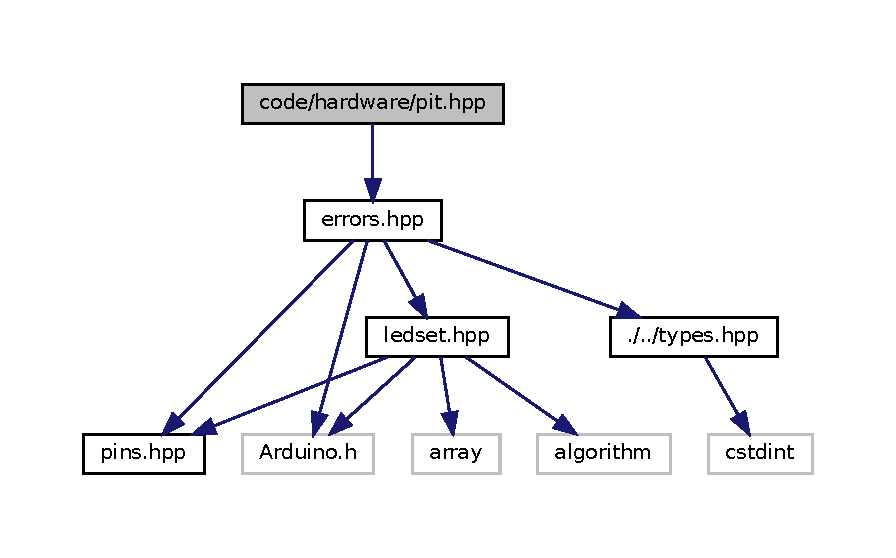
\includegraphics[width=210pt]{pit_8hpp__incl}
\end{center}
\end{figure}
\subsection*{Classes}
\begin{DoxyCompactItemize}
\item 
class \hyperlink{classPITController}{P\+I\+T\+Controller$<$ Ch\+I\+D $>$}
\begin{DoxyCompactList}\small\item\em Interface for P\+IT timers on Teensy 4.\+x microcontrollers. \end{DoxyCompactList}\end{DoxyCompactItemize}

\hypertarget{qtmr1_8hpp}{}\section{code/hardware/qtmr1.hpp File Reference}
\label{qtmr1_8hpp}\index{code/hardware/qtmr1.\+hpp@{code/hardware/qtmr1.\+hpp}}
{\ttfamily \#include \char`\"{}errors.\+hpp\char`\"{}}\newline
Include dependency graph for qtmr1.\+hpp\+:\nopagebreak
\begin{figure}[H]
\begin{center}
\leavevmode
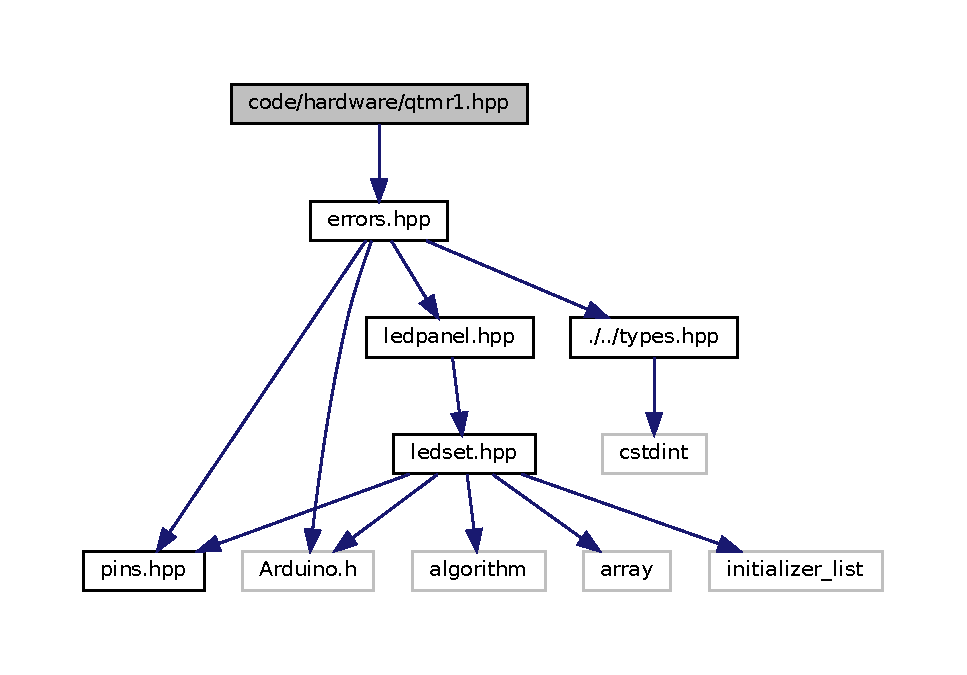
\includegraphics[width=350pt]{d5/d22/qtmr1_8hpp__incl}
\end{center}
\end{figure}
This graph shows which files directly or indirectly include this file\+:
\nopagebreak
\begin{figure}[H]
\begin{center}
\leavevmode
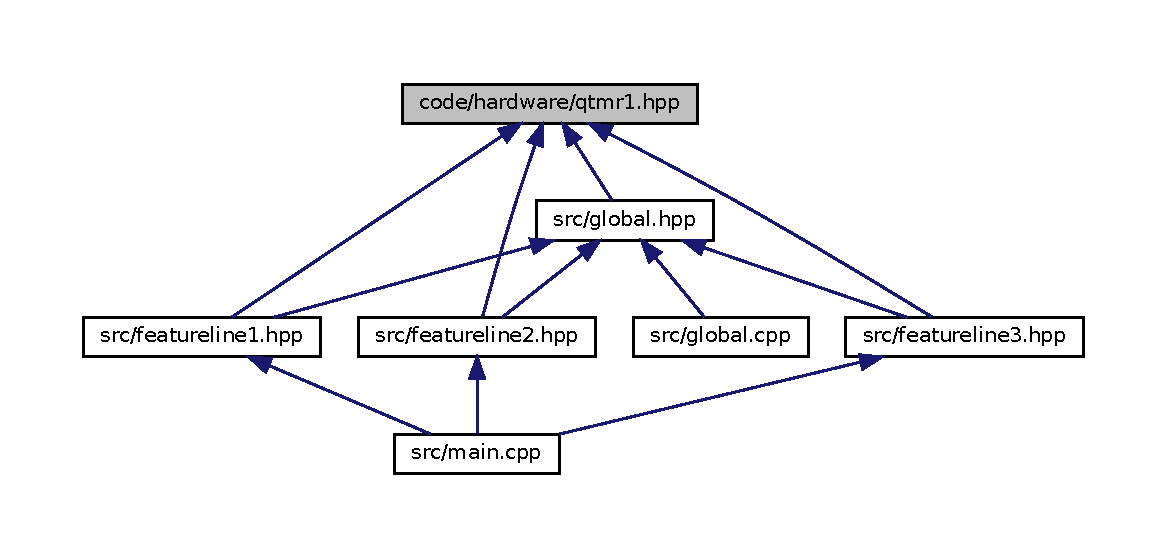
\includegraphics[width=350pt]{de/dea/qtmr1_8hpp__dep__incl}
\end{center}
\end{figure}
\subsection*{Classes}
\begin{DoxyCompactItemize}
\item 
class \hyperlink{classTMR1Controller}{T\+M\+R1\+Controller}
\begin{DoxyCompactList}\small\item\em Templated interface for Quad Timer 1 channels for Gate Counting. The module uses the macro {\ttfamily \+\_\+\+T\+M\+R1\+\_\+\+C\+O\+N\+T\+R\+O\+L\+L\+E\+R\+\_\+\+C\+H\+\_\+} to identify the main channel and then assigns the next channel\textquotesingle{}s ({\itshape T\+M\+R1\+\_\+\+C\+O\+N\+T\+R\+O\+L\+L\+E\+R\+\_\+\+CH} + 1) external pin to the {\itshape T\+M\+R1\+\_\+\+C\+O\+N\+T\+R\+O\+L\+L\+E\+R\+\_\+\+CH} as the \char`\"{}\+Capture Pin\char`\"{} or the \char`\"{}\+Secondary Count Source\char`\"{}. \end{DoxyCompactList}\end{DoxyCompactItemize}
\subsection*{Macros}
\begin{DoxyCompactItemize}
\item 
\#define \hyperlink{qtmr1_8hpp_a9b1e0ba00a31105b8b486365043a4cd2}{\+\_\+\+T\+M\+R1\+\_\+\+C\+O\+N\+T\+R\+O\+L\+L\+E\+R\+\_\+\+C\+H\+\_\+}~0
\end{DoxyCompactItemize}


\subsection{Macro Definition Documentation}
\mbox{\Hypertarget{qtmr1_8hpp_a9b1e0ba00a31105b8b486365043a4cd2}\label{qtmr1_8hpp_a9b1e0ba00a31105b8b486365043a4cd2}} 
\index{qtmr1.\+hpp@{qtmr1.\+hpp}!\+\_\+\+T\+M\+R1\+\_\+\+C\+O\+N\+T\+R\+O\+L\+L\+E\+R\+\_\+\+C\+H\+\_\+@{\+\_\+\+T\+M\+R1\+\_\+\+C\+O\+N\+T\+R\+O\+L\+L\+E\+R\+\_\+\+C\+H\+\_\+}}
\index{\+\_\+\+T\+M\+R1\+\_\+\+C\+O\+N\+T\+R\+O\+L\+L\+E\+R\+\_\+\+C\+H\+\_\+@{\+\_\+\+T\+M\+R1\+\_\+\+C\+O\+N\+T\+R\+O\+L\+L\+E\+R\+\_\+\+C\+H\+\_\+}!qtmr1.\+hpp@{qtmr1.\+hpp}}
\subsubsection{\texorpdfstring{\+\_\+\+T\+M\+R1\+\_\+\+C\+O\+N\+T\+R\+O\+L\+L\+E\+R\+\_\+\+C\+H\+\_\+}{\_TMR1\_CONTROLLER\_CH\_}}
{\footnotesize\ttfamily \#define \+\_\+\+T\+M\+R1\+\_\+\+C\+O\+N\+T\+R\+O\+L\+L\+E\+R\+\_\+\+C\+H\+\_\+~0}


\hypertarget{utilities_8hpp}{}\section{code/hardware/utilities.hpp File Reference}
\label{utilities_8hpp}\index{code/hardware/utilities.\+hpp@{code/hardware/utilities.\+hpp}}
{\ttfamily \#include $<$imxrt.\+h$>$}\newline
Include dependency graph for utilities.\+hpp\+:\nopagebreak
\begin{figure}[H]
\begin{center}
\leavevmode
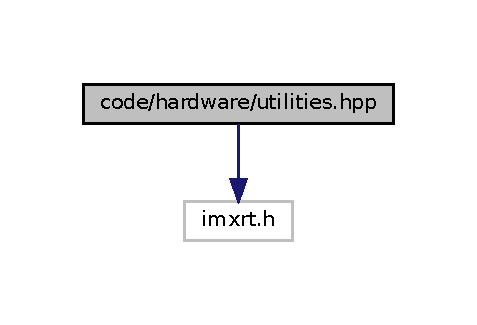
\includegraphics[width=229pt]{df/d46/utilities_8hpp__incl}
\end{center}
\end{figure}
This graph shows which files directly or indirectly include this file\+:
\nopagebreak
\begin{figure}[H]
\begin{center}
\leavevmode
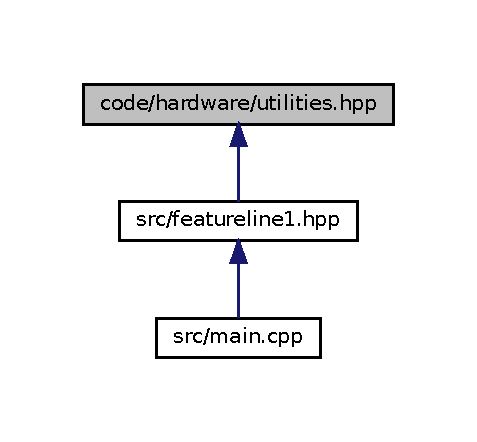
\includegraphics[width=229pt]{db/d84/utilities_8hpp__dep__incl}
\end{center}
\end{figure}
\subsection*{Macros}
\begin{DoxyCompactItemize}
\item 
\#define \hyperlink{utilities_8hpp_a4063879653b587261fa428e2a9d662b4}{P\+R\+R\+EG}(x)~Serial.\+print(\#x\char`\"{} 0x\char`\"{}); Serial.\+println(x,\+H\+E\+X)
\end{DoxyCompactItemize}
\subsection*{Functions}
\begin{DoxyCompactItemize}
\item 
void \hyperlink{utilities_8hpp_aceb15fdf783b1e9be1ef0d0fff5b5907}{xbar\+\_\+connect} (unsigned int input, unsigned int output)
\begin{DoxyCompactList}\small\item\em Establishes connection over X\+B\+A\+R1-\/A, given the input and output xbar pins  -\/ \href{https://github.com/manitou48/teensy4/blob/bc8fc46af5065a3f84352e0474069ae7a1a13064/pitxbaradc.ino#L40}{\tt https\+://github.\+com/manitou48/teensy4/blob/bc8fc46af5065a3f84352e0474069ae7a1a13064/pitxbaradc.\+ino\#\+L40}  -\/ Not specified. \end{DoxyCompactList}\item 
uint32\+\_\+t \hyperlink{utilities_8hpp_a1fb00a623d8b292185132f57935148a9}{F\+\_\+\+C\+P\+U\+\_\+tick\+\_\+count} ()
\item 
float \hyperlink{utilities_8hpp_a126c38ddf2ada96665a56b590a631776}{get\+\_\+\+C\+P\+U\+\_\+temp} ()
\end{DoxyCompactItemize}


\subsection{Macro Definition Documentation}
\mbox{\Hypertarget{utilities_8hpp_a4063879653b587261fa428e2a9d662b4}\label{utilities_8hpp_a4063879653b587261fa428e2a9d662b4}} 
\index{utilities.\+hpp@{utilities.\+hpp}!P\+R\+R\+EG@{P\+R\+R\+EG}}
\index{P\+R\+R\+EG@{P\+R\+R\+EG}!utilities.\+hpp@{utilities.\+hpp}}
\subsubsection{\texorpdfstring{P\+R\+R\+EG}{PRREG}}
{\footnotesize\ttfamily \#define P\+R\+R\+EG(\begin{DoxyParamCaption}\item[{}]{x }\end{DoxyParamCaption})~Serial.\+print(\#x\char`\"{} 0x\char`\"{}); Serial.\+println(x,\+H\+E\+X)}



\subsection{Function Documentation}
\mbox{\Hypertarget{utilities_8hpp_a1fb00a623d8b292185132f57935148a9}\label{utilities_8hpp_a1fb00a623d8b292185132f57935148a9}} 
\index{utilities.\+hpp@{utilities.\+hpp}!F\+\_\+\+C\+P\+U\+\_\+tick\+\_\+count@{F\+\_\+\+C\+P\+U\+\_\+tick\+\_\+count}}
\index{F\+\_\+\+C\+P\+U\+\_\+tick\+\_\+count@{F\+\_\+\+C\+P\+U\+\_\+tick\+\_\+count}!utilities.\+hpp@{utilities.\+hpp}}
\subsubsection{\texorpdfstring{F\+\_\+\+C\+P\+U\+\_\+tick\+\_\+count()}{F\_CPU\_tick\_count()}}
{\footnotesize\ttfamily uint32\+\_\+t F\+\_\+\+C\+P\+U\+\_\+tick\+\_\+count (\begin{DoxyParamCaption}{ }\end{DoxyParamCaption})}

\mbox{\Hypertarget{utilities_8hpp_a126c38ddf2ada96665a56b590a631776}\label{utilities_8hpp_a126c38ddf2ada96665a56b590a631776}} 
\index{utilities.\+hpp@{utilities.\+hpp}!get\+\_\+\+C\+P\+U\+\_\+temp@{get\+\_\+\+C\+P\+U\+\_\+temp}}
\index{get\+\_\+\+C\+P\+U\+\_\+temp@{get\+\_\+\+C\+P\+U\+\_\+temp}!utilities.\+hpp@{utilities.\+hpp}}
\subsubsection{\texorpdfstring{get\+\_\+\+C\+P\+U\+\_\+temp()}{get\_CPU\_temp()}}
{\footnotesize\ttfamily float get\+\_\+\+C\+P\+U\+\_\+temp (\begin{DoxyParamCaption}{ }\end{DoxyParamCaption})}

\mbox{\Hypertarget{utilities_8hpp_aceb15fdf783b1e9be1ef0d0fff5b5907}\label{utilities_8hpp_aceb15fdf783b1e9be1ef0d0fff5b5907}} 
\index{utilities.\+hpp@{utilities.\+hpp}!xbar\+\_\+connect@{xbar\+\_\+connect}}
\index{xbar\+\_\+connect@{xbar\+\_\+connect}!utilities.\+hpp@{utilities.\+hpp}}
\subsubsection{\texorpdfstring{xbar\+\_\+connect()}{xbar\_connect()}}
{\footnotesize\ttfamily void xbar\+\_\+connect (\begin{DoxyParamCaption}\item[{unsigned int}]{input,  }\item[{unsigned int}]{output }\end{DoxyParamCaption})}



Establishes connection over X\+B\+A\+R1-\/A, given the input and output xbar pins  -\/ \href{https://github.com/manitou48/teensy4/blob/bc8fc46af5065a3f84352e0474069ae7a1a13064/pitxbaradc.ino#L40}{\tt https\+://github.\+com/manitou48/teensy4/blob/bc8fc46af5065a3f84352e0474069ae7a1a13064/pitxbaradc.\+ino\#\+L40}  -\/ Not specified. 


\hypertarget{config_8py}{}\section{code/python/config.py File Reference}
\label{config_8py}\index{code/python/config.\+py@{code/python/config.\+py}}
\subsection*{Namespaces}
\begin{DoxyCompactItemize}
\item 
 \hyperlink{namespaceconfig}{config}
\end{DoxyCompactItemize}
\subsection*{Functions}
\begin{DoxyCompactItemize}
\item 
def \hyperlink{namespaceconfig_a8e5e09166a67c11eb868143f4e85607f}{config.\+generate\+\_\+config\+\_\+file} ()
\item 
def \hyperlink{namespaceconfig_ab97d69eb9e4097d1e43e248b73676d6a}{config.\+validate\+\_\+config\+\_\+file} (config\+\_\+file)
\end{DoxyCompactItemize}
\subsection*{Variables}
\begin{DoxyCompactItemize}
\item 
dictionary \hyperlink{namespaceconfig_ac321195dcb6ced179a85db093e63a1c9}{config.\+default\+\_\+config}
\end{DoxyCompactItemize}

\hypertarget{device__mode_8py}{}\section{code/pc\+\_\+app/device\+\_\+mode.py File Reference}
\label{device__mode_8py}\index{code/pc\+\_\+app/device\+\_\+mode.\+py@{code/pc\+\_\+app/device\+\_\+mode.\+py}}
\subsection*{Classes}
\begin{DoxyCompactItemize}
\item 
class \hyperlink{classdevice__mode_1_1StructParsar}{device\+\_\+mode.\+Struct\+Parsar}
\item 
class \hyperlink{classdevice__mode_1_1DataStore}{device\+\_\+mode.\+Data\+Store}
\item 
class \hyperlink{classdevice__mode_1_1FeatureLine}{device\+\_\+mode.\+Feature\+Line}
\end{DoxyCompactItemize}
\subsection*{Namespaces}
\begin{DoxyCompactItemize}
\item 
 \hyperlink{namespacedevice__mode}{device\+\_\+mode}
\end{DoxyCompactItemize}

\hypertarget{live__graph_8py}{}\section{code/pc\+\_\+app/live\+\_\+graph.py File Reference}
\label{live__graph_8py}\index{code/pc\+\_\+app/live\+\_\+graph.\+py@{code/pc\+\_\+app/live\+\_\+graph.\+py}}
\subsection*{Classes}
\begin{DoxyCompactItemize}
\item 
class \hyperlink{classlive__graph_1_1PStatLiveGraph}{live\+\_\+graph.\+P\+Stat\+Live\+Graph}
\end{DoxyCompactItemize}
\subsection*{Namespaces}
\begin{DoxyCompactItemize}
\item 
 \hyperlink{namespacelive__graph}{live\+\_\+graph}
\end{DoxyCompactItemize}

\hypertarget{livegraph_8py}{}\section{code/pc\+\_\+app/livegraph.py File Reference}
\label{livegraph_8py}\index{code/pc\+\_\+app/livegraph.\+py@{code/pc\+\_\+app/livegraph.\+py}}
\subsection*{Namespaces}
\begin{DoxyCompactItemize}
\item 
 \hyperlink{namespacelivegraph}{livegraph}
\end{DoxyCompactItemize}
\subsection*{Functions}
\begin{DoxyCompactItemize}
\item 
def \hyperlink{namespacelivegraph_aee36bd101e4ca90cf4635c2c7f3da10e}{livegraph.\+Live\+Graph} (x\+Range=None, y\+Range=None, kwargs)
\end{DoxyCompactItemize}

\hypertarget{multitau_8py}{}\section{code/pc\+\_\+app/multitau.py File Reference}
\label{multitau_8py}\index{code/pc\+\_\+app/multitau.\+py@{code/pc\+\_\+app/multitau.\+py}}
\subsection*{Namespaces}
\begin{DoxyCompactItemize}
\item 
 \hyperlink{namespacemultitau}{multitau}
\end{DoxyCompactItemize}
\subsection*{Functions}
\begin{DoxyCompactItemize}
\item 
def \hyperlink{namespacemultitau_a1022c52950a892396ac45e7de5379e12}{multitau.\+channel\+\_\+size} (lin\+\_\+corrs, series\+\_\+size, bin\+\_\+ratio)
\item 
def \hyperlink{namespacemultitau_a775aea685fe55a6707400660fadf9c35}{multitau.\+x\+\_\+tics} (lin\+\_\+corrs, series\+\_\+size, bin\+\_\+ratio)
\item 
def \hyperlink{namespacemultitau_a265372a8ef814094424e2d787eb6304f}{multitau.\+points\+\_\+scale\+\_\+template} (lin\+\_\+corrs, series\+\_\+size, bin\+\_\+ratio)
\item 
def \hyperlink{namespacemultitau_a40d600d74abad18e71cccd90988a5cd7}{multitau.\+bin\+\_\+ratio\+\_\+scale} (lin\+\_\+corrs, series\+\_\+size, bin\+\_\+ratio)
\item 
def \hyperlink{namespacemultitau_a9516fc9217f79f4dc1c4f2dfb28c9b7a}{multitau.\+tau\+\_\+max} (lin\+\_\+corrs, series\+\_\+size, bin\+\_\+ratio)
\item 
def \hyperlink{namespacemultitau_aa907c1cffb653422b45f46332192b2a4}{multitau.\+time\+\_\+axis\+\_\+s} (tau\+\_\+axis, gate\+\_\+time\+\_\+ms)
\item 
def \hyperlink{namespacemultitau_a89bb2627a88498b04ebd436250310d71}{multitau.\+points\+\_\+norm} (lin\+\_\+corrs, series\+\_\+size, bin\+\_\+ratio, L\+C0\+\_\+points)
\end{DoxyCompactItemize}

\hypertarget{new__app_8py}{}\section{code/pc\+\_\+app/new\+\_\+app.py File Reference}
\label{new__app_8py}\index{code/pc\+\_\+app/new\+\_\+app.\+py@{code/pc\+\_\+app/new\+\_\+app.\+py}}
\subsection*{Classes}
\begin{DoxyCompactItemize}
\item 
class \hyperlink{classnew__app_1_1ParamStruct}{new\+\_\+app.\+Param\+Struct}
\end{DoxyCompactItemize}
\subsection*{Namespaces}
\begin{DoxyCompactItemize}
\item 
 \hyperlink{namespacenew__app}{new\+\_\+app}
\end{DoxyCompactItemize}
\subsection*{Functions}
\begin{DoxyCompactItemize}
\item 
def \hyperlink{namespacenew__app_a3861515cd807c9fe679ffb2c2ac7e208}{new\+\_\+app.\+update\+\_\+fn} ()
\end{DoxyCompactItemize}
\subsection*{Variables}
\begin{DoxyCompactItemize}
\item 
\hyperlink{namespacenew__app_a18f2d0f3bfc48f8054be097380e3e91f}{new\+\_\+app.\+stop\+\_\+code\+\_\+asserted}
\end{DoxyCompactItemize}

\hypertarget{normalizer_8py}{}\section{code/pc\+\_\+app/normalizer.py File Reference}
\label{normalizer_8py}\index{code/pc\+\_\+app/normalizer.\+py@{code/pc\+\_\+app/normalizer.\+py}}
\subsection*{Classes}
\begin{DoxyCompactItemize}
\item 
class \hyperlink{classnormalizer_1_1Normalizer}{normalizer.\+Normalizer}
\end{DoxyCompactItemize}
\subsection*{Namespaces}
\begin{DoxyCompactItemize}
\item 
 \hyperlink{namespacenormalizer}{normalizer}
\end{DoxyCompactItemize}

\hypertarget{photon__statistics_8py}{}\section{code/pc\+\_\+app/photon\+\_\+statistics.py File Reference}
\label{photon__statistics_8py}\index{code/pc\+\_\+app/photon\+\_\+statistics.\+py@{code/pc\+\_\+app/photon\+\_\+statistics.\+py}}
\subsection*{Namespaces}
\begin{DoxyCompactItemize}
\item 
 \hyperlink{namespacephoton__statistics}{photon\+\_\+statistics}
\end{DoxyCompactItemize}
\subsection*{Functions}
\begin{DoxyCompactItemize}
\item 
def \hyperlink{namespacephoton__statistics_ad67c22ae3d8b73d690282b77915fa984}{photon\+\_\+statistics.\+update\+\_\+fn} ()
\item 
def \hyperlink{namespacephoton__statistics_a3d8a4bcc1566dd71aab0925749e1416f}{photon\+\_\+statistics.\+periodic\+\_\+callback\+\_\+fn} (period\+\_\+ms=measurement\+\_\+sampling\+\_\+delay)
\end{DoxyCompactItemize}
\subsection*{Variables}
\begin{DoxyCompactItemize}
\item 
\hyperlink{namespacephoton__statistics_a729c361165a662402f88b585477d2ee6}{photon\+\_\+statistics.\+name\+\_\+} = sys.\+argv\mbox{[}1\mbox{]}
\item 
\hyperlink{namespacephoton__statistics_a4176c548148b1c86da6ddf320ab00e90}{photon\+\_\+statistics.\+config} = json.\+load(f)
\item 
list \hyperlink{namespacephoton__statistics_a3c57d728c4b1cdcb2b6ca63bc6adfc4d}{photon\+\_\+statistics.\+multitau\+\_\+param\+\_\+set} = \mbox{[}config\mbox{[}\textquotesingle{}MT Linear Correlators(L\+Cs)\textquotesingle{}\mbox{]}, config\mbox{[}\textquotesingle{}MT LC Series Size\textquotesingle{}\mbox{]}, config\mbox{[}\textquotesingle{}MT Bin Ratio\textquotesingle{}\mbox{]}\mbox{]}
\item 
\hyperlink{namespacephoton__statistics_a397f80b778ada9e9d514e3ed06936540}{photon\+\_\+statistics.\+this\+\_\+channel\+\_\+size} = \hyperlink{namespacemultitau_a1022c52950a892396ac45e7de5379e12}{multitau.\+channel\+\_\+size}($\ast$multitau\+\_\+param\+\_\+set)
\item 
int \hyperlink{namespacephoton__statistics_a12cca295f67eb3583c567d9907a3fe4f}{photon\+\_\+statistics.\+byte\+\_\+size} = 4
\item 
tuple \hyperlink{namespacephoton__statistics_aa8b4fc62029e126fa660593daaa282f8}{photon\+\_\+statistics.\+total\+\_\+struct\+\_\+size}
\item 
bool \hyperlink{namespacephoton__statistics_ae06425daaa0688ab0ff42c7619615e1d}{photon\+\_\+statistics.\+stop\+\_\+code\+\_\+asserted} = False
\item 
int \hyperlink{namespacephoton__statistics_aa0ea01ea8f5c4844ed6c10dbe51d0497}{photon\+\_\+statistics.\+update\+\_\+id} = 0
\item 
list \hyperlink{namespacephoton__statistics_ad632a8023bd406f2a2486a1c5d3e7832}{photon\+\_\+statistics.\+openfilelist} = \mbox{[}$\,$\mbox{]}
\item 
string \hyperlink{namespacephoton__statistics_a255f06b87745f05837e1623b921ae692}{photon\+\_\+statistics.\+parent\+\_\+dir} = \char`\"{}./runs/\char`\"{}
\item 
string \hyperlink{namespacephoton__statistics_ab381c3496e1a3a8d6dae99e66447c10c}{photon\+\_\+statistics.\+D\+A\+T\+A\+S\+EP} = \textquotesingle{},\textquotesingle{}
\item 
\hyperlink{namespacephoton__statistics_a421423fcce411e182e41fde2e450d2d9}{photon\+\_\+statistics.\+now\+\_\+tmp} = time.\+perf\+\_\+counter()
\item 
\hyperlink{namespacephoton__statistics_a2c4e09ca6009ec89417e7fb1842dc290}{photon\+\_\+statistics.\+update\+\_\+time\+\_\+start} = now\+\_\+tmp
\item 
\hyperlink{namespacephoton__statistics_a1353da1c17a4f960cbacf200dcf13d4f}{photon\+\_\+statistics.\+update\+\_\+time\+\_\+stop} = now\+\_\+tmp
\item 
\hyperlink{namespacephoton__statistics_a5c7400e3258e9336ce831f0fbda24f33}{photon\+\_\+statistics.\+measure\+\_\+clock\+\_\+start} = now\+\_\+tmp
\item 
\hyperlink{namespacephoton__statistics_a328243354a643086bd68145d804782d0}{photon\+\_\+statistics.\+measure\+\_\+clock\+\_\+stop} = now\+\_\+tmp
\item 
\hyperlink{namespacephoton__statistics_a930bc99eb656180a9ae6318b16d77976}{photon\+\_\+statistics.\+x\+\_\+tau\+\_\+values} = \hyperlink{namespacemultitau_a775aea685fe55a6707400660fadf9c35}{multitau.\+x\+\_\+tics}($\ast$multitau\+\_\+param\+\_\+set)
\item 
\hyperlink{namespacephoton__statistics_a4476861cf199e5ef481ee4bc15e08847}{photon\+\_\+statistics.\+normalizer} = Normalizer($\ast$multitau\+\_\+param\+\_\+set)
\item 
tuple \hyperlink{namespacephoton__statistics_a28a89caae4538b504046ed301158e677}{photon\+\_\+statistics.\+norm\+\_\+mode} = (\char`\"{}no\char`\"{} $\ast$ (not config\mbox{[}\char`\"{}Enable Points Norm\char`\"{}\mbox{]})) + (\char`\"{}points\char`\"{} $\ast$ (not config\mbox{[}\char`\"{}Enable Mean Norm\char`\"{}\mbox{]}) $\ast$ config\mbox{[}\char`\"{}Enable Points Norm\char`\"{}\mbox{]}) + (\char`\"{}mean\char`\"{} $\ast$ config\mbox{[}\char`\"{}Enable Mean Norm\char`\"{}\mbox{]} $\ast$ config\mbox{[}\char`\"{}Enable Points Norm\char`\"{}\mbox{]})
\item 
list \hyperlink{namespacephoton__statistics_af558fed5a93a7b134efea382f1ad4007}{photon\+\_\+statistics.\+norm\+\_\+args} = \mbox{[}$\,$\mbox{]}
\item 
\hyperlink{namespacephoton__statistics_a1a182b084119bc408c9fbae7b462acc3}{photon\+\_\+statistics.\+struct\+\_\+rep} = Struct\+Representation(config)
\item 
\hyperlink{namespacephoton__statistics_a718548ec119098f106f9ff9f31b409bf}{photon\+\_\+statistics.\+time\+\_\+x} = deque(maxlen = 100)
\item 
\hyperlink{namespacephoton__statistics_a9939968ed5be4ad1c5c6264ed0a875e9}{photon\+\_\+statistics.\+count\+\_\+rate\+\_\+y} = deque(maxlen = 100)
\item 
\hyperlink{namespacephoton__statistics_a5394aea076650f9894b4cb28977546d5}{photon\+\_\+statistics.\+mean\+\_\+int\+\_\+y} = deque(maxlen = 100)
\item 
\hyperlink{namespacephoton__statistics_a397e27175ec763175de0a4b04e9beb75}{photon\+\_\+statistics.\+pf\+\_\+serial\+\_\+y} = deque(maxlen = 100)
\item 
\hyperlink{namespacephoton__statistics_ada08824fb72ac8fb00ca57eb5ffa0a59}{photon\+\_\+statistics.\+pf\+\_\+acf\+\_\+y} = deque(maxlen = 100)
\item 
string \hyperlink{namespacephoton__statistics_af562d689a2b300926d155fb601e925ae}{photon\+\_\+statistics.\+y\+\_\+file\+\_\+name} = f\char`\"{}\{name\+\_\+\}\+\_\+y.\+dat\char`\"{}
\item 
string \hyperlink{namespacephoton__statistics_ac46f5d89cfe3237a86a586214643616d}{photon\+\_\+statistics.\+x\+\_\+file\+\_\+name} = f\char`\"{}\{name\+\_\+\}\+\_\+x\+\_\+taus.\+dat\char`\"{}
\item 
\hyperlink{namespacephoton__statistics_a0e1aee8b528dd37bb27185509aa5af09}{photon\+\_\+statistics.\+fmt}
\item 
\hyperlink{namespacephoton__statistics_a6c6d01b62f113634193642d2dda3124a}{photon\+\_\+statistics.\+newline}
\item 
\hyperlink{namespacephoton__statistics_ad37c8420c6a43ec4997809c4c236b145}{photon\+\_\+statistics.\+acffile} = open(os.\+path.\+join(parent\+\_\+dir, y\+\_\+file\+\_\+name), \textquotesingle{}a\textquotesingle{})
\item 
string \hyperlink{namespacephoton__statistics_aefac3a6449e578f00a5870a4249bf7ea}{photon\+\_\+statistics.\+count\+\_\+file\+\_\+name} = f\char`\"{}\{name\+\_\+\}\+\_\+countrate.\+dat\char`\"{}
\item 
\hyperlink{namespacephoton__statistics_af015eefc8f4b272cae12b376618be9dc}{photon\+\_\+statistics.\+countratefile} = open(os.\+path.\+join(parent\+\_\+dir, count\+\_\+file\+\_\+name), \textquotesingle{}w\textquotesingle{})
\item 
string \hyperlink{namespacephoton__statistics_a86328a634773cdedebc0fd4be6a8a068}{photon\+\_\+statistics.\+mean\+\_\+file\+\_\+name} = f\char`\"{}\{name\+\_\+\}\+\_\+meanintensity.\+dat\char`\"{}
\item 
\hyperlink{namespacephoton__statistics_a39901f127e13a9b2adb1e3624e51cdc9}{photon\+\_\+statistics.\+meanfile} = open(os.\+path.\+join(parent\+\_\+dir, mean\+\_\+file\+\_\+name), \textquotesingle{}w\textquotesingle{})
\item 
\hyperlink{namespacephoton__statistics_a75ad62bb71f891a32137fe2fd41d40d9}{photon\+\_\+statistics.\+live\+\_\+graph} = Live\+Graph(x\+Range=x\+\_\+tau\+\_\+values\mbox{[}-\/1\mbox{]}, port=config\mbox{[}\textquotesingle{}Port\textquotesingle{}\mbox{]}, title=\char`\"{}Auto-\/Correlation Function\char`\"{}, x\+\_\+label = \char`\"{}Lag\char`\"{}, y\+\_\+label=\char`\"{}A\+CF\char`\"{}, x\+\_\+units=\char`\"{}Tau\char`\"{}, y\+\_\+units=\char`\"{}G(Tau)\char`\"{}, config=config )
\item 
\hyperlink{namespacephoton__statistics_a76d9f47b30df749d7d370e77849ca649}{photon\+\_\+statistics.\+title}
\item 
\hyperlink{namespacephoton__statistics_a98d62096339004a1f6b233c2df89b3ba}{photon\+\_\+statistics.\+row}
\item 
\hyperlink{namespacephoton__statistics_a01b8c2da7bc3f1dd415a4c956cd2cd29}{photon\+\_\+statistics.\+col}
\item 
\hyperlink{namespacephoton__statistics_a01caa0fce4e95b6469fea2c15dec86b6}{photon\+\_\+statistics.\+rowspan}
\item 
\hyperlink{namespacephoton__statistics_a39fd907fbedfc2f81f1fdf9e6a29631a}{photon\+\_\+statistics.\+pen}
\item 
\hyperlink{namespacephoton__statistics_a5b8d0a21492531701eaab526f8d6ffda}{photon\+\_\+statistics.\+symbol\+Brush}
\item 
\hyperlink{namespacephoton__statistics_a31d8b2d681ba8e84148ca5a7a7d97829}{photon\+\_\+statistics.\+symbol\+Size}
\item 
\hyperlink{namespacephoton__statistics_a09fecae480663af684a1d523466242a4}{photon\+\_\+statistics.\+port} = Serial(port=config\mbox{[}\char`\"{}Port\char`\"{}\mbox{]}, baudrate=config\mbox{[}\char`\"{}Baud\char`\"{}\mbox{]}, timeout=None)
\item 
\hyperlink{namespacephoton__statistics_ab809da8a53764aea064814bd4abdba42}{photon\+\_\+statistics.\+measurement\+\_\+sampling\+\_\+delay} = int(config\mbox{[}\textquotesingle{}Sampling Delay ms\textquotesingle{}\mbox{]}/2)
\item 
\hyperlink{namespacephoton__statistics_a826b8bcc70f5721cbb6036088fa1ed01}{photon\+\_\+statistics.\+measurement\+\_\+thread} = Qt\+Core.\+Q\+Timer()
\item 
tuple \hyperlink{namespacephoton__statistics_a17e0852f9ef02250d5e11c55b45dcbf6}{photon\+\_\+statistics.\+received\+\_\+data\+\_\+estimate} = total\+\_\+struct\+\_\+size $\ast$ update\+\_\+id
\end{DoxyCompactItemize}

\hypertarget{statmethods_8py}{}\section{code/pc\+\_\+app/statmethods.py File Reference}
\label{statmethods_8py}\index{code/pc\+\_\+app/statmethods.\+py@{code/pc\+\_\+app/statmethods.\+py}}
\subsection*{Classes}
\begin{DoxyCompactItemize}
\item 
class \hyperlink{classstatmethods_1_1StatMethods}{statmethods.\+Stat\+Methods}
\end{DoxyCompactItemize}
\subsection*{Namespaces}
\begin{DoxyCompactItemize}
\item 
 \hyperlink{namespacestatmethods}{statmethods}
\end{DoxyCompactItemize}

\hypertarget{test_8py}{}\section{code/pc\+\_\+app/test.py File Reference}
\label{test_8py}\index{code/pc\+\_\+app/test.\+py@{code/pc\+\_\+app/test.\+py}}
\subsection*{Namespaces}
\begin{DoxyCompactItemize}
\item 
 \hyperlink{namespacetest}{test}
\end{DoxyCompactItemize}
\subsection*{Variables}
\begin{DoxyCompactItemize}
\item 
\hyperlink{namespacetest_accf9c2b29590b2e2d68bb2614364444e}{test.\+x} = np.\+load(\textquotesingle{}acf\+\_\+x.\+npy\textquotesingle{})
\item 
\hyperlink{namespacetest_a8e35cd41a1bbd5493b663b19c9df1d1d}{test.\+y} = np.\+load(\textquotesingle{}acf\+\_\+y.\+npy\textquotesingle{})
\item 
\hyperlink{namespacetest_a87d947ef7b0fcf728e1e7d6ec65c865f}{test.\+lg} = Live\+Graph(y\+Range=0.\+04)
\end{DoxyCompactItemize}

\hypertarget{utilities_8py}{}\section{code/pc\+\_\+app/utilities.py File Reference}
\label{utilities_8py}\index{code/pc\+\_\+app/utilities.\+py@{code/pc\+\_\+app/utilities.\+py}}
\subsection*{Namespaces}
\begin{DoxyCompactItemize}
\item 
 \hyperlink{namespaceutilities}{utilities}
\end{DoxyCompactItemize}
\subsection*{Functions}
\begin{DoxyCompactItemize}
\item 
def \hyperlink{namespaceutilities_a85150e8e264f76b149785770210a7f1a}{utilities.\+Pseudo\+Console} ()
\item 
def \hyperlink{namespaceutilities_a7c64a494f834c091373f2bb148dc2e8c}{utilities.\+Welcome\+Text} (name)
\item 
def \hyperlink{namespaceutilities_a35dce39ce5efc1ca1a29b30ffc373bd0}{utilities.\+periodic\+\_\+callbacks} (period\+\_\+ms, fn, args)
\item 
def \hyperlink{namespaceutilities_aa2added918da29f1fa28d3ea24d570d9}{utilities.\+Struct\+Representation} (config)
\end{DoxyCompactItemize}

\hypertarget{accumulator_8hpp}{}\section{lib/software/accumulator.hpp File Reference}
\label{accumulator_8hpp}\index{lib/software/accumulator.\+hpp@{lib/software/accumulator.\+hpp}}
{\ttfamily \#include \char`\"{}types.\+hpp\char`\"{}}\newline
{\ttfamily \#include \char`\"{}Lin\+\_\+\+A\+Corr\+\_\+\+R\+T\+\_\+\+Base.\+hpp\char`\"{}}\newline
Include dependency graph for accumulator.\+hpp\+:
\nopagebreak
\begin{figure}[H]
\begin{center}
\leavevmode
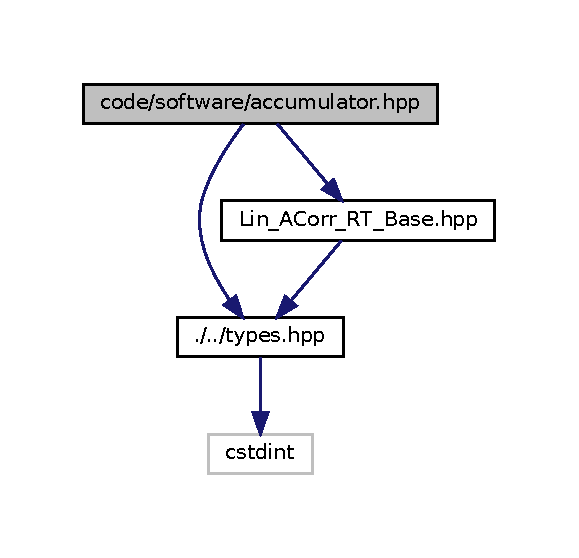
\includegraphics[width=272pt]{accumulator_8hpp__incl}
\end{center}
\end{figure}
This graph shows which files directly or indirectly include this file\+:
\nopagebreak
\begin{figure}[H]
\begin{center}
\leavevmode
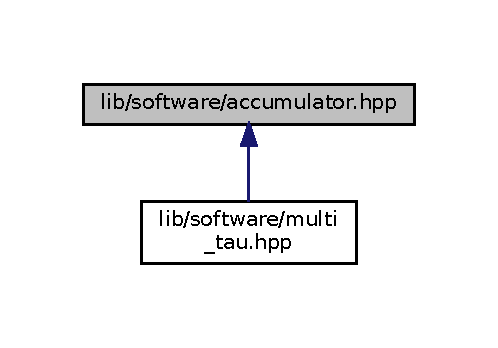
\includegraphics[width=239pt]{accumulator_8hpp__dep__incl}
\end{center}
\end{figure}
\subsection*{Classes}
\begin{DoxyCompactItemize}
\item 
class \hyperlink{classAccumulator}{Accumulator}
\begin{DoxyCompactList}\small\item\em Adapter object responsible for accumulating the points and coarsening the time-\/series as per the relavent linear-\/correlator time-\/resolution. \end{DoxyCompactList}\end{DoxyCompactItemize}

\hypertarget{discarder_8hpp}{}\section{/mnt/m/code/\+Correlator/\+Software/discarder.hpp File Reference}
\label{discarder_8hpp}\index{/mnt/m/code/\+Correlator/\+Software/discarder.\+hpp@{/mnt/m/code/\+Correlator/\+Software/discarder.\+hpp}}
{\ttfamily \#include \char`\"{}types.\+hpp\char`\"{}}\newline
{\ttfamily \#include \char`\"{}Lin\+\_\+\+A\+Corr\+\_\+\+R\+T\+\_\+\+Base.\+hpp\char`\"{}}\newline
Include dependency graph for discarder.\+hpp\+:
\nopagebreak
\begin{figure}[H]
\begin{center}
\leavevmode
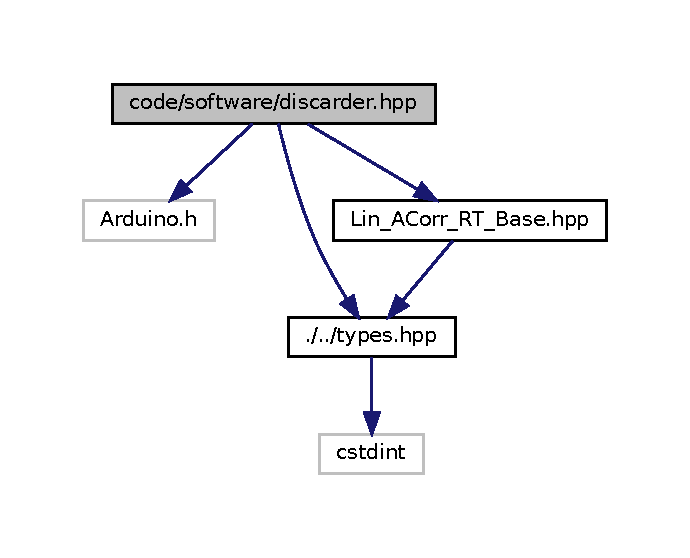
\includegraphics[width=259pt]{discarder_8hpp__incl}
\end{center}
\end{figure}
This graph shows which files directly or indirectly include this file\+:
\nopagebreak
\begin{figure}[H]
\begin{center}
\leavevmode
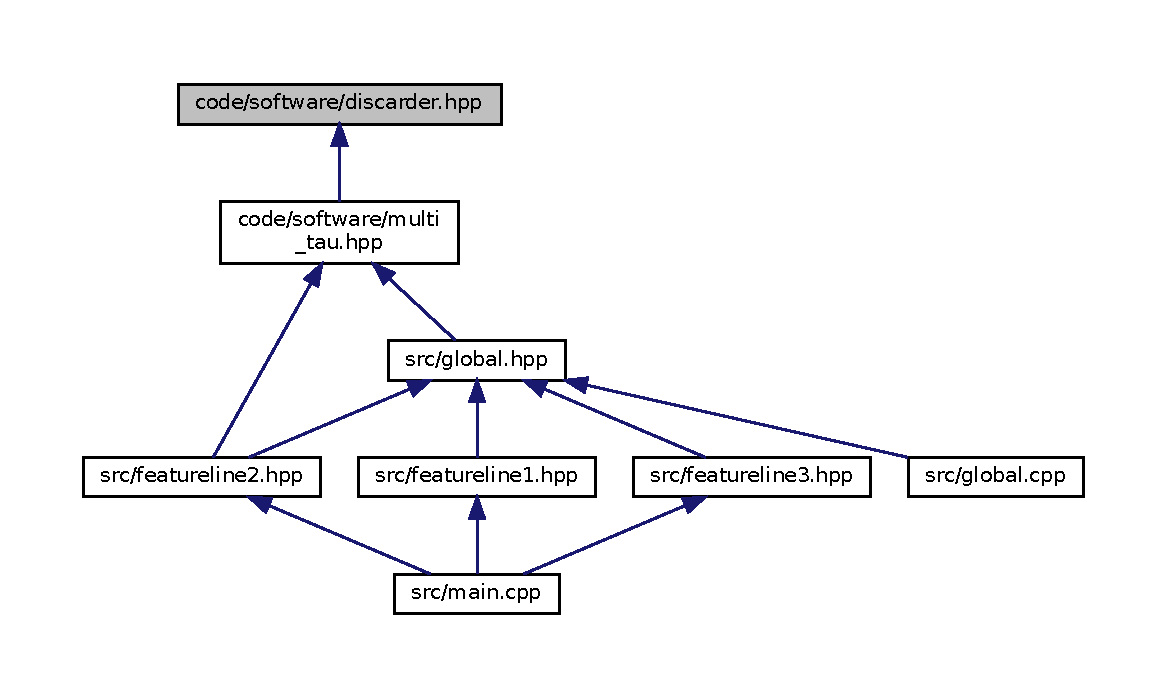
\includegraphics[width=214pt]{discarder_8hpp__dep__incl}
\end{center}
\end{figure}
\subsection*{Classes}
\begin{DoxyCompactItemize}
\item 
class \hyperlink{classFrontBack__Discarder__Base}{Front\+Back\+\_\+\+Discarder\+\_\+\+Base$<$ Series\+\_\+size, Front, End $>$}
\begin{DoxyCompactList}\small\item\em Base class for Front and Back discarder objects. \end{DoxyCompactList}\item 
class \hyperlink{classDiscarder__Teensy}{Discarder\+\_\+\+Teensy$<$ Series\+\_\+size, Front, End $>$}
\begin{DoxyCompactList}\small\item\em Teensy specific Front back discarder implementation. \end{DoxyCompactList}\end{DoxyCompactItemize}

\hypertarget{fakechannel_8hpp}{}\section{code/software/fakechannel.hpp File Reference}
\label{fakechannel_8hpp}\index{code/software/fakechannel.\+hpp@{code/software/fakechannel.\+hpp}}
{\ttfamily \#include \char`\"{}./../types.\+hpp\char`\"{}}\newline
{\ttfamily \#include \char`\"{}simpler\+\_\+circular\+\_\+buffer.\+hpp\char`\"{}}\newline
{\ttfamily \#include $<$Arduino.\+h$>$}\newline
Include dependency graph for fakechannel.\+hpp\+:
\nopagebreak
\begin{figure}[H]
\begin{center}
\leavevmode
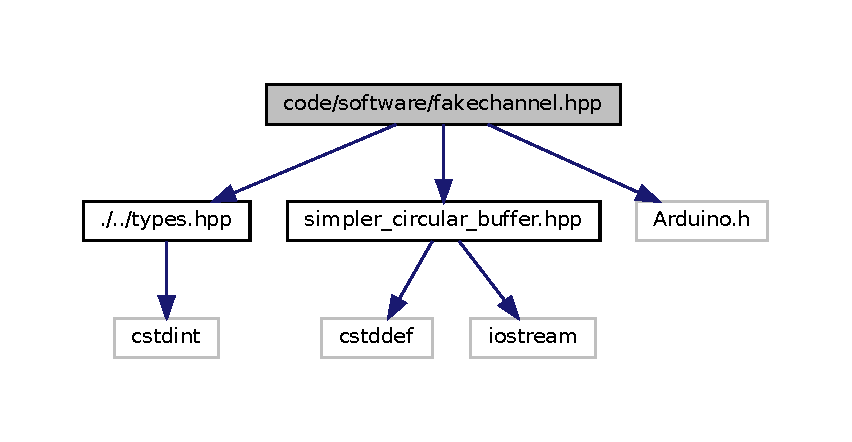
\includegraphics[width=350pt]{fakechannel_8hpp__incl}
\end{center}
\end{figure}
\subsection*{Classes}
\begin{DoxyCompactItemize}
\item 
class \hyperlink{classFakeChannel}{Fake\+Channel$<$ Series\+\_\+\+Size, has\+Monitor\+Channel $>$}
\begin{DoxyCompactList}\small\item\em This is an {\itshape duck typed} implementaion of a {\itshape Linear Correlator} that returns linearly increasing values for correlation. \end{DoxyCompactList}\end{DoxyCompactItemize}

\hypertarget{histogram_8hpp}{}\section{code/software/histogram.hpp File Reference}
\label{histogram_8hpp}\index{code/software/histogram.\+hpp@{code/software/histogram.\+hpp}}
{\ttfamily \#include $<$type\+\_\+traits$>$}\newline
{\ttfamily \#include \char`\"{}./../types.\+hpp\char`\"{}}\newline
{\ttfamily \#include $<$Arduino.\+h$>$}\newline
Include dependency graph for histogram.\+hpp\+:\nopagebreak
\begin{figure}[H]
\begin{center}
\leavevmode
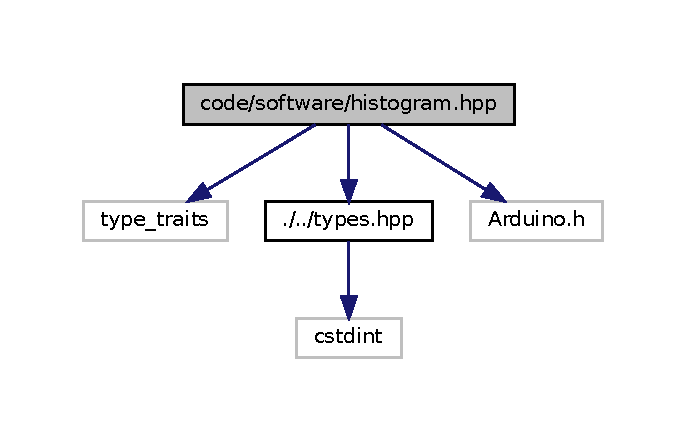
\includegraphics[width=329pt]{histogram_8hpp__incl}
\end{center}
\end{figure}
This graph shows which files directly or indirectly include this file\+:\nopagebreak
\begin{figure}[H]
\begin{center}
\leavevmode
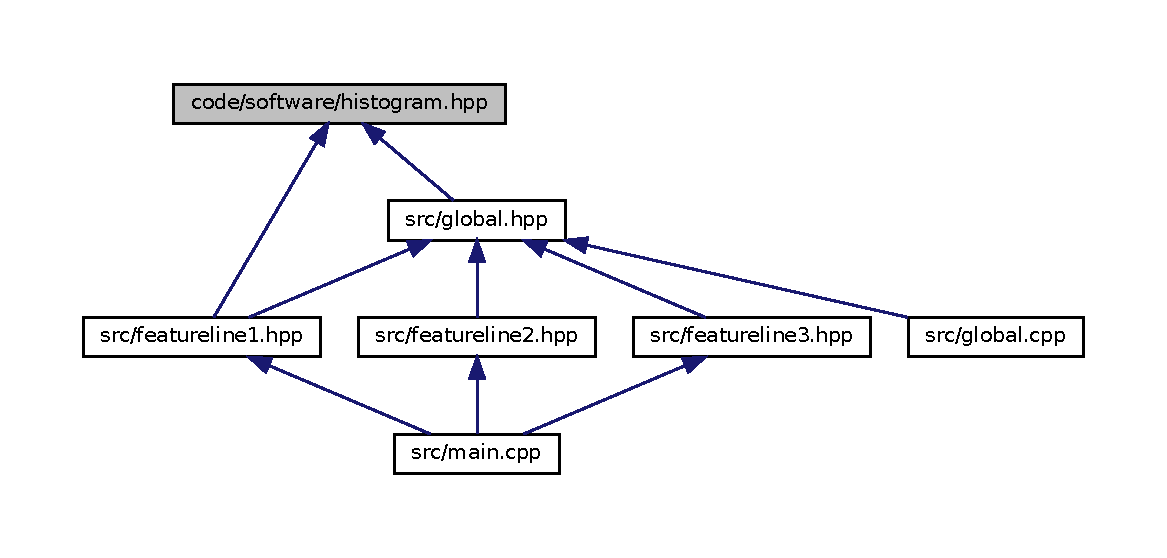
\includegraphics[width=350pt]{histogram_8hpp__dep__incl}
\end{center}
\end{figure}
\subsection*{Classes}
\begin{DoxyCompactItemize}
\item 
class \hyperlink{classPCHistogram}{P\+C\+Histogram$<$ Bin\+Type, Bins $>$}
\begin{DoxyCompactList}\small\item\em Photon Counting Histogram module for Real time calculation on {\itshape Teensy 4.\+1 microcontrollers}. \end{DoxyCompactList}\end{DoxyCompactItemize}

\hypertarget{Lin__ACorr__RT__Teensy_8hpp}{}\section{code/software/\+Lin\+\_\+\+A\+Corr\+\_\+\+R\+T\+\_\+\+Teensy.hpp File Reference}
\label{Lin__ACorr__RT__Teensy_8hpp}\index{code/software/\+Lin\+\_\+\+A\+Corr\+\_\+\+R\+T\+\_\+\+Teensy.\+hpp@{code/software/\+Lin\+\_\+\+A\+Corr\+\_\+\+R\+T\+\_\+\+Teensy.\+hpp}}
{\ttfamily \#include \char`\"{}./../types.\+hpp\char`\"{}}\newline
{\ttfamily \#include \char`\"{}simpler\+\_\+circular\+\_\+buffer.\+hpp\char`\"{}}\newline
{\ttfamily \#include $<$Arduino.\+h$>$}\newline
Include dependency graph for Lin\+\_\+\+A\+Corr\+\_\+\+R\+T\+\_\+\+Teensy.\+hpp\+:
\nopagebreak
\begin{figure}[H]
\begin{center}
\leavevmode
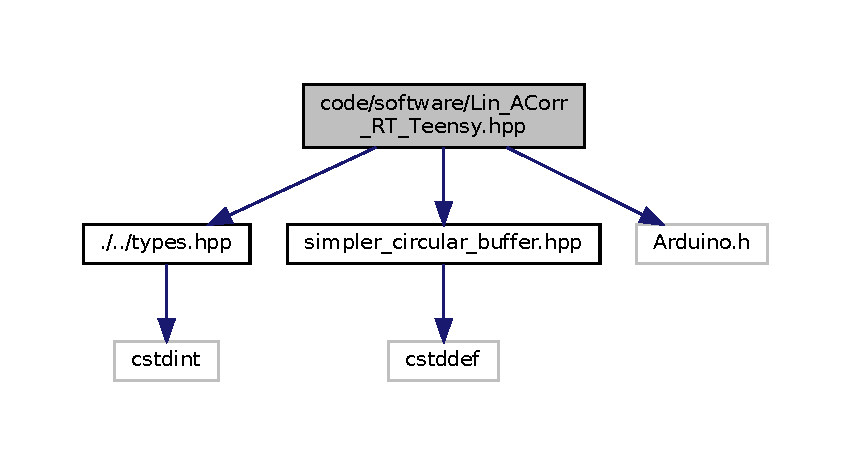
\includegraphics[width=350pt]{d5/d93/Lin__ACorr__RT__Teensy_8hpp__incl}
\end{center}
\end{figure}
This graph shows which files directly or indirectly include this file\+:
\nopagebreak
\begin{figure}[H]
\begin{center}
\leavevmode
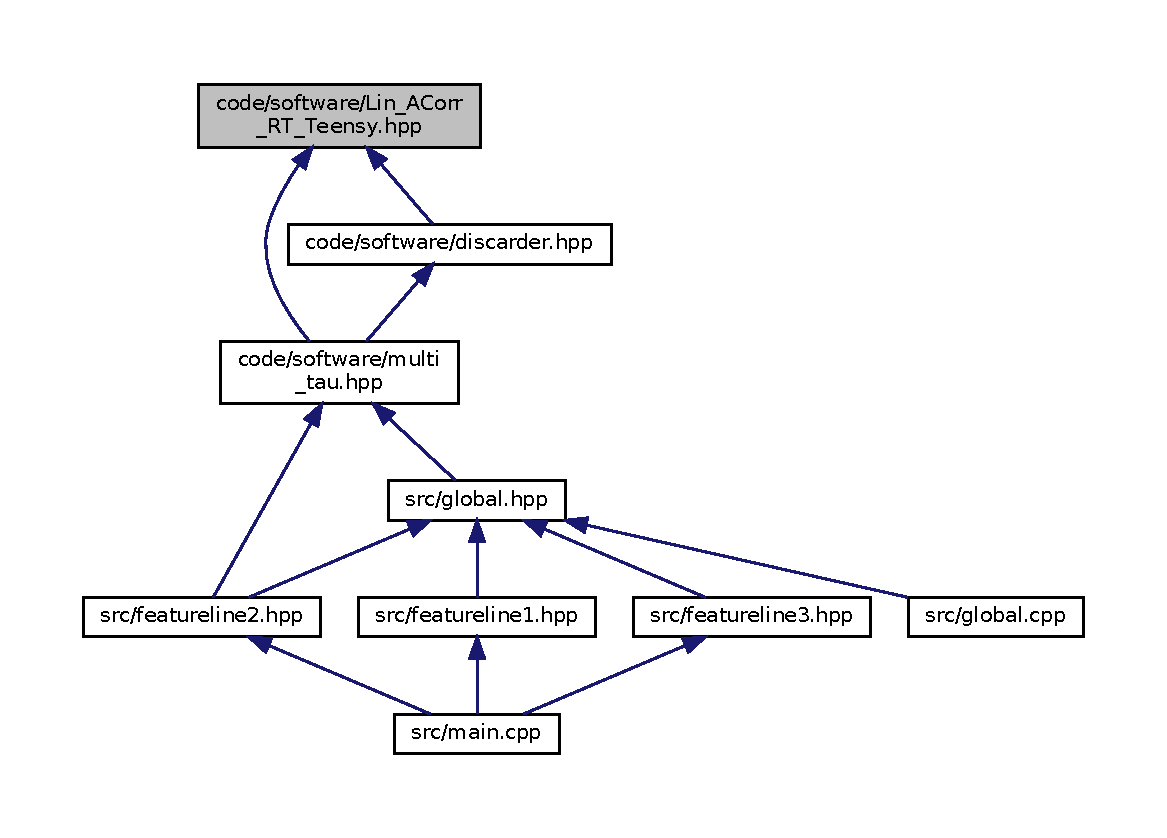
\includegraphics[width=350pt]{db/d9e/Lin__ACorr__RT__Teensy_8hpp__dep__incl}
\end{center}
\end{figure}
\subsection*{Classes}
\begin{DoxyCompactItemize}
\item 
class \hyperlink{classLinACorrRTTeensy}{Lin\+A\+Corr\+R\+T\+Teensy$<$ Series\+\_\+\+Size, has\+Monitor\+Channel $>$}
\begin{DoxyCompactList}\small\item\em This is an implementation of Lin\+\_\+\+A\+Corr\+\_\+\+R\+T\+\_\+\+Base for Teensy with {\bfseries }(No normalisation or baseline subtraction.) \end{DoxyCompactList}\end{DoxyCompactItemize}

\hypertarget{Lin__CrossCorr__RT__Teensy_8hpp}{}\section{code/software/\+Lin\+\_\+\+Cross\+Corr\+\_\+\+R\+T\+\_\+\+Teensy.hpp File Reference}
\label{Lin__CrossCorr__RT__Teensy_8hpp}\index{code/software/\+Lin\+\_\+\+Cross\+Corr\+\_\+\+R\+T\+\_\+\+Teensy.\+hpp@{code/software/\+Lin\+\_\+\+Cross\+Corr\+\_\+\+R\+T\+\_\+\+Teensy.\+hpp}}
{\ttfamily \#include \char`\"{}types.\+hpp\char`\"{}}\newline
{\ttfamily \#include \char`\"{}Lin\+\_\+\+Cross\+Corr\+\_\+\+R\+T\+\_\+\+Base.\+hpp\char`\"{}}\newline
Include dependency graph for Lin\+\_\+\+Cross\+Corr\+\_\+\+R\+T\+\_\+\+Teensy.\+hpp\+:
\nopagebreak
\begin{figure}[H]
\begin{center}
\leavevmode
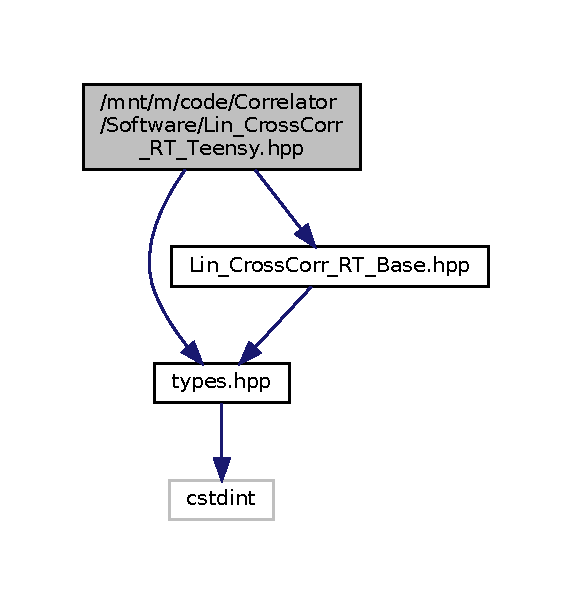
\includegraphics[width=286pt]{Lin__CrossCorr__RT__Teensy_8hpp__incl}
\end{center}
\end{figure}
\subsection*{Classes}
\begin{DoxyCompactItemize}
\item 
class \hyperlink{classLin__CrossCorr__RT__Teensy}{Lin\+\_\+\+Cross\+Corr\+\_\+\+R\+T\+\_\+\+Teensy$<$ Series\+\_\+size $>$}
\begin{DoxyCompactList}\small\item\em This is an implementation of \hyperlink{classLin__ACorr__RT__Base}{Lin\+\_\+\+A\+Corr\+\_\+\+R\+T\+\_\+\+Base} for Teensy with {\bfseries }(No normalisation or baseline subtraction.) \end{DoxyCompactList}\end{DoxyCompactItemize}

\hypertarget{monitor__channel_8hpp}{}\section{code/software/monitor\+\_\+channel.hpp File Reference}
\label{monitor__channel_8hpp}\index{code/software/monitor\+\_\+channel.\+hpp@{code/software/monitor\+\_\+channel.\+hpp}}
{\ttfamily \#include \char`\"{}./../types.\+hpp\char`\"{}}\newline
Include dependency graph for monitor\+\_\+channel.\+hpp\+:
\nopagebreak
\begin{figure}[H]
\begin{center}
\leavevmode
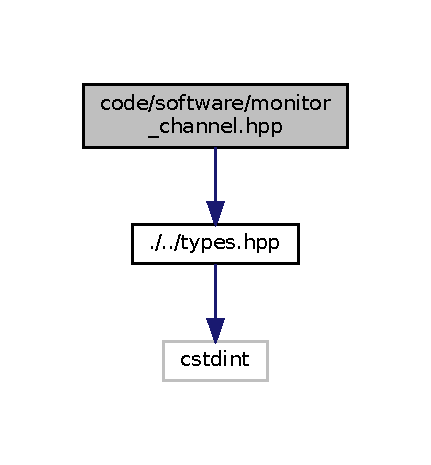
\includegraphics[width=207pt]{monitor__channel_8hpp__incl}
\end{center}
\end{figure}
\subsection*{Classes}
\begin{DoxyCompactItemize}
\item 
class \hyperlink{classMonitor__Channel}{Monitor\+\_\+\+Channel}
\begin{DoxyCompactList}\small\item\em A simple Averager Class that calculates the estimated mean. \end{DoxyCompactList}\end{DoxyCompactItemize}

\hypertarget{multi__tau_8hpp}{}\section{code/software/multi\+\_\+tau.hpp File Reference}
\label{multi__tau_8hpp}\index{code/software/multi\+\_\+tau.\+hpp@{code/software/multi\+\_\+tau.\+hpp}}
{\ttfamily \#include $<$cmath$>$}\newline
{\ttfamily \#include \char`\"{}./../types.\+hpp\char`\"{}}\newline
{\ttfamily \#include \char`\"{}Lin\+\_\+\+A\+Corr\+\_\+\+R\+T\+\_\+\+Teensy.\+hpp\char`\"{}}\newline
{\ttfamily \#include \char`\"{}accumulator.\+hpp\char`\"{}}\newline
{\ttfamily \#include \char`\"{}discarder.\+hpp\char`\"{}}\newline
{\ttfamily \#include \char`\"{}monitor\+\_\+channel.\+hpp\char`\"{}}\newline
Include dependency graph for multi\+\_\+tau.\+hpp\+:
\nopagebreak
\begin{figure}[H]
\begin{center}
\leavevmode
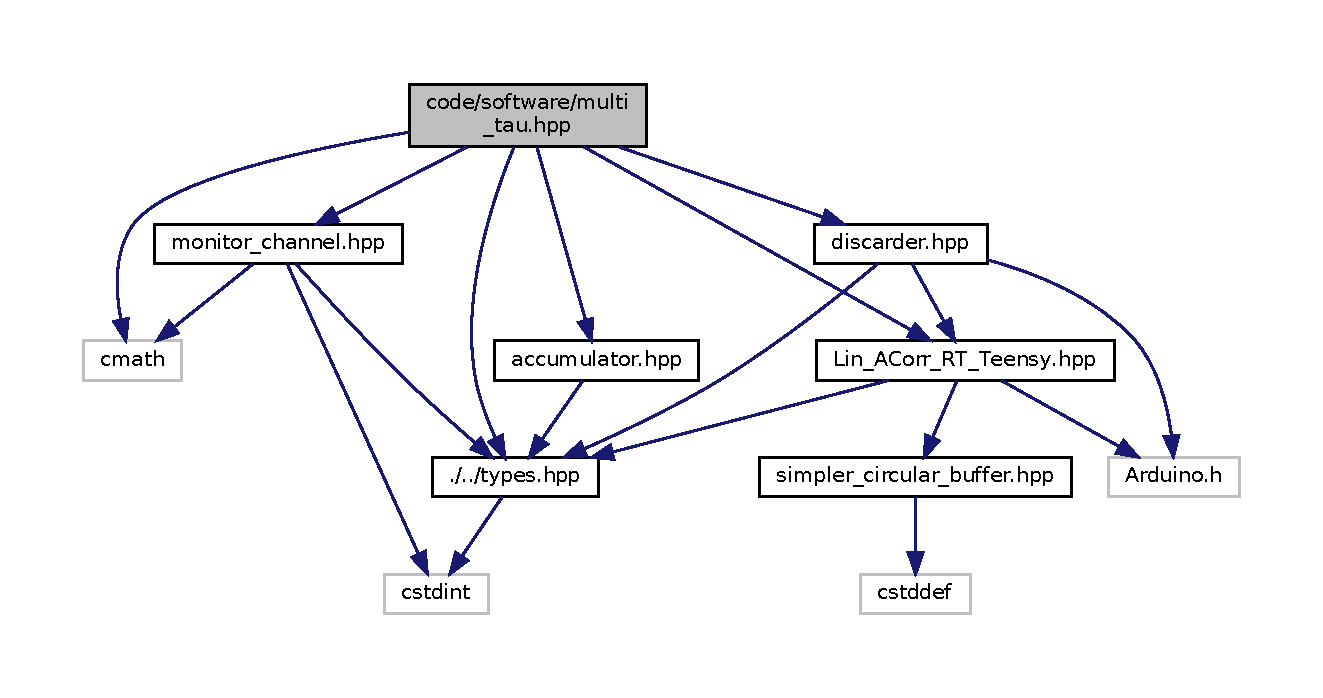
\includegraphics[width=350pt]{de/df4/multi__tau_8hpp__incl}
\end{center}
\end{figure}
This graph shows which files directly or indirectly include this file\+:
\nopagebreak
\begin{figure}[H]
\begin{center}
\leavevmode
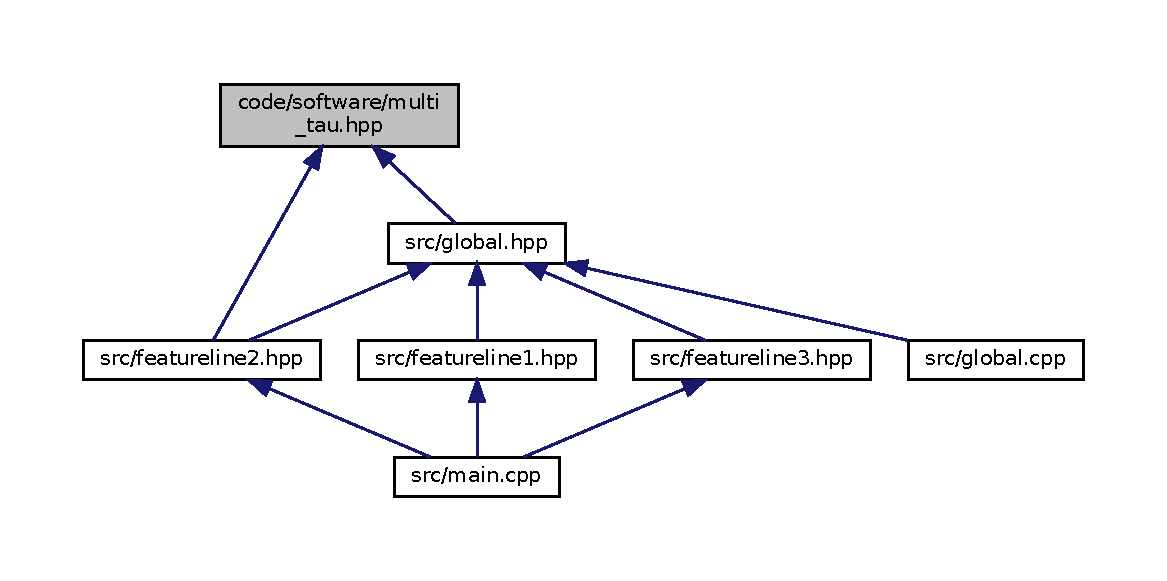
\includegraphics[width=350pt]{d3/d49/multi__tau_8hpp__dep__incl}
\end{center}
\end{figure}
\subsection*{Classes}
\begin{DoxyCompactItemize}
\item 
class \hyperlink{classMultiTauACorrRTTeensy}{Multi\+Tau\+A\+Corr\+R\+T\+Teensy$<$ Lin\+\_\+channels, Series\+\_\+size, Bin\+\_\+\+Ratio $>$}
\begin{DoxyCompactList}\small\item\em Multi\+Tau Auto-\/\+Correlator object that is composed of multiple linear -\/ autocorrelators. Specialised for teensy. \end{DoxyCompactList}\end{DoxyCompactItemize}

\hypertarget{pseudoSerial_8cpp}{}\section{code/software/pseudo\+Serial.cpp File Reference}
\label{pseudoSerial_8cpp}\index{code/software/pseudo\+Serial.\+cpp@{code/software/pseudo\+Serial.\+cpp}}

\hypertarget{pseudoSerial_8hpp}{}\section{code/software/pseudo\+Serial.hpp File Reference}
\label{pseudoSerial_8hpp}\index{code/software/pseudo\+Serial.\+hpp@{code/software/pseudo\+Serial.\+hpp}}

\hypertarget{simpler__circular__buffer_8hpp}{}\section{lib/software/simpler\+\_\+circular\+\_\+buffer.hpp File Reference}
\label{simpler__circular__buffer_8hpp}\index{lib/software/simpler\+\_\+circular\+\_\+buffer.\+hpp@{lib/software/simpler\+\_\+circular\+\_\+buffer.\+hpp}}
{\ttfamily \#include $<$cstddef$>$}\newline
Include dependency graph for simpler\+\_\+circular\+\_\+buffer.\+hpp\+:
\nopagebreak
\begin{figure}[H]
\begin{center}
\leavevmode
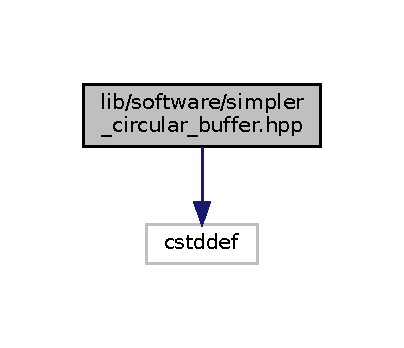
\includegraphics[width=194pt]{simpler__circular__buffer_8hpp__incl}
\end{center}
\end{figure}
\subsection*{Classes}
\begin{DoxyCompactItemize}
\item 
class \hyperlink{classSimpler__Circular__Buffer}{Simpler\+\_\+\+Circular\+\_\+\+Buffer$<$ Type, Max\+Size $>$}
\end{DoxyCompactItemize}

\hypertarget{test_8cpp}{}\section{code/software/test.cpp File Reference}
\label{test_8cpp}\index{code/software/test.\+cpp@{code/software/test.\+cpp}}

\hypertarget{types_8hpp}{}\section{code/types.hpp File Reference}
\label{types_8hpp}\index{code/types.\+hpp@{code/types.\+hpp}}
{\ttfamily \#include $<$cstdint$>$}\newline
Include dependency graph for types.\+hpp\+:\nopagebreak
\begin{figure}[H]
\begin{center}
\leavevmode
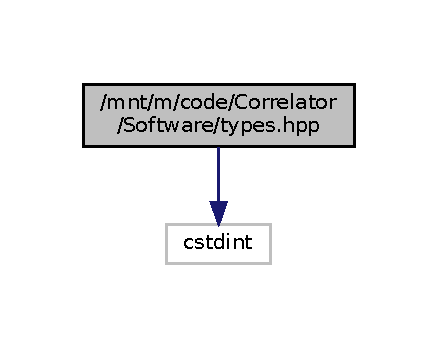
\includegraphics[width=171pt]{types_8hpp__incl}
\end{center}
\end{figure}
This graph shows which files directly or indirectly include this file\+:
\nopagebreak
\begin{figure}[H]
\begin{center}
\leavevmode
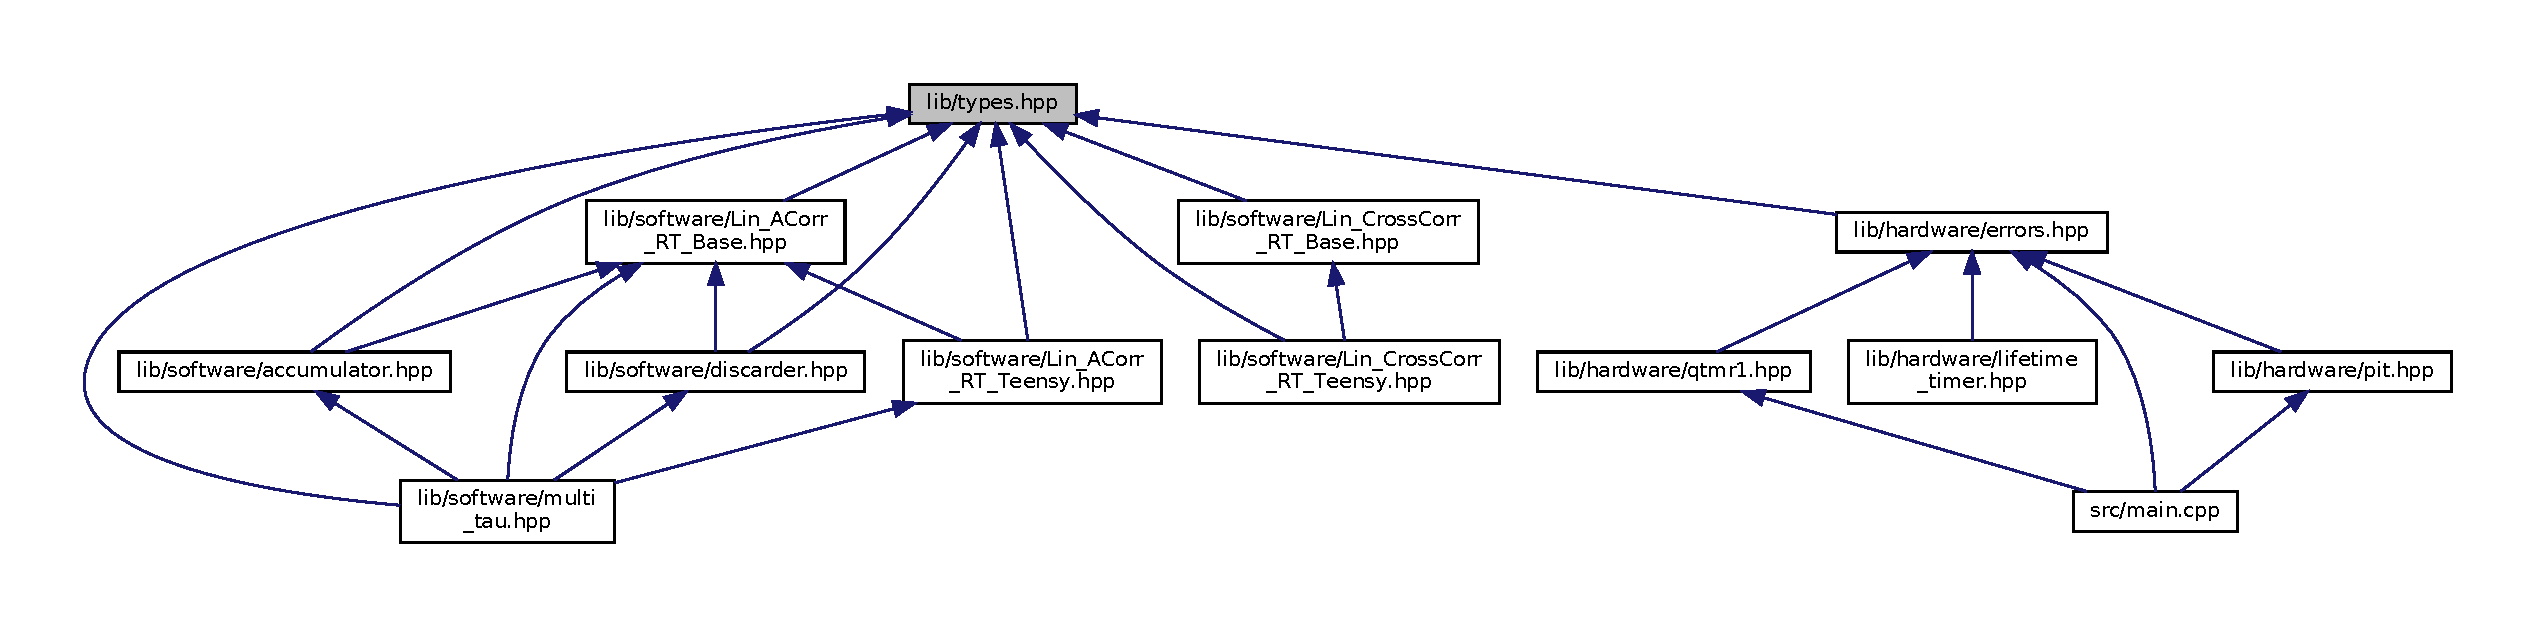
\includegraphics[width=350pt]{types_8hpp__dep__incl}
\end{center}
\end{figure}
\subsection*{Typedefs}
\begin{DoxyCompactItemize}
\item 
using \hyperlink{types_8hpp_a22f279793847eba127de149437848c48}{counter\+\_\+t} = uint32\+\_\+t
\begin{DoxyCompactList}\small\item\em Data type received from the pulse counter. It is the fundamental type used for representing series data. \end{DoxyCompactList}\item 
using \hyperlink{types_8hpp_a7c40bb931c31595ed6308605f4537447}{index\+\_\+t} = uint\+\_\+fast8\+\_\+t
\begin{DoxyCompactList}\small\item\em It is used as the array indices and thus determine the maximum size of the Channel\+\_\+array and the Series\+\_\+array. \end{DoxyCompactList}\end{DoxyCompactItemize}


\subsection{Typedef Documentation}
\mbox{\Hypertarget{types_8hpp_a22f279793847eba127de149437848c48}\label{types_8hpp_a22f279793847eba127de149437848c48}} 
\index{types.\+hpp@{types.\+hpp}!counter\+\_\+t@{counter\+\_\+t}}
\index{counter\+\_\+t@{counter\+\_\+t}!types.\+hpp@{types.\+hpp}}
\subsubsection{\texorpdfstring{counter\+\_\+t}{counter\_t}}
{\footnotesize\ttfamily using \hyperlink{types_8hpp_a22f279793847eba127de149437848c48}{counter\+\_\+t} =  uint32\+\_\+t}



Data type received from the pulse counter. It is the fundamental type used for representing series data. 

\mbox{\Hypertarget{types_8hpp_a7c40bb931c31595ed6308605f4537447}\label{types_8hpp_a7c40bb931c31595ed6308605f4537447}} 
\index{types.\+hpp@{types.\+hpp}!index\+\_\+t@{index\+\_\+t}}
\index{index\+\_\+t@{index\+\_\+t}!types.\+hpp@{types.\+hpp}}
\subsubsection{\texorpdfstring{index\+\_\+t}{index\_t}}
{\footnotesize\ttfamily using \hyperlink{types_8hpp_a7c40bb931c31595ed6308605f4537447}{index\+\_\+t} =  uint\+\_\+fast8\+\_\+t}



It is used as the array indices and thus determine the maximum size of the Channel\+\_\+array and the Series\+\_\+array. 


\hypertarget{README_8md}{}\section{R\+E\+A\+D\+M\+E.\+md File Reference}
\label{README_8md}\index{R\+E\+A\+D\+M\+E.\+md@{R\+E\+A\+D\+M\+E.\+md}}

\hypertarget{code_2software_2README_8md}{}\section{code/software/\+R\+E\+A\+D\+ME.md File Reference}
\label{code_2software_2README_8md}\index{code/software/\+R\+E\+A\+D\+M\+E.\+md@{code/software/\+R\+E\+A\+D\+M\+E.\+md}}

\hypertarget{code_2hardware_2README_8md}{}\section{code/hardware/\+R\+E\+A\+D\+ME.md File Reference}
\label{code_2hardware_2README_8md}\index{code/hardware/\+R\+E\+A\+D\+M\+E.\+md@{code/hardware/\+R\+E\+A\+D\+M\+E.\+md}}

\hypertarget{featureline1_8hpp}{}\section{src/featureline1.hpp File Reference}
\label{featureline1_8hpp}\index{src/featureline1.\+hpp@{src/featureline1.\+hpp}}
{\ttfamily \#include $<$Arduino.\+h$>$}\newline
{\ttfamily \#include $<$imxrt.\+h$>$}\newline
{\ttfamily \#include \char`\"{}global.\+hpp\char`\"{}}\newline
{\ttfamily \#include \char`\"{}./../code/software/monitor\+\_\+channel.\+hpp\char`\"{}}\newline
{\ttfamily \#include \char`\"{}./../code/software/histogram.\+hpp\char`\"{}}\newline
{\ttfamily \#include \char`\"{}./../code/hardware/pins.\+hpp\char`\"{}}\newline
{\ttfamily \#include \char`\"{}./../code/hardware/utilities.\+hpp\char`\"{}}\newline
{\ttfamily \#include \char`\"{}./../code/hardware/ledpanel.\+hpp\char`\"{}}\newline
{\ttfamily \#include \char`\"{}./../code/hardware/errors.\+hpp\char`\"{}}\newline
{\ttfamily \#include \char`\"{}./../code/hardware/pit.\+hpp\char`\"{}}\newline
{\ttfamily \#include \char`\"{}./../code/hardware/qtmr1.\+hpp\char`\"{}}\newline
{\ttfamily \#include \char`\"{}./../code/hardware/perf\+\_\+counter.\+hpp\char`\"{}}\newline
Include dependency graph for featureline1.\+hpp\+:
\nopagebreak
\begin{figure}[H]
\begin{center}
\leavevmode
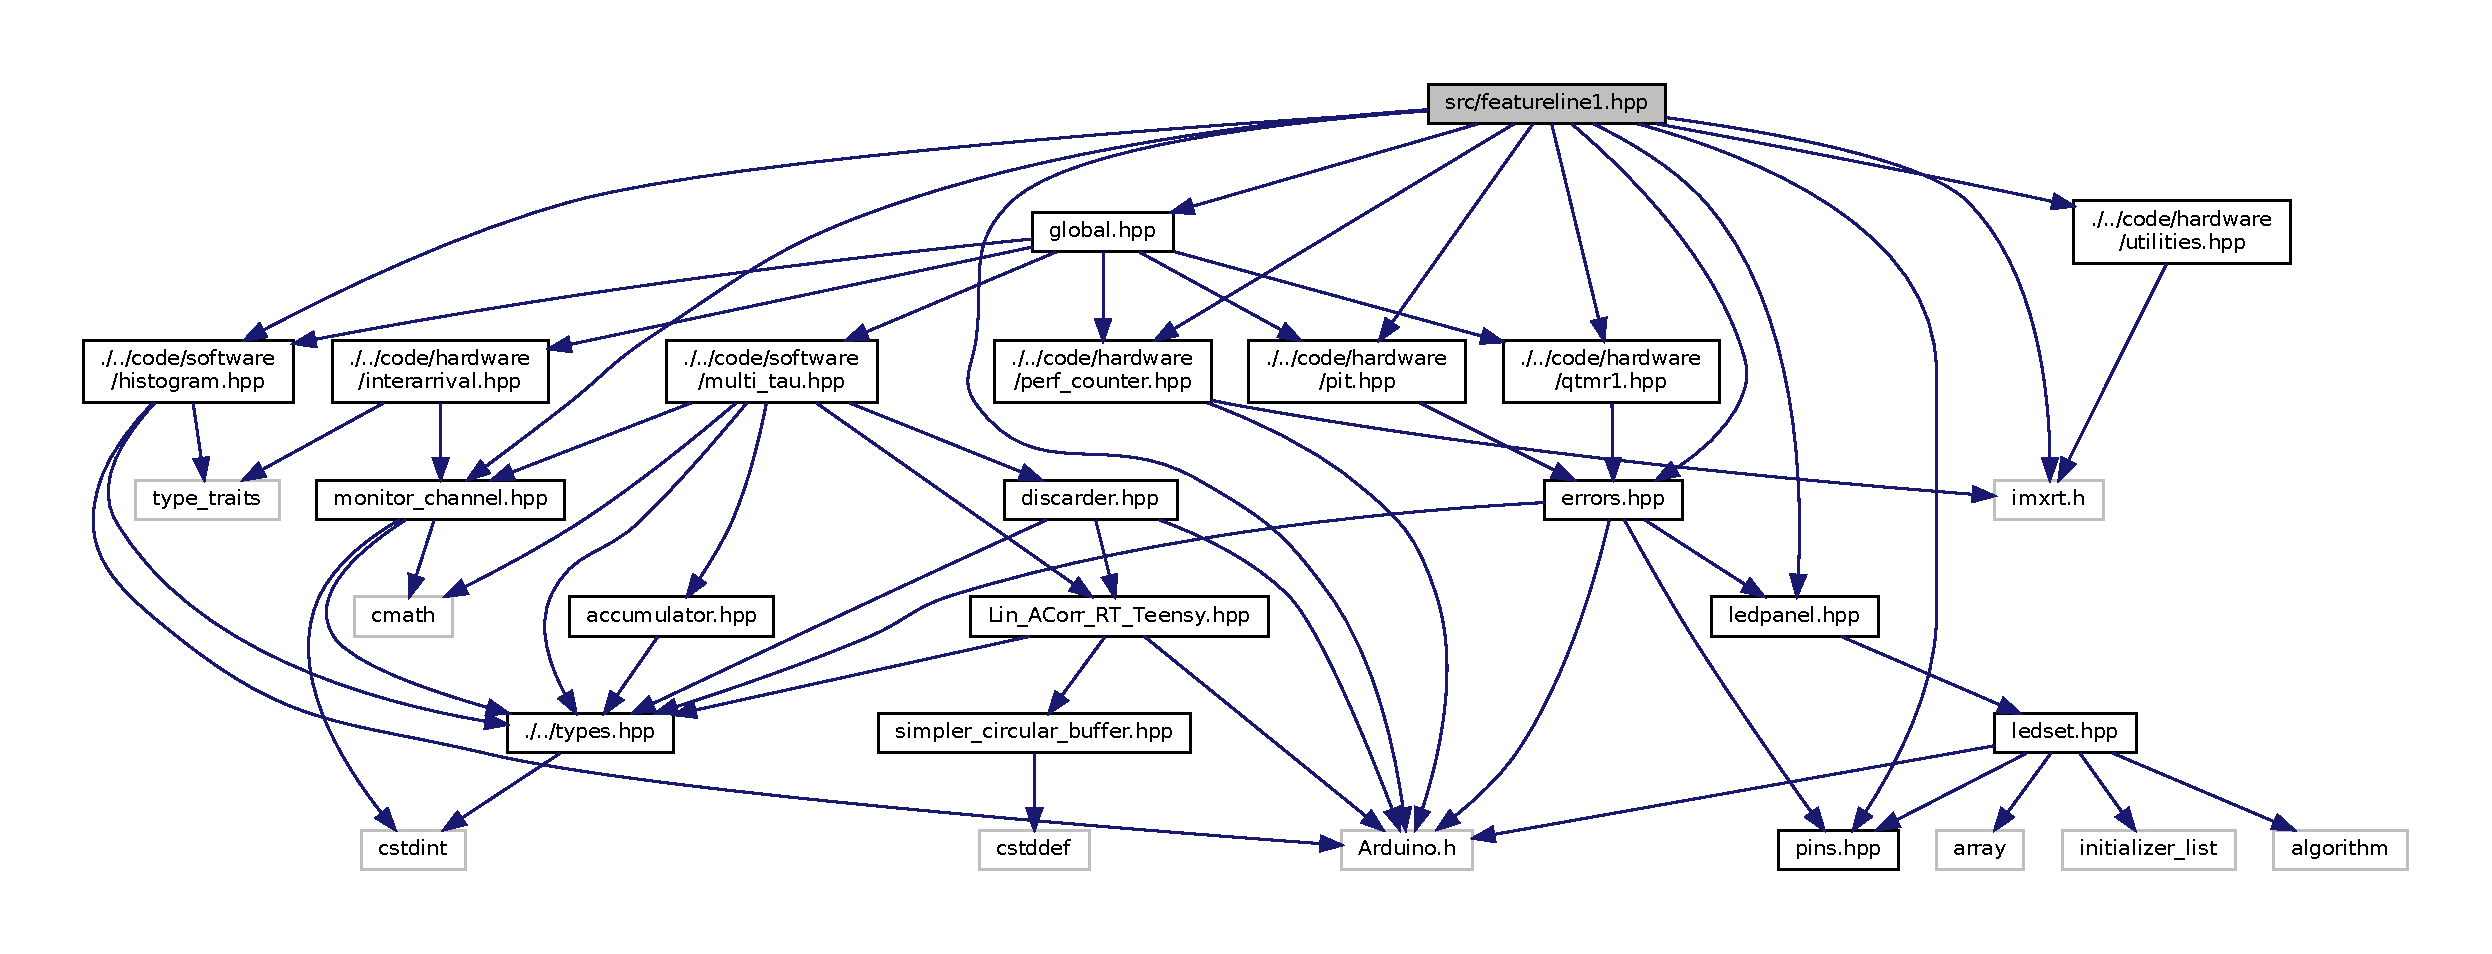
\includegraphics[width=350pt]{d2/df8/featureline1_8hpp__incl}
\end{center}
\end{figure}
This graph shows which files directly or indirectly include this file\+:
\nopagebreak
\begin{figure}[H]
\begin{center}
\leavevmode
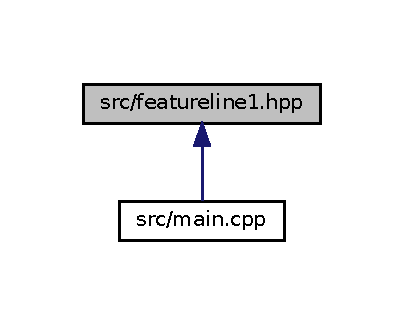
\includegraphics[width=194pt]{d5/de8/featureline1_8hpp__dep__incl}
\end{center}
\end{figure}
\subsection*{Functions}
\begin{DoxyCompactItemize}
\item 
void \hyperlink{featureline1_8hpp_a4fc8f622f69a856a51bd3d4b1b42233a}{isr\+\_\+fn} ()
\begin{DoxyCompactList}\small\item\em I\+SR function used for processing counter values. \end{DoxyCompactList}\item 
void \hyperlink{featureline1_8hpp_af81803d7af0f109d27e4bcc2859eb398}{serial\+\_\+out} ()
\begin{DoxyCompactList}\small\item\em Outputs the data struct to the serial buffer. \end{DoxyCompactList}\item 
void \hyperlink{featureline1_8hpp_a1d39ca49552cf7468c736db6854309ff}{gt\+\_\+setup} ()
\begin{DoxyCompactList}\small\item\em Setup function for Initalization and setup. \end{DoxyCompactList}\item 
void \hyperlink{featureline1_8hpp_aa9c34f2e013f03846aee63202bf56c43}{gt\+\_\+loop} ()
\begin{DoxyCompactList}\small\item\em Loop function that processes the updates from the counters. \end{DoxyCompactList}\end{DoxyCompactItemize}


\subsection{Function Documentation}
\mbox{\Hypertarget{featureline1_8hpp_aa9c34f2e013f03846aee63202bf56c43}\label{featureline1_8hpp_aa9c34f2e013f03846aee63202bf56c43}} 
\index{featureline1.\+hpp@{featureline1.\+hpp}!gt\+\_\+loop@{gt\+\_\+loop}}
\index{gt\+\_\+loop@{gt\+\_\+loop}!featureline1.\+hpp@{featureline1.\+hpp}}
\subsubsection{\texorpdfstring{gt\+\_\+loop()}{gt\_loop()}}
{\footnotesize\ttfamily void gt\+\_\+loop (\begin{DoxyParamCaption}{ }\end{DoxyParamCaption})}



Loop function that processes the updates from the counters. 

\mbox{\Hypertarget{featureline1_8hpp_a1d39ca49552cf7468c736db6854309ff}\label{featureline1_8hpp_a1d39ca49552cf7468c736db6854309ff}} 
\index{featureline1.\+hpp@{featureline1.\+hpp}!gt\+\_\+setup@{gt\+\_\+setup}}
\index{gt\+\_\+setup@{gt\+\_\+setup}!featureline1.\+hpp@{featureline1.\+hpp}}
\subsubsection{\texorpdfstring{gt\+\_\+setup()}{gt\_setup()}}
{\footnotesize\ttfamily void gt\+\_\+setup (\begin{DoxyParamCaption}{ }\end{DoxyParamCaption})}



Setup function for Initalization and setup. 

\mbox{\Hypertarget{featureline1_8hpp_a4fc8f622f69a856a51bd3d4b1b42233a}\label{featureline1_8hpp_a4fc8f622f69a856a51bd3d4b1b42233a}} 
\index{featureline1.\+hpp@{featureline1.\+hpp}!isr\+\_\+fn@{isr\+\_\+fn}}
\index{isr\+\_\+fn@{isr\+\_\+fn}!featureline1.\+hpp@{featureline1.\+hpp}}
\subsubsection{\texorpdfstring{isr\+\_\+fn()}{isr\_fn()}}
{\footnotesize\ttfamily void isr\+\_\+fn (\begin{DoxyParamCaption}{ }\end{DoxyParamCaption})}



I\+SR function used for processing counter values. 

\mbox{\Hypertarget{featureline1_8hpp_af81803d7af0f109d27e4bcc2859eb398}\label{featureline1_8hpp_af81803d7af0f109d27e4bcc2859eb398}} 
\index{featureline1.\+hpp@{featureline1.\+hpp}!serial\+\_\+out@{serial\+\_\+out}}
\index{serial\+\_\+out@{serial\+\_\+out}!featureline1.\+hpp@{featureline1.\+hpp}}
\subsubsection{\texorpdfstring{serial\+\_\+out()}{serial\_out()}}
{\footnotesize\ttfamily void serial\+\_\+out (\begin{DoxyParamCaption}{ }\end{DoxyParamCaption})\hspace{0.3cm}{\ttfamily [inline]}}



Outputs the data struct to the serial buffer. 


\hypertarget{featureline2_8hpp}{}\section{src/featureline2.hpp File Reference}
\label{featureline2_8hpp}\index{src/featureline2.\+hpp@{src/featureline2.\+hpp}}
{\ttfamily \#include $<$Arduino.\+h$>$}\newline
{\ttfamily \#include $<$imxrt.\+h$>$}\newline
{\ttfamily \#include \char`\"{}global.\+hpp\char`\"{}}\newline
{\ttfamily \#include \char`\"{}./../code/hardware/qtmr1.\+hpp\char`\"{}}\newline
{\ttfamily \#include \char`\"{}./../code/hardware/ledpanel.\+hpp\char`\"{}}\newline
{\ttfamily \#include \char`\"{}./../code/software/multi\+\_\+tau.\+hpp\char`\"{}}\newline
Include dependency graph for featureline2.\+hpp\+:
\nopagebreak
\begin{figure}[H]
\begin{center}
\leavevmode
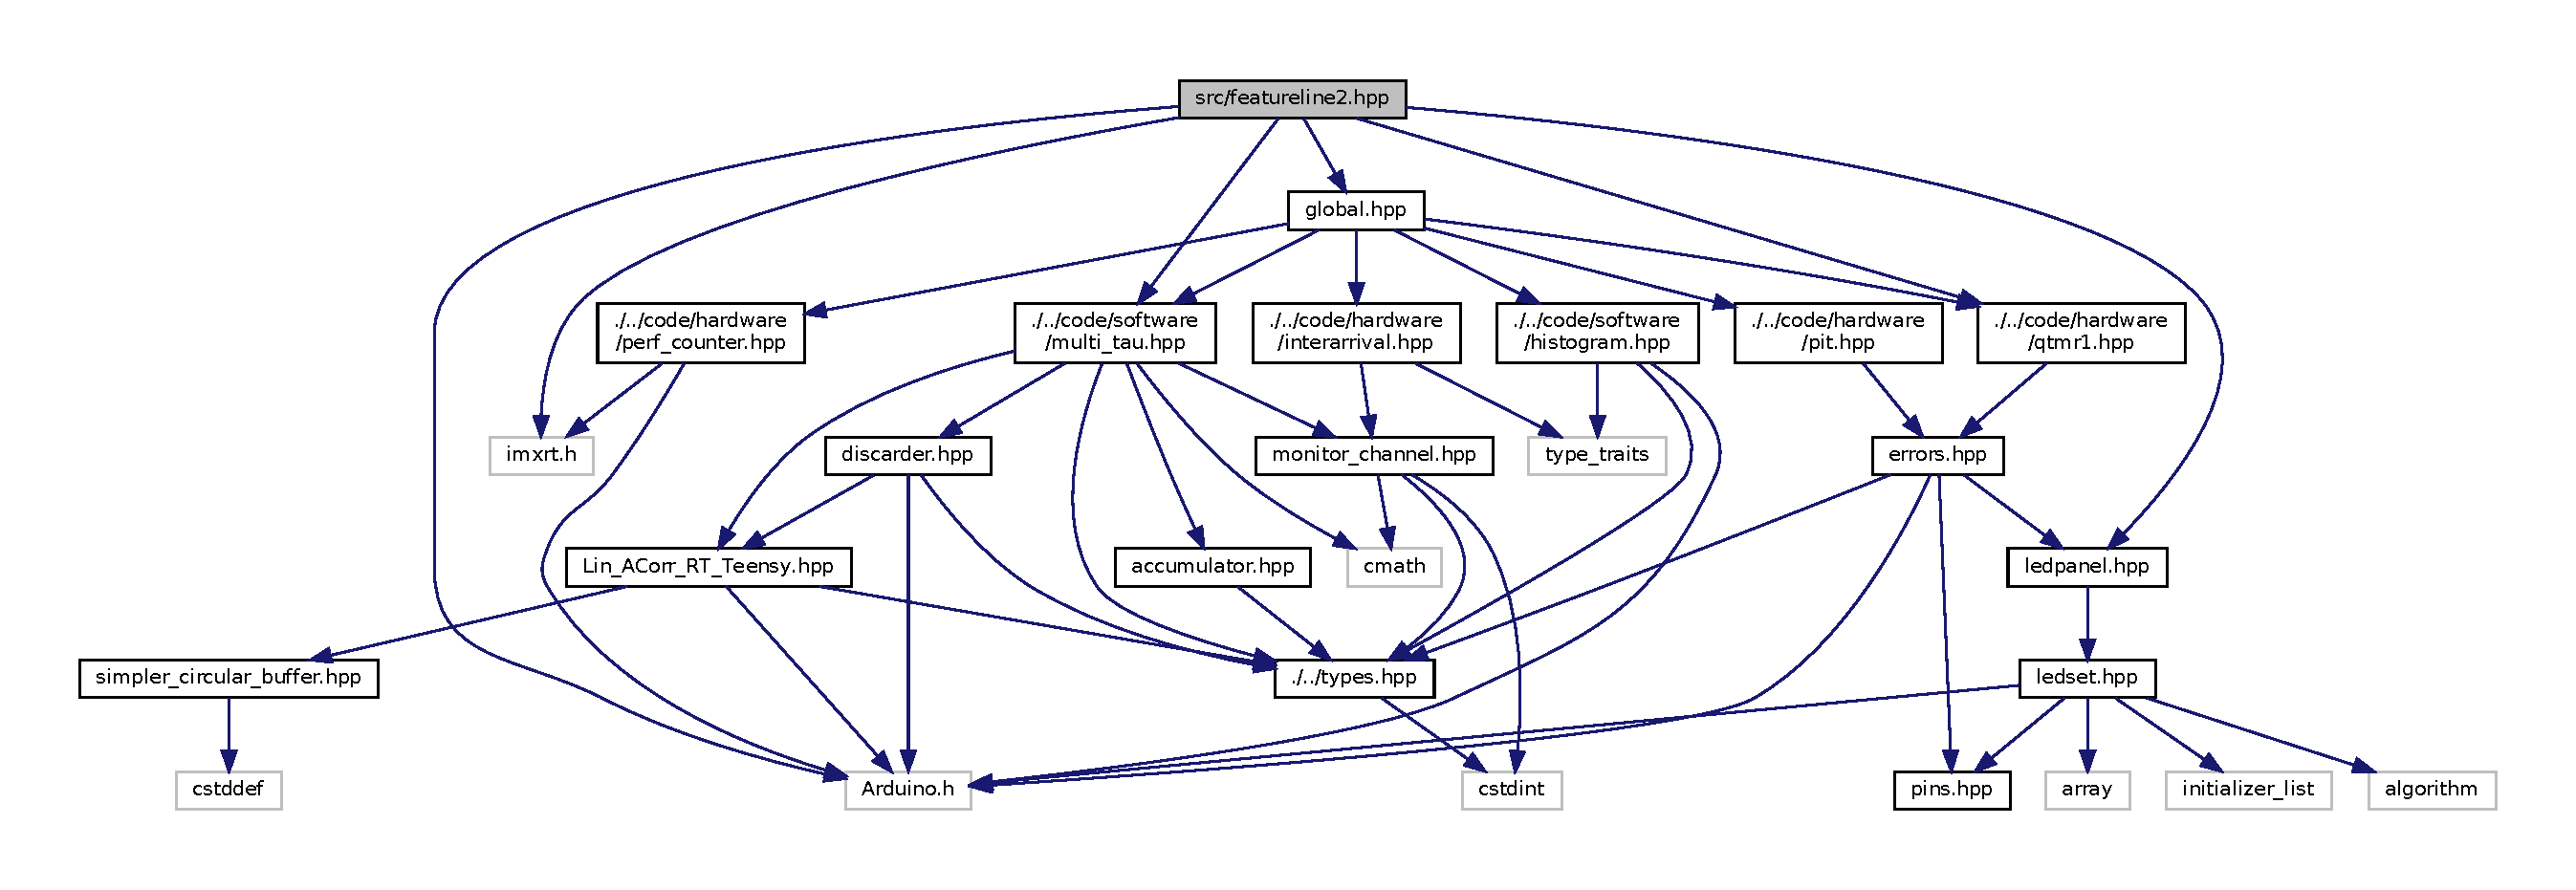
\includegraphics[width=350pt]{featureline2_8hpp__incl}
\end{center}
\end{figure}
This graph shows which files directly or indirectly include this file\+:
\nopagebreak
\begin{figure}[H]
\begin{center}
\leavevmode
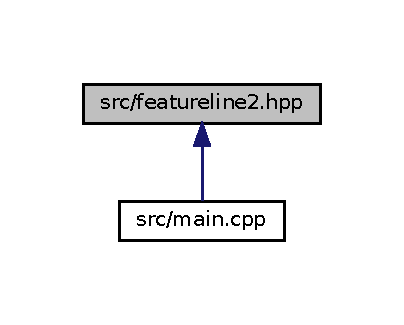
\includegraphics[width=194pt]{featureline2_8hpp__dep__incl}
\end{center}
\end{figure}
\subsection*{Functions}
\begin{DoxyCompactItemize}
\item 
void \hyperlink{featureline2_8hpp_a2f630755ed6ea8b32810b12b33b9871f}{setup\+\_\+interarrival} ()
\item 
void \hyperlink{featureline2_8hpp_a0f61e7bed45e41724d4370e1a8b09952}{loop\+\_\+interarrival} ()
\end{DoxyCompactItemize}


\subsection{Function Documentation}
\mbox{\Hypertarget{featureline2_8hpp_a0f61e7bed45e41724d4370e1a8b09952}\label{featureline2_8hpp_a0f61e7bed45e41724d4370e1a8b09952}} 
\index{featureline2.\+hpp@{featureline2.\+hpp}!loop\+\_\+interarrival@{loop\+\_\+interarrival}}
\index{loop\+\_\+interarrival@{loop\+\_\+interarrival}!featureline2.\+hpp@{featureline2.\+hpp}}
\subsubsection{\texorpdfstring{loop\+\_\+interarrival()}{loop\_interarrival()}}
{\footnotesize\ttfamily void loop\+\_\+interarrival (\begin{DoxyParamCaption}{ }\end{DoxyParamCaption})}

\mbox{\Hypertarget{featureline2_8hpp_a2f630755ed6ea8b32810b12b33b9871f}\label{featureline2_8hpp_a2f630755ed6ea8b32810b12b33b9871f}} 
\index{featureline2.\+hpp@{featureline2.\+hpp}!setup\+\_\+interarrival@{setup\+\_\+interarrival}}
\index{setup\+\_\+interarrival@{setup\+\_\+interarrival}!featureline2.\+hpp@{featureline2.\+hpp}}
\subsubsection{\texorpdfstring{setup\+\_\+interarrival()}{setup\_interarrival()}}
{\footnotesize\ttfamily void setup\+\_\+interarrival (\begin{DoxyParamCaption}{ }\end{DoxyParamCaption})}


\hypertarget{featureline3_8hpp}{}\section{src/featureline3.hpp File Reference}
\label{featureline3_8hpp}\index{src/featureline3.\+hpp@{src/featureline3.\+hpp}}
{\ttfamily \#include $<$Arduino.\+h$>$}\newline
{\ttfamily \#include $<$imxrt.\+h$>$}\newline
{\ttfamily \#include \char`\"{}global.\+hpp\char`\"{}}\newline
{\ttfamily \#include \char`\"{}./../code/hardware/pins.\+hpp\char`\"{}}\newline
{\ttfamily \#include \char`\"{}./../code/hardware/ledpanel.\+hpp\char`\"{}}\newline
{\ttfamily \#include \char`\"{}./../code/hardware/errors.\+hpp\char`\"{}}\newline
{\ttfamily \#include \char`\"{}./../code/hardware/pit.\+hpp\char`\"{}}\newline
{\ttfamily \#include \char`\"{}./../code/hardware/qtmr1.\+hpp\char`\"{}}\newline
{\ttfamily \#include \char`\"{}./../code/software/monitor\+\_\+channel.\+hpp\char`\"{}}\newline
Include dependency graph for featureline3.\+hpp\+:
\nopagebreak
\begin{figure}[H]
\begin{center}
\leavevmode
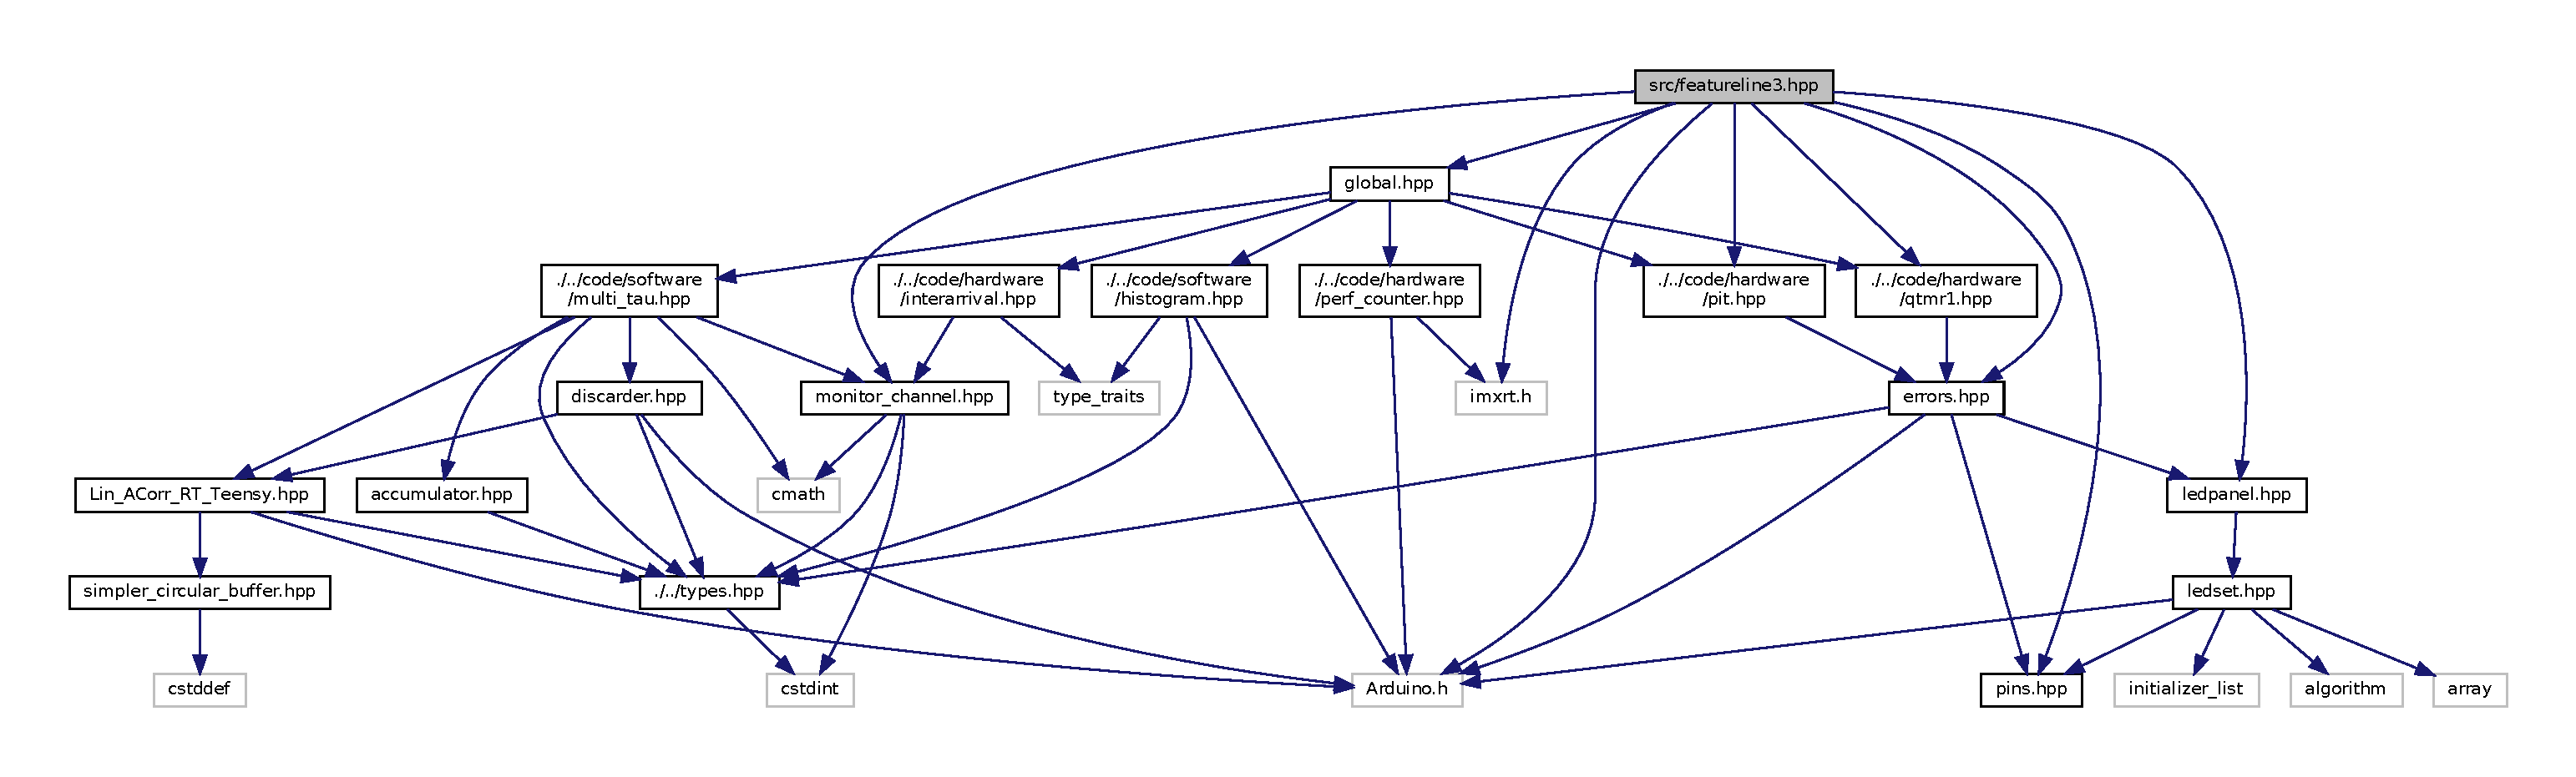
\includegraphics[width=350pt]{d8/d17/featureline3_8hpp__incl}
\end{center}
\end{figure}
This graph shows which files directly or indirectly include this file\+:
\nopagebreak
\begin{figure}[H]
\begin{center}
\leavevmode
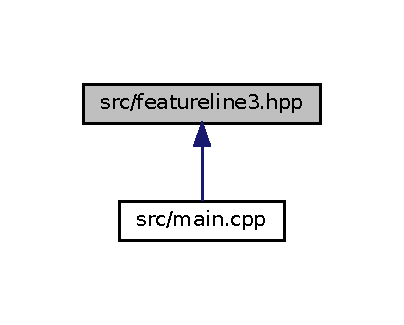
\includegraphics[width=194pt]{d3/d0b/featureline3_8hpp__dep__incl}
\end{center}
\end{figure}
\subsection*{Functions}
\begin{DoxyCompactItemize}
\item 
void \hyperlink{featureline3_8hpp_a25ace3177d8ee7b01dc98fd605f07ee8}{isr\+\_\+fn3} ()
\begin{DoxyCompactList}\small\item\em This featureline (see {\ttfamily featurelines.\+md) samples Counter values at periodic intervals and prints it to the Serial buffer(using}println(){\ttfamily ). This machinary is a subset of}$\ast$featureline1$\ast$`, which is the complete Gate Counting featureline. \end{DoxyCompactList}\item 
void \hyperlink{featureline3_8hpp_a13ba355c388354ef55c85e39c02b6b20}{sampler\+\_\+setup} ()
\item 
void \hyperlink{featureline3_8hpp_acaf2bd0b8ea25302fbcfd07139c11a86}{sampler\+\_\+loop} ()
\end{DoxyCompactItemize}


\subsection{Function Documentation}
\mbox{\Hypertarget{featureline3_8hpp_a25ace3177d8ee7b01dc98fd605f07ee8}\label{featureline3_8hpp_a25ace3177d8ee7b01dc98fd605f07ee8}} 
\index{featureline3.\+hpp@{featureline3.\+hpp}!isr\+\_\+fn3@{isr\+\_\+fn3}}
\index{isr\+\_\+fn3@{isr\+\_\+fn3}!featureline3.\+hpp@{featureline3.\+hpp}}
\subsubsection{\texorpdfstring{isr\+\_\+fn3()}{isr\_fn3()}}
{\footnotesize\ttfamily void isr\+\_\+fn3 (\begin{DoxyParamCaption}{ }\end{DoxyParamCaption})}



This featureline (see {\ttfamily featurelines.\+md) samples Counter values at periodic intervals and prints it to the Serial buffer(using}println(){\ttfamily ). This machinary is a subset of}$\ast$featureline1$\ast$`, which is the complete Gate Counting featureline. 

\mbox{\Hypertarget{featureline3_8hpp_acaf2bd0b8ea25302fbcfd07139c11a86}\label{featureline3_8hpp_acaf2bd0b8ea25302fbcfd07139c11a86}} 
\index{featureline3.\+hpp@{featureline3.\+hpp}!sampler\+\_\+loop@{sampler\+\_\+loop}}
\index{sampler\+\_\+loop@{sampler\+\_\+loop}!featureline3.\+hpp@{featureline3.\+hpp}}
\subsubsection{\texorpdfstring{sampler\+\_\+loop()}{sampler\_loop()}}
{\footnotesize\ttfamily void sampler\+\_\+loop (\begin{DoxyParamCaption}{ }\end{DoxyParamCaption})}

\mbox{\Hypertarget{featureline3_8hpp_a13ba355c388354ef55c85e39c02b6b20}\label{featureline3_8hpp_a13ba355c388354ef55c85e39c02b6b20}} 
\index{featureline3.\+hpp@{featureline3.\+hpp}!sampler\+\_\+setup@{sampler\+\_\+setup}}
\index{sampler\+\_\+setup@{sampler\+\_\+setup}!featureline3.\+hpp@{featureline3.\+hpp}}
\subsubsection{\texorpdfstring{sampler\+\_\+setup()}{sampler\_setup()}}
{\footnotesize\ttfamily void sampler\+\_\+setup (\begin{DoxyParamCaption}{ }\end{DoxyParamCaption})}


\hypertarget{global_8cpp}{}\section{src/global.cpp File Reference}
\label{global_8cpp}\index{src/global.\+cpp@{src/global.\+cpp}}
{\ttfamily \#include \char`\"{}global.\+hpp\char`\"{}}\newline
Include dependency graph for global.\+cpp\+:
\nopagebreak
\begin{figure}[H]
\begin{center}
\leavevmode
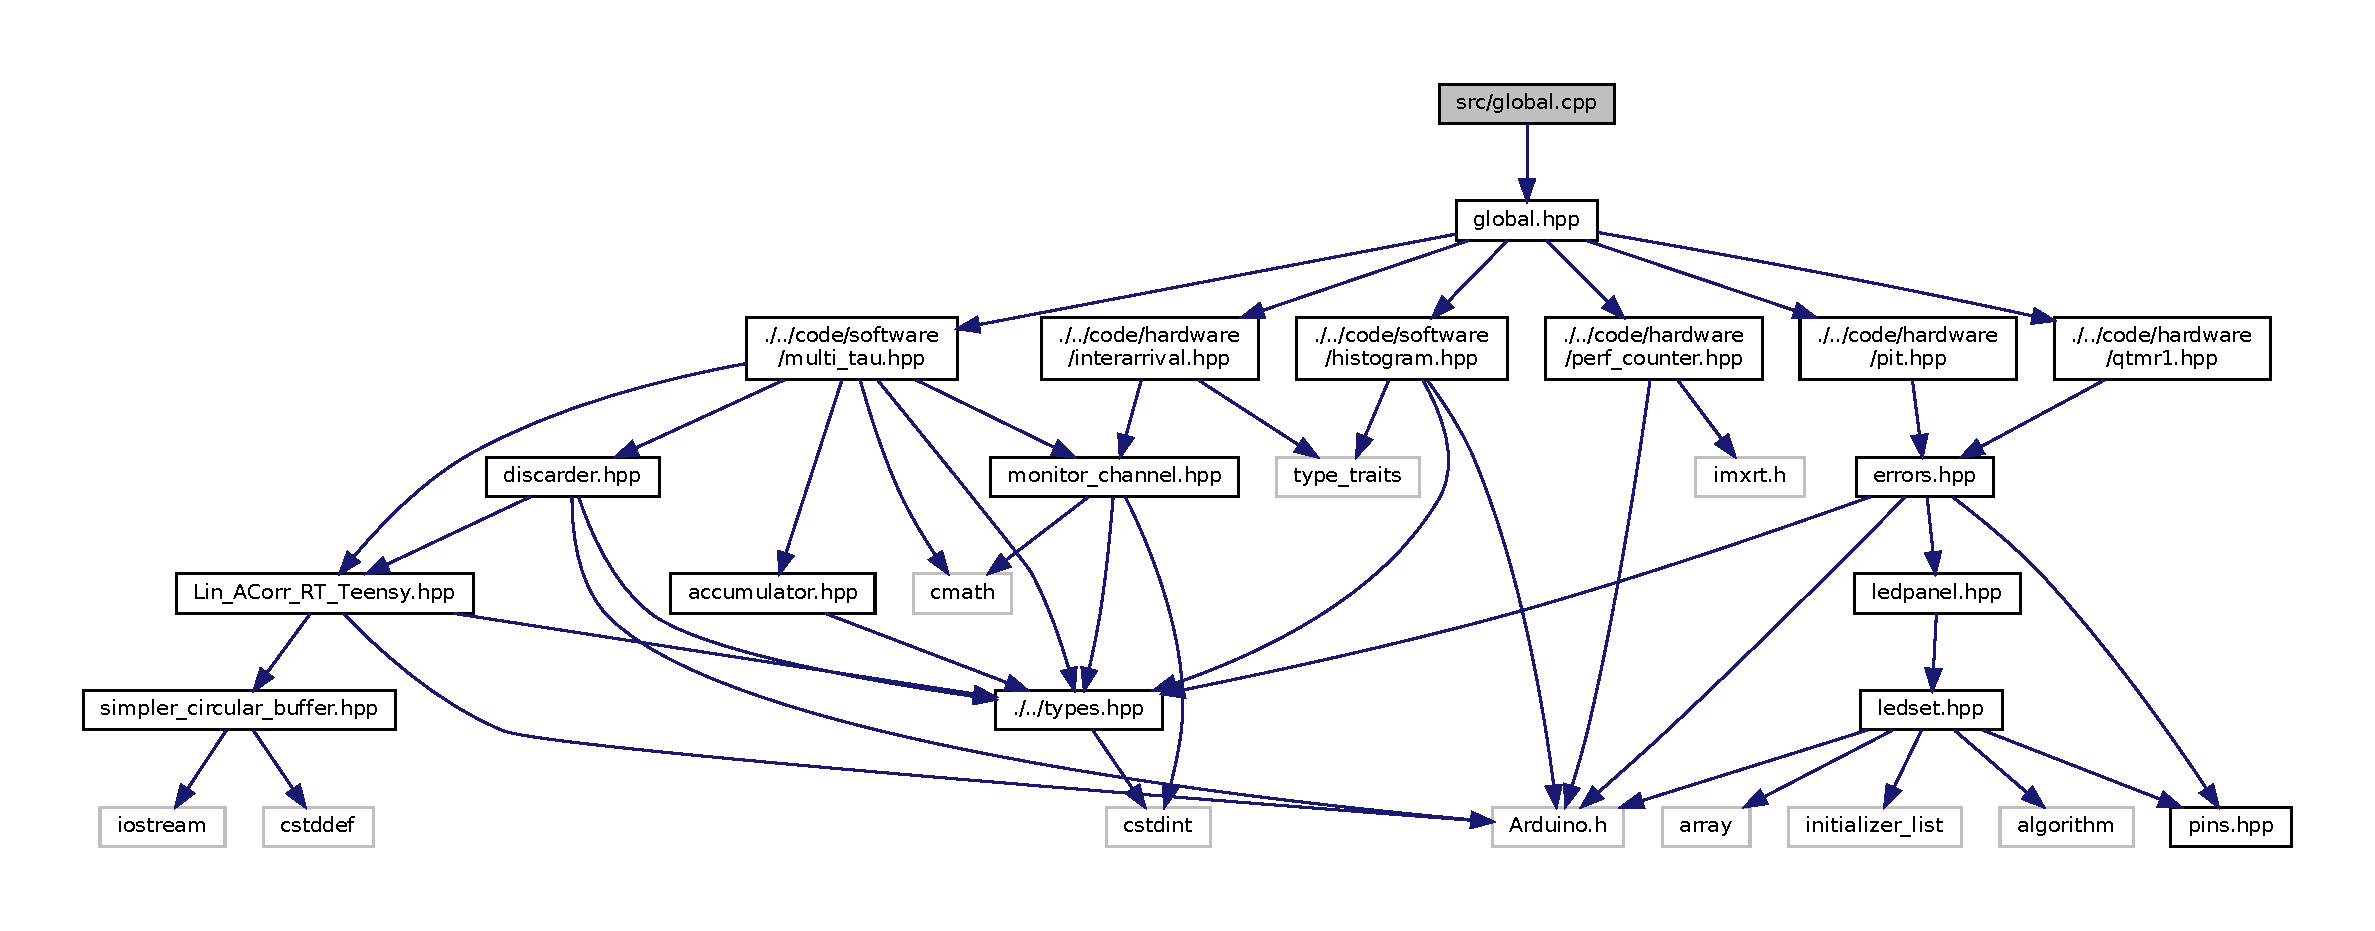
\includegraphics[width=350pt]{global_8cpp__incl}
\end{center}
\end{figure}
\subsection*{Variables}
\begin{DoxyCompactItemize}
\item 
\hyperlink{classMultiTauACorrRTTeensy}{Multi\+Tau\+A\+Corr\+R\+T\+Teensy}$<$ L\+I\+N\+\_\+\+C\+O\+R\+RS, S\+E\+R\+I\+E\+S\+\_\+\+S\+I\+ZE, B\+I\+N\+\_\+\+R\+A\+T\+IO $>$ \hyperlink{global_8cpp_ac9447f67aa187aba18d60e3fd3a51bd3}{multitau}
\item 
\hyperlink{classPITController}{P\+I\+T\+Controller}$<$ P\+I\+T\+\_\+\+C\+H\+A\+N\+N\+E\+L\+\_\+\+I\+N\+\_\+\+U\+SE $>$ \hyperlink{global_8cpp_af11c331fc1c91504e3f7d2dccf67b739}{P\+I\+\_\+t}
\begin{DoxyCompactList}\small\item\em P\+I\+\_\+t Resource. \end{DoxyCompactList}\item 
\hyperlink{classTMR1Controller}{T\+M\+R1\+Controller} \hyperlink{global_8cpp_a691981c43e1bdddca6df5accb6927331}{T\+T\+L\+\_\+c}
\begin{DoxyCompactList}\small\item\em T\+T\+L\+\_\+c Resource. \end{DoxyCompactList}\item 
volatile \hyperlink{types_8hpp_a22f279793847eba127de149437848c48}{counter\+\_\+t} \hyperlink{global_8cpp_afcac7adcea259024440f8d9257d82d08}{Counter\+\_\+val} = 0
\begin{DoxyCompactList}\small\item\em Stores the value read from the counter. \end{DoxyCompactList}\item 
volatile bool \hyperlink{global_8cpp_afaf7617e9ce0486d54a6c65fedeaf1f9}{Update\+\_\+flag} = false
\begin{DoxyCompactList}\small\item\em Indicates if a new value has arrived from the counting module. \end{DoxyCompactList}\item 
volatile unsigned int \hyperlink{global_8cpp_aec1fbfd9bfc90e447b39a9362a0c51de}{Update\+\_\+count} = 0
\begin{DoxyCompactList}\small\item\em Stores the number of updates made on the correlator channels since the last serialout. \end{DoxyCompactList}\item 
uint32\+\_\+t \hyperlink{global_8cpp_a7687ee385c82b3ac600720b79678755a}{Serial\+Out\+\_\+\+After} = 100
\item 
const double \hyperlink{global_8cpp_a1d18182f432f5b88cf58be9c367be457}{Gate\+\_\+time\+\_\+us} = G\+A\+T\+E\+\_\+\+T\+I\+M\+E\+\_\+\+US
\begin{DoxyCompactList}\small\item\em Serial output is done after these many updates (default → overriden in the setup function). \end{DoxyCompactList}\item 
const double \hyperlink{global_8cpp_ada17f1639ca8a5932f17942031baa67f}{Allowed\+\_\+period\+\_\+error\+\_\+us} = A\+L\+L\+O\+W\+E\+D\+\_\+\+G\+A\+T\+E\+\_\+\+T\+I\+M\+E\+\_\+\+E\+R\+R\+O\+R\+\_\+\+US
\begin{DoxyCompactList}\small\item\em The gate time of T\+T\+L\+\_\+C in microseconds (us) \end{DoxyCompactList}\item 
const int32\+\_\+t \hyperlink{global_8cpp_abaef541ea152f1c10c21aab606888f1b}{sync\+\_\+code} = S\+Y\+N\+C\+\_\+\+C\+O\+DE
\begin{DoxyCompactList}\small\item\em Gate time precision error due to finite precision of timers. \end{DoxyCompactList}\item 
float \hyperlink{global_8cpp_ac6c0b94aa91631e1cf6f4f55e97c52b2}{array} \mbox{[}C\+H\+A\+N\+N\+E\+L\+\_\+\+S\+I\+ZE\mbox{]} = \{0\}
\end{DoxyCompactItemize}


\subsection{Variable Documentation}
\mbox{\Hypertarget{global_8cpp_ada17f1639ca8a5932f17942031baa67f}\label{global_8cpp_ada17f1639ca8a5932f17942031baa67f}} 
\index{global.\+cpp@{global.\+cpp}!Allowed\+\_\+period\+\_\+error\+\_\+us@{Allowed\+\_\+period\+\_\+error\+\_\+us}}
\index{Allowed\+\_\+period\+\_\+error\+\_\+us@{Allowed\+\_\+period\+\_\+error\+\_\+us}!global.\+cpp@{global.\+cpp}}
\subsubsection{\texorpdfstring{Allowed\+\_\+period\+\_\+error\+\_\+us}{Allowed\_period\_error\_us}}
{\footnotesize\ttfamily const double Allowed\+\_\+period\+\_\+error\+\_\+us = A\+L\+L\+O\+W\+E\+D\+\_\+\+G\+A\+T\+E\+\_\+\+T\+I\+M\+E\+\_\+\+E\+R\+R\+O\+R\+\_\+\+US}



The gate time of T\+T\+L\+\_\+C in microseconds (us) 

\mbox{\Hypertarget{global_8cpp_ac6c0b94aa91631e1cf6f4f55e97c52b2}\label{global_8cpp_ac6c0b94aa91631e1cf6f4f55e97c52b2}} 
\index{global.\+cpp@{global.\+cpp}!array@{array}}
\index{array@{array}!global.\+cpp@{global.\+cpp}}
\subsubsection{\texorpdfstring{array}{array}}
{\footnotesize\ttfamily float array\mbox{[}C\+H\+A\+N\+N\+E\+L\+\_\+\+S\+I\+ZE\mbox{]} = \{0\}}

\mbox{\Hypertarget{global_8cpp_afcac7adcea259024440f8d9257d82d08}\label{global_8cpp_afcac7adcea259024440f8d9257d82d08}} 
\index{global.\+cpp@{global.\+cpp}!Counter\+\_\+val@{Counter\+\_\+val}}
\index{Counter\+\_\+val@{Counter\+\_\+val}!global.\+cpp@{global.\+cpp}}
\subsubsection{\texorpdfstring{Counter\+\_\+val}{Counter\_val}}
{\footnotesize\ttfamily volatile \hyperlink{types_8hpp_a22f279793847eba127de149437848c48}{counter\+\_\+t} Counter\+\_\+val = 0}



Stores the value read from the counter. 

\mbox{\Hypertarget{global_8cpp_a1d18182f432f5b88cf58be9c367be457}\label{global_8cpp_a1d18182f432f5b88cf58be9c367be457}} 
\index{global.\+cpp@{global.\+cpp}!Gate\+\_\+time\+\_\+us@{Gate\+\_\+time\+\_\+us}}
\index{Gate\+\_\+time\+\_\+us@{Gate\+\_\+time\+\_\+us}!global.\+cpp@{global.\+cpp}}
\subsubsection{\texorpdfstring{Gate\+\_\+time\+\_\+us}{Gate\_time\_us}}
{\footnotesize\ttfamily const double Gate\+\_\+time\+\_\+us = G\+A\+T\+E\+\_\+\+T\+I\+M\+E\+\_\+\+US}



Serial output is done after these many updates (default → overriden in the setup function). 

\mbox{\Hypertarget{global_8cpp_ac9447f67aa187aba18d60e3fd3a51bd3}\label{global_8cpp_ac9447f67aa187aba18d60e3fd3a51bd3}} 
\index{global.\+cpp@{global.\+cpp}!multitau@{multitau}}
\index{multitau@{multitau}!global.\+cpp@{global.\+cpp}}
\subsubsection{\texorpdfstring{multitau}{multitau}}
{\footnotesize\ttfamily \hyperlink{classMultiTauACorrRTTeensy}{Multi\+Tau\+A\+Corr\+R\+T\+Teensy}$<$L\+I\+N\+\_\+\+C\+O\+R\+RS, S\+E\+R\+I\+E\+S\+\_\+\+S\+I\+ZE, B\+I\+N\+\_\+\+R\+A\+T\+IO$>$ multitau}

\mbox{\Hypertarget{global_8cpp_af11c331fc1c91504e3f7d2dccf67b739}\label{global_8cpp_af11c331fc1c91504e3f7d2dccf67b739}} 
\index{global.\+cpp@{global.\+cpp}!P\+I\+\_\+t@{P\+I\+\_\+t}}
\index{P\+I\+\_\+t@{P\+I\+\_\+t}!global.\+cpp@{global.\+cpp}}
\subsubsection{\texorpdfstring{P\+I\+\_\+t}{PI\_t}}
{\footnotesize\ttfamily \hyperlink{classPITController}{P\+I\+T\+Controller}$<$P\+I\+T\+\_\+\+C\+H\+A\+N\+N\+E\+L\+\_\+\+I\+N\+\_\+\+U\+SE$>$ P\+I\+\_\+t}



P\+I\+\_\+t Resource. 

\mbox{\Hypertarget{global_8cpp_a7687ee385c82b3ac600720b79678755a}\label{global_8cpp_a7687ee385c82b3ac600720b79678755a}} 
\index{global.\+cpp@{global.\+cpp}!Serial\+Out\+\_\+\+After@{Serial\+Out\+\_\+\+After}}
\index{Serial\+Out\+\_\+\+After@{Serial\+Out\+\_\+\+After}!global.\+cpp@{global.\+cpp}}
\subsubsection{\texorpdfstring{Serial\+Out\+\_\+\+After}{SerialOut\_After}}
{\footnotesize\ttfamily uint32\+\_\+t Serial\+Out\+\_\+\+After = 100}

\mbox{\Hypertarget{global_8cpp_abaef541ea152f1c10c21aab606888f1b}\label{global_8cpp_abaef541ea152f1c10c21aab606888f1b}} 
\index{global.\+cpp@{global.\+cpp}!sync\+\_\+code@{sync\+\_\+code}}
\index{sync\+\_\+code@{sync\+\_\+code}!global.\+cpp@{global.\+cpp}}
\subsubsection{\texorpdfstring{sync\+\_\+code}{sync\_code}}
{\footnotesize\ttfamily const int32\+\_\+t sync\+\_\+code = S\+Y\+N\+C\+\_\+\+C\+O\+DE}



Gate time precision error due to finite precision of timers. 

\mbox{\Hypertarget{global_8cpp_a691981c43e1bdddca6df5accb6927331}\label{global_8cpp_a691981c43e1bdddca6df5accb6927331}} 
\index{global.\+cpp@{global.\+cpp}!T\+T\+L\+\_\+c@{T\+T\+L\+\_\+c}}
\index{T\+T\+L\+\_\+c@{T\+T\+L\+\_\+c}!global.\+cpp@{global.\+cpp}}
\subsubsection{\texorpdfstring{T\+T\+L\+\_\+c}{TTL\_c}}
{\footnotesize\ttfamily \hyperlink{classTMR1Controller}{T\+M\+R1\+Controller} T\+T\+L\+\_\+c}



T\+T\+L\+\_\+c Resource. 

\mbox{\Hypertarget{global_8cpp_aec1fbfd9bfc90e447b39a9362a0c51de}\label{global_8cpp_aec1fbfd9bfc90e447b39a9362a0c51de}} 
\index{global.\+cpp@{global.\+cpp}!Update\+\_\+count@{Update\+\_\+count}}
\index{Update\+\_\+count@{Update\+\_\+count}!global.\+cpp@{global.\+cpp}}
\subsubsection{\texorpdfstring{Update\+\_\+count}{Update\_count}}
{\footnotesize\ttfamily volatile unsigned int Update\+\_\+count = 0}



Stores the number of updates made on the correlator channels since the last serialout. 

\mbox{\Hypertarget{global_8cpp_afaf7617e9ce0486d54a6c65fedeaf1f9}\label{global_8cpp_afaf7617e9ce0486d54a6c65fedeaf1f9}} 
\index{global.\+cpp@{global.\+cpp}!Update\+\_\+flag@{Update\+\_\+flag}}
\index{Update\+\_\+flag@{Update\+\_\+flag}!global.\+cpp@{global.\+cpp}}
\subsubsection{\texorpdfstring{Update\+\_\+flag}{Update\_flag}}
{\footnotesize\ttfamily volatile bool Update\+\_\+flag = false}



Indicates if a new value has arrived from the counting module. 


\hypertarget{global_8hpp}{}\section{src/global.hpp File Reference}
\label{global_8hpp}\index{src/global.\+hpp@{src/global.\+hpp}}
{\ttfamily \#include \char`\"{}./../code/software/multi\+\_\+tau.\+hpp\char`\"{}}\newline
{\ttfamily \#include \char`\"{}./../code/software/histogram.\+hpp\char`\"{}}\newline
{\ttfamily \#include \char`\"{}./../code/hardware/pit.\+hpp\char`\"{}}\newline
{\ttfamily \#include \char`\"{}./../code/hardware/qtmr1.\+hpp\char`\"{}}\newline
{\ttfamily \#include \char`\"{}./../code/hardware/interarrival.\+hpp\char`\"{}}\newline
{\ttfamily \#include \char`\"{}./../code/hardware/perf\+\_\+counter.\+hpp\char`\"{}}\newline
Include dependency graph for global.\+hpp\+:
\nopagebreak
\begin{figure}[H]
\begin{center}
\leavevmode
\includegraphics[width=350pt]{global_8hpp__incl}
\end{center}
\end{figure}
This graph shows which files directly or indirectly include this file\+:
\nopagebreak
\begin{figure}[H]
\begin{center}
\leavevmode
\includegraphics[width=350pt]{global_8hpp__dep__incl}
\end{center}
\end{figure}
\subsection*{Variables}
\begin{DoxyCompactItemize}
\item 
\hyperlink{classMultiTauACorrRTTeensy}{Multi\+Tau\+A\+Corr\+R\+T\+Teensy}$<$ L\+I\+N\+\_\+\+C\+O\+R\+RS, S\+E\+R\+I\+E\+S\+\_\+\+S\+I\+ZE, B\+I\+N\+\_\+\+R\+A\+T\+IO $>$ \hyperlink{global_8hpp_ac9447f67aa187aba18d60e3fd3a51bd3}{multitau}
\item 
\hyperlink{classPITController}{P\+I\+T\+Controller}$<$ P\+I\+T\+\_\+\+C\+H\+A\+N\+N\+E\+L\+\_\+\+I\+N\+\_\+\+U\+SE $>$ \hyperlink{global_8hpp_af11c331fc1c91504e3f7d2dccf67b739}{P\+I\+\_\+t}
\begin{DoxyCompactList}\small\item\em P\+I\+\_\+t Resource. \end{DoxyCompactList}\item 
\hyperlink{classTMR1Controller}{T\+M\+R1\+Controller} \hyperlink{global_8hpp_a691981c43e1bdddca6df5accb6927331}{T\+T\+L\+\_\+c}
\begin{DoxyCompactList}\small\item\em T\+T\+L\+\_\+c Resource. \end{DoxyCompactList}\item 
volatile \hyperlink{types_8hpp_a22f279793847eba127de149437848c48}{counter\+\_\+t} \hyperlink{global_8hpp_afcac7adcea259024440f8d9257d82d08}{Counter\+\_\+val}
\begin{DoxyCompactList}\small\item\em Stores the value read from the counter. \end{DoxyCompactList}\item 
volatile bool \hyperlink{global_8hpp_afaf7617e9ce0486d54a6c65fedeaf1f9}{Update\+\_\+flag}
\begin{DoxyCompactList}\small\item\em Indicates if a new value has arrived from the counting module. \end{DoxyCompactList}\item 
volatile unsigned int \hyperlink{global_8hpp_aec1fbfd9bfc90e447b39a9362a0c51de}{Update\+\_\+count}
\begin{DoxyCompactList}\small\item\em Stores the number of updates made on the correlator channels since the last serialout. \end{DoxyCompactList}\item 
uint32\+\_\+t \hyperlink{global_8hpp_a7687ee385c82b3ac600720b79678755a}{Serial\+Out\+\_\+\+After}
\item 
const double \hyperlink{global_8hpp_a1d18182f432f5b88cf58be9c367be457}{Gate\+\_\+time\+\_\+us}
\begin{DoxyCompactList}\small\item\em Serial output is done after these many updates (default → overriden in the setup function). \end{DoxyCompactList}\item 
const double \hyperlink{global_8hpp_ada17f1639ca8a5932f17942031baa67f}{Allowed\+\_\+period\+\_\+error\+\_\+us}
\begin{DoxyCompactList}\small\item\em The gate time of T\+T\+L\+\_\+C in microseconds (us) \end{DoxyCompactList}\item 
const int32\+\_\+t \hyperlink{global_8hpp_abaef541ea152f1c10c21aab606888f1b}{sync\+\_\+code}
\begin{DoxyCompactList}\small\item\em Gate time precision error due to finite precision of timers. \end{DoxyCompactList}\item 
float \hyperlink{global_8hpp_ac6c0b94aa91631e1cf6f4f55e97c52b2}{array} \mbox{[}C\+H\+A\+N\+N\+E\+L\+\_\+\+S\+I\+ZE\mbox{]}
\end{DoxyCompactItemize}


\subsection{Variable Documentation}
\mbox{\Hypertarget{global_8hpp_ada17f1639ca8a5932f17942031baa67f}\label{global_8hpp_ada17f1639ca8a5932f17942031baa67f}} 
\index{global.\+hpp@{global.\+hpp}!Allowed\+\_\+period\+\_\+error\+\_\+us@{Allowed\+\_\+period\+\_\+error\+\_\+us}}
\index{Allowed\+\_\+period\+\_\+error\+\_\+us@{Allowed\+\_\+period\+\_\+error\+\_\+us}!global.\+hpp@{global.\+hpp}}
\subsubsection{\texorpdfstring{Allowed\+\_\+period\+\_\+error\+\_\+us}{Allowed\_period\_error\_us}}
{\footnotesize\ttfamily const double Allowed\+\_\+period\+\_\+error\+\_\+us}



The gate time of T\+T\+L\+\_\+C in microseconds (us) 

\mbox{\Hypertarget{global_8hpp_ac6c0b94aa91631e1cf6f4f55e97c52b2}\label{global_8hpp_ac6c0b94aa91631e1cf6f4f55e97c52b2}} 
\index{global.\+hpp@{global.\+hpp}!array@{array}}
\index{array@{array}!global.\+hpp@{global.\+hpp}}
\subsubsection{\texorpdfstring{array}{array}}
{\footnotesize\ttfamily float array\mbox{[}C\+H\+A\+N\+N\+E\+L\+\_\+\+S\+I\+ZE\mbox{]}}

\mbox{\Hypertarget{global_8hpp_afcac7adcea259024440f8d9257d82d08}\label{global_8hpp_afcac7adcea259024440f8d9257d82d08}} 
\index{global.\+hpp@{global.\+hpp}!Counter\+\_\+val@{Counter\+\_\+val}}
\index{Counter\+\_\+val@{Counter\+\_\+val}!global.\+hpp@{global.\+hpp}}
\subsubsection{\texorpdfstring{Counter\+\_\+val}{Counter\_val}}
{\footnotesize\ttfamily volatile \hyperlink{types_8hpp_a22f279793847eba127de149437848c48}{counter\+\_\+t} Counter\+\_\+val}



Stores the value read from the counter. 

\mbox{\Hypertarget{global_8hpp_a1d18182f432f5b88cf58be9c367be457}\label{global_8hpp_a1d18182f432f5b88cf58be9c367be457}} 
\index{global.\+hpp@{global.\+hpp}!Gate\+\_\+time\+\_\+us@{Gate\+\_\+time\+\_\+us}}
\index{Gate\+\_\+time\+\_\+us@{Gate\+\_\+time\+\_\+us}!global.\+hpp@{global.\+hpp}}
\subsubsection{\texorpdfstring{Gate\+\_\+time\+\_\+us}{Gate\_time\_us}}
{\footnotesize\ttfamily const double Gate\+\_\+time\+\_\+us}



Serial output is done after these many updates (default → overriden in the setup function). 

\mbox{\Hypertarget{global_8hpp_ac9447f67aa187aba18d60e3fd3a51bd3}\label{global_8hpp_ac9447f67aa187aba18d60e3fd3a51bd3}} 
\index{global.\+hpp@{global.\+hpp}!multitau@{multitau}}
\index{multitau@{multitau}!global.\+hpp@{global.\+hpp}}
\subsubsection{\texorpdfstring{multitau}{multitau}}
{\footnotesize\ttfamily \hyperlink{classMultiTauACorrRTTeensy}{Multi\+Tau\+A\+Corr\+R\+T\+Teensy}$<$L\+I\+N\+\_\+\+C\+O\+R\+RS, S\+E\+R\+I\+E\+S\+\_\+\+S\+I\+ZE, B\+I\+N\+\_\+\+R\+A\+T\+IO$>$ multitau}

\mbox{\Hypertarget{global_8hpp_af11c331fc1c91504e3f7d2dccf67b739}\label{global_8hpp_af11c331fc1c91504e3f7d2dccf67b739}} 
\index{global.\+hpp@{global.\+hpp}!P\+I\+\_\+t@{P\+I\+\_\+t}}
\index{P\+I\+\_\+t@{P\+I\+\_\+t}!global.\+hpp@{global.\+hpp}}
\subsubsection{\texorpdfstring{P\+I\+\_\+t}{PI\_t}}
{\footnotesize\ttfamily \hyperlink{classPITController}{P\+I\+T\+Controller}$<$P\+I\+T\+\_\+\+C\+H\+A\+N\+N\+E\+L\+\_\+\+I\+N\+\_\+\+U\+SE$>$ P\+I\+\_\+t}



P\+I\+\_\+t Resource. 

\mbox{\Hypertarget{global_8hpp_a7687ee385c82b3ac600720b79678755a}\label{global_8hpp_a7687ee385c82b3ac600720b79678755a}} 
\index{global.\+hpp@{global.\+hpp}!Serial\+Out\+\_\+\+After@{Serial\+Out\+\_\+\+After}}
\index{Serial\+Out\+\_\+\+After@{Serial\+Out\+\_\+\+After}!global.\+hpp@{global.\+hpp}}
\subsubsection{\texorpdfstring{Serial\+Out\+\_\+\+After}{SerialOut\_After}}
{\footnotesize\ttfamily uint32\+\_\+t Serial\+Out\+\_\+\+After}

\mbox{\Hypertarget{global_8hpp_abaef541ea152f1c10c21aab606888f1b}\label{global_8hpp_abaef541ea152f1c10c21aab606888f1b}} 
\index{global.\+hpp@{global.\+hpp}!sync\+\_\+code@{sync\+\_\+code}}
\index{sync\+\_\+code@{sync\+\_\+code}!global.\+hpp@{global.\+hpp}}
\subsubsection{\texorpdfstring{sync\+\_\+code}{sync\_code}}
{\footnotesize\ttfamily const int32\+\_\+t sync\+\_\+code}



Gate time precision error due to finite precision of timers. 

\mbox{\Hypertarget{global_8hpp_a691981c43e1bdddca6df5accb6927331}\label{global_8hpp_a691981c43e1bdddca6df5accb6927331}} 
\index{global.\+hpp@{global.\+hpp}!T\+T\+L\+\_\+c@{T\+T\+L\+\_\+c}}
\index{T\+T\+L\+\_\+c@{T\+T\+L\+\_\+c}!global.\+hpp@{global.\+hpp}}
\subsubsection{\texorpdfstring{T\+T\+L\+\_\+c}{TTL\_c}}
{\footnotesize\ttfamily \hyperlink{classTMR1Controller}{T\+M\+R1\+Controller} T\+T\+L\+\_\+c}



T\+T\+L\+\_\+c Resource. 

\mbox{\Hypertarget{global_8hpp_aec1fbfd9bfc90e447b39a9362a0c51de}\label{global_8hpp_aec1fbfd9bfc90e447b39a9362a0c51de}} 
\index{global.\+hpp@{global.\+hpp}!Update\+\_\+count@{Update\+\_\+count}}
\index{Update\+\_\+count@{Update\+\_\+count}!global.\+hpp@{global.\+hpp}}
\subsubsection{\texorpdfstring{Update\+\_\+count}{Update\_count}}
{\footnotesize\ttfamily volatile unsigned int Update\+\_\+count}



Stores the number of updates made on the correlator channels since the last serialout. 

\mbox{\Hypertarget{global_8hpp_afaf7617e9ce0486d54a6c65fedeaf1f9}\label{global_8hpp_afaf7617e9ce0486d54a6c65fedeaf1f9}} 
\index{global.\+hpp@{global.\+hpp}!Update\+\_\+flag@{Update\+\_\+flag}}
\index{Update\+\_\+flag@{Update\+\_\+flag}!global.\+hpp@{global.\+hpp}}
\subsubsection{\texorpdfstring{Update\+\_\+flag}{Update\_flag}}
{\footnotesize\ttfamily volatile bool Update\+\_\+flag}



Indicates if a new value has arrived from the counting module. 


\hypertarget{ledpanel_8cpp}{}\section{src/ledpanel.cpp File Reference}
\label{ledpanel_8cpp}\index{src/ledpanel.\+cpp@{src/ledpanel.\+cpp}}
{\ttfamily \#include \char`\"{}./../code/hardware/ledpanel.\+hpp\char`\"{}}\newline
Include dependency graph for ledpanel.\+cpp\+:
\nopagebreak
\begin{figure}[H]
\begin{center}
\leavevmode
\includegraphics[width=350pt]{ledpanel_8cpp__incl}
\end{center}
\end{figure}
\subsection*{Variables}
\begin{DoxyCompactItemize}
\item 
\hyperlink{classLEDSet}{L\+E\+D\+Set}$<$ 5 $>$ \hyperlink{ledpanel_8cpp_a4400ea46c721995dc7815cfe422c028d}{L\+E\+D\+Panel} (\{L\+E\+D\+\_\+\+B\+U\+I\+L\+T\+IN, \hyperlink{pins_8hpp_a735f426a390e22c0050b964328c5e06f}{L\+E\+D\+\_\+\+R\+ED}, \hyperlink{pins_8hpp_a8d7df4222b2fde6205bebffc5a0ae070}{L\+E\+D\+\_\+\+G\+R\+E\+EN}, \hyperlink{pins_8hpp_a1be903f86639d50fb6ed02a0dbbe0e2c}{L\+E\+D\+\_\+\+W\+H\+I\+TE}, \hyperlink{pins_8hpp_a8046eca6ddcbe578777cfde489622a13}{L\+E\+D\+\_\+\+B\+L\+UE}\})
\end{DoxyCompactItemize}


\subsection{Variable Documentation}
\mbox{\Hypertarget{ledpanel_8cpp_a4400ea46c721995dc7815cfe422c028d}\label{ledpanel_8cpp_a4400ea46c721995dc7815cfe422c028d}} 
\index{ledpanel.\+cpp@{ledpanel.\+cpp}!L\+E\+D\+Panel@{L\+E\+D\+Panel}}
\index{L\+E\+D\+Panel@{L\+E\+D\+Panel}!ledpanel.\+cpp@{ledpanel.\+cpp}}
\subsubsection{\texorpdfstring{L\+E\+D\+Panel}{LEDPanel}}
{\footnotesize\ttfamily \hyperlink{classLEDSet}{L\+E\+D\+Set}$<$5$>$ L\+E\+D\+Panel(\{L\+E\+D\+\_\+\+B\+U\+I\+L\+T\+IN, \hyperlink{pins_8hpp_a735f426a390e22c0050b964328c5e06f}{L\+E\+D\+\_\+\+R\+ED}, \hyperlink{pins_8hpp_a8d7df4222b2fde6205bebffc5a0ae070}{L\+E\+D\+\_\+\+G\+R\+E\+EN}, \hyperlink{pins_8hpp_a1be903f86639d50fb6ed02a0dbbe0e2c}{L\+E\+D\+\_\+\+W\+H\+I\+TE}, \hyperlink{pins_8hpp_a8046eca6ddcbe578777cfde489622a13}{L\+E\+D\+\_\+\+B\+L\+UE}\})}


\hypertarget{main_8cpp}{}\section{src/main.cpp File Reference}
\label{main_8cpp}\index{src/main.\+cpp@{src/main.\+cpp}}
{\ttfamily \#include $<$Arduino.\+h$>$}\newline
{\ttfamily \#include $<$imxrt.\+h$>$}\newline
{\ttfamily \#include $<$hardware/pins.\+hpp$>$}\newline
{\ttfamily \#include $<$hardware/errors.\+hpp$>$}\newline
{\ttfamily \#include $<$hardware/pit.\+hpp$>$}\newline
{\ttfamily \#include $<$hardware/qtmr1.\+hpp$>$}\newline
{\ttfamily \#include $<$hardware/ledset.\+hpp$>$}\newline
{\ttfamily \#include $<$hardware/utilities.\+hpp$>$}\newline
{\ttfamily \#include $<$software/multi\+\_\+tau$>$}\newline
{\ttfamily \#include $<$hardware.\+hpp$>$}\newline
Include dependency graph for main.\+cpp\+:
\nopagebreak
\begin{figure}[H]
\begin{center}
\leavevmode
\includegraphics[width=350pt]{main_8cpp__incl}
\end{center}
\end{figure}
\subsection*{Macros}
\begin{DoxyCompactItemize}
\item 
\#define \hyperlink{main_8cpp_adcc5d50bb7482faf811186cd946b4a7d}{P\+I\+T\+\_\+\+T\+O\+G\+G\+L\+E\+\_\+\+T\+E\+S\+T\+\_\+\+P\+IN}~4
\begin{DoxyCompactList}\small\item\em L\+ED Dashboard resources. \end{DoxyCompactList}\end{DoxyCompactItemize}
\subsection*{Functions}
\begin{DoxyCompactItemize}
\item 
void \hyperlink{main_8cpp_a4fc01d736fe50cf5b977f755b675f11d}{setup} ()
\item 
void \hyperlink{main_8cpp_afe461d27b9c48d5921c00d521181f12f}{loop} ()
\item 
void \hyperlink{main_8cpp_a4d7b9fc4c1fccb2b242ac7e5f2d51fb7}{pit\+\_\+isr} ()
\end{DoxyCompactItemize}
\subsection*{Variables}
\begin{DoxyCompactItemize}
\item 
\hyperlink{classPITController}{P\+I\+T\+Controller}$<$ 2 $>$ \hyperlink{main_8cpp_a30d4468a263e3498d6e00f5b8eb99275}{P\+I\+\_\+t}
\begin{DoxyCompactList}\small\item\em P\+I\+\_\+t Resource. \end{DoxyCompactList}\item 
\hyperlink{classTMR1Controller}{T\+M\+R1\+Controller} \hyperlink{main_8cpp_a691981c43e1bdddca6df5accb6927331}{T\+T\+L\+\_\+c}
\begin{DoxyCompactList}\small\item\em T\+T\+L\+\_\+c Resource. \end{DoxyCompactList}\item 
\hyperlink{classLEDSet}{L\+E\+D\+Set} \hyperlink{main_8cpp_a40da5321d72e5a142e0c9719c8f9090a}{L\+E\+Dset}
\item 
volatile \hyperlink{types_8hpp_ac89ac912f524b3e3fa3720ea55fec966}{counter\+\_\+t} \hyperlink{main_8cpp_afcac7adcea259024440f8d9257d82d08}{Counter\+\_\+val} = 0
\begin{DoxyCompactList}\small\item\em Stores the value read by the counter. \end{DoxyCompactList}\item 
volatile bool \hyperlink{main_8cpp_afaf7617e9ce0486d54a6c65fedeaf1f9}{Update\+\_\+flag} = false
\begin{DoxyCompactList}\small\item\em Indicates if a new value has arrived from the counting module. \end{DoxyCompactList}\item 
volatile unsigned int \hyperlink{main_8cpp_aec1fbfd9bfc90e447b39a9362a0c51de}{Update\+\_\+count} = 0
\begin{DoxyCompactList}\small\item\em Stores the number of updates made on the correlator channels. \end{DoxyCompactList}\item 
const unsigned int \hyperlink{main_8cpp_a3b247283a68292408b626904e422a52e}{Serial\+Out\+\_\+\+Count\+Max} = 1
\begin{DoxyCompactList}\small\item\em Serial output is done after these many updates. \end{DoxyCompactList}\item 
const double \hyperlink{main_8cpp_a1d18182f432f5b88cf58be9c367be457}{Gate\+\_\+time\+\_\+us} = 1
\begin{DoxyCompactList}\small\item\em The gate time of T\+T\+L\+\_\+C in microseconds (us) \end{DoxyCompactList}\item 
const double \hyperlink{main_8cpp_ada17f1639ca8a5932f17942031baa67f}{Allowed\+\_\+period\+\_\+error\+\_\+us} = 1e-\/3
\begin{DoxyCompactList}\small\item\em Gate time precision error due to finite precision of timers. \end{DoxyCompactList}\end{DoxyCompactItemize}


\subsection{Macro Definition Documentation}
\mbox{\Hypertarget{main_8cpp_adcc5d50bb7482faf811186cd946b4a7d}\label{main_8cpp_adcc5d50bb7482faf811186cd946b4a7d}} 
\index{main.\+cpp@{main.\+cpp}!P\+I\+T\+\_\+\+T\+O\+G\+G\+L\+E\+\_\+\+T\+E\+S\+T\+\_\+\+P\+IN@{P\+I\+T\+\_\+\+T\+O\+G\+G\+L\+E\+\_\+\+T\+E\+S\+T\+\_\+\+P\+IN}}
\index{P\+I\+T\+\_\+\+T\+O\+G\+G\+L\+E\+\_\+\+T\+E\+S\+T\+\_\+\+P\+IN@{P\+I\+T\+\_\+\+T\+O\+G\+G\+L\+E\+\_\+\+T\+E\+S\+T\+\_\+\+P\+IN}!main.\+cpp@{main.\+cpp}}
\subsubsection{\texorpdfstring{P\+I\+T\+\_\+\+T\+O\+G\+G\+L\+E\+\_\+\+T\+E\+S\+T\+\_\+\+P\+IN}{PIT\_TOGGLE\_TEST\_PIN}}
{\footnotesize\ttfamily \#define P\+I\+T\+\_\+\+T\+O\+G\+G\+L\+E\+\_\+\+T\+E\+S\+T\+\_\+\+P\+IN~4}



L\+ED Dashboard resources. 



\subsection{Function Documentation}
\mbox{\Hypertarget{main_8cpp_afe461d27b9c48d5921c00d521181f12f}\label{main_8cpp_afe461d27b9c48d5921c00d521181f12f}} 
\index{main.\+cpp@{main.\+cpp}!loop@{loop}}
\index{loop@{loop}!main.\+cpp@{main.\+cpp}}
\subsubsection{\texorpdfstring{loop()}{loop()}}
{\footnotesize\ttfamily void loop (\begin{DoxyParamCaption}{ }\end{DoxyParamCaption})}

\mbox{\Hypertarget{main_8cpp_a4d7b9fc4c1fccb2b242ac7e5f2d51fb7}\label{main_8cpp_a4d7b9fc4c1fccb2b242ac7e5f2d51fb7}} 
\index{main.\+cpp@{main.\+cpp}!pit\+\_\+isr@{pit\+\_\+isr}}
\index{pit\+\_\+isr@{pit\+\_\+isr}!main.\+cpp@{main.\+cpp}}
\subsubsection{\texorpdfstring{pit\+\_\+isr()}{pit\_isr()}}
{\footnotesize\ttfamily void pit\+\_\+isr (\begin{DoxyParamCaption}{ }\end{DoxyParamCaption})}

\mbox{\Hypertarget{main_8cpp_a4fc01d736fe50cf5b977f755b675f11d}\label{main_8cpp_a4fc01d736fe50cf5b977f755b675f11d}} 
\index{main.\+cpp@{main.\+cpp}!setup@{setup}}
\index{setup@{setup}!main.\+cpp@{main.\+cpp}}
\subsubsection{\texorpdfstring{setup()}{setup()}}
{\footnotesize\ttfamily void setup (\begin{DoxyParamCaption}{ }\end{DoxyParamCaption})}



\subsection{Variable Documentation}
\mbox{\Hypertarget{main_8cpp_ada17f1639ca8a5932f17942031baa67f}\label{main_8cpp_ada17f1639ca8a5932f17942031baa67f}} 
\index{main.\+cpp@{main.\+cpp}!Allowed\+\_\+period\+\_\+error\+\_\+us@{Allowed\+\_\+period\+\_\+error\+\_\+us}}
\index{Allowed\+\_\+period\+\_\+error\+\_\+us@{Allowed\+\_\+period\+\_\+error\+\_\+us}!main.\+cpp@{main.\+cpp}}
\subsubsection{\texorpdfstring{Allowed\+\_\+period\+\_\+error\+\_\+us}{Allowed\_period\_error\_us}}
{\footnotesize\ttfamily const double Allowed\+\_\+period\+\_\+error\+\_\+us = 1e-\/3}



Gate time precision error due to finite precision of timers. 

\mbox{\Hypertarget{main_8cpp_afcac7adcea259024440f8d9257d82d08}\label{main_8cpp_afcac7adcea259024440f8d9257d82d08}} 
\index{main.\+cpp@{main.\+cpp}!Counter\+\_\+val@{Counter\+\_\+val}}
\index{Counter\+\_\+val@{Counter\+\_\+val}!main.\+cpp@{main.\+cpp}}
\subsubsection{\texorpdfstring{Counter\+\_\+val}{Counter\_val}}
{\footnotesize\ttfamily volatile \hyperlink{types_8hpp_ac89ac912f524b3e3fa3720ea55fec966}{counter\+\_\+t} Counter\+\_\+val = 0}



Stores the value read by the counter. 

\mbox{\Hypertarget{main_8cpp_a1d18182f432f5b88cf58be9c367be457}\label{main_8cpp_a1d18182f432f5b88cf58be9c367be457}} 
\index{main.\+cpp@{main.\+cpp}!Gate\+\_\+time\+\_\+us@{Gate\+\_\+time\+\_\+us}}
\index{Gate\+\_\+time\+\_\+us@{Gate\+\_\+time\+\_\+us}!main.\+cpp@{main.\+cpp}}
\subsubsection{\texorpdfstring{Gate\+\_\+time\+\_\+us}{Gate\_time\_us}}
{\footnotesize\ttfamily const double Gate\+\_\+time\+\_\+us = 1}



The gate time of T\+T\+L\+\_\+C in microseconds (us) 

\mbox{\Hypertarget{main_8cpp_a40da5321d72e5a142e0c9719c8f9090a}\label{main_8cpp_a40da5321d72e5a142e0c9719c8f9090a}} 
\index{main.\+cpp@{main.\+cpp}!L\+E\+Dset@{L\+E\+Dset}}
\index{L\+E\+Dset@{L\+E\+Dset}!main.\+cpp@{main.\+cpp}}
\subsubsection{\texorpdfstring{L\+E\+Dset}{LEDset}}
{\footnotesize\ttfamily \hyperlink{classLEDSet}{L\+E\+D\+Set} L\+E\+Dset}

\mbox{\Hypertarget{main_8cpp_a30d4468a263e3498d6e00f5b8eb99275}\label{main_8cpp_a30d4468a263e3498d6e00f5b8eb99275}} 
\index{main.\+cpp@{main.\+cpp}!P\+I\+\_\+t@{P\+I\+\_\+t}}
\index{P\+I\+\_\+t@{P\+I\+\_\+t}!main.\+cpp@{main.\+cpp}}
\subsubsection{\texorpdfstring{P\+I\+\_\+t}{PI\_t}}
{\footnotesize\ttfamily \hyperlink{classPITController}{P\+I\+T\+Controller}$<$2$>$ P\+I\+\_\+t}



P\+I\+\_\+t Resource. 

\mbox{\Hypertarget{main_8cpp_a3b247283a68292408b626904e422a52e}\label{main_8cpp_a3b247283a68292408b626904e422a52e}} 
\index{main.\+cpp@{main.\+cpp}!Serial\+Out\+\_\+\+Count\+Max@{Serial\+Out\+\_\+\+Count\+Max}}
\index{Serial\+Out\+\_\+\+Count\+Max@{Serial\+Out\+\_\+\+Count\+Max}!main.\+cpp@{main.\+cpp}}
\subsubsection{\texorpdfstring{Serial\+Out\+\_\+\+Count\+Max}{SerialOut\_CountMax}}
{\footnotesize\ttfamily const unsigned int Serial\+Out\+\_\+\+Count\+Max = 1}



Serial output is done after these many updates. 

\mbox{\Hypertarget{main_8cpp_a691981c43e1bdddca6df5accb6927331}\label{main_8cpp_a691981c43e1bdddca6df5accb6927331}} 
\index{main.\+cpp@{main.\+cpp}!T\+T\+L\+\_\+c@{T\+T\+L\+\_\+c}}
\index{T\+T\+L\+\_\+c@{T\+T\+L\+\_\+c}!main.\+cpp@{main.\+cpp}}
\subsubsection{\texorpdfstring{T\+T\+L\+\_\+c}{TTL\_c}}
{\footnotesize\ttfamily \hyperlink{classTMR1Controller}{T\+M\+R1\+Controller} T\+T\+L\+\_\+c}



T\+T\+L\+\_\+c Resource. 

\mbox{\Hypertarget{main_8cpp_aec1fbfd9bfc90e447b39a9362a0c51de}\label{main_8cpp_aec1fbfd9bfc90e447b39a9362a0c51de}} 
\index{main.\+cpp@{main.\+cpp}!Update\+\_\+count@{Update\+\_\+count}}
\index{Update\+\_\+count@{Update\+\_\+count}!main.\+cpp@{main.\+cpp}}
\subsubsection{\texorpdfstring{Update\+\_\+count}{Update\_count}}
{\footnotesize\ttfamily volatile unsigned int Update\+\_\+count = 0}



Stores the number of updates made on the correlator channels. 

\mbox{\Hypertarget{main_8cpp_afaf7617e9ce0486d54a6c65fedeaf1f9}\label{main_8cpp_afaf7617e9ce0486d54a6c65fedeaf1f9}} 
\index{main.\+cpp@{main.\+cpp}!Update\+\_\+flag@{Update\+\_\+flag}}
\index{Update\+\_\+flag@{Update\+\_\+flag}!main.\+cpp@{main.\+cpp}}
\subsubsection{\texorpdfstring{Update\+\_\+flag}{Update\_flag}}
{\footnotesize\ttfamily volatile bool Update\+\_\+flag = false}



Indicates if a new value has arrived from the counting module. 


\hypertarget{utilities_8cpp}{}\section{src/utilities.cpp File Reference}
\label{utilities_8cpp}\index{src/utilities.\+cpp@{src/utilities.\+cpp}}
{\ttfamily \#include $<$cstdint$>$}\newline
{\ttfamily \#include $<$cmath$>$}\newline
{\ttfamily \#include $<$imxrt.\+h$>$}\newline
Include dependency graph for utilities.\+cpp\+:\nopagebreak
\begin{figure}[H]
\begin{center}
\leavevmode
\includegraphics[width=266pt]{utilities_8cpp__incl}
\end{center}
\end{figure}
\subsection*{Functions}
\begin{DoxyCompactItemize}
\item 
uint32\+\_\+t \hyperlink{utilities_8cpp_a31bdce2737728fa77974f2cfc5abebaa}{serial\+\_\+max\+\_\+count} (double \hyperlink{global_8hpp_a1d18182f432f5b88cf58be9c367be457}{Gate\+\_\+time\+\_\+us}, double Serial\+\_\+out\+\_\+time\+\_\+ms)
\end{DoxyCompactItemize}


\subsection{Function Documentation}
\mbox{\Hypertarget{utilities_8cpp_a31bdce2737728fa77974f2cfc5abebaa}\label{utilities_8cpp_a31bdce2737728fa77974f2cfc5abebaa}} 
\index{utilities.\+cpp@{utilities.\+cpp}!serial\+\_\+max\+\_\+count@{serial\+\_\+max\+\_\+count}}
\index{serial\+\_\+max\+\_\+count@{serial\+\_\+max\+\_\+count}!utilities.\+cpp@{utilities.\+cpp}}
\subsubsection{\texorpdfstring{serial\+\_\+max\+\_\+count()}{serial\_max\_count()}}
{\footnotesize\ttfamily uint32\+\_\+t serial\+\_\+max\+\_\+count (\begin{DoxyParamCaption}\item[{double}]{Gate\+\_\+time\+\_\+us,  }\item[{double}]{Serial\+\_\+out\+\_\+time\+\_\+ms }\end{DoxyParamCaption})}


%--- End generated contents ---

% Index
\backmatter
\newpage
\phantomsection
\clearemptydoublepage
\addcontentsline{toc}{chapter}{Index}
\printindex

\end{document}
